%%%%%%%%%%%%%%%%%%%%%%%%%%%%%%%%%%%%%%%%%%%%%%%%%%%%%%%%%%%%%%%%%%%
%                                                                 %
%   ZEBRA - Reference Manual -- LaTeX Source                      %
%                                                                 %
%   Main driver file. Includes other files of manual,             %
%   generates table of contents and includes index file.          %
%                                                                 %
%   Contains an description of the ZEBRA system                   %
%                                                                 %
%   Files referenced: zebfront.tex    front material              %
%                     zebintr.tex     introduction to zebra       %
%                     zebmz1 to 5.tex MZ reference section        %
%                     zebfz1 to 5.tex FZ reference section        %
%                     zebrz1 to 2.tex RZ reference section        %
%                     zebdz1 to 2.tex DZ reference section        %
%                     zebdzd1.tex     DZDOC reference section     %
%                     zebdia.tex      MZ and FZ diagnostics       %
%                     zebmza.tex      MZ appendix                 %
%                     zebrza.tex      RZ appendix                 %
%                     zebramain.bbl   bibliography information    %
%                                     uses cnasbibl.bib and       %
%                                          textproc.bib           %
%                                                                 %
%   To run, you need the CERN styles cernman.sty and cernman.sty  %
%                                                                 %
%   Editor: Michel Goossens / CN-AS                               %
%   Last Mod.:  6 August 1993 12:00 mg                            %
%                                                                 %
%%%%%%%%%%%%%%%%%%%%%%%%%%%%%%%%%%%%%%%%%%%%%%%%%%%%%%%%%%%%%%%%%%%

\documentstyle[11pt,epsfig,longtable,changebar,portlandps,cerndoc]{cernman}
\newcommand{\FZfile}{FZ~file\index{FZ!Sequential input/output}\index{input/output!FZ}}
\newcommand{\RZfile}{RZ~file\index{RZ!Random input/output}\index{input/output!RZ}}
\newcommand{\IQUEST}{\Lit{IQUEST}%
  \index{IQUEST@{\tt IQUEST}!user communication vector in common {\tt QUEST}}%
  \index{IQUEST@{\tt IQUEST}!error reporting}\index{error reporting!{\tt IQUEST}}%
  \index{QUEST@{\tt QUEST}!user communication common}}
\newcommand{\QUEST}{\Lit{QUEST}%
  \index{IQUEST@{\tt IQUEST}!user communication vector in common {\tt QUEST}}%
  \index{IQUEST@{\tt IQUEST}!error reporting}\index{error reporting!{\tt IQUEST}}%
  \index{QUEST@{\tt QUEST}!user communication common}}
\driver{DVIPS}
\setlongtables
\makeindex
\def\landscape{}
\def\portrait{}
\renewenvironment{landscapebody}{}{}
\psdraft
\PScommands% Initialize PS boxes
\setcounter{secnumdepth}{3}
\setcounter{tocdepth}{2}
\begin{document}
%  ==================== Front material ============================
%%%%%%%%%%%%%%%%%%%%%%%%%%%%%%%%%%%%%%%%%%%%%%%%%%%%%%%%%%%%%%%%%%%
%                                                                 %
%   ZEBRA DZ - Reference Manual -- LaTeX Source                   %
%                                                                 %
%   Front Material: Title page,                                   %
%                   Copyright Notice                              %
%                   Preliminary Remarks                           %
%                   Table of Contents                             %
%   EPS files     : cernlogo.eps, cnastit.eps                     %
%                                                                 %
%   Editor: Michel Goossens / CN-AS                               %
%   Last Mod.: 27 Jan 1995  9:00 mg                               %
%                                                                 %
%%%%%%%%%%%%%%%%%%%%%%%%%%%%%%%%%%%%%%%%%%%%%%%%%%%%%%%%%%%%%%%%%%%

%%%%%%%%%%%%%%%%%%%%%%%%%%%%%%%%%%%%%%%%%%%%%%%%%%%%%%%%%%%%%%%%%%%%
%    Tile page                                                     %
%%%%%%%%%%%%%%%%%%%%%%%%%%%%%%%%%%%%%%%%%%%%%%%%%%%%%%%%%%%%%%%%%%%%
\def\Ptitle#1{\special{ps: /Printstring (#1) def}
                       \epsfbox{cnastit.eps}}
\begin{titlepage}
\vspace*{-23mm}
\includegraphics[height=30mm]{cern15.eps}%
\hfill
\raisebox{8mm}{\Large\bf CERN Program Library Long Writeups Q100/Q101}
\hfill\mbox{}
\begin{center}
\mbox{}\\[6mm]
\mbox{\Ptitle{ZEBRA}}\\[2cm]
{\LARGE Overview of the ZEBRA System}\\[4mm]
{\LARGE MZ -- Memory Management}\\[4mm]
{\LARGE FZ -- Sequential Input/Output}\\[4mm]
{\LARGE RZ -- Random-access Input/Output}\\[4mm]
{\LARGE DZ -- Debugging Tools}\\[4mm]
{\LARGE DZDOC -- Bank documentation tools}\\[4mm]
{\LARGE TZ -- Title Handling}\\[4mm]
{\LARGE JZ91 -- Processor Support}\\[4mm]
{\LARGE Error Diagnostics}\\[25mm]
\end{center}
\vfill
\begin{center}\Large CERN Geneva, Switzerland\end{center}
\end{titlepage}

%%%%%%%%%%%%%%%%%%%%%%%%%%%%%%%%%%%%%%%%%%%%%%%%%%%%%%%%%%%%%%%%%%%%
%    Copyright  page                                               %
%%%%%%%%%%%%%%%%%%%%%%%%%%%%%%%%%%%%%%%%%%%%%%%%%%%%%%%%%%%%%%%%%%%%
\thispagestyle{empty}
\framebox[\textwidth][t]{\hfill\begin{minipage}{0.96\textwidth}%
\vspace*{3mm}
\begin{center}Copyright Notice\end{center}
\setlength{\parskip}{.6\baselineskip}

CERN Program Library entries \textbf{Q100} and \textbf{Q101}
 
\textbf{The ZEBRA system}

\copyright{} Copyright CERN, Geneva 1995
 
Copyright and any other appropriate legal protection of these
computer programs and associated documentation reserved in all
countries of the world.
 
These programs or documentation may not be reproduced by any
method without prior written consent of the Director-General
of CERN or his delegate.
 
Permission for the usage of any programs described herein is
granted apriori to those scientific institutes associated with
the CERN experimental program or with whom CERN has concluded
a scientific collaboration agreement.
 
Requests for information should be addressed to:
\vspace*{-.5\baselineskip}
\begin{center}\ttfamily
\begin{tabular}{l}
CERN Program Library Office              \\
CERN-CN Division                         \\
CH-1211 Geneva 23                        \\
Switzerland                              \\
Tel.      +41 22 767 4951                \\
Fax.      +41 22 767 8630                \\
Internet: cernlib@cern.ch
\end{tabular}
\end{center}
\vspace*{2mm}
\end{minipage}\hfill}%end of minipage in framebox
\vspace{6mm}
 
{\bf Trademark notice: All trademarks appearing in this guide are acknowledged as such.}
\vfill

\begin{tabular}{l@{\quad}l@{\quad}>{\small\tt}l}
{\em Contact Persons\/}: general        & Jamie Shiers /CN      & (shiers\atsign cern.ch)  \\
\phantom{\em Contact Persons\/}: FZ, MZ, TZ, JZ91 & Julius Zoll /ECP & (zoll\atsign cern.ch)  \\
\phantom{\em Contact Persons\/}: DZDOC  & Otto Schaile/PPE-Opal & (o.schaile\atsign cern.ch)\\[1mm]
\textem{Technical Realization\/}:       & Michel Goossens /CN   & (goossens\atsign cern.ch)\\[1cm]
\textem{Edition -- February 1995}
\end{tabular}
\newpage

%%%%%%%%%%%%%%%%%%%%%%%%%%%%%%%%%%%%%%%%%%%%%%%%%%%%%%%%%%%%%%%%%%%%
%    Introductory material                                         %
%%%%%%%%%%%%%%%%%%%%%%%%%%%%%%%%%%%%%%%%%%%%%%%%%%%%%%%%%%%%%%%%%%%%

\pagenumbering{roman}
\setcounter{page}{1}

\section*{Preliminary remarks}

This manual consists of several parts:

\begin{Itemize}
\item An overview of the ZEBRA system.
\item A reference section with a description of the DZ, MZ, FZ, 
      JZ91, RZ and TZ packages.
\item An example program showing how to use the MZ and DZ routines of ZEBRA.
\item A description of the DZDOC documentation system.
\item A list of the diagnostics messages generated by the FZ and MZ
      parts of the ZEBRA system.
\end{Itemize}

\subsection*{Conventions}

In this manual
examples are in \texttt{monotype face} and strings to be input by the user 
are {\Ucom{underlined}}.
In the index the page where a routine is defined is in {\bf bold},
page numbers where a routine is referenced are in normal type.

This manual flags output parameters in subroutine calls,
i.e. parameters which return values to the caller,
by an asterisk \Lit{"*"} following the argument's name.
If the input value of such a parameter is also significant
this is marked by prefixing a second asterisk.
A parameter which is a link is marked by an exclamation mark \Lit{"!"}.

The types of variables follow from the Fortran default typing
convention, except that variables beginning with the letters
"{\tt ch}" are of type {\tt CHARACTER}. 

The Fortran labelled \Lit{COMMON /\QUEST/IQUEST(100)} serves
for communication between the Zebra system and the user,
and also as scratch area in Zebra.

This document has been produced using \LaTeX~\cite{bib-LATEX}
with the \Lit{cernman} style option, developed at CERN. 
A gzipped compressed PostScript file \Lit{zebra.ps.gz}, 
containing a complete printable version
of this manual, can be obtained by anonymous ftp as follows
(commands to be typed by the user are underlined)%
\footnote{If you do not have the gnu {\tt gunzip} utility on your system
          you can get the uncompressed PostScript version by typing the
          command \Ucom{get zebra.ps}, without the {\tt gz} suffix. 
          In order to save Internet bandwidth, you are, however, strongly 
          urged to try and install the {\tt gunzip} utility since gzipped files 
          are about three times smaller than their unzipped equivalents.}:

\vspace*{3mm} 
\begin{XMP}
    \Ucom{ftp asisftp.cern.ch}
    Trying 128.141.201.136...
    Connected to asis01.cern.ch.
    220 asis01 FTP server (Version 6.10 ...) ready.
    Name (asis01:username): \Ucom{anonymous}
    Password: \Ucom{your\_{}mailaddress}
    230 Guest login ok, access restrictions apply.
    ftp> \Ucom{cd cernlib/doc/ps.dir}
    ftp> \Ucom{binary}
    ftp> \Ucom{get zebra.ps.gz}
    ftp> \Ucom{quit}
\end{XMP}
\vspace*{3mm} 

\newpage

%%%%%%%%%%%%%%%%%%%%%%%%%%%%%%%%%%%%%%%%%%%%%%%%%%%%%%%%%%%%%%%%%%%%
%    Tables of contents ...                                        %
%%%%%%%%%%%%%%%%%%%%%%%%%%%%%%%%%%%%%%%%%%%%%%%%%%%%%%%%%%%%%%%%%%%%
\tableofcontents
\listoffigures
\cleardoublepage
%\listoftables

% Local Variables: 
% mode: latex
% TeX-master: "zebramain"
% End: 

%  ==================== Body of text ==============================
\pagenumbering{arabic}
\setcounter{page}{1}
\part{An Introduction to the ZEBRA system}
%%%%%%%%%%%%%%%%%%%%%%%%%%%%%%%%%%%%%%%%%%%%%%%%%%%%%%%%%%%%%%%%%%%
%                                                                 %
%   ZEBRA User Guide -- LaTeX Source                              %
%                                                                 %
%   Chapter Introduction                                          %
%                                                                 %
%   The following external EPS files are referenced:              %
%   linstru , genstru , zeblink , bnkform , relocat               %
%                                                                 %
%   Editor: Michel Goossens / CN-AS                               %
%   Last Mod.: 29 Sep. 1993 20:30  mg                             %
%                                                                 %
%%%%%%%%%%%%%%%%%%%%%%%%%%%%%%%%%%%%%%%%%%%%%%%%%%%%%%%%%%%%%%%%%%%

\Filename{H1ZEBRA-An-overview}

\chapter{ZEBRA - An overview}

\Filename{H2Intro-Why-ZEBRA}
\section{Why ZEBRA?}

All off-line programming in high-energy physics is carried out, for
various reasons, in the Fortran~77 programming language. While this
language offers certain advantages over its competitors, it does suffer
from one serious defect, namely its lack of dynamic data structuring
facilities. The only data structures it contains at all are the array of
homogeneous elements and the common block for shared data. Neither of
these structures can be manipulated as an entity, and neither of them
can be defined dynamically at execution-time. No pointers are available
to link these structures together at a higher level.
If we were to attempt to
define structures using standard Fortran they would thus, at best, be in
the following style:

\begin{XMPt}{Example of defining data structure with Fortran}
      PARAMETER (NTRACKS = 100 , NPTS = 20)
      COMMON/POINTS/PTRACK(3,NTRACK),XYZ(NPTS,NTRACK),...
\end{XMPt}

and almost the whole program would have to be regenerated and recompiled
every time one of the symbolic constants is altered.
Relationships between data items would have to be programmed explicitly
using integer arrays of indices.
 
It is to overcome these limitations that the ZEBRA system has been
designed and written. It allows not only a truely dynamic
creation of data structures at execution-time, but also the added
advantage of being able to
{\bf manipulate} those structures, and even to write them to an external
storage medium and to recover them intact on some other computer.
In order to achieve this, the
user has to communicate with the ZEBRA system by (mostly) simple calls
to ZEBRA routines, and by following a number of rules and conventions.
Once a program has been written in this fashion, it becomes easy
for anyone knowing rather few of the details to use and to modify the
program, without having to worry about the side-effects of any changes
he or she makes, and without having to recompile large sections of the
code solely in order to obtain a few extra storage locations.
 
ZEBRA provides a significant extension to the power of Fortran, in
general at an insignificant cost in terms of execution-time overheads.
However, even that small cost is tiny compared with the extra time which
would otherwise be wasted in developing large programs using only the
conventional facilities.
 
The purpose of this chapter is to introduce the novice user to the basic
terms and concepts of ZEBRA. The actual use of the system
is described in later
chapters, where all the relevant information on calling sequences and so
forth is set out.

\Filename{H2Intro-Logical-Data-Structures}
\section{Logical Data Structures}
\subsection{The bank}

Imagine that we wish to store all the information about, say, a track in
a single unit, containing perhaps details of its momentum, direction,
coordinates etc. Using a call to the ZEBRA routine \Rind{MZBOOK}, we can ask
for an area of contiguous storage of a given length to be provided. The
actual location of this area is returned by \Rind{MZBOOK} as a
{\bf base address} which has to be used in all references to that area.
\index{bank}
This unit of storage is called a
{\bf bank}, and in Fortran code will be referenced as in:
\newpage
\begin{XMPt}{Addressing data words in a ZEBRA bank}
      Q(LTK+1) = PX
      Q(LTK+2) = PY
      etc.
\end{XMPt}
\Lit{Q}, by convention, is the name of the Fortran array underlying the
data structure, and \Lit{LTK} is the base address,
provided by \Rind{MZBOOK}, being the location of the word
preceding the first data word in the bank.
 
An advantage of ZEBRA is that it allows banks to contain data of
differing types. This is explained in detail later, but a simple
application would allow us to address another data word in the bank just
referenced as an integer, e.g.
\begin{XMPt}{Addressing integer data in a ZEBRA bank}
      IQ(LTK+19) = NPOINTS
\end{XMPt}
It is important to understand that for data structuring purposes
ZEBRA requires no knowledge of or control
over the actual contents of a bank. 
Whether it contains track data or a
list of family birthdays is not ZEBRA's concern. 
The internal details of
the data in a bank are solely the responsibility of the user(s), and it is
vital to maintain an adequate documentation of bank contents.
However, for input/output across computers and for printing
purposes, ZEBRA has to know the type of the bank contents, i.e. whether
the numbers are floating point, integer, Hollerith, etc.
This can be declared by a call to \Rind{MZFORM}.

\subsection{The linear structure}

In our example of a track bank, it is clear that in a given application
there may be a large and variable number of tracks to deal with.
To permit the realization of sets of objects of the same kind, ZEBRA
provides the construct of the {\bf linear structure} (figure \ref{LINSTRU}).
A linear structure consists of a series of linked banks, with each bank
holding in a reserved system word, called the {\bf next link},
the base address of the next member of the set. The next link of the
last bank of a linear structure has the value zero, indicating that
there is no next bank.
\index{link!next}
\index{data structure!linear}

\begin{minipage}{\textwidth}

\begin{Fighere}
\begin{center}
\mbox{\epsfig{file=linstru.eps,width=.9\textwidth}}
\end{center}
\caption{A simple linear structure}
\label{LINSTRU}
\end{Fighere}

\vspace*{-2mm}

\begin{XMPt}{Example of loop over linear chain}
      LTK = LFIRST                      ! Address of the first bank
   10 IF (LTK.EQ.0) GO TO finished      ! No next bank left ?
            .....                       ! Process data for the bank at LTK
          LTK = LQ(LTK)                 ! Get the address of the next bank
      GO TO 10                          ! Loop
\end{XMPt}
\end{minipage}

\newpage

The next link is stored in the word \Lit{LQ(LTK)} of the bank,
with the vector \Lit{LQ}
in offset EQUIVALENCE to the vector \Lit{Q} and \Lit{IQ}, as explained later.
The example above shows the ZEBRA equivalent of a Fortran DO-loop to process
all the banks of a linear structure.

Banks are created dynamically at execution time, and because each
bank has one word to connect the rest of the structure of which it is a
member, the linear structure permits the creation at
execution time of sets of an arbitrary number of objects,
independent of any declaration of maximum dimension, either at
execution time or at compile time, as would be the case with Fortran
arrays.

The order of the banks in a linear structure, although defined, is not
normally significant. It depends on the details of the creation process,
as will be seen later. The user may, however, associate significance to
the defined order, and ZEBRA utilities are provided to re-order the
banks in a linear structure by re-arranging the next links (\Rind{ZSORT}).

It will be necessary to refer to the
``address of a linear structure''.
This is simply the base address of its first bank. If this address is
available, all the banks of the linear structure can be reached.
\subsection{The general data structure}
\index{data structure!general}
\index{link!down}

In the general case, more complex structures are needed than the linear
one just described. 

\begin{Fighere}
\begin{center}
\mbox{\epsfig{file=genstru.eps,width=\textwidth}}
\end{center}
\caption{An example of a general structure}
\label{GENSTRC}
\end{Fighere}

For instance, in the context of a high-energy
physics program a number of track banks may depend on a bank at a
logically higher level which
describes a track vertex. 
This vertex bank will
contain a link to the first of the track banks. 
Such a link is called a {\bf down} link.
It is possible for a given bank to have a large number of
down links, and for it to depend similarly on a logically yet higher bank
through a down link in that bank.
We thus see that the down links allow the construction of
a tree structure, and that at each node there may be either a
single bank or a linear structure. This may be pictured as in
Figure~\ref{GENSTRC}.

All the links so far described are stored by ZEBRA as part of the bank
concerned. We note that the down and next links are referred to collectively
as {\bf structural} links, as they represent the basic connections
of a data structure.

\subsection{Reverse links}

Each ZEBRA bank contains a link pointing to the bank on which the
whole linear structure of which it is a member depends. 
This is called the {\bf up link}. 
The value of this link is zero if the bank concerned is 
itself at the top of the tree structure.
Finally, each bank has also an {\bf origin} link, which points
to the structural link supporting the bank.
The up link and the origin link are known as {\bf reverse} links.
A summary of the four types of links known to ZEBRA is given in
Figure \ref{ZEBLINK}\index{link!reverse}
\index{link!origin}
\index{link!up}

\subsection{Reference links}

The links so far described are an integral part of the data structure
which they represent. It often happens that a user wishes to establish
links between various banks which are not part of the structure itself,
but merely references that the user wishes to record.
These are then known as
{\bf reference links}. A bank can contain a large number of such links,
and their use is at the discretion of the user, and entirely his
responsiblity. For the reference links the task of
the ZEBRA system is limited to changing their
values in the event that, for reasons to be explained
below, banks have to be moved, or relocated, in memory. Reference links
provide a high level of generality in the design of complete data
structures, and are another of those features which so greatly
enhances the power of Fortran.

\begin{Fighere}
\begin{center}
\mbox{\epsfig{file=zeblink.eps,width=\textwidth}}
\end{center}
\caption{A schematic overview of the links known to ZEBRA}
\label{ZEBLINK}
\end{Fighere}

\Filename{H2Intro-Physical-Storage}
\section{Physical Storage}

It is clear that somehow the banks just described have to be mapped on
to physical computer storage, or memory.
This is achieved in ZEBRA by declaring to the system one or more common
blocks which are to provide the actual storage for the data structures.
It is often sufficient for off-line programs to declare a single large
common block; it is for on-line applications, or for certain large
off-line applications that the possibility to define several distinct
blocks is foreseen. A typical declaration has the following form:
\newpage
\begin{XMPt}{Declaration of the ZEBRA storage}
      COMMON /MYSTOR/ IFENCE(10),LINKS(10),LINKR(20),ISTORE(10000)
      DIMENSION     LQ(999),IQ(999),Q(999)
      EQUIVALENCE  (LINKS(9),LQ(9),IQ(1),Q(1))
\end{XMPt}
An actual common block is declared to ZEBRA by a call to \Rind{MZSTOR},
and in ZEBRA is termed a {\bf dynamic store}.
The actual layout of memory in a store declared by the example above is shown
in figure \ref{FMZSTOR}.

\begin{Fighere}
\begin{center}
\mbox{\epsfig{file=mzstor.eps,width=\textwidth}}
\end{center}
\caption{The layout of the ZEBRA default store}
\label{FMZSTOR}
\end{Fighere}

Within the common block just described, we notice that the effect of th
\Lit{EQUIVALENCE} statement is to offset the arrays \Lit{Q} and 
\Lit{LQ} by eight locations. 
This permits in the references to the data words and to the
links a simple form of subscript, namely that each data word is
addressed as \Lit{Q(L+n)}, 
as already seen, and that each link is referenced as \Lit{LQ(L-m)}. 
This may be better appreciated by studying the layout of an
actual bank, whose layout is detailed in Figure~\ref{BNKFORM},
where the various sections of the bank may be seen, in particular the
data and the links.

\begin{figure}[p]
\begin{center}
\mbox{\epsfig{file=bnkform.eps,width=\textwidth}}
\end{center}
\caption{The format of a ZEBRA bank}
\label{BNKFORM}
\end{figure}

The total number of links \Lit{NL} plus a constant plus the number of the
optional, so-called extra I/O words, stored
in the lower part of the first word of the bank (see below),
is required to step over the link
region to reach the central area during a sequential scan
through the store.
The upper part of the first word contains the I/O control-byte.
Together with the extra I/O words, if any, it constitutes the
``I/O characteristic'', describing the nature of the bank contents,
as needed for conversion if the bank is written to a file for reading
on some other computer, and also for interpretative dumps
(see the description of routine \Rind{MZFORM}).
\index{bank!I/O characteristic}
\index{link!next}
\index{link!up}
\index{link!origin}

The central part of the bank starts with the next link,
accessed as \Lit{LQ(L)}.
The up link at \Lit{LQ(L+1)} points to the header bank supporting
the linear structure of which the bank is a member;
it is zero if the bank is a primary header bank.
The origin link at \Lit{LQ(L+2)} points to the link
through which the bank is reached.
The origin link is not usually of interest to the user,
its sole purpose is to free the user from having to remember the
supporting link. These three links, next, up and origin are present
in every bank and are not counted in \Lit{NL} and \Lit{NS}.
\index{bank!identifier!numeric}
\index{bank!identifier!Hollerith}

The two words \Lit{IQ(L-5)} and \Lit{IQ(L-4)} contain the numeric and Hollerith bank
identifiers, \Lit{IDN} and \Lit{IDH}. 
Usually all the banks of a linear structure
have the same \Lit{IDH}, but different \Lit{IDN}'s to permit ready
identification of a particular bank in interactive work.
Words \Lit{IQ(L-3)} and \Lit{IQ(L-2)}
hold the total number of links (\Lit{NL}) and the number of structural
links (\Lit{NS}), respectively,
and word \Lit{IQ(L-1)} holds the number of data words (\Lit{ND}).

The status word at \Lit{IQ(L)} provides in positions
1 to 18 for user status bits,
while positions 19 to 32 are reserved for system use. In particular
bits 19 to 22 contain the number of extra I/O descriptor words \Lit{NIO},
needed to go backwards from the centre to the start of a bank.

With this format the smallest possible, but useless, ZEBRA
bank (\Lit{NL=NS=ND=0}) occupies 10 words.

\subsection{Divisions}
\index{division}

So far we have seen how banks are stored in a dynamic
store. In fact, a dynamic store may physically be subdivided into
{\bf divisions}. The purpose of the division is to enable ZEBRA to
manipulate groups of logically associated banks efficiently, for instance
for input-output or for dropping banks, and also to allow it to handle links
more efficiently when it knows that they are restricted to a single
division.

When a store is initialized by \Rind{MZSTOR}, it automatically creates three
divisions, one for itself and two for the user. Further divisions may be
created explicitly by a call to \Rind{MZDIV}.

It should be noted that stores and divisions are identified by
means of a store/division index whose value never changes. These indices
should be maintained in, for instance, the common block to which they
refer, for reasons of
data integrity.

\subsection{Link areas}
\index{link!area}

It is possible for a user to store bank addresses or links, for ease
of manipulation, in a user-defined area, or {\bf link area}.
These should be kept in a common block, and a call to
\Rind{MZLINK} or \Rind{MZLINT} is necessary to declare these areas to ZEBRA, which
will then maintain them in the event of a bank relocation. For this
reason, the link areas associated with different stores have to be kept
separately.

\subsection{Working space}
\index{working space}

It happens frequently in a program that some temporary working space is
required, perhaps for use within one or two routines. 
ZEBRA permits a user to ask for such working space by a call to \Rind{MZWORK}. 
The necessary
storage is made physically available at the beginning of the relevant
store, and may contain reference links and data. It should be noted that
the first division in the store is logically part of the working space,
and its existing contents are destroyed by a call to \Rind{MZWORK}. 
Normally, therefore, the first division should itself be used only for 
banks which are very short term.

\newpage
\Filename{H2Intro-Dropping-banks-and-garbage-collection}
\section{Dropping banks and garbage collection}

Initially a dynamic store is empty, except for a few system banks in the
system division. As banks are created the occupied space increases and
the free space decreases. 
By calling \Rind{MZDROP} the user may {\bf drop}
banks, which are not needed any longer. 
\Rind{MZDROP} logically removes banks,
or whole sub-structures, from the surrounding data structure and marks
the banks as dropped. These dropped banks stay intact in memory and in
particular, reference links pointing to dropped banks continue to point
to valid information.
\index{garbage collection}

Possibly, but not normally, the situation can arise, that the free space
is not sufficient to satisfy a request for creating a bank, in which case
ZEBRA will recuperate the space occupied by the dropped banks. 
This operation, called {\bf garbage collection}, moves the active
banks of
a division to form one contiguous area, squeezing out the dropped banks
and thereby increasing again the free space, updating all links for the
new positions of the banks in memory, including a reset to zero of
reference links which used to point to the dropped banks which have now
disappeared. The process of changing the links for the new position in
memory is called {\bf relocation}.
\index{relocation}

ZEBRA triggers a garbage collection automatically whenever a request
for memory cannot be satisfied. If even after garbage collection there
is not enough space, \Rind{MZBOOK} etc. will take an error exit and thus the
user does not have to test, after each call to \Rind{MZBOOK} etc., for the
successful completion of the request.

For garbage collection the ZEBRA system has to know the whereabouts of
{\bf all} the links in the program. 
For this reason it
is essential that the user keeps all bank addresses in locations known
to ZEBRA, either in the link part of banks, or in the link part of the
working space or in link areas. 
Any link kept elsewhere will be invalid after a garbage collection.
 
The memory move involved in a garbage collection is represented in
Figure~\ref{RELOCAT}.

\vspace*{-5mm}
\begin{Fighere}
\begin{center}
\mbox{\epsfig{file=relocat.eps,width=\textwidth}}
\end{center}
\caption[The layout of memory in a division before and after garbage
         collection.]%
        {The layout of memory in a division before and after garbage
collection.\\ The top part of the picture
shows a number of ``live'' banks numbered 1 to 7
and 5' to 1', which interspersed ``dead''
banks (i.e. banks whose information is no longer needed and whose space
can hence be recovered).
The bottom part of the picture shows the same ``live''
banks which have been left justified to increase the free space.}
\label{RELOCAT}
\end{Fighere}

\newpage
\Filename{H2Intro-Wiping-divisions}
\section{Wiping divisions}

In high energy physics repetitive ``event processing''
is a very common
situation: event-by-event the data are read, processed, output and
dropped. Each event is represented by one or several data structures,
which disappear completely before the next event is dealt with.
In this situation it would be inefficient to drop the event with \Rind{MZDROP}
and to rely on garbage collection to recover the space of the previous
event only later, maybe at the moment when the data volume of the new
event is already substantial and would have to be copied. It is much
more efficient to separate the short term data of the event from the
long term data (data held by the program over many events), by
directing them into separate divisions. The event can then be
abandoned with \Rind{MZWIPE} which resets one or several divisions to be empty,
thereby freeing the space for immediate re-use.

\Filename{H2Intro-Input-Output}
\section{Input/Output}

One of the important features of ZEBRA is its ability to handle the
transfer of data structures to and from an external medium. 
This is performed by calls to routines in the FZ part of the
\index{FZ!Sequential input/output}\index{input/output!FZ}%
system, and the user does not need to program any explicit Fortran input/output
statements. 
But the power of the system goes beyond that of a simple data transfer. 
It is able to maintain the integrity of a data structure
between an output operation and a subsequent input operation by
appropriate changes to the values of the links connecting the structure. 
In addition, ZEBRA permits input/output to either sequential or direct 
access files, depending on the nature
of the data and, very important, it also provides two modes of data
representation. 
\index{FZ!Sequential input/output!native mode}%
The first is called {\bf native} mode, and implies that the data 
undergo no conversion when
transfered between storage and the external medium. Such data may be read
only on a computer of a compatible architecture. 
The {\bf exchange} mode, on the other hand,
\index{FZ!Sequential input/output!exchange mode}%
allows transfer of data between a large variety of
computers by making appropriate conversions to and from an interchange
format.
                                          
On the other hand the ZEBRA RZ package permits the storage and retrieval of 
ZEBRA data structures or Fortran vectors in random access files. 
Files may reside on standard
direct access devices such as magnetic disk, or be
mapped to virtual memory. 
\RZfile s can be accessed by several users simultaneously,
even across networks.
Remote file access and transfer is provided for RZ files
using standard tools, such as NFS and ftp. In the heterogeneous
environment, the tools provided in the CSPACK~\cite{bib-CSPACK} 
package may be used.

The RZ package is not a relational database management system,
but organises data in a hierarchical manner which is suitable
for many applications in High Energy Physics, and probably outside.


\newpage
\Filename{H2Intro-Debugging-problems}
\section{Debugging problems}
\subsection{The debugging and documentation package}

It is inevitable that errors will sometimes be made in constructing and
manipulating the data structures supported by ZEBRA. 
In order to allow
a simple and convenient means of checking the integrity of the structures,
including the links and the data, the DZ package has been provided
(see chapter \ref{sec:dzdescription}).
It has various options to display and validate the whole or part of a dynamic
store.

The DZDOC package contains routines for generating and maintaining documentation
on ZEBRA data structures (see chapter~\ref{sec:dzdocdescription}).

\subsection{The user communication array {\tt IQUEST}}

Information about problems or important input/output running
parameters is available in the user communication array 
\IQUEST{} in common \Lit{/\QUEST/}. 
In order to have access to the information in this array
the user should include the following definition in his code:
\begin{XMPt}{Fortran definition of the user communication vector \Lit{IQUEST}}
      COMMON /QUEST/IQUEST(100)
\end{XMPt}
When a routine detects an error, it identifies itself and gives the
case number describing the problem. 
This number, together with the
detailed description of the contents of the \IQUEST{} elements, will allow
the user to trace the problem.

In the case of input/output routines (i.e. the FZ and RZ packages)
information about the last operation is available via \IQUEST{}
(see the description of each routine for the meaning of individual 
\IQUEST{} values).

\Filename{H2Intro-Some-conventions}
\section{Some conventions}

ZEBRA uses certain conventions,
for instance that the second letter of each routine or common block
name is a \Lit{Q} or \Lit{Z}. 
For this reason, users are urged not to
write common block or routine names which could be confused with ZEBRA
names, by avoiding these two letters in that position. 
Users are also
recommended to begin all link names with an \Lit{L}, in order that this become
a common convention, thereby improving the readability of programs.

\Filename{H2Intro-Summary}
\section{Summary}

This chapter has tried to set out the basic features of ZEBRA, together
with a justification for attempting to increase the power of the
programming facilities available to a programmer in this way. The nature
of the data structures has been described, together with the manner
in which they
can be manipulated, displayed, and written and read.

The ZEBRA system has been developed, in part, because of weaknesses in
Fortran 77. 
The new language standard Fortran~90 provides high level data structure
constructs, whose impact on high-energy physics programming are being
investigated.
Until then, high-energy physicists are able
to develop data structures, one of the most important parts of
programming, using ZEBRA.

\part{MZ -- Memory Management}
\include{zebmz1}
\Filename{H1-MZ-Data structure utilities}
\chapter{Data structure utilities}
\label{sec:H1-Data-structure-utilities}

\Filename{H2-MZFLAG-logical-walk-d-s}
\section{MZFLAG {\it et al.} - logical walk through a data-structure}

By following the structural links,
\Rind{MZFLAG} sets the selected status-bit into the status words
of all the banks of the data-structure supported
by the down-links of the specified start bank.
Optionally it can include into the marking
also the banks of the linear structure supported
by link 0 of the start bank and all their dependents.
The start bank itself may or may not be marked.

The request is

\Shubr{MZFLAG}{(IXSTOR,!L,IBIT,chOPT)}

with
\begin{verbatim}
      IXSTOR  index of the store or of any division in this store,
              zero for the primary store

          !L  address of the start bank supporting
              the partial data-structure; no action if L=0.

        IBIT  the bit-number of the status-bit to be set

       chOPT  character string of options:

         default  mark the bank at L (and its down dependents),
                  the 'next' link of this bank is not followed,
                  status-bit ITBIT is set to one

               L  mark the linear structure pointed to by L
                  ie. the 'next' link of the bank at L is followed

               V  mark only the partial data-structure
                  dependent vertically downwards from the bank at L,
                  but not the bank itself

               Z  set to zero bit IBIT in each bank to be marked
\end{verbatim} 

\Rind{MZFLAG} will store into the two words of the common \FCind{/ZLIMIT/}
the addresses of the lowest and of the highest bank marked
during the scan, ready for use by the table-building routines
of \Rind{FZOUT} for example.

\Rind{MZFLAG} is not a routine commonly called directly by the users;
its main current use is as a service routine to \Rind{MZDROP}.

Similarly, the routine \Rind{MZMARK} described below
is not normally needed by the users except for a special problem
mentioned there.
\Rind{MZMARK} is also used as a service routine by \Rind{FZOUT}.

The function \Rind{MZVOLM} walks through a data-structure to calculate
the space occupied, returning the number of words as the function value.

\Sfunc{MZVOLM}{NWORDS = MZVOLM (IXSTOR,!L,chOPT)}

with
\begin{verbatim}
      IXSTOR  index of the store or of any division in this store,
              zero for the primary store

          !L  address of the start bank supporting
              the partial data-structure; no action if L=0.

       chOPT  character string of options:

         default  the 'next' link of the bank at L is not followed

               L  the 'next' link of the bank at L is followed


\end{verbatim} 

\Examples

\begin{verbatim}
      CALL MZFLAG (0,LQMAIN,IQDROP,'L')
\end{verbatim} 
this will scan the banks of the data-structure supported by
the bank at \Rarg{LQMAIN} and its sisters (option L),
setting the system bit \Rarg{IQDROP} to be 'on' in each bank found.
This is equivalent to \Lit{CALL \Rind{MZDROP} (0,LQMAIN,'L')},
except that it does not set the contents of the word \Rarg{LQMAIN} to zero.

\begin{verbatim}
      PARAMETER  (NID=3)
      DIMENSION  IDLIST(NID)
      DATA       IDLIST  /  4HBGO , 4HTEC  , 4HMUC  /

      CALL MZMARK (0,LQMAIN,'L-',NID,IDLIST)
\end{verbatim} 
this will scan the banks of the data-structure supported by
the bank at \Lit{LQMAIN} and its sisters (option L),
but exclude (option \Ropt{-}) from the scan any lower level linear structure
starting with a bank whose \Lit{IDH} is any of \Lit{BGO}, 
\Lit{TEC}, \Lit{MUC} (and its dependents),
setting in each bank found system status bit \Lit{IQMARK} to be 'on'.

The primary purpose of \Rind{MZMARK} is to give the user a possibility
to select parts of a data-structure for output with \Rind{FZOUT}.
The selection works on \Lit{IDH}, the Hollerith \Lit{ID}, of the first bank
of each linear sub-structure of the full data-structure.
For convenience,
one may give to \Rind{MZMARK} either the list of the \Lit{IDH}'s to be included
into the scan, or the list of the \Lit{IDH}'s to be excluded from the scan;
hopefully one gets away with a short list by selecting the right
mode.

\Rind{MZMARK} is a modified version of \Rind{MZFLAG}, it is simpler in that
the bit-number and the bit value are not parameterized:
the bit is \Lit{IQMARK} and the value is 1, as needed by \Rind{FZOUT};
it is more complex in that linear structures can be selected
or anti-selected.

The request is

\Shubr{MZMARK}{(IXSTOR,!L,chOPT,NID,IDLIST)}

with
\begin{verbatim}
      IXSTOR  index of the store or of any division in this store,
              zero for the primary store

          !L  address of the start bank supporting
              the data-structure; no action if L=0.

       chOPT  character string of options:

         default  mark the bank at L (and its down dependents),
                  the 'next' link of this bank is not followed,
                  lower level linear structures are accepted only
                     if they start with a bank whose IDH appears in
                     the list IDLIST (or if NID=0)

               L  mark the linear structure pointed to by L
                  ie. the 'next' link of the bank at L is followed

               V  mark only the partial data-structure
                  dependent vertically downwards from the bank at L,
                  but not the bank itself

               -  accept a lower level linear structure only if
                  it starts with a bank whose IDH does
                  n o t  appear in IDLIST

      NID       number of elements in the list IDLIST,
                if =zero all banks are accepted ('-' option ignored)

      IDLIST    list of the Hollerith ID for selection
\end{verbatim} 

On return |lit{\IQUEST(2)} contains the total number of words
occupied by all the banks marked (unless L is zero on entry).

As for \Rind{MZFLAG}, the addresses of the lowest and the highest
bank are stored into \FCind{/ZLIMIT/}, ready for \Rind{FZOUT}.

\Filename{H2-LZHEAD}
\section{LZHEAD - find the first bank of a linear structure}

This routine will try to find the first bank of the linear
structure of which the bank at \Lit{LGO} is a member.
It does this by following the path indicated by the "origin"
link of the bank at \Lit{LGO}, and using its "up" link.


\Sfunc{LZHEAD}{!LF = LZHEAD (IXSTOR,!LGO)}


It returns the address of the first bank of the linear structure
as the function value; or zero if there is trouble.

If the linear structure is not a top-level structure,
ie. if the up-link \Lit{LUP} is non-zero, the path of origin-links should
end in the link region of the bank at \Lit{LUP}, at a word whose
off-set \Lit{JBIAS} can then be calculated. This is returned:
\begin{verbatim}
      IQUEST(1) negative:  = JBIAS
\end{verbatim}
ie. LQ(LUP+JBIAS) contains the address of the first bank of the
linear structure.

If LUP is zero, the origin-path should end at a word outside
the bank space of the store \Rarg{IXSTOR}, which word
should contain the address of the first bank of the linear structure.
In this case \Rind{LZHEAD} returns:
\begin{verbatim}
      IQUEST(1) = 1: top-level structure
      IQUEST(2) = LS, relative adr of the supporting link-area link,
                      ie. LQ(LS) contains LF
\end{verbatim}

If \Rarg{LUP} is zero, and if the origin-link in the last bank in the path
is zero, this is a stand-alone structure, in which case \Rind{LZHEAD} returns:
\begin{verbatim}
      IQUEST(1) = 2: stand-alone structure
\end{verbatim}

If there is trouble, \Rind{LZHEAD} will return the function value zero,
and set:
\begin{verbatim}
      IQUEST(3) = 1   if LGO is zero

                  2   if LUP non-zero and the last origin-link
                      points outside bank-space

                  3   if LUP non-zero and LQ(LUP+JBIAS) does not
                      point to the last bank in the origin-path

                  4   if LUP zero, and LQ(LS) does not point to
                      the last bank in the origin-path.
\end{verbatim}

\Filename{H2-ZSHUNT}
\section{ZSHUNT - change structural relation}

Unlike in HYDRA, and because of the reverse pointers,
the operation of moving a bank by re-linking from one data-structure
to another one is a non-trivial operation.
The routine \Rind{ZSHUNT} is provided to execute such an operation.

\Rind{ZSHUNT} may be used to extract either a single bank (\Lit{IFLAG=0})
or a whole linear structure (\Lit{IFLAG=1}) from the old context,
for insertion into the new context as described by the parameters
\Rarg{LSUP} and \Rarg{JB}, which have the same significance as in \Rind{MZLIFT}.

\Shubr{ZSHUNT}{(IXSTOR,!LSH, !LSUP,JB,IFLAG)}

with
\begin{verbatim}
      IXSTOR  index of the store, zero for the primary store;
              IXDIV, the index of the division containing
              the bank to be shunted, may be given instead

        !LSH  address of the bank or of the linear structure

       !LSUP  if JB < 1:  address of the new supporting bank
              if JB = 1:  the new supporting link*

          JB  if JB < 1:  link bias in the new supporting bank
              if JB = 1:  LSUP is the new supporting link,
                           the origin-link in the bank at LSH
                           will be made to point to it
              if JB = 2:  detach without insertion

       IFLAG  if IFLAG = 0:  shunt the one single bank at LSH
              if IFLAG = 1:  shunt the whole linear structure
                              pointed to by LSH
\end{verbatim} 
If the bank or the structure to be re-linked is in fact inserted
or added into an existing linear structure,
both must be contained in the same division.

\Examples

Suppose we have the following data-structures to start with:

\begin{verbatim}
       ______
      |      |                         up
      |  UA  | <---.-------------.-------------.
      |______|     |             |             |
         |         |             |             |
      -3 |         |             |             |
         |       ______        ______        ______
         |      |      |  <-- |      |  <-- |      |
         `----> |  A1  | ---> |  A2  | ---> |  A3  |
                |______|      |______|      |______|

and
       ______
      |      |                              up
      |  UN  | <---.-------------.-------------.
      |______|     |             |             |
         |         |             |             |
      -7 |         |             |             |
         |       ______        ______        ______
         |      |      |  <-- |      |  <-- |      |
         `----> |  N1  | ---> |  N2  | ---> |  N3  |
                |______|      |______|      |______|


and
                    ______        ______        ______
              <--- |      |  <-- |      |  <-- |      |
      LQMAIN  ---> |  X1  | ---> |  X2  | ---> |  X3  |
                   |______|      |______|      |______|
\end{verbatim} 
Any bank may support further dependent partial data-structures,
the corresponding structural down-links are not changed
by \Rind{ZSHUNT}.

In what follows the notation  \Lit{Lxx}  is used to designate
a link pointing to bank \Lit{xx}.

\Examples

\begin{verbatim}
         CALL ZSHUNT (0,LA2,LUN,-7,0)     gives:
       ______
      |      |
      |  UA  | <---.-------------.
      |______|     |             |
         |         |             |
      -3 |       ______        ______
         |      |      |  <-- |      |
         `----> |  A1  | ---> |  A3  |
                |______|      |______|
and
       ______
      |      |
      |  UN  | <---.-------------.-------------.-------------.
      |______|     |             |             |             |
         |         |             |             |             |
      -7 |       ______        ______        ______        ______
         |      |      |  <-- |      |  <-- |      |  <-- |      |
         `----> |  A2  | ---> |  N1  | ---> |  N2  | ---> |  N3  |
                |______|      |______|      |______|      |______|
\end{verbatim} 

This moves a single bank (with is dependents, if any) out of
a linear structure, and inserts it at the head of the linear
structure supported by link \Lit{-7} of the bank \Lit{UN}.

\begin{verbatim}
         CALL ZSHUNT (0,LA2,LUN,-7,1)     gives:
       ______
      |      |
      |  UA  |
      |______|
         |
      -3 |       ______
         |      |      |
         `----> |  A1  |
                |______|
and   ______
     |      |
     |  UN  |  <--.-------------.-------------.------------------.
     |______|     |             |             |                  |
        |         |             |             |                  |
     -7 |       ______        ______        ______             ______
        |      |      |  <-- |      |  <-- |      |  <- ... - |      |
        `----> |  A2  | ---> |  A3  | ---> |  N1  | -- ... -> |  N3  |
               |______|      |______|      |______|           |______|
\end{verbatim} 
This is the same as example 1, except that the (partial) linear
structure starting with bank \Lit{A2} is re-linked.


\begin{verbatim}
         CALL ZSHUNT (0,LA2,LN2,0,0)      gives:
       ______
      |      |
      |  UN  | <---.-------------.-------------.-------------.
      |______|     |             |             |             |
         |         |             |             |             |
      -7 |       ______        ______        ______        ______
         |      |      |  <-- |      |  <-- |      |  <-- |      |
         `----> |  N1  | ---> |  N2  | ---> |  A2  | ---> |  N3  |
                |______|      |______|      |______|      |______|
\end{verbatim} 
This is again like example 1, but the bank is inserted inside
the linear structure, rather than ahead of it.

\begin{verbatim}
          CALL ZSHUNT (0,LA2,LQMAIN,1,0)   gives:

                  0             0             0             0
                  ^             ^             ^             ^
                  |             |             |             |
                 ______        ______        ______        ______
         <----  |      |  <-- |      |  <-- |      |  <-- |      |
  LQMAIN -----> |  A2  | ---> |  X1  | ---> |  X2  | ---> |  X3  |
                |______|      |______|      |______|      |______|
\end{verbatim} 

This relinks bank A2 to be the first in the top-level linear
structure supported by \Lit{LQMAIN}.

\begin{verbatim}
          L = LQMAIN
          CALL ZSHUNT (0,LA2,L,1,0)
\end{verbatim} 
has exactly the same effect as Example 4 above because,
\Lit{LQMAIN} not being zero initially,
the origin-link of the bank pointed to by L
(and the up-link, but this is zero)
is used for the connection.


\begin{verbatim}
         CALL ZSHUNT (0,LA1,LHEAD,1,1)     gives:
       ______
      |      |
      |  UA  |
      |______|
         |
      -3 |
          ----> zero

and               0             0             0
                  ^             ^             ^
                  |             |             |
                 ______        ______        ______
         <----  |      |  <-- |      |  <-- |      |
  LHEAD  -----> |  A1  | ---> |  A2  | ---> |  A3  |
                |______|      |______|      |______|
\end{verbatim} 

supposing \Lit{LHEAD=0} initially; this connects the linear structure
to the (structural) link \Lit{LHEAD}, ie. the origin-link of the header bank \Lit{A1}
points back to the location of \Lit{LHEAD}.

\begin{verbatim}
         CALL ZSHUNT (0,LA1,LDUMMY,2,1)    gives:
       ______
      |      |
      |  UA  |
      |______|
         |
      -3 |
         `----> zero

and               0             0             0
                  ^             ^             ^
                  |             |             |
                 ______        ______        ______
         0 <--  |      |  <-- |      |  <-- |      |
  LA1    -----> |  A1  | ---> |  A2  | ---> |  A3  |
                |______|      |______|      |______|
\end{verbatim} 
This detaches the linear structure from its old context
without inserting it into a new one.
This should only be temporary, one should insert the floating
structure into a new context by a second call to \Rind{ZSHUNT}
not too much later.

\Filename{H2-ZSORT}
\section{ZSORT  - utility to sort the banks of a linear structure}

These routines re-arrange the horizontal linking
within a given linear structure such that the key-words contained in
each bank increase monotonically when moving through the linear
structure with \Lit{L=LQ(L)}.
For equal key-words the original order is preserved.

Key-words may be either floating, integer or Hollerith.
For Hollerith sorting a collating sequence
inherent in the representation is used,
thus the results will depend on the machine.

Sorting may be done either for a single key-word in every bank
or for a key vector in every bank:

\Shubr{ZSORT}{(IXSTOR,*!LLS*,JKEY)}

Sorts banks according to a single floating-point keyword

\Shubr{ZSORTI}{(IXSTOR,*!LLS*,JKEY)}

Sorts banks according to a single integer keyword

\Shubr{ZSORTH}{(IXSTOR,*!LLS*,JKEY)}

Sorts banks according to a single Hollerith keyword

\medskip

\Shubr{ZSORV}{(IXSTOR,*!LLS*,JKEY,NKEYS)}

Sorts banks according to a floating-point key vector

\Shubr{ZSORVI}{(IXSTOR,*!LLS*,JKEY,NKEYS)}

Sorts banks according to an integer key vector

\Shubr{ZSORVH}{(IXSTOR,*!LLS*,JKEY,NKEYS)}

Sorts banks according to a Hollerith key vector

\begin{verbatim}

    with the parameters

      IXSTOR  index of the store or of any division in this store,
              zero for the primary store;

      *!LLS*  the address of the first bank of the linear structure,
              reset on return to point to the new first bank;

        JKEY  in each bank at L, Q(L+JKEY) is the key word,
                                 or the first word of the key vector;

       NKEYS  the number of words in the key vector.
\end{verbatim}

The execution time taken by these routines is a function
of the re-ordering which needs to be done.
For perfect order the operation is a simple verification pass
through the structure.
The maximum time is taken if the banks are initially arranged with
decreasing key words.

Sorting re-links the banks such that the key-words are in
increasing order.
If one needs them in decreasing order on may use
\Lit{CALL \Rind{ZTOPSY} (IXSTOR,LLS)}
which reverses the order of the banks in the linear structure
pointed to be \Lit{LLS}.

\Filename{H2-ZTOPSY}
\section{ZTOPSY {\it et al.} - utilities to operate on linear structures}

These routines perform service operations
on linear structures.
The parameter \Lit{LLS} is the address of the first bank
of the linear structure.


\Shubr{ZTOPSY}{(IXSTOR,*!LLS*)}

reverses the order of the banks in the linear structure,
ie. the first bank becomes the last, and the last the first,
for walking through the structure with \Lit{L=LQ(L)}.
Starting with Zebra version 3.67, \Lit{LLS} is updated to point to
the first bank of the inverted structure on return.

\Shubr{ZPRESS}{(IXSTOR,!LLS)}

removes by bridging dead banks still present
in the linear structure pointed to by \Lit{LLS}.

\Filename{H2-LZFIND}
\section{LZFIND {\it et al.} - utilities to interrogate linear structures}

These routines perform service functions for linear structures.
The parameter \Rarg{LLS} is the address of the first bank
of the linear structure.

\Sfunc{LZLAST}{!LF = LZLAST (IXSTOR,!LLS)}

searches the linear structure pointed to by \Rarg{LLS} for its end.
It returns in \Rarg{LF} the address of the last bank in the structure.
\Lit{LF = 0} is returned if the structure is empty.

\Sfunc{LZFIND}{!LF = LZFIND (IXSTOR,!LLS,IT,JW)}

searches the linear structure pointed to by \Rarg{LLS}
for the first bank containing \Rarg{IT} in word \Rarg{JW};
it returns its address in \Rarg{LF}.
If none:  \Lit{LF=0}.

\Sfunc{LZLONG}{!LF = LZLONG (IXSTOR,!LLS,NW,ITV,JW)}

has the same function as \Rind{LZFIND},
but \Rarg{ITV} is a vector of \Rarg{NW} words expected
in words \Rarg{JW} to \Lit{JW+N-1} of the bank.

\Sfunc{LZBYT}{!LF = LZBYT  (IXSTOR,!LLS,IT,JBIT,NBITS)}

has the same function as \Rind{LZFIND},
but it looks for a bank having \Rarg{IT} in byte \Lit{(JBIT,NBITS)}
of the status word.

\Sfunc{LZFVAL}{!LF = LZFVAL (IXSTOR,!LLS,VAL,TOL,JW)}

has the same function as \Rind{LZFIND},
but it looks for a bank having in word \Rarg{JW} a floating point number
which is equal to \Rarg{VAL} within the tolerance \Rarg{TOL}.

\Sfunc{NZBANK}{N  = NZBANK (IXSTOR,!LLS)}

counts the number of banks in the linear
structure pointed to by \Rarg{LLS}.

\Sfunc{NZFIND}{N  = NZFIND (IXSTOR,!LLS,IT,JW)}

searches like \Rind{LZFIND}, but for all banks.
It returns the number of such banks in \Lit{N}
and stores the addresses of the first 100 such banks into \IQUEST,
starting at \Lit{IQUEST(1)}.

\Sfunc{NZLONG}{N  = NZLONG (IXSTOR,!LLS,NW,ITV,JW)}

searches like \Rind{LZLONG}, but for all banks.
It returns the number of such banks in \Lit{N}
and stores the addresses of the first 100 such banks into \IQUEST,
starting at \Lit{IQUEST(1)}.

\Filename{H2-LZFID}
\section{LZFID {\it et al.} - utilities to find a bank by sequential scan}

Unlike the routines of the previous paragraphs which access
banks by following the links of the structure,
the routines of this paragraph perform a scan over the memory,
looking at each bank in turn in the order in which they happen
to be in the dynamic store,
to find the bank wanted.
For large memories with many banks this is likely to be an expensive
operation and should not be used unless there is no other way.


\Sfunc{LZFID}{!LF = LZFID (IXDIV, IDH,IDN, !LGO)}

searches the division indicated by \Rarg{IXDIV}, either starting
at its beginning if \Lit{LGO=0} or with the first bank after the bank
at \Rarg{LGO}, for the first bank with has the identifiers \Rarg{IDH} and \Rarg{IDN}.


\Sfunc{LZFIDH}{!LF = LZFIDH (IXDIV, IDH, !LGO)}

searches the division indicated by \Rarg{IXDIV}, either starting
at its beginning if \Lit{LGO=0} or with the first bank after the bank
at \Rarg{LGO}, for the first bank with has the Hollerith identifier \Rarg{IDH}.


\Sfunc{LZSCAN}{!LF = LZSCAN (IXDIV, !LGO)}

searches the division indicated by \Rarg{IXDIV}, either starting
at its beginning if \Lit{LGO=0} or with the first bank after the bank
at \Rarg{LGO}, for the first bank.

\Rind{LZSCAN} returns \Lit{\IQUEST(1)} containing zero 
if the bank at \Lit{LF} is live, or one if the bank is dead.


\include{zebmz3}
\include{zebmz4}
\include{zebmz5}
\part{FZ -- Sequential Input/Output}
\include{zebfz1}
\include{zebfz2}
%  $Header: /afs/.cern.ch/project/cnas_doc/sources/zebra/RCS/zebfz3.tex,v 1.1 1993/11/13 15:25:14 goossens Exp $

\Filename{H1-FZ-Usage-exchange-mode}
\chapter{Usage of FZ files in exchange mode}
\label{sec:H1FZ-exchange-mode}

In the examples of this chapter the default record size
for physical records is used, i.e. 900 words or 3600 bytes.
To mark this, the second parameter to \Rind{FZFILE} is given explicitely
as 900 (where zero would be enough).
One will probably want to use a different value,
especially for tape files,
in which case one has to change 900 and 3600 to the appropriate values.

The suggestions of this chapter are preliminary as it was not
possible to test all the cases individually.
People are kindly asked to mail their corrections for
this chapter to \Lit{zoll@cernapo.cern.ch}

\Filename{H2-FZ-Exch-format-representation}
\section{Exchange file format representation}

A true exchange-mode file consists of a stream of fixed-length
records without any system control-words;
such a file can be shipped between machines using 'ftp'
in binary mode.

Unfortunately, the Fortran implementations of several UNIX
machines cannot read or write such a file in sequential mode,
for this mode they insist on having sytem control-words
with every record.

On these machines,
such as Apollo, DECstation, HP Unix, Silicon Graphics, Sun,
one should use the direct-access mode, or possibly the C-Library mode,
selecting the \Ropt{D} or the \Ropt{L} option with \Rind{FZFILE}.

There is another possibility:
if on these machines one creates a Zebra file using sequential
Fortran WRITE, one gets a file of fixed-length records,
but with system control-words.
Such a file one can re-read with sequential READ, of course,
and one can ship it to another machine using the CERN utility \Rind{ZFTP},
which can produce the target copy with or without system-control words.
This is fine for sequential use of the file;
the problem remains that one cannot then read the same file
sometimes sequentially, sometimes with direct-access.

The preferred solution for theses machines is to write and read it
in direct-access mode for disk files,
in C Library mode for tape files.

And generally: use ZFTP rather than FTP, if you have it,
to ship files around, particularly if the target machine is VAX.

\Filename{H2-FZ-Tape-file-Fortran}
\section{Tape file, Fortran}

Tapes to be sent off-site should be \Lit{UNLABELLED},
because labels create nothing but trouble to the receiver.

Exchange-mode tape files cannot be handled with Fortran I/O
on several UNIX machines.
For these machines one has to use the \Ropt{L} mode,
reading through the C Library interface, see the next paragraph.

\subsubsection*{ALLIANT}

Assuming that the name of the tape drive is \Lit{/dev/rxt00h}:

Open the file and initialize FZ:

\begin{verbatim}
      OPEN (Lun, FILE='/dev/rxt00h', RECORDTYPE='FIXED'
     +,          RECL=3600, BLOCKSIZE=3600, FORM='UNFORMATTED')

      CALL FZFILE (Lun, 900, 'TX')     for input
   or CALL FZFILE (Lun, 900, 'TXO')    for output
\end{verbatim}

\subsubsection{CONVEX}

Assuming that the name of the tape drive is \Lit{/dev/mt12}:

Open the file and initialize FZ:

\begin{verbatim}
      OPEN (Lun, FILE='/dev/mt12', RECORDTYPE='FIXED'
     +,          RECL=3600, BLOCKSIZE=3600, FORM='UNFORMATTED')

      CALL FZFILE (Lun, 900, 'TX')     for input
   or CALL FZFILE (Lun, 900, 'TXO')    for output
\end{verbatim}

\subsubsection*{Apollo Aegis}

One may stage a file to or from disk with:

\begin{verbatim}
 tape to disk:  RWMT -R -UNLAB -RAW -F 1 -RL 3600 -BL 3600 pathname

 disk to tape:  RWMT -W -UNLAB -RAW -F 1 -RL 3600 -BL 3600 pathname
\end{verbatim}

If one has an on-line tape unit, one may connect the tape
to a \Lit{pathname} with

\begin{verbatim}
 EDMTDESC pathname -C -S LAB NO RF F BL 3600 RL 3600 ASCNL NO
\end{verbatim}

\subsubsection*{IBM MVS, input}

If the file is read with IOPACK on 'unit' 24:

To inform the system of the intention to use a tape drive
one should give right at the beginning of the JCL:

\begin{verbatim}
      /*UNIT   T6250=1       (or T1600)
\end{verbatim}

JCL for the file, if unlabelled:

\begin{verbatim}
      //G.IOFILE24 DD DSN=dsname,DISP=(SHR,KEEP),
      //            DCB=(RECFM=U,BLKSIZE=3600),
      //            UNIT=T6250,LABEL=(1,NL,,IN),VOL=SER=tapvsn
\end{verbatim}

Initialize FZ for this file:

\begin{verbatim}
      CALL FZFILE  (24, 900, 'TXY')
\end{verbatim}

\subsubsection*{IBM MVS, output}

To deprotect the tape start the JCL with:

\begin{verbatim}
      /*UNIT   T6250=1       (or T1600)
      //       EXEC  RING,TAPE=tapvsn
\end{verbatim}

JCL for the file, if unlabelled:

\begin{verbatim}
      //G.IOFILE24 DD DSN=dsname,DISP=(NEW,KEEP),
      //            DCB=(RECFM=U,BLKSIZE=3600),
      //            UNIT=T6250,LABEL=(1,NL,,OUT),VOL=SER=tapvsn
\end{verbatim}

Initialize FZ for this file:

\begin{verbatim}
      CALL FZFILE  (24, 900, 'TXYO')
\end{verbatim}

\subsubsection*{IBM VM/CMS}

To inform the system of the intention to use a tape drive
one should give right at the beginning of the JCL:

\begin{verbatim}
input:       SETUP    TAPE 181 tapevsn NL 6250 (END
           or SETUP    TAPE 181 tapevsn NL 38K  (END

output:      SETUP    TAPE 181 tapevsn NL 6250 RING (END
           or SETUP    TAPE 181 tapevsn NL 38K  RING (END
\end{verbatim}

Fortran:  JCL for file 24, say, if unlabelled:

\begin{verbatim}
   FILEDEF  24 TAP1 NL 1 (RECFM U BLKSIZE  3600 PERM
\end{verbatim}

Initialize FZ for this file:

\begin{verbatim}
      CALL FZFILE  (24, 900, 'TXF')    for input
  or  CALL FZFILE  (24, 900, 'TXFO')   for output
\end{verbatim}

\Rind{IOPACK}:  JCL for file 24, say, if unlabelled:

\begin{verbatim}
   FILEDEF  IOFILE24 TAP1 NL 1 (RECFM U BLKSIZE  3600 PERM
\end{verbatim}

Initialize FZ for this file:

\begin{verbatim}
      CALL FZFILE  (24, 900, 'TXY')    for input
 or   CALL FZFILE  (24, 900, 'TXYO')   for output
\end{verbatim}

\subsubsection*{VAX VMS, input}

Take out the write ring, mount the tape and give it a logical name with:

\begin{verbatim}
   normally:

     $ ASSIGN MTA0: zname
     $ ALLOC zname
     $ MOUNT zname/FOREIGN/DENS=6250/BLOCKSIZE=3600/RECORDSIZE=3600

   at CERN cluster VXCERN:

     $ SETUP/BLOCK=3600/RECORD=3600/NOLABEL  tapid vid zname
\end{verbatim}

Open the file and initialize FZ:

\begin{verbatim}
      OPEN (Lun, FILE='zname', STATUS='OLD'
     +,          FORM='UNFORMATTED', READONLY)

      CALL FZFILE (Lun, 900, 'TX')
\end{verbatim}

The specifications  \Lit{RECORDTYPE='FIXED',RECL=900,BLOCKSIZE=3600}
could be given,
but they are not needed as they are taken from the MOUNT.
(They must be specified on the MOUNT,
or else the file will not be read correctly.)

\subsubsection*{VAX VMS, output}

Put a write ring; assign and mount as for input:

\begin{verbatim}
   normally:

     $ ASSIGN MTA0: zname
     $ ALLOC zname
     $ MOUNT zname/FOREIGN/DENS=6250/BLOCK=3600/RECORD=3600

   at CERN cluster VXCERN:

     $ SETUP/WRITE/BLOCK=3600/RECORD=3600/NOLABEL  tapid vid zname
\end{verbatim}

Open the file and initialize FZ:

\begin{verbatim}
      OPEN (Lun, FILE='zname', STATUS='NEW', RECORDTYPE='FIXED'
     +,          RECL=900, BLOCKSIZE=3600, FORM='UNFORMATTED')

      CALL FZFILE (Lun, 900, 'TXO')
\end{verbatim}

\Filename{H2-FZ-Tape-file-CLibrary}
\section{Tape file, C Library}

This mode is available only on machines running under UNIX,
and only on machines where the CF package of KERNLIB has
been implemented.

Assume that the name of the tape drive is \Lit{/dev/mt12}.

\subsection*{Input}

Open the file and initialize FZ:

\begin{verbatim}
      CALL CFOPEN (IQUEST(1), 1, 900, 'r ', 0, '/dev/mt12 ', ISTAT)
      CALL FZFILE (Lun, 900, 'TL')
\end{verbatim}

\subsection*{Output}

Open the file and initialize FZ:

\begin{verbatim}
      CALL CFOPEN (IQUEST(1), 1, 900, 'w ', 0, '/dev/mt12 ', ISTAT)
      CALL FZFILE (Lun, 900, 'TLO')
\end{verbatim}

The record-length is given as the number of machine words per
record, thus '900' is for 32-bit machines;
on 64-bit machines this would be '450'.

Note the passing of the file-pointer returned from \Rind{CFOPEN}
to \Rind{FZFILE} via \Lit{IQUEST(1)}.

If you are running ZEBRA version 3.66 with KERNLIB constructed
from KERNFOR 4.26, note the following problem:

The CF routines delivered with KERNFOR 4.26 do not work
correctly for on-line tapes; they have been re-written
and version KERNFOR 4.27 has been released.

\Filename{H2-FZ-DF-Fortran-sequential}
\section{Disk file, Fortran sequential}

True exchange-mode disk files cannot be handled with
sequential Fortran I/O on several Unix machines.
For these machines one should use the D mode,
for Fortran direct-access, see the next paragraph.

\subsection*{ALLIANT}

For input, open the file and initialize FZ:

\begin{verbatim}
      OPEN (Lun, FILE='zname', STATUS='OLD', FORM='UNFORMATTED'
     +,          RECORDTYPE='FIXED', RECL=3600, BLOCKSIZE=3600)

      CALL FZFILE (Lun, 900, 'X')
\end{verbatim}

For output, open the file and initialize FZ:

\begin{verbatim}
      OPEN (Lun, FILE='zname', STATUS='UNKNOWN', FORM='UNFORMATTED'
     +,          RECORDTYPE='FIXED', RECL=3600, BLOCKSIZE=3600)

      CALL FZFILE (Lun, 900, 'XO')
\end{verbatim}

\subsection*{CONVEX}

For input, open the file and initialize FZ:

\begin{verbatim}
      OPEN (Lun, FILE='zname', STATUS='OLD', FORM='UNFORMATTED'
     +,          READONLY
     +,          RECORDTYPE='FIXED', RECL=3600, BLOCKSIZE=3600)

      CALL FZFILE (Lun, 900, 'X')
\end{verbatim}

For output, open the file and initialize FZ:

\begin{verbatim}
      OPEN (Lun, FILE='zname', STATUS='UNKNOWN', FORM='UNFORMATTED'
     +,          RECORDTYPE='FIXED', RECL=3600, BLOCKSIZE=3600)

      CALL FZFILE (Lun, 900, 'XO')
\end{verbatim}

\subsection*{IBM MVS, input}

If the file is handled with \Rind{IOPACK} on 'unit' 24:

JCL for the file:

\begin{verbatim}
//G.IOFILE24 DD DISP=SHR,DSN=gg.uuu.name
\end{verbatim}

Initialize FZ for this file:

\begin{verbatim}
      CALL FZFILE  (24, 900, 'XY')
\end{verbatim}

\subsection*{IBM MVS, output}

JCL for the file:

\begin{verbatim}
//G.IOFILE24 DD DSN=uu.ggg.name,DISP=(NEW,CATLG),
//            DCB=(RECFM=U,BLKSIZE=3600),
//            SPACE=(3600,800,RLSE),UNIT=SYSDA
\end{verbatim}

Initialize FZ for this file:

\begin{verbatim}
  CALL FZFILE  (24, 900, 'XYO')
\end{verbatim}

\subsection*{IBM VM/CMS}


To handle with Fortran, JCL for the file:

\begin{verbatim}
      FI 24 DISK fname ftype fmode (RECFM U LRECL 3600 BLKSIZE 3600 PERM
\end{verbatim}

Initialize FZ for this file:

\begin{verbatim}
      CALL FZFILE  (24, 900, 'XF')     for input
 or   CALL FZFILE  (24, 900, 'XFO')    for output
\end{verbatim}


To handle with \Rind{IOPACK}, JCL for the file:

\begin{verbatim}
   FILEDEF  IOFILE24 DISK fname ftype fmode (RECFM U BLKSIZE 3600 PERM
\end{verbatim}

Initialize FZ for this file:

\begin{verbatim}
      CALL FZFILE  (24, 900, 'XY')     for input
 or   CALL FZFILE  (24, 900, 'XYO')    for output
\end{verbatim}

The file mode of a Zebra exchange file should be 1,
thus one might give A1 for the 'fmode' parameter.

\subsection*{VAX VMS, input}

Open the file and initialize FZ:

\begin{verbatim}
      OPEN (Lun, FILE='zname', STATUS='OLD'
     +,          FORM='UNFORMATTED', READONLY)

      CALL FZFILE (Lun, 900, 'X')
\end{verbatim}

\subsection*{VAX VMS, output}

Open the file and initialize FZ:

\begin{verbatim}
      OPEN (Lun, FILE='zname', STATUS='NEW', RECORDTYPE='FIXED'
     +,          RECL=900, BLOCKSIZE=3600, FORM='UNFORMATTED')

      CALL FZFILE (Lun, 900, 'XO')
\end{verbatim}

Such a file created on the VAX has these properties:

\begin{verbatim}
   VxCrnA$ DIR FZXVAX.DAT.* /FULL

   Directory disk:[uuu]

   FZXVAX.DAT;1                  File ID:  (19177,30,0)
   Size:          240/240        Owner:    [L3_1,uuu]
   Created:  31-MAY-1988 12:03   Revised:  31-MAY-1988 12:11 (2)
   Expires:   <None specified>   Backup:    6-JUN-1988 07:18
   File organization:  Sequential
   File attributes:    Allocation: 240, Extend: 0, Global buffer count: 0
                       No version limit
 ! Record format:      Fixed length 3600 byte records
 ! Record attributes:  None
   Journaling enabled: None
   File protection:    System:RWED, Owner:RWED, Group:RE, World:RE
   Access Cntrl List:  None
\end{verbatim}

Note the parameters marked by '!' on the left margin.

If a file acquired with FTP on a VAX does not have these properties,
one could fix this with this little COM file:

\begin{verbatim}
      $ SET NOVERIFY     !  RESIZE.COM   900724 12.00
      $ ON ERROR     THEN $ GOTO EXIT
      $ ON CONTROL_Y THEN $ GOTO EXIT
      $!
      $!   COM-file to re-size FTP files
      $!
      $ IF (P1 .EQS. "") THEN
      $   INQUIRE P1 "Enter UNIX file name"
      $   INQUIRE P2 "Enter VMS  file name"
      $   INQUIRE P3 "Give record size in bytes(<CR>=3600)"
      $   IF (P3 .EQS. "") THEN P3 = 3600
      $ OPEN/WRITE OUTP EXCHQZZZ.DAT
      $ WRITE OUTP    "RECORD"
      $ WRITE OUTP    "BLOCK_SPAN              yes"
      $ WRITE OUTP    "CARRIAGE_CONTROL        none"
      $ WRITE OUTP    "FORMAT                  fixed"
      $ WRITE OUTP    "SIZE                    ''P3'"
      $ CLOSE OUTP
      $ EXCHANGE/NETWORK 'P1 'P2 -
              /TRANSFERT=BLOCK -
              /FDL=EXCHQZZZ.DAT
      $EXIT:
      $ DELETE/NOCONF/NOLOG EXCHQZZZ.DAT.*
      $ EXIT
\end{verbatim}

\Filename{H2-FZ-DF-Fortran-d-a}
\section{Disk file, Fortran direct-access}

This mode works on all machines, except IBM VM.

Note that one may create a true exchange-format file with
sequential WRITE on some machine, and read it with
direct-access on this or another machine.

\subsection*{Input}

Open the file and initialize FZ:

\begin{verbatim}
      OPEN (Lun, FILE='zname', STATUS='OLD', FORM='UNFORMATTED'
     +,          ACCESS='DIRECT', RECL=3600)

      CALL FZFILE (Lun, 900, 'D')
\end{verbatim}

Key-word \Lit{READONLY} should be given on CONVEX, VAX, DECstation.

\subsection*{Output}

Open the file and initialize FZ:

\begin{verbatim}
      OPEN (Lun, FILE='zname', STATUS='NEW', FORM='UNFORMATTED'
     +,          ACCESS='DIRECT', RECL=3600)

      CALL FZFILE (Lun, 900, 'DO')
\end{verbatim}

On most machines the record-length is given in bytes.

On VAX and DECstation one must specify words: \Lit{RECL=900}

\Filename{H2-FZ-Disk-file-CLibrary}
\section{Disk file, C Library}

This mode is available only on machines running under UNIX,
and only on machines where the CF package of KERNLIB has
been implemented.

\subsection*{Input}

Open the file and initialize FZ:

\begin{verbatim}
      CALL CFOPEN (IQUEST(1), 0, 900, 'r ', 0, 'zname ', ISTAT)
      CALL FZFILE (Lun, 900, 'L')
\end{verbatim}

\subsection{Output}

Open the file and initialize FZ:

\begin{verbatim}
      CALL CFOPEN (IQUEST(1), 0, 900, 'w ', 0, 'zname ', ISTAT)
      CALL FZFILE (Lun, 900, 'LO')
\end{verbatim}

The record-length is given as the number of machine words per
record, thus '900' is for 32-bit machines;
on 64-bit machines this would be '450'.

Note the passing of the file-pointer returned from \Rind{CFOPEN}
to \Rind{FZFILE} via \Lit{IQUEST(1)}.

\include{zebfz4}
\include{zebfz5}
\part{RZ -- Randon-Access Input/Output}
%%%%%%%%%%%%%%%%%%%%%%%%%%%%%%%%%%%%%%%%%%%%%%%%%%%%%%%%%%%%%%%%%%%
%                                                                 %
%   ZEBRA RZ - Reference Manual -- LaTeX Source                   %
%                                                                 %
%   Overview                                                      %
%                                                                 %
%   Original: Michel Goossens (from SGML source)                  %
%   Additions: Jamie Shiers                                       %
%                                                                 %
%   Last Mod.: 30 Sep 1993 21:50 mg                               %
%                                                                 %
%%%%%%%%%%%%%%%%%%%%%%%%%%%%%%%%%%%%%%%%%%%%%%%%%%%%%%%%%%%%%%%%%%%

\Filename{H1rzover-direct-access-input-output}

\chapter{Direct access input-output}

\Filename{H2rzover-main-goals}
\section{Main goals}

\subsection{General}

The ZEBRA RZ package permits the storage and retrieval of 
ZEBRA data structures or Fortran vectors 
in random access files. Files may reside on standard
direct access devices such as magnetic disk, or be
mapped to virtual memory. 
RZ files can be accessed by several users simultaneously,
even across networks.
Remote file access and transfer is provided for RZ files
using standard tools, such as NFS and ftp. In the heterogeneous
environment, the tools provided in the CSPACK~\cite{bib-CSPACK} 
package may be used.

The RZ package is not a relational database management system,
but organises data in a hierarchical manner which is suitable
for many applications in High Energy Physics, and probably outside.

\subsection{Pathnames}

The basic unit of information addressed in an RZ file
is a ZEBRA data structure, in the simplest case a single ZEBRA bank.
We call this an RZ
{\bf data object}.
Each data object is referred to by a unique object name.
Object names are composed of a
{\bf pathname}, and one or more identifiers known as {\bf keys}.
\index{pathname}
\index{key}

The pathnames used by the RZ package were inspired by
\index{Unix}
the Unix file naming syntax and hence they typically 
carry mnemonic meanings and show the relationships
between different objects.
Unlike Unix, however, RZ pathnames are {\bf not} case sensitive, i.e.
upper and lower case are both treated as upper case.

As in the Unix file system, one may have directories and subdirectories
seperated by slash characters ``{\tt/}''.
An interrelated set of objects may be grouped together in a directory.

When an RZ file is opened, a user specified name is associated with it.
This name is known as the {\bf top directory} and is not
part of the file itself. This allows the user to have simultaneous
access to multiple files with the same RZ directory structure.

At the very highest level in the RZ tree is the root, referred
to by a double slash, ``{\tt //}''.

The directory above a given subdirectory is known as the
{\bf parent directory} and may be referred to by a backslash
character ``\bs'' .

Two other concepts are also provided, namely the {\bf current working directory},
or {\tt CWD} and the {\bf naming directory}. Objects are retrieved
and stored relative to the current working directory. The naming directory
is a mechanism for referring to a frequently used directory. 
It is initially set to the top directory, but may be reset at any time.
The naming directory may be referred to by the symbol ``{\tt\~{}}''.

The following Fortran program provides examples of the above
terms. For simplicity, the code to initialise the ZEBRA system
and open the RZ files (via the routine \Rind{RZOPEN}) has
been omitted.

\newpage
\begin{XMPt}{Example of RZ pathnames and terms}
*
*     Initialise RZ files on Fortran units LUN1, LUN2
*     with top directory names TOP1 and TOP2
*
      CALL RZFILE(LUN1,'TOP1',' ')
      CALL RZFILE(LUN2,'TOP2',' ')
*
*     Print the current naming directory
*     (It will have been set to TOP2 by RZFILE)
*
      CALL RZNDIR(' ','P')
*
*     Set the current working directory
*
      CALL RZCDIR('//TOP1/SUB1/SUB2/SUB3',' ')
*
*     Set the naming directory
*
      CALL RZNDIR('//TOP1/SUB1/SUB2/SUB3',' ')
*
*     Change directory relative to current working directory
*     (to parent directory in this case)
*
      CALL RZCDIR('\bs ',' ')
*
*     Change directory to naming directory
*
      CALL RZCDIR('\~{}',' ')
\end{XMPt}
\index{object}
\index{naming!tree}

\subsection{Keys and Cycles}
\index{key}
\index{cycle}

Data objects are identified beyond the pathname by {\bf keys},
which may be a single word of information
(integer, bit string or Hollerith)
or a vector of such words. The keys are not part of the pathname itself.

For example, in the case of HBOOK histograms a single integer
key, the histogram ID, may be used. Histograms relating to different
information could be stored in separate subdirectories and referred
to in a unique and clear manner by the associated pathname and
key, e.g. {\tt//HISTOS/CUT1}, keys (or IDs) 1--10.

Successive versions of objects with identical
pathname/key combination may exist simultaneously.
They are distinguished by a {\bf cycle number},
which is incremented automatically upon creation of successive data
objects. Cycles may be referred to explicitly,
the usual default is the highest cycle number.
The concept of cycles for successive versions of data objects with
identical names was taken from the VAX/VMS file system.
\index{VAX/VMS}

\newpage
\Filename{H2rzover-practical-examples}
\section{Practical examples of usage of the RZ package}
\subsection{HBOOK}
\index{HBOOK}

The RZ package is probably most widely used to store HBOOK 
histograms and ntuples, e.g. for subsequent analysis
with PAW. 
In such cases, shared write access is not normally
required. The file is typically created by a single user
or job and subsequently read a small number of times.

\begin{XMPt}{Example of storing HBOOK histograms in an RZ file}
PAW > \Ucom{ldir}

 ************** Directory ===> //LUN1 <===

                  Created 911030/1215  Modified 911030/1215

 ===> List of objects 
     HBOOK-ID  CYCLE   DATE/TIME   NDATA   OFFSET    REC1    REC2     
          1       1   911030/1215    103       1       3    
          2       1   911030/1215    104     104       3    
          3       1   911030/1215    107     208       3    
          4       1   911030/1215    106     315       3    
          5       1   911030/1215    106     421       3    
          6       1   911030/1215     56     527       3    

  Number of records =    2  Number of megawords =  0 +  1606 words
  Per cent of directory quota used =    .050
  Per cent of file used            =    .050
  Blocking factor                  =  28.418
 PAW >
\end{XMPt}

The above output from the PAW command LDIR shows the contents
of an RZ file which has no subdirectories and a few histograms.
The objects are accessed using the top directory name {\tt //LUN1}
and the histogram ID. 

One could of course have used a more complex directory structure,
but the number of directories and objects in such a file is typically
rather small.

\newpage
\subsection{CMZ}
\index{CMZ}

The CMZ code management system provides a good example of the use
of the cycle facility of the RZ package. In a CMZ file, code is
stored in the familiar two level structure of \PATCHY, namely
{\bf patches} and {\bf decks}. Each patch is a directory immediately
below the top level directory of the file. Each deck is a Fortran
vector in the directory corresponding to the appropriate
patch, as is shown in the following example.

\begin{XMPt}{Example of the directory structure of a CMZ file}
fatmen [0] \Ucom{ls}
 Current Working Directory = //FATMEN
 Following subdirectories :
  HISTORY           FATFLAGS          FATDOC            *FATCAT         
  *DSYIBM           *GSIIBM           *SHIFT            *CERNVM         
  *CERNVMB          *FRCPN11          *LEPICS           *APOL3          
  *FAT2SQL          *FATSQL           *FATUSER          *FATO2Z         
  *FATO2F           *FATNEW           *FATSRV           *FATSEND        
  *FMCDF            *FMKUIP           *FATLIB           *SQL            
  *FODEL            *FOGET            *FOPUT            FFATMEN         
  FATHEAD           FATCDES           FATBODY           FATUTIL         
  FMTMS             FATUSER           FATSRV            FMUTIL          
  FMINT             FATUOUS           FATASM            L3UTIL          
  SQLCOM            FMLOGI            FODEL             FOGET           
  FOPUT             FMZTOR            FATO2F            FMOTOZ          
  FATNEW            FMKUIP            FMCDF             FATSQL          
  FMORAC            FMH               FMC               FATSTAT         
  TAPELOAD          NAMES             REXX              FATTEST         
  UNREF             DCL               SCRIPT            FATULOK         
  FATCAT            EXAMPLE           SQLINT            JCL             
  FAT2SQL           SQL               FATSEND           FMVAX
Following DECKS :
 TITLE;22    TITLE;21    
 Number of DECKS =   1 Number of CYCLES =  2
 fatmen [1] \Ucom{cd fmtms}
 fatmen/fmtms [2] \Ucom{ls}
 Current Working Directory = //FATMEN/FMTMS
 00_PATCH;1  FMALLO;1    FMGTMS;1    FMLOCK;1    FMPOOL;2    FMPOOL;1    
 FMQTMS;1    FMSREQ;1    FMULOK;1    FMPREF;1    FMXVID;1    FMTAGS;1    
 FMPROT;1    FMUTMS;1    FMUALL;1    FMQVOL;2    FMQVOL;1    FMUVOL;1    
 FMEDIA;1    
 Number of DECKS =  17 Number of CYCLES =  19
 fatmen/fmtms [3]
\end{XMPt}

A listing of a given directory in 'ZEBRA' format shows that each deck
is identified by a single Hollerith key, namely the deckname.
RZ cycles are used to identify different versions of a deck. Each
time it is editted and changed, a new cycle is automatically 
created.

\finalnewpage

\begin{XMPt}{Example of the keys and cycles structure in a CMZ file}
 fatmen/fmtms [5] \Ucom{ldir}

 ************** Directory ===> //FATMEN/FMTMS <===

                  Created 910923/1423  Modified 911028/1628

 ===> List of objects 
     DECKNAME      CYCLE   DATE/TIME   NDATA OFFSET   REC1    REC2     

     00_PATCH         1   910923/1423     19      1    471    
     FMALLO           1   910923/1423   1145     20    471     472 ==> 480   
     FMGTMS           1   910923/1423    441     13    480     481 ==> 483   
     FMLOCK           1   910923/1423    455     70    483     484 ==> 487   
     FMPOOL           2   911021/1503    906     19    541    5669 ==> 5675   
     FMPOOL           1   910923/1423    905     13    487     488 ==> 494
 ...
\end{XMPt}

\subsection{FATMEN}
\index{FATMEN}

The FATMEN system uses the ZEBRA RZ package in a more complex manner.
In this case the RZ files are read by many jobs simultaneously,
often over the network. Much more complex object names are used,
with pathnames such as the following example from the DELPHI 
collaboration. 

\begin{XMPt}{Example of an RZ pathname in FATMEN}
FM> \Ucom{pwd}
Current Working Directory = //CERN/DELPHI/P01_ALLD/CDST/PHYS/Y90V03/E093.3/L0312
FM>
\end{XMPt}

A single RZ file that is used by FATMEN may well
contain in excess of one hundred thousand 
entries in several thousand directories.
In addition, these RZ files are constantly updated and must
retain consistancy to long running batch jobs.

These goals are met by ensuring that only a single process ever
has write access to a FATMEN RZ file. All updates are performed
by dedicated servers.

% Local Variables: 
% mode: latex
% TeX-master: "zebramain"
% End: 

\include{zebrz2}
\part{DZ -- Debugging Tools}
%%%%%%%%%%%%%%%%%%%%%%%%%%%%%%%%%%%%%%%%%%%%%%%%%%%%%%%%%%%%%%%%%%%
%                                                                 %
%   ZEBRA User Guide -- LaTeX Source                              %
%                                                                 %
%   Chapter DZ (Debugging tools)                                  %
%                                                                 %
%   The following external EPS files are referenced:              %
%   none                                                          %
%                                                                 %
%   Editor: Michel Goossens / CN-AS                               %
%   Last Mod.:  5 Aug 1993 10.35 mg                               %
%                                                                 %
%%%%%%%%%%%%%%%%%%%%%%%%%%%%%%%%%%%%%%%%%%%%%%%%%%%%%%%%%%%%%%%%%%%
\Filename{H1DZ-The-debug-and-dump-package}
\chapter{DZ: The debug and dump package}
\label{sec:dzdescription}

\Filename{H2DZ-Display-routines}
\section{Display routines}

\subsection{Display of a bank or a data structure}

\Shubr{DZSHOW}{(CHTEXT,IXSTOR,LBANK,CHOPT,ILNK1,ILNK2,IDAT1,IDAT2)}
\Action
\Rind{DZSHOW} displays the contents of a bank or a data structure in a
store. The output format of the data part is controlled by the internal
or external I/O characteristic.
\index{display!data structure}
\index{display!bank}
\index{bank!display}
\index{data structure!display}
\begin{DLtt}{123456}
\item[CHTEXT]Character variable specifying the text to be printed
together with the display (truncated to 50 characters).
\item[IXSTOR]Index of the store containing the bank or data structure.
\item[LBANK]Address of bank or entry address to the data structure
which is to be displayed.
\item[CHOPT]Character variable specifying option desired.
\begin{DLtt}{123}
\item['B']Print the single bank at \Rarg{LBANK} (default).
\item['D']Print the bank contents from top to bottom Downwards
with five elements per line.
\item['S']Print the bank contents from left to right Sideways
with up to ten elements per line (default).
\item['L']Print the linear structure supported by \Rarg{LBANK}.
\item['V']Print the vertical (down) structure supported by \Rarg{LBANK}.
\item['Z']Print the data part of each bank in hexadecimal format
(i.e. ignoring the I/O characteristic).
\index{bank!I/O characteristic}
\end{DLtt}
\item[ILNK1]Index of the first link in a bank which will be printed.
\item[ILNK2]Index of the last link in a bank which will be printed.
\item[IDAT1]Index of the first data word in a bank which will be printed.
\item[IDAT2]Index of the last data word in a bank which will be printed.
\end{DLtt}
\begin{XMPt}{Example of the use of \Rind{DZSHOW}}
      CALL DZSHOW ('Display banks',IXSTOR,LQMAIN,'BLV',3,7,0,0)
\end{XMPt}
The complete 
\index{link!next}
\index{link!down}
structure supported by the bank
at address \Lit{LQMAIN} in  store \Lit{IXSTOR} is to
be displayed, i.e. both down and next links are to be followed.
\index{link!next}
\index{link!down}
Links 3 to 7 and all data words of each bank are to be printed.
\subsection*{Notes:}
\par
\begin{enumerate}
\item When \Lit{ILNK2<ILNK1} (\Lit{IDAT2<IDAT1}) no links (data) are output.
\item When \Lit{ILNK2=ILNK1=0} (\Lit{IDAT2=IDAT1=0}) all links (data) are
output.
\item When \Lit{ILNKi} or \Lit{IDATi} are outside bounds for a given bank, the
actual values for the bank in question are taken.
\item The explanation of the
first output line printed for each bank is given in section ``Bank information''
under the heading ``First line (General information)'' in the
description of routine \Rind{DZSNAP}.
\end{enumerate}
\begin{landscapebody}
\mbox{}\vspace*{1cm}
\begin{XMPt}{Example of (part of) output generated by \Rind{DZSHOW} (\Ropt{D} Down option)}
DZSHOW --- Dump EV structure                                                                       OPTIONS : BDLV                
                                                                                                                                 
DZSHOW  +++++ LEVEL     0 ++++++++++            Store  MainStor at absolute address 40019F30      ++++++++++                     
\index{link!down}
                                                                                                                                 
 EV  .     1     9069(QDIV2   ) SY/US/IO    1/    0/2153 NL/NS/ND    7/    7/      10 N/U/O/@O       0/       0/       1/    9069
STRUCTURAL links                                          --------------------                                                   
          1    VX        8883     3                 0     5                 0     7                 0                            
          2                 0     4                 0     6                 0                                                    
DATA part of bank                                         --------------------                                                   
DATA      1     "        Cern     3     "        McKi     5            123456     7     9945.0000         9     91200.000        
          2     "        Mars     4                 5     6                 3     8     8678.0000        10     1300.0000        
                                                                                                                                 
DZSHOW  +++++ LEVEL     1 ++++++++++            Store  MainStor at absolute address 40019F30      ++++++++++                     
                                                                                                                                 
 VX  .     1     9039(QDIV2   ) SY/US/IO    0/    0/ 1A3 NL/NS/ND    1/    1/      12 N/U/O/@O       0/    9069/    8950/    9039
STRUCTURAL links                                          --------------------                                                   
          1    TK        8972                                                                                                    
DATA part of bank                                         --------------------                                                   
DATA      1               100     4     1.0000000         7     10.060000        10     7.8410001                                
          2                 1     5     .28880000         8     .99849999        11     .27950001                                
          3                 2     6     29.850000         9     .00000000E+00    12     1.1560000                                
                                                                                                                                 
DZSHOW  +++++ LEVEL     2 ++++++++++            Store  MainStor at absolute address 40019F30      ++++++++++                     
                                                                                                                                 
 TK  .     1     9016(QDIV2   ) SY/US/IO    0/    0/   3 NL/NS/ND    0/    0/      12 N/U/O/@O       0/    9039/    8994/    9016
DATA part of bank                                         --------------------                                                   
DATA      1    -1.5230000         4    -1.0000000         7     .62870003E-01    10     1.5380000                                
          2    -2.2420001         5     .24080000E-03     8     2.3699999        11     1.1650000                                
          3     6.4229999         6     4.1160002         9    -.41209999        12     .31590000E-09                            
\end{XMPt}
\newpage
\mbox{}\vspace*{1cm}
\begin{XMPt}{Example of (part of) output generated by \Rind{DZSHOW} (\Ropt{S} Side option)}
DZSHOW  +++++ LEVEL     0 ++++++++++            Store  MainStor at absolute address 40019F30      ++++++++++                     
\index{link!down}
 EV  .     1     9069(QDIV2   ) SY/US/IO    1/    0/2153 NL/NS/ND    7/    7/      10 N/U/O/@O       0/       0/       1/    9069
--------  LINK part of bank  --------                                                                                            
      1 /        8883           0           0           0           0           0           0                                    
--------  DATA part of bank  --------                                                                                            
      1 /       "Cern       "Mars       "McKi           5      123456           3   9945.       8678.       .9120E+05   1300.    
DZSHOW  +++++ LEVEL     1 ++++++++++            Store  MainStor at absolute address 40019F30      ++++++++++                     
                                                                                                                                 
 VX  .     1     9039(QDIV2   ) SY/US/IO    0/    0/ 1A3 NL/NS/ND    1/    1/      12 N/U/O/@O       0/    9069/    8950/    9039
--------  LINK part of bank  --------                                                                                            
      1 /        8972                                                                                                            
--------  DATA part of bank  --------                                                                                            
      1 /         100           1           2   1.000       .2888       29.85       10.06       .9985       .0000E+00   7.841    
     11 /   .2795       1.156                                                                                                    
                                                                                                                                 
DZSHOW  +++++ LEVEL     2 ++++++++++            Store  MainStor at absolute address 40019F30      ++++++++++                     
                                                                                                                                 
 TK  .     1     9016(QDIV2   ) SY/US/IO    0/    0/   3 NL/NS/ND    0/    0/      12 N/U/O/@O       0/    9039/    8994/    9016
--------  DATA part of bank  --------                                                                                            
      1 /  -1.523      -2.242       6.423      -1.000       .2408E-03   4.116       .6287E-01   2.370      -.4121       1.538    
     11 /   1.165       .3159E-09                                                                                                
\end{XMPt}
\end{landscapebody}
\subsection{Print the format of a bank}
\Shubr{DZFORM}{(IXSTOR,LBANK)}
\Action
\Rind{DZFORM} prints the format of the data part of a bank.
It uses the I/O characteristic stored in the bank, decodes the
information and prints it in a format which is compatible with the
input of \Rind{MZFORM}.
\index{bank!format display}
\index{display!bank!format}

\begin{DLtt}{123456}
\item[IXSTOR]Index of the store where the bank resides.
\item[LBANK]Print the I/O characteristic for the bank at address \Rarg{LBANK}.
\newline If \Lit{LBANK = 0} all I/O characteristics declared with
\Rind{MZFORM} are printed
\end{DLtt}
\subsection{Display of a ZEBRA store}

\Shubr{DZSTOR}{(CHTEXT,IXSTOR)}

\Action
\Rind{DZSTOR} displays the structure of the ZEBRA store identified by
\Rarg{IXSTOR}.
The routine outputs the parameters characterizing the store, followed by a
list of all divisions and all link areas associated with the store in
question.
\index{store!display}
\index{display!store}

\begin{DLtt}{123456}
\item[CHTEXT]Character variable specifying the text to be printed
together with the dump (truncated to 50 characters).
\item[IXSTOR]Index of store to be displayed.
\end{DLtt}

The store parameters give the store sequence number (identifier),
name and
absolute address, followed by the useful length, the number of fence,
structural, permanent and working space link words, the minimal and
actual number of words in the reserve area between divisions 1 and 2,
the minimal offset of the upper end of default division 2 and the
number of short term and long term user divisions.


\begin{landscapebody}
\mbox{}\vspace*{1cm}
\begin{XMPt}{Example of the use of \Rind{DZSTOR}}
DZSTOR --- Dump of store //                                                                                                      
                                                                                                                                 
 --- Store Parameters ---                                                                                                        
Id    Name    Abs.addr.  Length   Fence      NS      NL      WS  Min.Resv.  Act.Resv.   Min(1+2)   Low  High                     
 0  MainStor  40019F30     9998       2       1       0       0        164       8542       2000     2     0                     
                                                                                                                                 
 --- Division parameters ---                                                                                                     
                                                                                                                                 
   DIVISION    START    END       MAX    KIND   MODE  WIPES  GARB.  GARB. PUSHES      LIVE BANKS  DROPPED BANKS    BANKS TOTAL   
 NB.   NAME   ADDRESS ADDRESS  LENGTH                        SYST.   FREE         NUMB.   LENGTH NUMB.   LENGTH NUMB.   LENGTH   
==============================================================================================================================   
  1  QDIV1          2       1       0 U/EVENT  FORWD      0      0      0      0       0        0     0        0     0        0  
  2  QDIV2       8544    9087     251 U/EVENT  REVRS      0      0      0      0      11      251     1      293    12      544  
 20  system      9159    9998     573  SYSTEM  REVRS      0      0      0      0       9      840     0        0     9      840  
                                                                                                                                 
 --- Link area parameters ---                                                                                                    
                                                                                                                                 
qwsp     PERMANENT LIST AREA      is at absolute 40019F30 NL/NS     1    1     status   ACTIVE                                   
system   PERMANENT LIST AREA      is at absolute 400AC6B8 NL/NS    20   10     status   ACTIVE                                   
/MYLINK/ PERMANENT LIST AREA      is at absolute 40095268 NL/NS   110    0     status   ACTIVE                                   
RZCL     PERMANENT LIST AREA      is at absolute 40031798 NL/NS    11    0     status   ACTIVE                                   
/DSDLK1/ TEMPORARY LIST AREA      is at absolute 40095430 NL/NS     2    0     status INACTIVE                                   
\end{XMPt}
\end{landscapebody}

\newpage
\subsection{Display of a link area}

\Shubr{DZAREA}{(CHTEXT,IXSTOR,CHLA,LLA,CHOPT)}

\Action \Rind{DZAREA} displays the contents of a ZEBRA link area.
\index{link!area!display}
\index{display!link area}

\begin{DLtt}{123456}
\item[CHTEXT]Character variable with text to be printed with the
dump (truncated to 50 characters).
\item[IXSTOR]Index of store to which link area is associated.
\item[CHLA]Character variable specifying the name of the link area to be mapped.
\newline If \Lit{CHLA=' '} all link areas associated with the store are printed
('N' option only)
\item[LLA]One of the links of the link area to be printed ('A' option only)
\item[CHOPT]Character variable specifying option desired
\begin{DLtt}{123}
\item['A']Use the link parameter \Rarg{LLA} to identify the link area (default)
\item['N']Use the name parameter \Rarg{CHLA} to identify the link area
\end{DLtt}
\end{DLtt}

\begin{XMPt}{Example of use of \Rind{DZAREA}}
      CALL DZAREA ('Display of link area TRACK',IXCOMM,'TRACK',0,'N')
\end{XMPt}
A list of the addresses in the link area \Lit{TRACK} associated
with store \Lit{IXCOMM} will be given.

\subsection{Survey of a ZEBRA data structure}

\Shubr{DZSURV}{(CHTEXT,IXSTOR,LBANK)}

\Action
\Rind{DZSURV} displays the survey of a ZEBRA data structure.
All horizontal (NEXT) as well as all vertical (DOWN) structural
\index{link!next}
links of a ZEBRA (sub)structure are followed.
Illegal structural links cause transfer to \Rind{ZFATAL}.
\index{data structure!survey}

\begin{DLtt}{123456}
\item[CHTEXT]Character variable specifying the text to be printed
together with the dump (truncated to 50 characters).
\item[IXSTOR]Index of store where the data structure resides.
\item[LBANK]Address of the bank supporting the data (sub)structure for which
the survey is desired.
\end{DLtt}
If the structure is legal, printed output is produced.
Each line contains the following information:
\begin{UL}
\item The cumulative number of words occupied by all banks so far
\item The total number of words occupied by all banks at this level
\item The length of the longest bank at this level
\item The number of banks at this level (any identifier)
\item Structural relation
\item Bank identifier(s)
\end{UL}

\newpage
\begin{XMPt}{Example of the use of \Rind{DZSURV}}
      CALL DZSURV ('Summary of the EV data structure',IXSTOR,LEV)
\end{XMPt}
\begin{XMPt}{Output generated by \Rind{DZSURV}}
DZSURV --- Survey of the EV data structure  ST= MainStor  LSTART=     9069
                                                                                                                                 
  NWCUM     NW   WBK  NBK    IDENTIFIER(S)                                                                                       
                                                                                                                                 
     27     27    27    1     EV                                                                                                 
     96     69    23    3       -1 VX                                                                                            
    250    154    22    7            -1 TK                                                                                       

DZSURV --- Structure supported by bank EV at 9069 in store MainStor occupies 250 words in 11 banks        
\end{XMPt}

In the output above the headings have the following meaning:
\begin{DLtt}{123456789}
\item[NWCUM]Cumulated \Lit{NW} to allow easy calculation of
the memory occupancy of the sub-structures
\item[NW]Total number of words occupied by these \Lit{NBK} banks,
including system words.
\item[WBK]Words per bank (if the \Lit{NBK} banks are not all
of the same length, the longest is given).
\item[NBK]Number of banks on this level
\item[IDENTIFIER]Name(s) of the banks at this level
\newline Several names are given if all names
in a linear structure are not identical
\end{DLtt}

In this example
the supporting bank \Lit{LEV} is in common \Lit{//} at address
\Lit{9580} pointed to by the link \Lit{LEV}.
It supports a linear structure of 3 \Lit{VX} banks via link \Lit{-7}.
The \Lit{VX} banks all
have a length of \Lit{23} words, and thus occupy \Lit{69} words of storage.
Each \Lit{VX} bank supports a linear chain of
\Lit{TK} banks via link \Lit{-1}.
There are \Lit{7} \Lit{TK} banks in memory, all of \Lit{25} words
(i.e. they occupy \Lit{25x7=175} words).
The total structure contains 11 banks and occupies \Lit{271} words.

\newpage

\Filename{H2DZ-Map-and-checks}
\section{Map and checks on the division level}
\subsection{Snap of one or more divisions}
\label{sec:DZSNAP}

\Shubr{DZSNAP}{(CHTEXT,IXDIV,CHOPT)}

\Action
\Rind{DZSNAP} provides a snapshot of one or more divisions in a ZEBRA
store. The kind of information provided is controlled by \Rarg{CHOPT}.
\index{division!snap}

\begin{DLtt}{123456}
\item[CHTEXT] Character variable specifying the title to be printed
      (truncated to 50 characters).
\item[IXDIV]  Index of the division(s) to be snapped.
      With function \Rind{MZIXCO} several divisions can be combined.
      If no explicit division identifiers are specified
      all user divisions are snapped.
\item[CHOPT]Character variable specifying the snap options desired.
\begin{DLttc}{123456789012}
\item['C' ritical]Dump any active bank with status bit \Lit{IQCRIT} set;
bit \Lit{IQCRIT} will be reset to zero in each bank
(option \Ropt{C} is implied by option \Ropt{T})
\item['D' ump]Dump any active bank with status bit \Lit{IQMARK} set;
bit \Lit{IQMARK} will be reset to zero in each bank
\item['E' xtend]Extend map entry to dump all links of each bank
(otherwise only as many links as will fit on a line)
\item['F' ull]Dump all active banks, links and data
\item['K' ill]Dropped banks are to be treated as active
(dropped banks are normally not dum\-ped with the \Ropt{D} or \Ropt{F} options)
\item['L' ink]Dump all link areas associated with the store
\item['M' ap]Print map entry for each bank
\item['T' erminal]Terminal type dump, used for the post-mortem dump
mainly to mark ``critical'' directly accessible banks
\item['W' ork]Dump the working space, links and data
\item['Z']Dump the information in hexadecimal.
\end{DLttc}
\end{DLtt}

\subsubsection{Store information}

The first part of the output of \Rind{DZSNAP} refers to the store,
and contains the following information:
\begin{DLttc}{1234567890}
\item[NAME]Name of the store
\item[lQSTOR]Absolute address \Lit{-1} of the store
\item[NQSTRU]Number of structural links at the beginning of the store
\item[NQREF]Number of permanent links at the beginning of the store
\item[NQLINK]Number of permanent + working space links
\item[NQMINR]Minimum size of the reserve area between divisions 1 and 2
\item[LQ2END]Lower limit for the upper and of division 2
\item[JQDVLL]Index of the most recent short-range divisions
\item[JQDVSY]Index of the system division
\item[NQFEND]Number of fence words
\item[LOW-1/N]Start and end address of division 1
\item[HIGH-1/N]Start and end address of division 2
\item[SYST-1/N]Start and end address of the system division
\item[END]Address of the last user word in the store
\end{DLttc}

\subsubsection{Bank information}

A map output in \Rind{DZSNAP} (selected by the option letter \Ropt{M})
\index{division!bank map}
gives a comprehensive overview of all banks in
the one or more divisions in a ZEBRA dynamic store.
One or two (MAP-)line(s) are printed per bank.
They contain the following information:

\subsubsection*{First line (General information)}

\begin{OLc}
\item The 4 character Hollerith bank identifier preceded by a \Lit{(}
if the bank has been dropped.
\item The bank numeric identifier
\item The address of the bank (status word) relative to the beginning of
the store and as an absolute address (in octal or hexadecimal)
\item The contents of the system and user part of the status word of the
of the bank (bits \Lit{19-32} and \Lit{1-18}) and of its I/O characteristic.
\item Number of links (\Lit{NL})/ of structural links
(\Lit{NS})/ of data words (\Lit{ND})
\item The contents of the next (\Lit{N})/up (\Lit{U})/and origin (\Lit{O})
\index{link!next}
links of the bank,
as well as of the contents of the address pointed to by the origin link
\index{link!origin}
(\Lit{@O}), which should contain
the address of the bank itself (hence allowing an easy cross-check).
When an inconsistency is detected the
faulty address is preceded by a minus sign (\Lit{-}).
\end{OLc}
\subsubsection*{Second line (Links) (present only when there are non-zero links)}
\begin{OL}
\item a two character flag:
\begin{DLttc}{12}
\item[**]the bank is dropped (also signaled by a left parenthesis '('
on the first line)
\item[.]the bank is active, all non-zero links are printed
\item[+]the bank is active, not all non-zero links are printed
\item[F]in position 2 flags a bank with potentially dangerous
contents in the links printed. This could be either:
\begin{ULc}
\item illegal link content
\item dropped bank supporting an active bank (not via \Lit{NX} link)
\item active bank pointing to a dropped bank
\end{ULc}
\end{DLttc}
\item links \Lit{1,2....N} are printed in this order with \Lit{N} the smaller of the
the following 2 numbers:
\begin{DLttc}{12}
\item[N1] the last non-zero link of this bank;
\item[N2] the number of links which can be printed on one line
(typically 9)
\end{DLttc}
If the link points to a correct bank-address, the \Lit{ID} of that
bank is also printed, preceded by \Lit{(} if this bank has been dropped.
If the link does not point to a status word, then a \Lit{-} or
\Lit{****} is printed against it for legal or illegal link content.
\end{OL}

Normally, the map is at the same time a printout of the more
interesting links in the banks.
However, banks may have more than the \Lit{N2} links, the maximum printed in the map.
If it is desired to print all the links,
the option letter \Ropt{E} should be given and
then an internal  call to \Rind{DZSHOW} is generated.

To avoid confusion about the format of a data word,
an extra symbol may be printed on its left:
\begin{DLttc}{12}
\item[O]for octal
\item[Z]for hexadecimal,
\item["]for BCD.
\end{DLttc}

\begin{landscapebody}
\mbox{}\vspace*{1cm}
\begin{XMPt}{Example of the output of \Rind{DZSNAP}}
DZSNAP --- Snap of //                                                                              OPTIONS : M                   
                                                                                                                                 
  NAME       LQSTOR NQSTRU  NQREF NQLINK LQMINR LQ2END JQDVLL JQDVSY NQFEND  LOW-1  LOW-N HIGH-1 HIGH-N SYST-1 SYST-N    END     
 MainStor(40019F30)      1      1      1    164   2001      2     20      2      2      1   8544   9087   9159   9998   9998     
                                                                                                                                 
DZSNAP.   -----  Store nb. 0 = MainStor Division nb. 2 = QDIV2                       --------------------                        
                                                                                                                                 
(TK  .******     8546(QDIV2   ) SY/US/IO   41/    0/2157 NL/NS/ND    0/    0/     282 N/U/O/@O       0/       0/       0/0       
 TK  .     2     8838(QDIV2   ) SY/US/IO    0/    0/   3 NL/NS/ND    0/    0/      12 N/U/O/@O    8860/    8883/    8882/    8838
 TK  .     1     8860(QDIV2   ) SY/US/IO    0/    0/   3 NL/NS/ND    0/    0/      12 N/U/O/@O       0/    8883/    8838/    8860
 VX  .     3     8883(QDIV2   ) SY/US/IO    0/    0/ 1A3 NL/NS/ND    1/    1/      12 N/U/O/@O    8950/    9069/    9068/    8883
     . LINKS      8838 TK                                                                                                        
 TK  .     2     8905(QDIV2   ) SY/US/IO    0/    0/   3 NL/NS/ND    0/    0/      12 N/U/O/@O    8927/    8950/    8949/    8905
 TK  .     1     8927(QDIV2   ) SY/US/IO    0/    0/   3 NL/NS/ND    0/    0/      12 N/U/O/@O       0/    8950/    8905/    8927
 VX  .     2     8950(QDIV2   ) SY/US/IO    0/    0/ 1A3 NL/NS/ND    1/    1/      12 N/U/O/@O    9039/    9069/    8883/    8950
     . LINKS      8905 TK                                                                                                        
 TK  .     3     8972(QDIV2   ) SY/US/IO    0/    0/   3 NL/NS/ND    0/    0/      12 N/U/O/@O    8994/    9039/    9038/    8972
 TK  .     2     8994(QDIV2   ) SY/US/IO    0/    0/   3 NL/NS/ND    0/    0/      12 N/U/O/@O    9016/    9039/    8972/    8994
 TK  .     1     9016(QDIV2   ) SY/US/IO    0/    0/   3 NL/NS/ND    0/    0/      12 N/U/O/@O       0/    9039/    8994/    9016
 VX  .     1     9039(QDIV2   ) SY/US/IO    0/    0/ 1A3 NL/NS/ND    1/    1/      12 N/U/O/@O       0/    9069/    8950/    9039
     . LINKS      8972 TK                                                                                                        
 EV  .     1     9069(QDIV2   ) SY/US/IO    1/    0/2153 NL/NS/ND    7/    7/      10 N/U/O/@O       0/       0/       1/    9069
     . LINKS      8883 VX                                                                                                        
\end{XMPt}
\end{landscapebody}

\subsection{Verify one or more ZEBRA divisions}


\Shubr{DZVERI}{(CHTEXT,IXDIV,CHOPT)}

\Action
\Rind{DZVERI} checks the structure of one or more divisions in a ZEBRA store. 
The verification detail depends on the settings in \Rarg{CHOPT}.
\index{division!verification}

\begin{DLtt}{123456}
\item[CHTEXT]Character variable specifying the text to be printed
together with the verification (truncated to 50 characters).\\
\Lit{CHTEXT=' '}: No message is output unless an error is detected.
In the latter case a message detailing the problem is
{\bf always} output, irrespective of \Rarg{CHTEXT}.
\item[IXDIV]Index of the division(s) to be verified.
\newline For a combination of divisions the MZ function \Rind{MZIXCO} should
be used.\\
If no explicit division identifiers are specified
all user divisions are verified.
\item[CHOPT]Character variable specifying level of checks desired.
\begin{DLtt}{123}
\item['C']Check chaining of banks only (default)
\item['F']Errors are considered fatal and generate a call to \Rind{ZFATAL}
\item['L']Check validity of the structural links in the banks
\index{link!structural}
(implies \Ropt{C})
\item['S']Check the store parameters
\item['U']Check the validity of the up and origin links in the banks
\index{link!up}
\index{link!origin}
(implies \Ropt{C})
\end{DLtt}
\end{DLtt}

When an error is detected the variable \Lit{\IQUEST(1)} in common \Lit{/\QUEST/}
will be non zero. When everything is correct it will contain zero.

\begin{XMPt}{Example of the use of \Rind{DZSTOR} to check store parameters}
     CALL DZVERI('Check store layout',IXSTOR,'S')
\end{XMPt}
The previous example only checks the store parameters for store \Lit{IXSTOR}.
\begin{XMPt}{Example of the use of \Rind{DZSTOR} to make a complete check}
     CALL DZVERI('Check everything',IXDIVI,'CFLSU')
\end{XMPt}
This example checks the store parameters of the store containing
the divisions \Lit{IXDIVI},
verifies the chaining of the banks and the correctness of all
links (structural, next, up and origin links). When an error is
\index{link!structural}
\index{link!up}
\index{link!origin}
\index{link!next}
detected an exit is forced via \Rind{ZFATAL}.

It should be noted that in the MZ package, developped by J.Zoll, a routine
\Rind{ZVERIF}, with a functionality similar to \Rind{DZVERI} is available. 
This routine has two somewhat different modes of operation:
one in which all data in and relevant to a complete
store are checked and a call to \Rind{ZFATAL} is generated if it finds trouble,
and a second one in which, in case of trouble, control is returned to the user,
who can find information about the error condition in the communication vector
\IQUEST.

\Rind{ZVERIF} is used by the automatic verification procedure
\Rind{ZVAUTO}, see the MZ Reference Guide for more details.

\newpage

\subsubsection*{DZVERI error return codes}
When \Rind{DZVERI} detects an error it fills the
\IQUEST{} vector as follows:
\begin{DLtt}{1234567890}
\item[IQUEST(11)]\Lit{JQSTOR}, the store identifier
\item[IQUEST(12)]\Lit{JQDIVI}, the division identifier
\par
\item[ -----  'C' {\rm option only -- For each faulty bank}]
\par
\item[IQUEST(13)]\Lit{LN}, its start address
\item[IQUEST(14)]\Lit{IQLS}, its status word
\item[IQUEST(15)]\Lit{IQNL}, its total number of links
\item[IQUEST(16)]\Lit{IQNS}, its number of structural links
\item[IQUEST(17)]\Lit{IQNS}, its number of data words
\par
\item[ ----- 'L' {\rm option only (check structural links in banks)}]
\par
\item[IQUEST(18)]\Lit{L}, the address of the link being verified
\item[IQUEST(19)]\Lit{LQ(L)}, its contents
\par
\item[ ----- 'U' {\rm option only (check origin and up links in banks)}]
\par
\item[IQUEST(20)]\Lit{LUP}, the value of the {\bf up} link
\item[IQUEST(21)]\Lit{LORIG}, the value of the {\bf origin} link
\end{DLtt}

\newpage

\Filename{H2DZ-Monitor-changes}
\section{Monitor changes inside a ZEBRA store or bank.}
\subsection{Calculate the checksum of a vector in a ZEBRA store}

\Shubr{DZCHVC}{(CHTEXT,IXSTOR,LBEGIN,LEND,CHOPT,*ISUM*)}

\Action
\Rind{DZCHVC} calculates the checksum of the vector (interval)
{\tt [LBEGIN,LEND]}
in a given ZEBRA store and returns the checksum result in a 2-word
user vector.
\index{checksum!store}

\Idesc

\begin{DLtt}{123456}
\item[CHTEXT]Character variable specifying the text to be printed
(truncated to 50 characters).
\item[IXSTOR]Index of the store where the checksum has to be calculated.
\item[LBEGIN]First word of the interval for which the checksum
has to be calculated
which is to be displayed.
\item[LEND]Last word of the interval for which the checksum
has to be calculated
\item[CHOPT]Character variable specifying option desired.
\begin{DLtt}{123}
\item['C']Calculate the checksum for the desired interval (default)
\item['V']Verify - Compare the newly calculated value of the checksum with the
one given on input in the array \Rarg{ISUM}
\end{DLtt}
\item[*ISUM*]\Ropt{V} option only -- Two word integer array containing the
checksum calculated by a previous call to \Rind{DZCHVC}. This value has to be
compared with the newly calculated checksum for the given interval.
\end{DLtt}
\Odesc
\begin{DLtt}{123456}
\item[*ISUM*]Two word integer array containing the calculated checksum.
\newline This vector can be used as input to a subsequent call to
\Rind{DZCHVC} for the same interval or can be tested for modifications by the
user himself.
\end{DLtt}

When the \Ropt{V} option is set and a difference is detected between the
input and output values of \Rarg{ISUM}, then a non-zero value will be
returned in \Lit{\IQUEST(1)}, otherwise \Lit{\IQUEST(1)} will be zero.

\subsubsection*{Important remark}

Since the checksum algorithm
sums the contents of the vector \Lit{[LBEGIN,LEND]}
bit by bit, not all possible changes can be detected (e.g. inversions
in the sequence of the elements will go undetected).

\newpage

\subsection{Monitor changes in a ZEBRA bank}

\Shubr{DZCHST}{(CHTEXT,IXSTOR,LBANK,CHOPT,*ISUM*)}

\Action
\Rind{DZCHST} monitors changes in the banks of ZEBRA data structure.
It uses routine \Rind{DZCHVC}.
The data, system and link part of the banks are monitored separately.
\index{checksum!bank}

\Idesc
\begin{DLtt}{123456}
\item[CHTEXT]Character variable specifying the text to be printed
(truncated to 20 characters).
\item[IXSTOR]Index of the store where the bank to be monitored resides.
\item[LBANK]Address of the bank to be monitored.
\item[CHOPT]Character variable specifying option desired.
\begin{DLtt}{123}
\item['B']Bank - Consider the checksum of the single bank at \Rarg{LBANK} (default)
\item['C']Calculate the checksum for the desired banks(s) (default)
 checksum for the desired bank parts
\item['D']Consider the checksum of the
structure supported by \Rarg{LBANK}, but do not follow the next link.
\index{link!next}
\item['L']Consider the checksum of the
structure supported by \Rarg{LBANK}, also following the next link.
\index{link!next}
\item['V']Verify - Compare the newly calculated value of the checksums with the
ones given on input in the array \Rarg{ISUM}.
\end{DLtt}
\item[*ISUM*]\Ropt{V} option only -- Six word integer array containing the
checksums calculated by a previous call to \Rind{DZCHST}. These values have to
be compared with the newly calculated checksums for the different
parts of the bank(s) in the data structure.
\end{DLtt}
\Odesc
\begin{DLtt}{123456}
\item[*ISUM*]Six word integer array containing the calculated
checksums for the different parts of the bank as follows:
\begin{DLtt}{123}
\item[1-2]Checksum of the {\bf data} part
\item[3-4]Checksum of the {\bf link} part
\item[5-6]Checksum of the {\bf system} part
\end{DLtt}
This array should be used as input to a subsequent call to \Rind{DZCHST}
for the same bank or can be tested for modifications by the
user himself.
\end{DLtt}

When the \Ropt{V}erify option is active and a difference is detected
then the variable \Lit{\IQUEST(1)} in common \Lit{/\QUEST/}
will be non zero. When everything is correct it will contain zero.

\subsubsection*{DZCHST Error return codes}

When \Rind{DZCHST} detects an error then it fills the \Lit{\IQUEST} vector as follows:
\begin{DLtt}{1234567890}
\item[IQUEST(11)]\Lit{0} : Data part OK. \Lit{1} : Data part faulty
\item[IQUEST(12)]\Lit{0} : Link part OK. \Lit{1} : Link part faulty
\item[IQUEST(13)]\Lit{0} : System part OK. \Lit{1} : System part faulty
\end{DLtt}

\include{zebdz2}
\part{DZDOC -- Bank Documentation Tools}
%%%%%%%%%%%%%%%%%%%%%%%%%%%%%%%%%%%%%%%%%%%%%%%%%%%%%%%%%%%%%%%%%%%
%                                                                 %
%   ZEBRA User Guide -- LaTeX Source                              %
%                                                                 %
%   Chapter DZDOC                                                 %
%                                                                 %
%   The following external EPS files are referenced:              %
%   dzddiv, dzdflow, dzdirz, dzdisp,zbrbw                         %
%                                                                 %
%   Editor: Michel Goossens / CN-AS                               %
%   Last Mod.:  7 Jun. 1993 07:40 mg                              %
%                                                                 %
%%%%%%%%%%%%%%%%%%%%%%%%%%%%%%%%%%%%%%%%%%%%%%%%%%%%%%%%%%%%%%%%%%%
\Filename{H1dzdoc-Bank-Documentation}

\chapter{DZDOC -- Bank Documentation and Display}
\label{sec:dzdocdescription}
 
This chapter describes at set of programs
to generate and maintain documentation of ZEBRA data structures.
Documentation is entered by the user in the form of card image files which
describe the contents and the structure of the data (section~\ref{sec:dzdocformat}).
A template of this file may be generated for an existing data structure
in memory by one subroutine call (section~\ref{sec:dzdocdzdtmp}.
The system puts this information into an RZ~file~\cite{bib-ZEBRARZ}
to allow fast access to the documentation. 
This file can then be used in the following applications:
 
\begin{itemize}
\item produce documentation of bank trees in graphical and alphanumeric
      form.
\item make the documentation available in an interactive session.
\item generate Fortran code with calls to \Rind{MZBOOK}/\Rind{MZLIFT}
      to build the documented banktrees and \Lit{PARAMETER} statements 
      for link and dataword offsets including the needed type declarations.
\end{itemize}
 
Figure~\ref{fig:DZDOCFIG1} shows the data flow through the 
\Pdef{DZDOC} system and where the different parts of the package are needed.
 
\begin{Fighere}
  \begin{center}
     \mbox{\epsfig{figure=dzdflow.eps,height=13cm}}
    \caption{Dataflow within \protect\Pind{DZEDIT} -- \protect\Pind{DZDISP}}
    \label{fig:DZDOCFIG1}
  \end{center}
\end{Fighere}
 
Section~\ref{sec:dzdocdzedit} 
describes the interactive program \Pind{DZEDIT} which is used to
generate and maintain the RZ~file and to produce documentation in
various forms. 
It can also check the completeness and consistency of the documentation.
Fortran code generation is also controlled by this program, details
are found in the description of the command \Cind{MAKECODE}.
 
Section~\ref{sec:dzdocdzdisp} 
explains the application of the package to display ZEBRA bank
structures in an interactive session.
This package can be used independently from the documentation parts 
to display data structures and the contents of data and system words.
 
Section~\ref{sec:dzdocexamples} 
contains examples of bank descriptions and calling sequences.
 
\Filename{H2dzdoc-Format-bank-descriptor}
\section{Format of the bank descriptor cards}
\label{sec:dzdocformat}
 
\begin{Note}
All cards start by \Lit{"*B"} (all other cards are ignored), explanations
are put inside braces \Lit{\lcb\ \rcb}.
\end{Note}
 
\subsection{General information about the bank}
\index{bank!general information!documentation}
 
\begin{XMP}
*B..BKID  Short description of bank with hollerith Id BKID
*B.AU     Author1, Author2
*B.VE     5.12         \lcb version number\rcb 
*B.ST     ISTOR        \lcb mnemonic of the store\rcb 
*B.DV     IRODIV       \lcb mnemonic of the division\rcb 
*B.ND     NDATA        \lcb number of data words\rcb 
*B.IO     IOCHAR       \lcb IO characteristics\rcb 
*B.NZ     NZERO        \lcb number of data words preset to zero\rcb 
*B.NL     NLINKS       \lcb total number of links\rcb 
*B.NS     NSLINKS      \lcb number of structural links\rcb 
*B.NX     NXID         \lcb NXID: Id of a possible next bank\rcb 
*B.UP     UPID  -JB    \lcb UPID: Id of Up-bank,
                        JB is the link offset of bank BKID\rcb 
*B.OR     ORID         \lcb ORID: Id of Origin-bank\rcb 
\end{XMP}
 
\begin{Notes}
\item The text on the title card \Lit{*B..} is displayed by \Rind{DZDISP}
      in a box representing the data part of a bank. Sometimes  a
      meaningful title is contained as data in the bank itself.
      To display this one may use the syntax:
\begin{XMP}
*B..BKID  TITLE@DATA(N1:N2)
  or
*B..BKID  TITLE@DATA(N1:N2) FORMZ
\end{XMP}
      where N1:N2 describes the range of datawords with hollerith text.
      If \Lit{FORMZ} is specified the text is first converted by ZITOH
      from ZEBRA internal character to hollerith format. 
 
\item The cards: \Lit{*B..} and \Lit{*B.UP} are mandatory, all others are optional. 
\item \Lit{NDATA}, \Lit{NLINKS} or \Lit{NSLINKS} may also be given as integer numbers. 
\item When generating Fortran code,
      defaults are assumed as described in section~\ref{sec:makecode}.
\end{Notes}
 
\subsection{Link part of the bank}
\index{bank!link!documentation}
\index{link!bank documentation}
 
\begin{XMP}
*B.LINK            \lcb indicate start of link description\rcb 
*B.1      D1ID     Short description of D1ID  \lcb D1ID: Id of first down bank\rcb 
*B.2      D2ID     ....
*B/LINK            \lcb indicate end of link description\rcb 
\end{XMP}
 
If a link is not (yet) defined  the mnemonic \Lit{NOTU} should be used
to avoid that DZDOC produces a diagnostic message.
 
\subsubsection*{Reference links of the bank}
\index{bank!reference link!documentation}
\index{link!bank documentation}
\index{reference link!bank documentation}
 
\begin{XMP}
*B.RLINK            \lcb indicate start of Rlink description\rcb 
*B.1      D1ID     Short description of D1ID  \lcb D1ID: Id of referenced bank\rcb 
*B.2      D2ID     ....
*B/RLINK            \lcb indicate end of Rlink description\rcb 
\end{XMP}
 
\subsection{Status word of bank}
\index{bank!status word!documentation}
\index{status word!bank documentation}
 
\begin{XMP}
*B.BI                \lcb indicates start of status word bits description\rcb 
*B.1      NOAUTH     no authorisation to modify directory
*B.2      MODIFIED   directory has been modified
*B.3      LOCKED     file locked by 'RZFILE'
*B.4      ORGREL     ORGANIZATION='RELATIVE' on VAX
*B.5      CACCESS    C file access routine used
*B.11-17  LOGLEVEL   11-17 LOG level (default taken from MZ)
*B/BI                \lcb indicates end of statsu word bits description\rcb 
\end{XMP}
 
\subsection{Data words of the bank}
\index{bank!data word!documentation}
\index{data word!bank documentation}
 
\begin{XMP}
*B.DATA              \lcb indicates start of data word description\rcb 
*B.1      DATAWOR1   Description of data word 1
                     \lcb DATAWOR1 is an (upto) 8 character mnemonic\rcb 
*B.REP    5
*B.2      DATAWOR2   Description of data words 2 - 6
*B/REP
*B/DATA              \lcb indicates end of data word description\rcb 
\end{XMP}
 
\Lit{DATAWOR1} .. \Lit{DATAWOR7} are (upto) 8 characters mnemonics
which can be selected by the user.
 
\subsubsection*{Special mnemonics}
 
\paragraph{\underline{\bf A choice value}}
 
The mnemonic \Lit{C1234567}, where \Lit{1234567} can be any 7-digits integer
number, describes a variable with a choice value. 
If a data word is described like this, 
then in an interactive session, where values of
datawords together with their documentation can be shown,
only the line for which the choice applies will be displayed.
It should be used as continuation card only.
Leading zeros may be left out or replaced by underscores. 
Negative values are possible.
 
\begin{XMPt}{Example of a choice value}
*B.8      MYCHOICE   The following applies
*B.8      C0000010   Meaning of 8. word, if it has value the 10
*B.8      C____111   Meaning of 8. word, if it has value the 111
*B.8      C-10       Meaning of 8. word, if it has value the -10
*B.8      C12        Meaning of 8. word, if it has value the 12
\end{XMPt}
 
\paragraph{\underline{\bf A bit mask}}
 
The memonic \Lit{BITVAL12}, where \Lit{12} stands for any 2-digits integer
between 0 and 31, describes a data word where single bits are significant. 
In an interactive session only those lines are shown
for which the corresponding bit is set in the dataword.
It should be used as continuation card only.
 
\begin{XMPt}{Example of a bit mask}
*B.9      YOURBITS  Single bits are significant
*B.9      BITVAL01  Significance of bit 1
*B.9      BITVAL15  Significance of bit 15
\end{XMPt}
 
\paragraph{\underline{\bf Description of any bit portion}}
 
The memonic \Lit{BITS0309}, where \Lit{03} and \Lit{09} 
stand for any 2-digits integers between \Lit{0} and \Lit{31}, 
describes the bit portion of a data word.
When datawords are dumped with documentation the value
of the bit portion will be printed.
It should be used as continuation card only.
 
\begin{XMPt}{Example of a bit description}
*B.9      IZCODE     Coded hit value
*B.9      BITS0007   Wire number
*B.9      BITS0815   Charge
*B.9      BITS1623   Theta value
\end{XMPt}
 
\paragraph{\underline{\bf ZEBRA exchange formatted Holleriths,
dates, binaries}}
ZEBRA provides and uses a Hollerith format, which is transportable.
These words should be documented with a mnemonic starting with
\Lit{Z:}. In this case DZDOC will call \Rind{ZITOH} and \Rind{UHTOC} to print
it as a character. A mnemonic starting with \Lit{B:} forces DZDOC
to print the value in hexadecimal. \Lit{D:} assumes that the upper
bits of the word contain a packed date and time which is decoded
by the RZ routine \Rind{RZDATE}.
 
\paragraph{\underline{\bf Pointers, labels and repetition counts}}
\index{bank!documentation!pointer}
\index{bank!documentation!label}
\index{bank!documentation!repetition}
\label{pointer (bank documentation)}
\index{label (bank documentation)}
\label{repetition (bank documentation)}
 
The mnemonic \Lit{P:ABCDEF}, where \Lit{ABCDEF} can be any name,
describes a variable used as a pointer within the current bank. 
If during the display of 
the contents of a bank the word number to which the variable points, 
is reached, the documentation for this section of data is expected
at \Lit{L:ABCDEF} and is tagged in the output with the string \Lit{--Label:}.
The string \Lit{N:ABCDEF} may be used to flag a variable when 
used later as a repetition count (see below).
 
\begin{XMPt}{Example of the use of a pointer}
*B.4      P:LDIR     Pointer to subdirectories
*B.5      N:NSDIR    Number of subdirectories
.
.
*B.1      L:LSDIR    Subdirectory structure
*B.REP    N:NSDIR    Loop through subdirectories
*B.1      Z:NAME     Name
*B.2      IRECSD     Record number
*B.3      D:DATE     creation date and time
*B/REP
\end{XMPt}
 
Pointers and repetition counts can also be bitportions of a variable.
Assume that the lower 16 bits of a word contain a pointer, the upper
16 are the repetition count.
In this case the syntax is as given in the following example:
Note that the name of the pointer  is taken from the first 6 characters
of the comment field or until a blank is encountered.
 
\begin{XMPt}{Pointer, count which is a bitportion}
*B.4      SUBDIR     pointer to, and number of subdirs
*B.4      P:BI0015   LDIR     Pointer to subdirectories
*B.4      N:BI1631   NSDIR    Number of subdirectories
\end{XMPt}
 
 
\subsection{Repetitions}
\index{bank!documentation!repetition}
If the same kind of data words or links are repeated several times
they may be described within a \Lit{*B.REP} .. \Lit{*B/REP} clause. 
Repetitions may include groups of data words or links. 
The repetition count may be fixed, variable
(indefinete) or calculated from a data word or be taken from a previous
data word as described above.
 
\NODOC{\begin{minipage}{.48\textwidth}}
\subsubsection*{Fixed number of repetitions}
\begin{XMP}
*B.LINK
*B.REP    25
*B.1      DXID     Short description of DXID
*B/REP
*B.26     DYID     ....
*B.27     DZID     ....
*B/LINK
\end{XMP}
\NODOC{\end{minipage}     
\hfill 
\begin{minipage}{.48\textwidth}}
\subsubsection*{Variable number of repetitions}
\begin{XMP}
*B.LINK
*B.REP    NREPS    Comment
*B.1      DXID     Short description of DXID
*B/REP
*B/LINK
\end{XMP}
\NODOC{\end{minipage}}
 
\subsubsection*{Repetition counts in a data word}
\index{bank!data word!documentation}
\index{data word!bank documentation}

\NODOC{\begin{minipage}{\textwidth}}
Repetition counts given as a simple expression of the current data
word are decoded by routine \Rind{DZDDWD}.
 
\begin{XMPt}{Example of repetition counts for documenting data words}
*B.DATA
*B.REP  NUMH
*B.1    IHEAD      Header word for a hit
*B.1    BITS0007   IWNUM   wire number
*B.1    BITS0819   IT0     start of scanner pulse
*B.1    BITS2031   LENH    number of samples for this scanner pulse
*B.REP  BITS2031+1 / 2     ! =(LENH+1)/2
*B.2    IHIT       Coded FADCs Samples
*B.2    BITS2429   1st sample HV side
*B.2    BITS1621   1st sample signal side
*B.2    BITS0813   2nd sample HV side
*B.2    BITS0005   2nd sample signal side
*B/REP  (LENH+1)/2
*B/REP  NUMH
*B/DATA
\end{XMPt}
\NODOC{\end{minipage}}

\newpage
 
In this case the outer loop runs over a indefinite number \Lit{NUMH} of
hits each of which is preceeded by a header word \Lit{IHEAD}.
The 12 most significant bits of \Lit{IHEAD}
are used to calculate the repetition count of the inner loop describing
the individual samples of one hit.
Note that in the present example 2 samples fit into one 32-bit word).
 
 
For specifying a repetition count the allowed operators are:
\Lit{BITSnnmm} indicating the bit portion, \Lit{+}, \Lit{-}, \Lit{/} and
\Lit{*} with constant parameters.
The evaluation is strictly left to right, no brackets are allowed.
Blanks are not significant, comments are separated by `!'.
The decoding is triggered by the keyword \Lit{BITSnnmm}.
In the simplest case the current word could be directly the repetition
count:
 
\begin{XMPt}{Example of how to specify a repetition count}
*B.1     NSAMPLES
*B.REP   BITS0031      ! current word = repetition count
*B.2     IPULSE1        Pulseheight of Channel 1
*B.3     IPULSE2        Pulseheight of Channel 2
*B/REP
\end{XMPt}
 
\subsection{Banks with identical descriptions}
 
It may happen (especially for detectors which are split into two
sides) that the description of data words and links of two banks are
identical only differing in the linkage 
(I.e. only the Up-bank is different).
In this case the tag \Lit{*B.IDEM} may be used to avoid
duplication of the documentation.
 
\begin{XMPt}{Example of the use of the \Lit{IDEM} keyword}
  *B..DEHR   Header bank of right side
  ...
  *B.LINK
  *B.1    DEDA   Bank containing actual data
  ..
  *B/
  --------------------------------------------------------
  *B..DEHL   Header bank of left side
  ...
  *B.LINK
  *B.1    DEDA   Bank containing actual data
  ..
  *B/
  --------------------------------------------------------
  *B..DEDA  Bank containing actual data
  ..
  *B.UP    DEHR
  ....
  full description of bank DEDA (possibly including links)
  ....
  *B/
  --------------------------------------------------------
  *B..DEDA
  *B.UP      DEHL
  *B.IDEM    DEHR
  *B/
\end{XMPt}
 
The bank which is fully described (in this example \Lit{DEDA} with
Up-bank \Lit{DEHR}) must preceed the description containing the 
\Lit{IDEM} tag.
 
 
\subsection{Terminating the bank description}
 
The documentation for a bank must be terminated by:
\begin{verbatim}
  *B/
\end{verbatim}
 
\begin{Notes}
\item Continuation cards should start with \Lit{*B.n} with the mnemonic field
      left blank except for special mnemonics like \Lit{BITVALnn}, 
      \Lit{BITSnnmm} etc.
\item The program will try to put as many characters on an output line as
      will fit, embedded multiple blanks are removed unless the last 
      character is a \Lit{"/"}, in
      which case no formatting is done, except for the removal of leading blanks.
\item The pair \Lit{BKID} and \Lit{UPID}, i.e. the identifiers of a bank and
      its up-bank should be unique in one \RZfile. 
      \index{link!up}%
      The system recognises the structure of the banks by looking for 
      \Lit{BKID}s, \Lit{UPID}s and \Lit{ID}s of the banks described in the links. 
\item The value of \Lit{JB} on the card \Lit{"*B.UP UPID-JB"}
      is not used to recognise the structure but is printed only.
\item Repetitions can be nested (3 levels maximum), 
      each \Lit{"*B.REP"} requiring a \Lit{"*B/REP"}.
\end{Notes}
 
\Filename{H2dzdoc-template-bank-descriptor-file}
\section{The template for the bank descriptor file}
\label{sec:dzdocdzdtmp}  
 
A subroutine is provided to generate a template of the bank
description for an existing
data structure in memory which is not yet documented.
 
\Shubr{DZDTMP}{(ISTOR, LTOP, LUN, CHOPT)}
 
\Idesc
\begin{DLtt}{123456}
\item[ISTOR] Index of the store containing the datastructure
\item[LTOP]  Link to the top bank
\item[LUN]   Unit number of an (open) file to receive the documentation
\item[CHOPT] CHARACTER variable specifying the desired option:
\begin{DLtt}{123}
\item['T'] Treat the tree below \Lit{LTOP} 
           (default is bank at \Lit{LTOP} only).
\item['L'] Follow next links
\item['A'] Generate Author tag: \Lit{*B.AU nomen nescio}
\item['V'] Generate Version tag: \Lit{*B.VE   1.00}
\item['S'] Generate Store tag:   \Lit{*B.ST   Storename}
\item['D'] Generate division tag: \Lit{*B.DV Divname}
\end{DLtt} 
\end{DLtt} 
 
The routine recognizes when all down banks of a bank have the same
Hollerith identifier and in that case a repetition section is generated
and only the first down link is followed, i.e. it assumes that
the other substructures are identical.
 
This routine can be called interactively from \Rind{DZDISP}.
 
\newpage

\Filename{H2dzdoc-dzedit}
\section[{\tt DZEDIT}, a program to maintain documentation]%
        {\Pind{DZEDIT}, a program to maintain documentation}
\label{sec:dzdocdzedit}  
 
\Pdef{DZEDIT} is an interactive program to manipulate the documentation
database.
The program can handle one \RZfile{} and one input
cards file in the same session. 
All file handling (\Lit{OPEN}, \Lit{CLOSE} and \Lit{FILDEF}) 
are done by the program. 
The \RZfile{} is opened with \Lit{STATUS = `NEW'} 
if it should by created, the other files
(Listing, plotfiles) are opened with \Lit{STATUS='UNKNOWN'},
i.e. they will be overwritten if they exist.
It allows to create the \RZfile,  to update it and
produce printed documentation of all or selected entries.
Documentation including graphical representation of the bank trees
may be produced in various formats:
 
\begin{ULc}
\item Pure PostScript~\cite{Adobe:red2} output on a file \Lit{xxxx.ps} can be
      directly printed on a PostScript laser printer.
      The \Ropt{P} option should be used with the appropriate commands.
\item Pure \LaTeX~\cite{bib-LATEX} formatted output on a file \Lit{xxxx.tex} 
      is obtained with the \Ropt{L} option.
\end{ULc}
 
\Pind{DZEDIT} uses \Pind{KUIP}~\cite{bib-KUIP} as command interface. 
 
\subsection[{\tt DZEDIT} command overview]{\Pind{DZEDIT} command overview}
The program remembers the names of the \RZfile{} and the card image
file in a file called \Lit{dzedit.las}.
 
\SKUIP{CREATEDOC}{chcard chrzf}
 
\begin{verbatim}
chcard     C 'Input card image file'            D=' '
chrzf      C 'Output RZ-file'                   D=' '
\end{verbatim}
 
Create a new \RZfile{} from documentation card image file
 
\SKUIP{UPDATEDOC}{chcard chrzf [ chsubd ]}
 
\begin{verbatim}
chcard     C 'Input card image file'            D=' '
chrzf      C 'Output RZ-file'                   D=' '
chsubd     C 'Subdirectory name (blank=topdir)' D=' '
\end{verbatim}
 
Update an existing \RZfile{} with new documentation, this option
is also used to put the documentation into any subdirectory
of an existing \RZfile.
 
\SKUIP{EXPORTFILE}{chfzf}
 
\begin{verbatim}
chfzf      C 'FZ-file name'                     D=' '
\end{verbatim}
 
Write currently open \RZfile{} as a \FZfile{} in Alpha exchange mode for
transport to a different computer.
 
\newpage

\SKUIP{IMPORTFILE}{chfzf chrzf}
 
\begin{verbatim}
chfzf      C 'FZ-file name'                     D=' '
chrzf      C 'RZ-file name'
\end{verbatim}
 
Read a \FZfile{} in Alpha exchange mode previously exported via the
command \Cind{EXPORTFILE} on different (or same) computer. 
A new \RZfile{} will be generated.
 
\SKUIP{OPENRZFILE}{chrzf [ choopt ]}
 
\begin{verbatim}
chrzf      C 'Input RZ-file'                    D=' '
choopt     C 'Option for RZFILE (U=Update)'
\end{verbatim}
 
Open an existing \RZfile{} for later use with \Lit{list/draw/export} 
commands
(the file will be \Lit{READONLY} unless the \Lit{'U'=update} option is given)
 
\SKUIP{PURGEKEY}{[ nkeep ]}
 
\begin{verbatim}
nkeep      I 'Number of cycles to be kept'      D=-1
\end{verbatim}
 
Purge cycles of all keys keeping the last \Lit{nkeep}.
If \Lit{nkeep < 0} keep just the highest cycle.
 
\SKUIP{DELETEKEY}{chbsbk chbsup [ icycle chdopt ]}
 
\begin{verbatim}
chbsbk     C 'Hollerith Id of selected bank'
chbsup     C 'Hollerith Id of its up-bank'
icycle     I 'Cycle number'                     D=0
             > highest: delete highest cycle,
             =0:        delete lowest cycle,
             =-1, -2 :  delete highest-1, -2..
chdopt     C 'Delete option'                    D='C'
             'C': delete all cycles
             'K': delete all keys,
             'S': delete all cycles smaller ICYCLE.
                  (See ZEBRA users guide: RZDELK)
\end{verbatim}
 
Delete a key specifying \Lit{BankId} and \Lit{UpBankId} and cycle number.
 
\SKUIP{LISTDIRECTORY}{chrzf}
 
\begin{verbatim}
chrzf      C 'Input RZ-file'                    D=' '
\end{verbatim}
 
List directory of an existing \RZfile.
 
\newpage

\SKUIP{LISTONEBANK}{chbsbk chbsup [ chlist chlopt choyno idatch ]}
 
\begin{verbatim}
chbsbk     C 'Hollerith Id of selected bank'    D=' '
chbsup     C 'Hollerith Id of its up-bank'      D='****'
chlist     C 'File for listing'                 D=' '
chlopt     C 'List option:                      D=' '
             ' ' compact lineprinter format
             'P' PostScript file
choyno     C 'List all cycles'                  D='NO' R='NO,YES'
idatch     I 'List only after date'             D=0
\end{verbatim}
 
List documentation for a selected bank or a group of banks.
An \Lit{'*'} (asterix) may be used as wild card character.
Exactly two times 4 characters are needed to define bank and up-bank.
only the last cycle of one entry is listed regardless of its date.
List of all cycles or selection by date of entering the \RZfile{} may
also be choosen. The date is an integer of the form \Lit{YYMMDD}.
 
\SKUIP{LISTALL}{[ chlist chlopt choyno idatch ]}
 
\begin{verbatim}
chlist     C 'File for listing'                 D=' '
chlopt     C 'List option:                      D=' '
             ' ' compact lineprinter format
             'P' PostScript file
choyno     C 'List all cycles'                  D='NO' R='NO,YES'
idatch     I 'List only after date'             D=0
\end{verbatim}
 
List documentation for all banks
 
\SKUIP{DRAWONETREE}{chbsbk chbsup [chmeta chtext chpost chopt ctitle]}
 
\begin{verbatim}
chbsbk     C 'Hollerith Id of selected bank'
chbsup     C 'Hollerith Id of its up-bank'
chmeta     C 'Name of plotfile'                 D=' '
chtext     C 'Name of text file'                D=' '
chpost     C 'Name of PostScript file'          D=' '
chopt      C 'Option (P=PostScript L=Latex)'    D=' ' R=' ,P,C,L,PC,LC'
              'P' PostScript file
              'L' Latex file
              'Q' do not produce output files
              'C' check consistency
ctitle     C 'Global title'                     D='ZEBRA-Datastructures'
\end{verbatim}
 
Draw tree below a selected bank. 
All banks belonging to the tree will be
actually lifted in memory each with three data words. 
Word 1, 2, 3 are the number of data words, links and structural links
as described in the documentation, a $-1$ indicates a variable number.
A global title may be given which appears on the front page of
thge document.
 
\newpage

\SKUIP{DRAWALL}{[ chmeta chtext chpost chopt ctitle ]}
 
\begin{verbatim}
chmeta     C 'Name of plotfile'                 D=' '
chsgml     C 'Name of text file'                D=' '
chpost     C 'Name of PostScript file'          D=' '
chopt      C 'Output:                           D='S'
             'P' PostScript file
             'L' Latex file
             'N' do not check consistency
             'Q' do not produce output files (check only)
ctitle     C 'Global title'                     D='ZEBRA-Datastructures'
\end{verbatim}
 
Draw tree below all top banks (i.e. banks having \Lit{"None"} as
up-bank. This also checks the consistency and completeness
of the documentation if option \Copt{N} is not given.
 
\SKUIP{DZDISP}{}
 
Display the last generated tree if graphics is available. 
Note that the number of data words is three for each bank. 
Their
contents indicates the documented number of data words and links.
 
\SKUIP{DZDDIV}{}
 
Call subroutine \Rind{DZDDIV}.
 
\SKUIP{DZDIRZ}{}
 
Call subsroutine \Rind{DZDIRZ}, display RZ-directory tree
 
\newpage

\subsection{Preparing Fortran code}
\label{sec:makecode}
 
\Pdef{MAKECODE} generates \Pind{PATCHY} \Lit{KEEP} sequences 
containing Fortran code.  
With option \Copt{S} only the selected bank is treated, 
with option \Copt{T} all banks in the selected tree are treated. 
The \Lit{KEEP} sequences are named
with the hollerith Identifiers of the bank(trees) prefixed by mnemonics
like \Lit{BOOK}, \Lit{LKOFF}, \Lit{DAOFF} etc.
 
\SKUIP{DATAOFFSETS}{chbsbk chbsup [ chlist choptd ]}
 
\begin{verbatim}
chbsbk     C 'Hollerith Id of selected bank'
chbsup     C 'Hollerith Id of its up-bank'
chlist     C 'File for listing'                 D=' '
choptd     C 'Option'                           D='T'
             'S' One selected bank
             'T' Complete tree
\end{verbatim}
Generate sequences of data word offsets for a selected bank
or a complete tree.
 
\begin{XMPt}{Example of data word documentation}
         *B.4 IIDAT4     This is the 4th data word
 {\rm would produce:}
         INTEGER IIDAT4
         PARAMETER (IIDAT4=4)
\end{XMPt}
 
\SKUIP{LINKOFFSETS}{chbsbk chbsup [ chlist chpfix choptl ]}
 
\begin{verbatim}
chbsbk     C 'Hollerith Id of selected bank'
chbsup     C 'Hollerith Id of its up-bank'
chlist     C 'File for listing'                 D=' '
chpfix     C 'Prefix to BankId'                 D='LO'
choptl     C 'Option'                           D='T'
             'S' One selected bank
             'T' Complete tree
\end{verbatim}
 
Generate sequences of link offsets for a selected bank or tree.
Exactly two times 4 characters are needed to define bank and up-bank.
The variable generated is named \Lit{chpfix} concatenated with the
bank Identifier.
 
\begin{XMPt}{Example of the description of a link}
         *B.LINK
         ...
         *B.7 IDBK  Bank containing anything
 {\rm would produce:}
         INTEGER LOIDBK
         PARAMETER (LOIDBK=7)
\end{XMPt}
 
\newpage

\SKUIP{LINKASSIGNMENT}{chbsbk chbsup [ chlist chpfix choptl ]}
 
\begin{verbatim}
chbsbk     C 'Hollerith Id of selected bank'
chbsup     C 'Hollerith Id of its up-bank'
chlist     C 'File for listing'                 D=' '
chpfix     C 'Prefix to BankId'                 D='LO'
choptl     C 'Option'                           D='T'
             'S' One selected bank
             'T' Complete tree
\end{verbatim}
 
Generate sequences of link assignment statements for selected
bank or tree.
Exactly two times four characters are needed to define bank and up-bank.
The assumed linkoffset is named \Lit{chpfix} concatenated with the
bank identifier.
Example: if a 
\par
\begin{XMPt}{Example of link to bank \Lit{IDBK} with Up-bank \Lit{IDUP}}
         *B.UP IDUP
         *B.LINK
         ...
         *B.7  IDBK  Bank containing anything
 {\rm would produce:}
         INTEGER LOIDBK
         LOIDBK=LQ(LOIDUP-7)
\end{XMPt}
 
\SKUIP{BOOK}{chbsbk chbsup [ chlist choptb ]}
 
\begin{verbatim}
chbsbk     C 'Hollerith Id of selected bank'
chbsup     C 'Hollerith Id of its up-bank'
chlist     C 'File for listing'                 D=' '
choptb     C 'Option'                           D='TB'
             'S' One selected bank
             'T' Complete tree
             'B' Generate call to MZBOOK
             'L' Generate call to MZLIFT
\end{verbatim}
 
\NODOC{\begin{minipage}{\textwidth}}
Generate code to book a bank or bank tree with \Rind{MZBOOK}
or \Rind{MZLIFT}.
For \Rind{MZLIFT} the bank parameters are put into arrays
\Lit{MMIDBK}, which go into their own \Lit{KEEP} sequence.
The link to the bank \Lit{"BANK"} is named \Lit{LBANK}, 
the uplink is assumed \Lit{LUPBK} if the up-bank is called \Lit{"UPBK"}.
For \Lit{LBANK} the declaration \Lit{"INTEGER LBANK"} is generated, 
for \Lit{LUPBK} it is assumed to be done already. 
A call to \Rind{MZFORM} is generated if not all data
words are of the same type.
The link offset (\Lit{JBIAS}) is taken from the card \Lit{*B.UP UPBK -JBIAS}, 
if \Lit{JBIAS} is given. 
If it is not given it is searched for in the documentation of the Up-bank. 
If the string specified for \Lit{UPBK} is \Lit{"NONE"},
it is set to \Lit{+1}.
 
\begin{XMPt}{Defaults for non explicitly documented parameters}
  IXDIV:  0 (i.e. div 2 in store 0)
  JBIAS:  no default
  NL:     0    NS:     0    ND:     0
  IOChar: no default, except if ND=0
  NZERO:  0
\end{XMPt}
\NODOC{\end{minipage}}
 
\newpage

\SKUIP{LIFT}{chbsbk chbsup [ chlist choptb ]}
 
\begin{verbatim}
chbsbk     C 'Hollerith Id of selected bank'
chbsup     C 'Hollerith Id of its up-bank'
chlist     C 'File for listing'                 D=' '
choptb     C 'Option'                           D='TL'
             'S' One selected bank
             'T' Complete tree
             'B' Generate call to MZBOOK
             'L' Generate call to MZLIFT
\end{verbatim}
 
Generate code to lift a bank or bank tree.
See the description of \Cind{BOOK} above.
 
\subsection*{Remarks on \Pind{DZEDIT}}
 
\begin{itemize}
\item In all \Pind{DZEDIT} commands \Lit{CHBSBK} and \Lit{CHBSUP} can contain 
      the wildcard character \Lit{*}, e.g. \Lit{"CV**"} for \Lit{CHBSBK} 
      and \Lit{"****"} for \Lit{CHBSUP} would select all banks starting
      with \Lit{"CV"} (\Lit{CV}, \Lit{CVRA}, ...). 
\item The command \Cind{DRAWALL} will scan the \RZfile{}
      for all banks having as Up-bank \Lit{"None"} (or \Lit{"NONE"}) 
      and generate the graphical documentation. 
      At the same time it checks whether all banks in the file are connected 
      in a tree and are not used more than once
      (i.e. the pair BankId  and UpBankId is not unique).
\end{itemize}
 
\subsection*{Remarks on updating}
 
When the update option is specified, the input Cards file is
first read and new keys (or a new cycle of a key if it is already present)
are produced. 
It then checks for the cases where a new cycle has been added, if the data
in the new cycle are identical to the one in the previous cycle.
If so, it deletes the newly created cycle. 
So the update can be done
with a Cards file containing documentation on all banks or just
those which should be added or modified. 
Thus old cycles of the updated banks are kept and can be listed on request.
(See option ``list all cycles'')
 
\Filename{H2dzdoc-interactive-bank-display}
\section{The interactive bank display tool}
\label{sec:dzdocdzdisp} 
 
The following routines are provided to visualise the bank structure,
the layout of banks in divisions or the contents of RZ~directories 
in an interactive session. 
The routine \Rind{DZDISP}
is used to step through bank trees, display the contents of system
words, links and datawords together with the documentation contained
in an \RZfile{} if available.
Since ZEBRA provides forward and backward linkage of banks,
the routine can reach each bank of a datastructure if it is provided
with the link to any bank of the structure. 
Any picture may be written to a plotfile 
(GKS, PostScript, LaTeX) to get a hardcopy of it.
 
Routine \Rind{DZDDIV} is used to graphically display the bank layout
in a division. 
Banks are marked with their hollerith Identifier.
One can interactively select any division of any store and
zoom out regions of divisions. 
By clicking on a bank in the division
one can directly enter \Rind{DZDISP} to display the corresponding bank tree.
Both routines assume that the graphics package (\cite{bib-GKS1} or
\cite{bib-HIGZ}) and a workstation
have been opened by the appropriate calls.
 
\newpage 

\Rind{DZDIRZ} is used to display and step through RZ~directories.
\subsection[{\tt DZDISP} -- Display bank trees in an interactive session]%
           {\Rind{DZDISP} -- Display bank trees in an interactive session}
\begin{Fighere}
\begin{center}
    \fbox{\epsfig{figure=dzdisp.eps,height=12cm}}
\caption{Example of output generated by DZDISP}
\end{center}
\end{Fighere}
 
\newpage

\Shubr{DZDISP}{(ISTOR,*LTREE*,RZPATH,CHOPT,IWDISP,IWMETA,ILOCNR,IWKTYP)}
 
\Idesc
\begin{DLtt}{123456}
\item[ISTOR]  Index of the store with the bank tree to be analyzed
\item[LTREE]  Entry address into the bank tree structure
\item[RZPATH] Character variable specifying the path name of a RZ-directory
              containing the DZDOC bank descriptions.
              If no RZ-file is available one sets \Lit{RZPATH = ' '}.
\item[CHOPT]  Character variable specifying the desired options:
  \begin{DLtt}{123}
      \item['N'] Do not activate and deactivate workstation,
                 assumed to be done by caller
      \item['M'] write on plotfile also the menu boxes
      \item['L'] return link of selected bank to caller in \Lit{LTREE}
      \item['R'] handle ``Modify data'' as ``Quit''
  \end{DLtt}
\item[IWDISP] Workstation identifier for the display
\item[IWMETA] Workstation identifier for a possible plotfile, 
              a value of \Lit{0} means no plotfile.
\item[ILOCNR] Locator number (normally = 1)
\item[IWKTYP] The workstation type (display screen)
\end{DLtt}
\Odesc 
\begin{DLtt}{123456}
\item[LTREE]  Address of the selected  bank, if \Ropt{'L'} option is given.
\end{DLtt}
 
\subsubsection*{Interaction with \Rind{DZDISP}}
 
Routine \Rind{DZDISP} activates the workstation (\Lit{IWDISP}) if
the \Ropt{`N'} option is not given, clears
the screen and draws the bank tree. 
Then it adds menu boxes on the picture allowing the user 
to choose one of the following options
\begin{DLtt}{1234567890}
\item[Quit]       Return to caller
\item[Cont]       Continue to draw down banks which did not fit on page
\item[=>plotfile] Output onto plotfile (if \Lit{IWMETA > 0})
\item[Drop bank(tree) IDBK\ ]
                  Drop the currently selected top bank with hollerith 
                  Identifier \Lit{IDBK} and its dependents. 
                  A possible next bank is not dropped.
\item[Modify data in bank IDBK\ ]
                  Modify data words in the currently selected top bank. 
                  It asks for the first and last word to be modified. 
                  If the first and last word are the same only one word 
                  is affected, otherwise all selected words will be set
                  to the same value. 
                  System words may be modified by choosing offsets less
                  or equal zero.
                  Only INTEGER values are allowed in this case.
                  A \Lit{$} in front of an INTEGER allows hexadecimal input.
\item[Help]       Print instructions
\item[=>LaTeX]    Print current picture in \LaTeX{} format to \Lit{UNIT} (see below)
\item[CHOPT]      Character options for \Rind{DZSHOW} with the
                  following extensions: 
                  \Lit{'W'} bitwise dump of data words with
                  modifiers \Lit{'1'}, \Lit{'2'}, \Lit{'3'} giving the field width, 
                  \Lit{'0'} forces also the bits with zero value to be shown as \Lit{0}, 
                  the default is blank. 
                  The option \Lit{'C'} forces only the data content to be shown 
                  without any other text like sequence numbers etc., 
                  this is useful if the dump should be read by another
                  program (e.g. \Pind{PAW}).
\item[FIRST]      First word to show (with \Rind{DZSHOW})
\item[LAST]       Last word to show (with \Rind{DZSHOW})
\item[UNIT]       Unit for printed output (\Rind{DZSHOW}, \LaTeX, etc.,  (6 = terminal).
                  If a number $\neq 6$ is specified, then a file
                  \Lit{forxxx}, where \Lit{xxx} is set equal to \Lit{UNIT} 
                  will be opened and used. 
                  Whenever \Lit{UNIT} changes the old file is closed.
\end{DLtt}
 
It then requests activation of the locator (mouse) and takes the
following actions  according to its location:
 
\begin{enumerate}
\item If it is inside the (shaded) bank center or in the
      arrow indicating a possible next bank or in the box at top of
      the picture indicating the Up-bank it calls \Rind{DZDRAW}
      for the selected bank, i.e. it draws the tree for the selected
      bank.
\item If it is inside the data box it displays the selected datawords
      by a call to \Rind{DZSHOW} for this bank.
\item If it just above the data box it lists the selected datawords
      together with the documentation (if it is provided in the \RZfile).
      (See also routine: \Rind{DZDDWD})
\item If it is inside the link region (or just left of the bank
      center if there are no links) it outputs the system words
      and links of the bank to the selected unit.
\item If the cursor is just above the shaded bank center the documentation
      for the bank as contained in the \RZfile{} is displayed. 
      If it does not exist a template of the documentation is written to the selected
      output stream (see \Lit{UNIT} above).
\end{enumerate}
 
\begin{Note}
The link \Lit{LTREE} pointing to the data structure should be in a
link area.
On some graphics terminals (e.g. PERICOM GRAPH) the alpha screen
is used for the printed output. 
It needs input of any character
followed by RETURN to switch back to the graphics screen.
\end{Note}
 
\subsection[{\tt DZDDWD} -- display contents of data words with documentation]%
           {\Rind{DZDDWD} -- display contents of data words with documentation} 
 
\Shubr{DZDDWD}{(ISTOR, LBANK, CHOPT, IFIRST, LAST, LUNPRT)}
 
\Idesc
 
\begin{DLtt}{123456}
\item[ISTOR]  Index of the store with the bank tree to be analyzed
\item[LBANK]  Address of the bank about which information has to be displayed
\item[CHOPT]  Character variable specifying the following options:
  \begin{DLtt}{123}
     \item['C'] short display, show contents of data words only,
                useful if data should subsequently read by a program again.
     \item['U'] do not display if mnemonic is \Lit{UNDEFIND}.
     \item['Z'] force hexadecimal
     \item['T'] force one line of output/4 characters in case of
                hollerith text. By default text is assembled in lines
                of 60 characters, no formatting is attempted.
  \end{DLtt}
\item[IFIRST] First word to show
\item[LAST]   Last word to show
\item[LUNPRT] Unit number for output
\end{DLtt}
 
\begin{Notes}
\item \Lit{IFIRST} and \Lit{LAST} may be 0, in this case all datawords
      of a bank will be listed. 
\item If no documentation for the bank exists, only the contents of the 
      datawords will be shown (\Rind{DZSHOW}).
\item Only two levels of repetitions are supported, the inner level
      must be given explicitly except for cases where the repetition count
      is a simple expression of the current data word.
\end{Notes}
 
\newpage
 
\subsection[Examples of {\tt DZDISP} output]{Examples of \Rind{DZDISP} output}
 
\begin{XMPt}{Documentation for a bank (click above bank center)}
------------------------------------------------------------------------------
| EV   | Event header bank.
 ---------------------------------------------- entered file at 19-Oct-92  9: 3
 Bank IDH  EV       Event header bank.
 Author             S.Holmes
 Version            402
 NL               2
 NS               2
 ND              10
 Next      None
 Up        None
 Origin    None
 IO-Charac          3H 3I -F
              ---------- Description of the links  ----------
 1         VX       Vertex bank
              ---------- Description of the data words   ----------
 1         LABNA    Name of laboratory
 2         EXPTNA   Name of experiment
 3         DAQNA    Initials of shift crew
 4         IHDAT    Data type
 4         C1       Experiment data
 4         C3       Test beam data
 4         C4       Cosmic ray data
 4         C5       Monte-carlo data
 5         IIEVT    Trigger number
 6         IIFITY   Filter type (Bit string)
 6         BITVAL00 Sum E(clus) > 2 GeV
 6         BITVAL01 E(EB cls/blk) > 200MeV
 6         BITVAL04 Lumi Event
 7         IITHRU   Thrust * 10000
 8         IICTHR   Cosine of the thrust axis * 10000
 9         IIECAL   Total Electromagnetic Energy
 10        IIHCAL   Total Hadronic Energy
\end{XMPt}
 
\newpage
%\bigskip
 
\begin{XMPt}{Display of Undocumented data (click in data box)}
 DZSHOW ---  DZSHOW called from DZDISP
 
EV  .     1     8781(QDIV2   ) SY/US/IO    1/    0/2153 
NL/NS/ND    7/    7/      10 N/U/O/@O       0/       0/       1/
   8781
 --------  DATA part of bank  --------
 
       1 /       "Cern       "Mars       "McKi           5      123456
                         3   9945.       8678.       .9120E+05   1300.
\end{XMPt}
 
\bigskip
 
\begin{XMPt}{Display of documented data (\Rind{DZDDWD})(click above data box)}
 -------- Data of Bank/UpBank: EV  /NONE Doc Version: 402 ----------
     1    1  LABNA          "Cern  Name of laboratory
     2    2  EXPTNA         "Mars  Name of experiment
     3    3  DAQNA          "McKi  Initials of shift crew
     4    4  IHDAT              5  Data type
     4    4                        Monte-carlo data
     5    5  IIEVT         123456  Trigger number
     6    6  IIFITY             3  Filter type (Bit string)
     6    6                        Sum E(clus) > 2 GeV
     6    6                        E(EB cls/blk) > 200MeV
     7    7  IITHRU     9945.      Thrust * 10000
     8    8  IICTHR     8678.      Cosine of the thrust axis * 10000
     9    9  IIECAL     .9120E+05  Total Electromagnetic Energy
    10   10  IIHCAL     1300.      Total Hadronic Energy
\end{XMPt}
 
\bigskip
 
\begin{XMPt}{List system words (click in link area)}
 System words + links
 Offset to Bank-Centre              20
 I/O characteristic          3H 3I -F
 Bank status word (HEX)          40000
 Link to the bank                 8781
 Hollerith ID                     EV
 Numerical ID                        1
 Total number of links               7
 Number of structural links          7
 Number of data words               10
 Next link                           0
 Up - link                           0
 Origin link                         1
     1. down link                 8595 VX
     2. down link                    0 
     3. down link                    0
     4. down link                    0
     5. down link                    0
     6. down link                    0
     7. down link                    0
\end{XMPt}
 
\newpage
 
\subsection[{\tt DZDDIV} -- Display the layout of stores and divisions]%
           {\protect\Rind{DZDDIV} -- Display the layout of stores and divisions}
 
\Rind{DZDDIV} does a sequential search through the specified division and
displays the location of the banks graphically. 
Hence it displays all banks (also dropped ones) regardless of their
linkage. 
In this respect it is principally different from \Rind{DZDISP}.
Active banks are marked by one horizontal line in the box
representing the bank, dropped banks are shaded. 
The program tries to fit the hollerith identifier of the bank into the box.
Characters which do not fit in a box are truncated from the end of the string.
The whole division is represented by about 30 horizontal boxes.
To the left of each box the \Lit{LQ-}address in the store is shown.
The length of the box is adjusted to represent an integer multiple
of powers of ten (e.g. 200 or 3000) words.
In addition to the selected division the layout of the store
containing the division is displayed at top of the picture
showing the locations and printing names of all divisions in the store.
\Rind{DZDISP} may be directly entered by clicking on a bank in the display.
 
\NODOC{\begin{minipage}{\textwidth}}
\begin{Fighere}
  \begin{center}
    \fbox{\epsfig{figure=dzddiv.eps,height=135mm}}
    \caption{Example of a display of \protect\Rind{DZDDIV}}
  \end{center}
\end{Fighere}
\NODOC{\end{minipage}}
 
\newpage
 
\Shubr{DZDDIV}{(IXDIV,L,RZPATH,CHOPT,IWDISP,IWMETA,ILOCNR,IWKTYP)}
 
\Idesc
 
\begin{DLtt}{123456}
\item[IXDIV]  Index of the division to be displayed, if just the store index
              is given division 2 is taken as default.
\item[L]      not used at present.
\item[RZPATH] CHARACTER variable specifying the pathname of the \RZfile{} containing
              the bank documentation, if no \RZfile{} is available one sets 
              \Lit{RZPATH= ' '}.
\item[CHOPT]  CHARACTER variable specifying the desired option:
  \begin{DLtt}{123}
     \item['I']  Interactive (i.e. request cursor input after display)
     \item['N']  Do not activate and deactivate workstation, assumed to be done
                 by caller
     \item['P']  print addresses of banks to terminal (or file)
  \end{DLtt}
\item[IWDISP] workstation Identifier for the display, 
              \Lit{IWDISP} must be open, activation and deaction is done by the routine
              if the \Lit{'N'} option is not given.
\item[IWMETA] Workstation Id for a possible Meta file (0 means no plotfile)
\item[ILOCNR] locator number (normally = 1)
\item[IWKTYP] the workstation type (display screen)
\end{DLtt}
 
\subsubsection*{Interaction with \Rind{DZDDIV}}
 
If the interactive option has been choosen additional menu
boxes are drawn and the program expects input
of the locator with the following choices.
 
\begin{DLtt}{123456789012345}
\item[QUIT]       Return to caller
\item[=>Plotfile] Write current picture on GKS--plotfile
\item[ZOOM]       Show enlarged part of division.
                  The program expects then 2 inputs by the locator
                  indicating the area to be enlarged. 
                  It chooses the start of the bank with the lower address and the end
                  of the bank with the higher address.
\item[In division list] Allows selection of a division.
\item[In store list]    Allows selection of a store.
\end{DLtt}
 
If the locator is activated on a division in the box at the top
representing the store then  the picture is erased and redrawn
with the selected division expanded.
 
If the locator is activated on a bank in the division display
\Rind{DZDISP} is called with the corresponding bank selected.
This allows to acces and display any bank tree in a store
without prior knowledge of its entry address.
 
\newpage
 
\subsection[{\tt DZDIRZ} display RZ directory trees in an interactive session]%
           {\Rind{DZDIRZ} display RZ directory trees in an interactive session}
 
This routine displays RZ--directories and the keys in a similiar manner as
\Rind{DZDISP} does it for bank trees. 
A bank structure reflecting the \RZfile{}
structure is lifted and displayed by  the routines of \Lit{DZDISP}.
To distinguish the output from bank trees the boxes are
drawn like diamonds rather then rectangular. 
The keys are indicated with rectangular boxes. 
By default only the 10 most recent keys in a directory are displayed. 
This might be overwritten by specifying a parameter \Ropt{NKnnn}
in the \Rarg{CHOPT} argument where \Lit{nnn} represents an integer number.
Additional keys (of the selected working directory) 
may be shown using the menu option \Lit{"more keys"}.
The first 4 keywords are shown in the box. 
To the left of the box the sequence
and cycle number of the key are displayed.
If there are more they may be shown by clicking above the box (see below).
The data of the key can be brought into memory by clicking into the
box representing the key and subsequently examined by calls to \Rind{DZDISP}.
Optionally the contents of the key vector is returned in a next bank (Option \Ropt{'K'}).
At the upper left corner the full name of the current working directory
is displayed which remains selected when returning to the caller.
So this routine may be used to select interactively a working directory.
The routine needs about 20 words/directory or key depending on
the length of the name or number of keywords in division 2 of the
selected store. 
On return from \Rind{DZDIRZ} the datastructure is dropped
by default, if the \Ropt{'S'}-option is given it is kept and must be dropped
explicitly (\Lit{"drop+quit"}). 
This is useful for very big \RZfile s to save time building the datastructure. 
Note however if a directory tree which is
not part of the current one in memory should be shown
one needs to do a \Lit{"drop+quit"}.
before the change of \Rarg{RZPATH} containing the directory
to be displayed has an effect.
 
A simple implementation of a documentation scheme for RZ-directories is
supported. 
The documentation is contained in a formatted text file,
where a line starting with \Lit{'/'} gives the directory name followed by
any number of comment lines not starting with \Lit{'/'} in the first column. 
The  directory name should be unique, i.e. leading directories may be 
omitted. 
The first  comment line is put into the box representing the
directory on the display. 
Clicking above this box shows all lines.
The file must be open when \Rind{DZDIRZ} is called, the logical unit is passed
in the \Rarg{CHOPT} argument as \Ropt{LUnn} where \Lit{nn} is the unit number. 
 
 
\subsubsection*{Interaction with \Rind{DZDIRZ}}
 
The following actions can be triggered by clicking the mouse at the
following places:
 
\begin{enumerate}
\item If it is inside the (shaded) center or in the
      box at top of the picture indicating the mother directory
      it changes the current working directory to the selected one
      and calls \Rind{DZDIRZ} again, i.e. one steps down or up the directory tree.
\item If it is inside the big box of a directory, which shows the number of
      keys and its quota, it lists the contents of this directory (\Rind{RZLDIR}).
\item If it is above a rectangular box representing a key all keywords will be shown.
\item If it is inside a rectangular
      box representing a key, this key is read into memory (\Rind{RZIN}) at link
      \Rarg{LDATA} with offset \Rarg{JBIAS} (or as top bank if \Lit{JBIAS=1}).
\end{enumerate}
 
\newpage
 
\begin{Fighere}
\begin{center}
    \fbox{\epsfig{figure=dzdirz.eps,height=14cm}}
\end{center} 
\caption[Example of output generated by {\tt DZDIRZ}]{Example of output generated by \Rind{DZDIRZ}}
\end{Fighere}
 
\Shubr{DZDIRZ}{(ISTOR, LD*, JB, RZPATH, CHOPT, IWDISP, IWMETA, ILOCNR)}
 
\Idesc
 
\begin{DLtt}{123456}
\item[ISTOR]  Index of the store to be used
%\item[LD]     Link where to put read in data structure
\item[JB]     The link offset (or 1 if top link)
\item[RZPATH] Character variable specifying the path name of a RZ-directory
\item[CHOPT]  Character variable specifying the options desired:
  \begin{DLtt}{12345}
    \item['N']    Do not activate and deactivate workstation,
                  assumed to be done by caller
    \item['A']    Show all keys (default 10)
    \item['S']    Save (time) i.e. do not drop banks containing
                  the RZ-structure on return.
    \item['K']    Return the keyvector in a next bank if the data for
                  a key a read into a bank (\Rind{RZIN}). 
                  In this case control is immediatly returned to the caller.
    \item['DUnn'] \Lit{nn} is the logical unit number of an open file
                  containing documentation. This (an the following 2)
                  must follow the previous options (\Lit{NASK}).
    \item['LUnn'] \Lit{nn} is the logical unit number of an open file
                  receiving printed output.
    \item['NKnn'] Maximum number of keys to show on display.
  \end{DLtt}
\item[IWDISP] Workstation identifier for the display
\item[IWMETA] Workstation identifier for a possible plotfile,
              a value of 0 means no plotfile
\item[ILOCNR] Locator number (normally = 1)
\end{DLtt}
 
\Odesc
 
\begin{DLtt}{123456}
\item[LD]  Link to a possibly read in data structure or bank containing a vector
\end{DLtt}
 
\Filename{H2dzdoc-motif-interface}
\section{DZDOC with the Motif interface of KUIP}
Large parts of the \Pind{DZDOC} and \Rind{DZDISP} packages
described in the previous
sections have been implemented using the Motif 
%\cite{bib-Motif} 
interface of the new KUIP \cite{bib-KUIP}. One single subroutine call
 
\Shubr{ZBRDEF}{ }
 
gives access to the features briefly described in the following two
sections which are taken from the HELP available interactively.
 
\subsection{The Zebra-Browser}
 
Selecting "\Lit{Zebra}" from the KUIP object browser will display
an icon for each Zebra store, for each open FZ~file and each
open RZ~file. A store is named with its number plus the name
given to \Rind{MZSTOR} with slashes (\Lit{/}) replaced by underscores (\Lit{_}).
A Fzfile is named with the logical unit number, a Rzfile with
the top directory given to it by \Rind{RZFILE}.
 
Double click in the store symbol will display icons for the
divisions in this store, clicking the divisions will display
the banks im this divisions, clicking a bank will show the
tree for this bank in the graphics window (see \Rind{DZDISP}).
Popup menus (use right mouse key) are provided which allow to
print information on stores, divisions and banks (\Rind{DZSTOR},
\Rind{DZSNAP}, \Rind{DZSURV}). The layout of banks in divisions can be
shown graphically by the command '\Lit{Display_division}'.
 
A double click on the \Lit{FZfile} symbol will read the next data
structure from the file into division 1 of store 0 and
display the bank tree for the top bank in the graphics
window. A popup menu allows to read the User header only,
to display information (see \Rind{FZINFO}) on the file or close the
file. Trying to read beyond End-of-Data will force the
file to be rewound to avoid exit via \Rind{ZFATAL}.
 
A double click on the \Lit{RZfile} symbol will display directories
and/or keys contained in the file. A double click on a key
symbol will read the data structure for this key into
division 1 of store 0 and display the bank tree for the
top bank in ths graphics window. \Lit{Show status} (\Rind{RZSTAT}) and
\Lit{close} are accessible by a popup menu.
An example of the layout of the Zebra-Browser is shown in 
Fig.~\ref{fig:DZDOCFIG6}.
 
\subsection{Embedded DZDOC}
 
The Zebra browser popup menus give access to parts of the
\Pind{DZDOC} package. 
\Pind{DZDOC} allows to describe Zebra banks (linkage
and data words) with a defined format.
It puts this description into a RZ~file for direct access
and makes it available to \Rind{DZDISP} which can then display the
data words of a bank together with their meaning.
 
Opening, updating and using of the Rzfile can be done in the
same session. The file is opened via the menu item
'\Lit{Open_bank_doc_Rzfile}', one has to choose if it should be
opened '\Lit{New}' for '\Lit{Update}' or '\Lit{Readonly}'.
Information can put into the file using the item
'\Lit{Put_doc_into_Rzfile}', for more information see help for this
command.
 
An alternative way is to use the item '\Lit{Edit_documentation}' in
the popup menu associated with each bank (in the browser or
graphics window). 
In this case the editor is called with the
documentation contained in an (open) RZ~file, if it is there.
If not a template with the documentation generated from the
selected bank in memory is presented in the editor.
If the file gets modified the documentation will be put into
the Rzfile if it is open for update. Note that the file
naming convention uses the hollerith Id of a bank
concatinated with the Id of its up-bank ('none' for a top
bank) with the extension '\Lit{.dzdoc}'.
 
\subsection{Interactive Ntuple filling}
\index{Ntuple}
 
A simple facility is provided to mark words in a data structure
read from an FZ~file for filling into a Ntuple. The entries may
be scalar variables (i.e. one value of a bank) or arrays. 
Marking of data words may be done explicitly giving the absolute
offset in a bank (a range in case of an array) or symbolically
if a (correct) documentation for the bank is available. In the
second case all values of a variable (max 100) in a bank are 
extracted and filled into the Ntuple. 
The marking is done from the popup menu associated to banks in
the graphics display, the system finds and remembers the links
to the bank.
Filling is controlled from the pop menu for the FZ~file icon.
For further details consult the Help items for these commands.
 
\begin{figure}[p]
  \begin{center}
     \mbox{\epsfig{figure=zbrbw.eps,height=20cm}}
    \caption{Example of screen layout for the Motif interface}
    \label{fig:DZDOCFIG6}
  \end{center}
\end{figure}

\clearpage
 
\Filename{H2dzdoc-examples}
\section{Examples}
\label{sec:dzdocexamples} 
 
\begin{XMPt}{Card image File describing the bank \Lit{EV}}
*B..EV  Event header bank.
*B.AU    S.Holmes
*B.VE    402
*B.ND    10
*B.NL    2
*B.NS    2
*B.NX    None
*B.UP    None
*B.OR    None
*B.IO    '3H 3I -F'
*B.LINK
*B.1   VX       Vertex bank
*B/LINK
*B.DATA
*B.1   LABNA     Name of laboratory
*B.2   EXPTNA    Name of experiment
*B.3   DAQNA     Initials of shift crew 
*B.4   IHDAT     Data type
*B.4   C1        Experiment data
*B.4   C3        Test beam data
*B.4   C4        Cosmic ray data
*B.4   C5        Monte-carlo data
*B.5   IIEVT     Trigger number
*B.6   IIFITY    Filter type (Bit string)
*B.6   BITVAL00  Sum E(clus) > 2 GeV
*B.6   BITVAL01  E(EB cls/blk) > 200MeV
*B.6   BITVAL04  Lumi Event
*B.7   IITHRU    Thrust * 10000
*B.8   IICTHR    Cosine of the thrust axis * 10000
*B.9   IIECAL    Total Electromagnetic Energy
*B.10  IIHCAL    Total Hadronic Energy
*B/DATA
*B/
\end{XMPt}
 
\newpage

\subsection[Example session with {\tt DZEDIT}]{Example session with \Pind{DZEDIT}}
 
The following example shows how to get the (graphical) bank
documentation for a subtree of banks. 
It assumes that the \RZfile{} previously created by \Pind{DZEDIT} 
is available and the command 
\Ucom{dzedit} (\Lit{DZEDIT EXEC} on IBMVM, 
\Lit{RUN DZEDIT} on VAXVMS or \Lit{dzedit} on Unix) is defined. 
 
Comment in the example below are put between /* .. */.
Help is available by typing \Ucom{help commandname}.
 
\begin{XMPt}{Example session with \Pind{DZEDIT}}
\Ucom{dzedit}                                         /* Invoke DZEDIT                         */
Workstation type (?=HELP) <CR>=0 :             /* Answer 0 if not a graphics terminal   */
\Ucom{OPEN dztest.rzbank}                             /* Open RZ-file                          */
\Ucom{DRAWONE EV NONE}                                /* Draw bank tree below CT (UpBank CD)   */
   Draw tree below: EV                         
   Total # of banks in tree:       3       
   # of documented banks           3       
 3 banks documented with  1 pictures on  2 pages
 PostScript output on: ev.ps                  
 
                                               /* The ZEBRA bank tree corresponding     */
                                               /* to the document is still in memory    */
                                               /* It is thus possible to visualize it   */
                                               /* on a workstation or graphics terminal */
\Ucom{DZDISP}                                         /* Display bank tree                     */
                                               /* All banks have ND=3 at this moment    */
\Ucom{DZDDIV}                                         /* Draw physical layout of Division      */
\Ucom{DZDIRZ}                                         /* Show structure of RZ-directory of     */
                                               /* documentation file.                   */
\Ucom{QUIT}                                           /* end of DZEDIT session                 */
\end{XMPt}
 
\subsection[Example of code calling {\tt DZDDIV}]{Example of code calling \Rind{DZDDIV}}
 
The following code fragment assumes that  ZEBRA is initialized and
some banks are booked (or read in via \Rind{FZIN}). 
Routines \Rind{DZDDIV} (or \Rind{DZDISP}) can be called without providing 
a bank descriptor file. 
For details on the graphics package HIGZ please consult the user guide \cite{bib-HIGZ}.
 
\begin{XMPt}{Using routine \Rind{DZDDIV}}
      INTEGER NWPAW,NWHIGZ
      PARAMETER (NWPAW=100000,NWHIGZ=30000)
      REAL PAW(NWPAW)
      COMMON/PAWC/PAW(NWPAW)
      CHARACTER*9 CHRZDD
      INTEGER LUNRZD,ISTAT,IXDIV,LDUMMY,IWMETA,IWKTYP
      INTEGER IERFIL,LUNMET,ILOCNR,IWKID
      PARAMETER (IERFIL=6, LUNMET=10,ILOCNR=1,IWKID=1)
 
C--   Open HIGZ and workstations
 
      CALL MZPAW(NWPAW,' ')
      CALL IGINIT(NWHIGZ)
 
C--   query workstation type
 
      CALL IGWKTY(IWKTYP)
      IF(IWKTYP .GT. 0)THEN
          CALL IGSSE(IERFIL,IWKTYP)
      ELSE
          WRITE(*,*)'Illegal workstation type'
          GOTO 99
      ENDIF
 
C--   open a plot file (if needed) otherwise put: IWMETA=0
 
      CALL KUOPEN(LUNMET,'myplot.ps','UNKNOWN',ISTAT)
      IF(ISTAT.NE.0)THEN
         WRITE(*,*)' Error opening plotfile',ISTAT
         IWMETA=0
      ELSE
 
C--      initialize a PostScript plotfile
 
         CALL IGMETA(LUNMET,-111)
         IWMETA=2
 
C--      deactivate output to plot file at start, it will be
C        activated by DZDDIV if requested
 
         CALL IGMETA(0,-111)
      ENDIF
 
C     Open the RZ file for bank descriptors.
C     If you do not have a descriptor file (yet) just put:
C     CHRZDD=' ' to notify it to DZDDIV
 
      OPEN(LUNRZD,
     &     FILE='/user/schaileo/ropedoc/ro312.rzbank',
     &     ACCESS='DIRECT',
     &     STATUS='OLD',
     &     FORM='UNFORMATTED',
     &     RECL=1024,
     &     IOSTAT=ISTAT)
 
*     specify directory name to be used or signal error
 
      IF(ISTAT.EQ.0)THEN
         CHRZDD = '//BANKDOC'
         CALL RZFILE(LUNRZD, CHRZDD(3:),' ')
      ELSE
         CHRZDD = ' '
         WRITE(*,*)' Error opening descriptor file',ISTAT
      ENDIF
 
C--   now display division layout
 
      CALL DZDDIV(IXDIV, LDUMMY, CHRZDD,'I',
     &            IWKID, IWMETA, ILOCNR, IWKTYP)
99    CONTINUE
      .....
\end{XMPt}
 
\begin{landscapebody}
\NODOC{\begin{minipage}[t]{.49\hsize}}
\begin{XMPt}{Description of \Lit{EV} bank (see chapter \ref{sec:h1dzexamples})}
*B..EV  Event header bank.
*B.AU    S.Holmes
*B.VE    402
*B.ND    10
*B.NL    2
*B.NS    2
*B.NX    None
*B.UP    None
*B.OR    None
*B.IO    '3H 3I -F'
*B.LINK
*B.1   VX       Vertex bank
*B/LINK
*B.DATA
*B.1   LABNA     Name of laboratory
*B.2   EXPTNA    Name of experiment
*B.3   DAQNA     Initials of shift crew 
*B.4   IHDAT     Data type
*B.4   C1        Experiment data
*B.4   C3        Test beam data
*B.4   C4        Cosmic ray data
*B.4   C5        Monte-carlo data
*B.5   IIEVT     Trigger number
*B.6   IIFITY    Filter type (Bit string)
*B.6   BITVAL00  Sum E(clus) > 2 GeV
*B.6   BITVAL01  E(EB cls/blk) > 200MeV
*B.6   BITVAL04  Lumi Event
*B.7   IITHRU    Thrust * 10000
*B.8   IICTHR    Cosine of the thrust axis * 10000
*B.9   IIECAL    Total Electromagnetic Energy
*B.10  IIHCAL    Total Hadronic Energy
*B/DATA
*B/
\end{XMPt}
\NODOC{\end{minipage}
\hspace*{2mm}
\begin{minipage}[t]{.49\hsize}}
\begin{XMPt}{Description of \Lit{VX} bank (see chapter \ref{sec:h1dzexamples})}
*B..VX     VerteX bank (V0)
*B.AUTH    S.Holmes 
*B.VERS    403
*B.ND      12
*B.NL      1
*B.NS      1
*B.UP      EV
*B.OR      EV
*B.NX      VX
*B.IO      '3I -F'
*B.LINK
*B.1   TK       Track bank
*B/LINK
*B.DATA
*B.1   JVTYPE   Vertex type
*B.2   JVALGO   Algorithm
*B.3   JVNCTR   Number of tracks associated with this vertex
*B.4   JVCSRP   Cos(r.p) in the x-y plane
*B.5   JVD0     Abs(d0) w.r.t. event vertex            [cm]
*B.6   JVFLEN   Flight length w.r.t. event vertex      [cm]
*B.7   JVSD0    Sum of abs(d0) w.r.t. event vertex     [cm]
*B.8   JVCSVP   Cosine of opening angle at vertex point
*B.9   JVDXY    Separation in x-y at vertex point      [cm]
*B.10  JVDZ     Separation in z at vertex point        [cm]
*B.11  JVMPP    Invariant mass assuming pi+pi-        [GeV]
*B.12  JVMPPR   Invariant mass assuming pi+ p-bar     [GeV]
*B/DATA
*B/
\end{XMPt}
\NODOC{\end{minipage}}
\newpage
\NODOC{\begin{minipage}[t]{.49\hsize}}
\begin{XMPt}{Description of \Lit{TK} bank (see chapter \ref{sec:h1dzexamples})}
*B..TK     Track bank
*B.AUTH    Watson
*B.VERS    3.13
*B.ND      12
*B.NL      0
*B.NS      0
*B.UP      VX
*B.OR      VX
*B.NX      TK
*B.IO      F
*B.DATA
*B.1      JCPX       best value for px at primary vertex    [GeV]
*B.2      JCPY       best value for py at primary vertex    [GeV]
*B.3      JCPZ       best value for pz at primary vertex    [GeV]
*B.4      JCQ        charge                                 [e]
*B.5      JCKAPP     Kappa=1/2rho                           [1/cm]
*B.6      JCPHI0     phi0                                   [rad]
*B.7      JCD0       d0 = phi x d.z                         [cm]
*B.8      JCTLAM     TAN(lambda) = COT(theta) track polar angle
*B.9      JCZ0       z at p.c.a of track                    [cm]
*B.10     JCCHIR     Chisq/DGF in r-phi
*B.11     JCCHI3     Chisq/DGF in s-z
*B.12     JCEM11     <kappa0 kappa0>                    [1/cm**2]
*B/DATA
*B/
\end{XMPt}
\NODOC{\end{minipage}
\hspace*{2mm}
\begin{minipage}[t]{.49\hsize}}
\begin{XMPt}{Description of RZ top bank (for output see page \pageref{xmp:rztop})}
*B..RZ  RZ system top bank
*B.AU   R.Brun
*B.ST   0
*B.DV   SYSTEM
*B.UP   NONE
*B.NX   RZ0
*B.ND   *
*B.NL   10
*B.NS   9
*B.IO   I
*B.LINK
*B.1    LSDIR      Pointer to first subdirectory
*B.2    LFREE      Pointer to list of free records
*B.3    LUSED      pointer to list of used records
*B.4    LFROM      Pointer to copied directory
*B.5    LPURG      Pointer to list of purged records
*B.6    LROUT      Pointer to output buffer
*B.7    LRIN       Pointer to input buffer
*B.8    LCORD      Pointer to ordered cycles (RZCOPY)
*B.9    LSNUSED    Free 
*B/LINK
*B.RLINK
*B.1    LRNUSED    Free reference link                     *
*B/RLINK
*B.DATA
*B.1     Z:IDNAME1     Directory name  (up to 16 characters)    
*B.2     Z:IDNAME2                 "                              
*B.3     Z:IDNAME3                 "                              
*B.4     Z:IDNAME4                 "                              
*B.5     RECPT1        Record number of the mother directory,   
*B.6     RECPT2        or C file pointer (words 5 and 6)        
*B.7     B:IWPW1       Write password (1st part)                
*B.8     B:IWPW2                      (2nd part)                
*B.9     NCHDRW        No. of char. DIR(1:5),WPW(6:10), 
*B.                    and  bit 12 eX mode   
*B.10    D:IDATEC      Creation date/time                       
\end{XMPt}
\NODOC{\end{minipage}}
\newpage
\NODOC{\begin{minipage}[t]{.49\hsize}}
\begin{XMPt}{Description of RZ top bank (cont.)}
*B.11    D:IDATEM      Last mod date/time                       
*B.12    NQUOTA        Maximum number of records QUOTA          
*B.13    N:NRUSED      Number of used records                   
*B.14    NWUSED        Number of words used MOD 1000000         
*B.15    NMEGA         Number of megawords used                 
*B.16    RESERVED      Reserved                        
*B.17    IRIN          Record number currently in LRIN          
*B.18    IROUT         Record number currently in LROUT         
*B.19    IRLOUT        Number of the last record written        
*B.20    IP1           Pointer to first free word in IRLOUT     
*B.21    ICONT         Record number continuation               
*B.22    NFREE         Number of words free in F                
*B.23    N:NSD         Number of subdirectories                 
*B.24    P:LD          Pointer to directory records             
*B.25    P:LB          Pointer to file descriptor (only for TOP)
*B.26    P:LS          Pointer to first subdirectory S          
*B.27    P:LK          Pointer to first KEY   K                 
*B.28    P:LF          Pointer to free space  F                 
*B.29    LC            Pointer to last cycle  C                 
*B.30    LE            Pointer to end of directory              
*B.31    N:NKEYS       Number of keys in that directory         
*B.32    N:NWKEY       Number of elements in one key 
*B.REP                 N:NWKEY + 9 / 10           
*B.1     B:KDES        KEYS descriptor (3 bits per el. ,
*B.                    10 keys per word) 
*B/REP    
*B.REP               N:NWKEY           
*B.1     Z:TAG1       First part of CHTAG(1) 4 characters      
*B.2     Z:TAG2       Second part                              
*B/REP    
*B.1     L:LD          Directory records structure
*B.1     N:NRD         Number of records to describe this dir.  
*B.REP               N:NRD           
*B.1     IREC(I)       Record number I of directory             
*B/REP
*B.1     L:LB          file descriptor (only for TOP)
*B.1     N:NWREC       Number of words for bitmap descriptor      
*B.2     LREC          Physical record length (in words)          
*B.3     D:IDATE       Creation date of the file                  
*B.REP               N:NWREC            
\end{XMPt}
\NODOC{\end{minipage}
\hspace*{2mm}
\begin{minipage}[t]{.49\hsize}}
\begin{XMPt}{Description of RZ top bank (cont.)}
*B.1     B:BITMAP      1 bit per record on the file                       
*B/REP
*B.1     L:LS          Subdirectory  structure
*B.REP               N:NSD            
*B.1     Z:NAM1        Name of subdirectory                   
*B.2     Z:NAM2        "                                          
*B.3     Z:NAM3        "                                          
*B.4     Z:NAM4        "                                          
*B.5     NCHSD         Number of characters in subdirectory name  
*B.6     IRECSD        Record number of this subdirectory         
*B.7     D:IDTIME      Date and Time of creation of subdirectory  
*B/REP
*B.1     L:LK          KEYS structure
*B.REP               N:NKEYS        ! I=1,NKEYS   
*B.1     P:LCYC        Pointer to highest cycle in C for key I
*B.REP               N:NWKEYS       ! K=1,NWKEYS 
*B.1     KEYS(I,K)     Element K of key I                     
*B/REP
*B/REP
*B.1     L:LF          Start of free space
*B.REP   NFREE
*B.1     EMPTY         Free space
*B/REP
*B.1     L:LCYC        Cycles structure
*B.1     PTOCYCLE       
*B.1     P:BI0015      LCYC Pointer to prev cycle of KEY (0 if no)
*B.1     P:BI1631      SECREC Second record (if there)
*B.2     D:CREATD      Creation date/time relative to 1986
*B.2     BITVAL04      RZKEEP
*B.2     BITVAL03      Append mode
*B.2     BITS0002      Vector format (if RZVOUT)
*B.3     PTODATA       Pointer to the data
*B.3     BITS1631      Record number where data str. starts
*B.3     BITS0015      Offset in record
*B.4     CYWORD4       
*B.4     BITS0019      Number of words in data structure
*B.4     BITS2031      Cycle number
*B/
\end{XMPt} 
\NODOC{\end{minipage}}
 
\end{landscapebody} 
    

\part{Error Diagnostics}
\Filename{H1-DIA-Error-diagnostics}
\chapter{Error Diagnostics}
\index{QUEST@{\tt QUEST}!user communication common|(}

\Filename{H2-DIA-general-principles}
\section{General information}

Zebra has been programmed to be as helpful as reasonably
possible in the task of detecting and diagnosing errors.
Depending on the kind of the error,
three different approaches are used :
for the convenience of the user we have made it a general rule
that he does not have to test on the success of a request to Zebra,
the return from the CALL to Zebra implies successful completion.
For example : if the user calls \Rind{MZLIFT} he can be sure that
the bank has been created if he receives control on the next
Fortran statement;
if \Rind{MZLIFT} is in trouble, either because the parameters supplied
by the user are faulty,
or because there is no free memory left,
Zebra will not return to the calling routine,
but take an escape road,
by calling \Rind{ZFATAL} in the first case to stop the program with
diagnostics,
or by calling \Rind{ZTELL} in the second case to allow the user
to re-gain control at the top-level to handle the problem.

The exceptions to this general rule are again dictated by the
convenience of usage,
since there are cases where it is necessary to be able to
handle errors in-line to the code as a matter of routine.
This is realized with the first approach:

\subsection*{Return-status codes}

This approach is used in all instances where "errors" are part of
the normal processing.
The obvious example is the routine \Rind{FZIN} which must allow the
user to handle read errors in particular, exceptions in general.

The status-return code
is always in the word \Lit{\IQUEST(1)} of \Lit{/QUEST/IQUEST(100)}.
This word is zero if the request has been completed successfully;
a non-zero value indicates an exception.
The value is positive for a normal exception (such as end-of-file),
the value is negative for errors (such as read errors);
the particular value indicates which exception has occurred.
The significance of the status-return code is part of the
specifications of the routine.

For an error status, other words in \FCdef{/QUEST/} carry more
information to identify the problem,
the exact details are found in the present paper
under the name of the routine in question.

\subsection*{Exit to \Rind{ZTELL}}

    This approach is used in the instances where Zebra cannot
satisfy a request, without the program being really at fault.
The obvious example is a request for memory, such as with \Rind{MZLIFT},
which cannot be satisfied even after garbage collection.
The exit to \Rind{ZTELL} allows the user at the high level to take
control away from the failing low level of his program.
The first parameter to \Rind{ZTELL} is an integer identifying the
cause of the problem; this \Lit{ID} is 99 for 'no memory'.
On page~\pageref{sec:diaztell} a list of
the Zebra routines which call \Rind{ZTELL} is given,
together with their identifiers;
further details are found under the name of the calling routine.

\subsection*{Exit to \Rind{ZFATAL}}

    This approach is used to catch programming mistakes,
such as faulty parameters in a Zebra call.
Also, some Zebra routine may detect that the user has overwritten
some system information in a bank,
thereby destroying the sequential chaining from one bank in
memory to the physically next bank
('bank chaining clobbered').

    Any error of this kind is trapped as soon as it is detected,
information to localize the problem is loaded into
\FCind{/QUEST/} and control is transferred to \Rind{ZFATAL}.
\Rind{ZFATAL} will print the name of the routine which has called it
(if \Rind{ZFATAL} is reached by in an internal transfer within Zebra)
and the diagnostic information,
whose significance is found in the present paper under
the name of the routine which catches the error.

    The routine which detects the problem is not necessarily the
routine actually called by the user.
For example : the user may call \Rind{MZLIFT} which in turn may need to
call the garbage collector;
one of its routines may discover that the memory is invalid,
and it will transfer control to \Rind{ZFATAL}.
\Rind{ZFATAL} will print its name, which the user may never have
heard of.
In order to be able to tell the user which routine he
actually called,
Zebra keeps an internal trace-back stack which is printed by \Rind{ZFATAL}.
If the Fortran trace-back is available on a particular
machine, this will also be printed as it contains information
very useful to localize the problem.

This chapter gives the details on error information
under the name of the routine in question, sorted alphabetically.

\Filename{H2-DIA-FZFILE}
\section{Diagnostics for FZFILE}
\Shubrz{FZFILE}{(LUN,LREC,options)}

\subsection*{\Rind{ZFATAL} termination}

Messages printed via \Rind{ZFATAM}:

\begin{verbatim}
       FZFILE - no dynamic store initialized.

          if MZSTOR has not been called at least once before
          the first call to FZFILE.

       FZFILE - File already open.

          if FZFILE has already been called for this unit without
          it having been closed by one of the FZEND routines
          with the T option.

       FZFILE - LUN invalid.

          if LUN does not contain a small positive integer.

       FZFILE - Requested format not available.

          if the format is not available, either not at all or
          not on the particular Zebra library used.

       FZFILE - L mode and IQUEST(1)=0 on call.

          normally this means that CFOPEN failed to open
          the file for reading in C library mode.
\end{verbatim}

\Filename{H2-DIA-FZDIA-FZIN-FZCOPY}
\section{Diagnostics for FZDIA: FZIN - FZCOPY}

\Shubr{FZDIA}{}
\Shubrz{FZIN}{(LUN,IXDIV,LSUP,JBIAS,CHOPT,NWUH,IUHEAD)}
\Shubrz{FZCOPY}{(LUNIN,LUNOUT,IEVT,CHOPT,NIO,NWUH,IUHEAD)}

If an exception is found by one of the routines which handle
an \Rind{FZIN} request, or an input request for \Rind{FZCOPY},
it stores information into \IQUEST{} which is then handled
by \Rind{FZDIA}, passing the relevant information back to the caller.

The primary status information is :

\begin{verbatim}
 IQUEST(1)= -1  BAD CALLING : options T/A/D given, but no pending d/s
            -2  NOT ENOUGH SPACE in the store to receive the data
                                 and the table
            -3  BAD DATA, data corrupted or file written by user
                          output routine not yet fully debugged
            -4  BAD CONSTRUCTION, maybe not a ZEBRA file
            -5  READ ERROR, error return from the Fortran READ
                            or maybe some other system read routine;
                            the error code, if any, is in IQUEST(14)
            -6  for 2 consecutive errors
            -7  for 3 consecutive errors
            -8  -- etc --
 IQUEST(2)= number of logical records read so far
 IQUEST(3)= number of physical records (exchange file format only)
\end{verbatim}

The detailed error information is in :

\begin{verbatim}
 IQUEST(11)= -1, ..., -5  as above
       (12)= error number JERROR as shown below
       (13)= LRTYP, type of the last record read :
                    0 : not known
                    1 : start or end of run
                    2 : pilot record for start event
                    3 : pilot record
                    4 : pilot continuation record (native file format)
                    4 : bank material continuation record (exchange fifo)
               5 or 6 : dummy padding record
                    7 : bank material record (native file format)
                    8 : last bank material record in the d/s (native fifo)
   (14->17)= further information related to the error
\end{verbatim}

\Rind{FZDIA} prints an error message, showing \Lit{LUN} 
and the contents of \IQUEST,
and returns to the caller, expecting he will test on \Lit{IQUEST(1)}.

In the following the error numbers \Lit{JERROR} are shown, giving the name
of the lower level routine which detected the error, and the meaning
of \Lit{IQUEST(14...)} if they contain useful further information.

\subsection*{\Rind{FZIN}}

\begin{verbatim}
   JERROR = 10  FZIN called for Channel or Memory mode,
                user routine or user memory not yet connected
   JERROR = 11  multiple options T A D not allowed
   JERROR = 12  no pending d/s for entry with T A D options
   JERROR = 13  no segment table for entry with D option :
                either FZIN had not been called with the T option,
                or the table has meanwhile been overwritten by
                some other call to ZEBRA
   JERROR = 14  options T A D not allowed together with R 2 3 4
\end{verbatim}

\subsubsection*{\Lit{FZIMTB} -- table builder}

\begin{verbatim}
   JERROR = 14  invalid division index in segment table
                IQUEST(14)= JS, the segment number
                IQUEST(16)= IQSEGD(JS)

   JERROR = 15  NQSEG has been changed by the user
                IQUEST(14)= NQSEG on entry
                IQUEST(15)= number of words in the segment table
                    = 3 times the number of segments

   JERROR = 21  not enough space
\end{verbatim}

\subsubsection*{\Lit{FZIREL} -- relocator}

\begin{verbatim}
   JERROR = 31  segment table tries to overshoot rel. table
   JERROR = 32  segment limit does not match a rel. table entry
   JERROR = 33  ends of segment and rel. tables do not match
   JERROR = 34  bank chaining clobbered in the input data
\end{verbatim}

\subsubsection*{\Lit{FZIFFN} -- reading file format native for \Rind{FZIN}}

\begin{verbatim}
     131 -> 133  record of unexpected record type read
   JERROR = 131  expect pilot continuation for text vector
   JERROR = 132  expect pilot continuation for table
   JERROR = 133  expect bank material

   JERROR = 134  end of segm skipped does not coincide with LR
                IQUEST(14)= segment number
                IQUEST(15)= size of the segment
                IQUEST(16)= number of words mis-match

   JERROR = 135  end of segm read does not coincide with LR
                IQUEST(14)= segment number
                IQUEST(15)= size of the segment
                IQUEST(16)= number of words mis-match

   JERROR = 136  last bank material record needed is not type 8
   JERROR = 137  emergency-stop record seen

   JERROR = 141  LRTYP invalid when hunting for pilot

   JERROR = 142  check-word in word 1 of the pilot is wrong
                IQUEST(16)= check-word read from the file
                IQUEST(17)= check-word expected (12345.0 floating)

   JERROR = 143  control wd of I/O char. for user header invalid
                IQUEST(14)= NWUHCI (size I/O char. + header vector)
                IQUEST(16)= first word of the characteristic

   JERROR = 144  NWSEG control-word in the pilot is wrong
                IQUEST(14)= NWSEG, the length of the segment table

   JERROR = 145  text vector NWTXI words longer than its record
                IQUEST(14)= NWTX control-word in the pilot
                IQUEST(15)= NWR - NWDONE, words available
                IQUEST(16)= NWDONE words in the record before the text

   JERROR = 146  number of early table words wrong
                IQUEST(14)= NWTAB control-word in the pilot
                IQUEST(15)= NTBE, number of early words inferred

   JERROR = 147  table end does not coincide with LR
                IQUEST(14)= NWTAB control-word in the pilot
                IQUEST(15)= LIN - LQTE words of mis-match

   JERROR = 151  read error, the IOSTAT error code is returned :
                IQUEST(14)= error code, if any
\end{verbatim}

\subsubsection*{\Lit{FZIPHR} -- read physical records, exchange format sequential}

\begin{verbatim}
   JERROR = 201  Steering block expected, but control-words invalid;
                 if the log level is -1 or more they are printed

   JERROR = 202  Block size (physical record size) wrong
                IQUEST(14) = expected size, as specified to FZFILE
                IQUEST(15) = size seen in word 5 of the steering block

   JERROR = 204  Break in block sequence number
                IQUEST(14) = expected sequence number
                IQUEST(15) = sequence number seen

     205 -> 208  Fast burst stopped by ...
   JERROR = 205  ... by unusable start/end-of-run
   JERROR = 206  ... by unusable steering block
   JERROR = 207  ... by usable start/end-of-run in unusable block
   JERROR = 208  ... by usable steering block
                IQUEST(14/15/16) = word 6/9/10 of the steering block
                 (a block is 'unusable' if only the first few words
                 have been read, but not the whole block; this can
                 happen if FZIN is instructed to skip the current d/s)

   JERROR = 209  emergency stop record seen

   JERROR = 215  read error, the IOSTAT error code is returned :
                IQUEST(14)= error code, if any
\end{verbatim}

\subsubsection*{\Lit{FZIREC} - handle logical records, exchange format}

\begin{verbatim}
   JERROR = 221  LR overshoots steering block control
                IQUEST(14) = # of words consumed in current block
                IQUEST(15) = # of words missing to complete LR

   JERROR = 222  LR undershoots steering block control
                IQUEST(14) = # of words consumed in current block
                IQUEST(15) = # of words before start of next LR

   JERROR = 224  LR type 1,2,3 seen when 4 expected
                IQUEST(14) = # of words before start of next LR

   JERROR = 225  Faulty LR type
   JERROR = 226  Faulty LR length
   JERROR = 227  LR of type 1,2,3 must start on steering block
   JERROR = 228  Padding record longer than one physical record
   JERROR = 229  More than 4 padding records in a row
                IQUEST(14) = # of words before start of next LR
                IQUEST(15) = # of words missing to complete LR
                IQUEST(16) = LR length
\end{verbatim}

\subsubsection*{\Lit{FZIFFX} -- reading file format exchange for \Rind{FZIN}}

\begin{verbatim}
   JERROR = 240  FZIN called for Channel or Memory mode,
                 user routine or user memory not yet connected

   JERROR = 241  check-word in word 1 of the pilot is wrong
                IQUEST(16)= check-word read from the file
                IQUEST(17)= check-word expected (12345.0 floating)

   JERROR = 242  control wd of I/O char. for user header invalid
                IQUEST(14)= NWUHCI (size I/O char. + header vector)
                IQUEST(16)= first word of the characteristic

   JERROR = 243  NWSEG control-word in the pilot is wrong
                IQUEST(14)= NWSEG, the length of the segment table

   JERROR = 251  inconsistent bank parameters
   JERROR = 252  link part of bank overshoots segment end
   JERROR = 253  data part of bank overshoots segment end
   JERROR = 254  short dead region overshoots segment end
   JERROR = 255  bank material does not end exactly with LR
\end{verbatim}

\subsubsection*{\Lit{FZIPHA} -- read physical records, exchange alfa}

\begin{verbatim}
   JERROR = 301  Control-words of steering block invalid;
                 if the log level is -1 or more they are printed

   JERROR = 302  Block size (physical record size) wrong
                IQUEST(14) = expected size, as set by FZFILE
                IQUEST(15) = size seen in word 5 of the steering block

   JERROR = 303  Unexpected fast record
   JERROR = 307  Unexpected and faulty steering block

   JERROR = 308  Fast burst stopped by unexpected steering block
                IQUEST(14) = word 6
                IQUEST(15) = word 9
                IQUEST(16) = word 10 of the steering block
\end{verbatim}

\subsubsection*{\Lit{FZIASC} -- crack one physical alfa record for \Lit{FZIPHA}}

\begin{verbatim}
   JERROR = 309  read error, the IOSTAT error code is returned :
                IQUEST(14)= error code, if any
\end{verbatim}

   The following error codes simply indicate that the text on the file
   has been corrupted, which particular code will appear is a matter
   of chance and is of no interest to the user :

\begin{verbatim}
   JERROR = 310  Invalid character in column 1
   JERROR = 311  Record shorter than expected
   JERROR = 312  Faulty type code
   JERROR = 313  Faulty numeric value, > 31
   JERROR = 314  Record longer than expected
   JERROR = 315  Repetition count overshoots record end
   JERROR = 316  Repetition count negative
   JERROR = 317  Double open square bracket
   JERROR = 318  Record shorter than expected
   JERROR = 319  Check-sum error
   JERROR = 320  Illegal combination =< or <=
\end{verbatim}

subsection*{\Rind{FZCOPY}}

\begin{verbatim}
   JERROR = 401  input/output different data format
   JERROR = 402  native input record length too long
   JERROR = 403  input/output both channel mode
   JERROR = 404  Alfa mode not allowed
   JERROR = 409  no 'pending' d/s on input
\end{verbatim}

\subsubsection*{\Lit{FZCFFN} -- reading file format native for \Rind{FZCOPY}}

\begin{verbatim}
   JERROR = 433  record of unexpected record type read
   JERROR = 434  table or d/s data longer than expected
   JERROR = 435  premature LR type 8
   JERROR = 436  last bank material record needed is not type 8
   JERROR = 437  emergency stop record seen
   JERROR = 451  (Fortran) read error
               IQUEST(14) = IOSTAT error code
\end{verbatim}

\subsubsection*{\Lit{FZCFFX} -- reading format exchange for \Rind{FZCOPY}}

\begin{verbatim}
   JERROR = 455  bank material does not end exactly with LR
\end{verbatim}

\subsubsection*{\Lit{FZIPHD} -- read physical records, exchange direct-access}

\begin{verbatim}
   JERROR = 501  Steering block expected, but control-words invalid;
                 if the log level is -1 or more they are printed

   JERROR = 502  Block size (physical record size) wrong
                IQUEST(14) = expected size, as specified to FZFILE
                IQUEST(15) = size seen in word 5 of the steering block

   JERROR = 504  Break in block sequence number
                IQUEST(14) = expected sequence number
                IQUEST(15) = sequence number seen

   JERROR = 508  Fast burst stopped by usable steering block
                IQUEST(14/15/16) = word 6/9/10 of the steering block

   JERROR = 509  emergency stop record seen

   JERROR = 514  seek error, the IOSTAT error code is returned :
                IQUEST(14)= error code, if any

   JERROR = 515  read error, the IOSTAT error code is returned :
                IQUEST(14)= error code, if any
\end{verbatim}

\subsubsection*{\Lit{FZIPHM} -- read physical records, exchange memory}

\begin{verbatim}
   JERROR = 521  Steering block expected, but control-words invalid;
                 if the log level is -1 or more they are printed

   JERROR = 522  Block size (physical record size) wrong
                IQUEST(14) = expected size, as specified to FZFILE
                IQUEST(15) = size seen in word 5 of the steering block

   JERROR = 523  Block size larger than buffer
                IQUEST(14) = expected size, as specified to FZFILE
                IQUEST(15) = size seen in word 5 of the steering block
\end{verbatim}

\Filename{H2-DIA-FZITRX-FZOTRX}
\section{Diagnostics for FZITRX + FZOTRX}

\Shubrz{FZITRX}{}

This routine is called from \Rind{FZIN} etc. to convert arrays of data
from tranport to internal format.
If it has problems it prints a message for the last bad number
in each array and bumps the corresponding counter in the
statistics for the file. Since this very low level routine
has no information  on the context of the data it is converting
it cannot help the user on localizing the problem exactly.

The message is:

\begin{verbatim}
      FZITRX.  LUN= lun, Conversion problem:  n1 n2 n3

with the 3 numbers n1, n2, n3, printed in hexadecimal:

          n1 = -1  faulty sector control word
               -2  odd number of words for double precision
                2  conversion for integer
                3  conversion for floating single
                4  conversion for double precision

          n2   address local to the array of
          n3   the word in trouble before conversion
\end{verbatim}

\Shubrz{FZOTRX}{}

Same as above but for \Rind{FZOUT}.

\Filename{H2-DIA-FZLOC}
\section{Diagnostics for FZLOC}

\Shubrz{FZLOC}{(LUN,IOMODE)}

This routine is called from the FZ routines to access the control
information for the needed stream.
\Rind{FZLOC} checks whether the access is legal.

\subsection*{\Rind{ZFATAL} termination}

\begin{verbatim}
  case 1 :  WRITE after READ without switching by FZENDI
  case 2 :  READ after WRITE without switching by FZENDO
  case 3 :  access permission fault, for example : trying to
            write to a file which is open for input only
  case 4 :  access to a file not declared with FZFILE

the following numbers are given in /QUEST/IQUEST(100)

for cases 1 to 4 :

 IQUEST(11) = LUN, the logical unit number
 IQUEST(12) = I/O mode :   1 : needed for input
                           2 : needed for output

for cases 1 to 2 :

 IQUEST(13) = last activity on this file
              (cf. FZ control-bank decription in book FZ)

      =  0  file unused             10  switch input to output
         1  read start-of-run       11  write start-of-run
         2  read d/s                12  write d/s
         3  read end-of-run         13  write d/s, buffer flushed
         4  read Zebra EoF          14  write end-of-run
         5  read system EoF         15  write end-of-file
         6  read end-of-data        16  write end-of-data
         7  attempted read          17  attempted write beyond EoD
         8  rewind after read       18  rewind after write

for case 3 :

 IQUEST(13) = ready for  input :  1 or 3
                        output :  2 or 3
\end{verbatim}

\Filename{H2-DIA-FZOUT}
\section{Diagnostics for FZOUT}

\Shubrz{FZOUT}{(LUN,IXDIV,LENTRY,IEVENT,options,IOCH,NUH,IUHEAD)}

\subsection*{\Rind{ZTELL} exits}

\begin{verbatim}
      CALL ZTELL (11,1)   LENTRY invalid
                            IQUEST(11) = LENTRY

      CALL ZTELL (12,1)   bank chaining clobbered
                            IQUEST(11) = store number
                            IQUEST(12) = division number

      CALL ZTELL (13,1)   not enough space to construct rel. table

      CALL ZTELL (14,1)   medium 'memory' only : user memory too small
                          Starting from Zebra version 3.62 the following
                          will be provided :
                            IQUEST(8) = size of the user memory
                            IQUEST(9) = number of words needed
\end{verbatim}

\subsection*{\Rind{ZFATAL} termination}

messages printed via \Rind{ZFATAM}:

\begin{verbatim}
    FZOUT - IOCH invalid.
                   faulty I/O characteristic for user header

    FZOUT - Faulty parameter IEVENT.
                   only 0 or 1 are allowed
                   IQUEST(11) = IEVENT

    FZOUT - Going beyond Eod.
                   second attempt to read beyond EoD

    FZOUT - User routine / buffer not connected

    FZOPHR - error from IORITE.
                   IQUEST(11) = IOPACK error code
\end{verbatim}

\Filename{H2-DIA-LZFID-LZSCAN}
\section{Diagnostics for LZFID - LZSCAN}

\Shubrz{LZFIDH}{(IXDIV,IDH,LGO)}
\Shubrz{LZFID}{(IXDIV,IDH,IDN,LGO)}
\Sfuncz{LNEXT}{LNEXT = LZSCAN (IXDIV,LGO)}

\subsection*{\Rind{ZFATAL} termination}

\begin{verbatim}
  case 1 :  LGO (if non-zero) does not point into the division IXDIV
  case 2 :  LGO is not a valid bank address
  case 3 :  bank chaining clobbered at address LN
\end{verbatim}

the following numbers are given in \FCind{/QUEST/}

for cases 1 to 3 :

\begin{verbatim}
 IQUEST(11) = IXDIV
 IQUEST(12) = IDH
 IQUEST(13) = IDN   (zero in case of LZFIDH)
 IQUEST(14) = LGO
 IQUEST(15) = LSTA, start adr of the division
 IQUEST(16) = LEND,   end adr of the division

for case 3 :

 IQUEST(17) = LN
\end{verbatim}

\Shubrz{MZBOOK}{(IXDIV,L*,LSUP,JB, IDH,NL,NS,ND,IOD,NZERO)}

See \Rind{MZLIFT}

\Filename{H2-DIA-MZCHNB}
\section{Diagnostics for MZCHNB}

\Shubrz{MZCHNB}{(L)}

This routine is called from Zebra routines which take as input
a link which may be updated for the user, like for example \Rind{MZLIFT}.
Such a link must not be a link in a bank, thus

\begin{verbatim}
      CALL MZLIFT (IXDIV, L, ...)         is allowed,
      CALL MZLIFT (IXDIV, LQ(L-4), ...)   is not.
\end{verbatim}

\Rind{MZCHNB} takes the \Lit{LOCF} of the link passed and checks that that this
does not fall into the bank space of the current store.

\subsection*{\Rind{ZFATAL} termination}

\begin{verbatim}
   case 1 :  LOCF(L) is in the bank space
\end{verbatim}

the following numbers are given in \FCind{/QUEST/}

\begin{verbatim}
   IQUEST(11) = K, the adr of the link relative to the
                   start of store, ie. LQ(K) contains L
   IQUEST(12) = L, the content of the link
\end{verbatim}

\Filename{H2-DIA-MZCOPY}
\section{Diagnostics for MZCOPY}

\Shubrz{MZCOPY}{(IXDVFR,LENTRY,options,IXDVTO,LSUP,JBIAS)}

      If an error exit occurs the space allocated for the copy,
      if any, is released.

\subsection*{\Rind{ZTELL} termination}

\begin{verbatim}
      CALL ZTELL (15,1)   with  IQUEST(2) = JERROR,

where JERROR :

        = 1 :  LENTRY invalid
                 IQUEST(11) = LENTRY

        = 2 :  bank chaining clobbered found in the input d/s
                 IQUEST(11) = store number
                 IQUEST(12) = division number

        = 3 :  not enough space to construct the relocation table

        = 4 :  d/s larger than the target space
                 IQUEST(11) = NW, size of the d/s
                 IQUEST(12) = NWMAX, size ot the target space

        = 5 :  d/s to be copied is empty

        = 6 :  bank chaining clobbered found in the copied d/s

        = 7 :  target division not specified
\end{verbatim}

\subsubsection*{Error return}

\begin{verbatim}
      If the P option was selected by the user to permit error return
      IQUEST(1) in COMMON /QUEST/IQUEST(100) is set non-zero :

                 IQUEST(1) = JERROR
\end{verbatim}

\Filename{H2-DIA-MZDIV}
\section{Diagnostics for MZDIV}

\Shubrz{MZDIV}{(IXSTOR,IXDIV*,CHNAME,NW,NWMAX,CHOPT)}

\subsection*{\Rind{ZFATAL} termination}

\begin{verbatim}
  case 1 :  invalid input parameters
  case 2 :  maximum number of divisions possible exceeded
  case 3 :  not enough space to create the division
\end{verbatim}

the following numbers are given in \FCind{/QUEST/}

\begin{verbatim}
for cases 1 to 3 :

 IQUEST(11) = char 1:4
       (12) =      5:8 of the printing name of the new division
       (13) = parameter NW, the primary allocation
       (14) = parameter NWMAX
       (15) = mode option :  0/1 = forward/reverse  (R)
       (16) = kind option
                   1 : user short-range
                   2 : user long-range  (L)
                   3 : package          (P)
       (17) = C option :  0/1 = no/yes

for case 3 :

 IQUEST(18) = number of words missing
       (19) = number of words required
       (20) = no. of words available in the reserve area
       (21) = max. shift of division 2 allowed
\end{verbatim}

\Filename{H2-DIA-MZDROP}
\section{Diagnostics for MZDROP}

\Shubrz{MZDROP}{(IXSTOR,L,CHOPT)}

\subsection*{\Rind{ZFATAL} termination}

\begin{verbatim}
  case 1 :  invalid input parameter L
  case 2 :  LN = LQ(L) is invalid
\end{verbatim}

The following numbers are given in \FCind{/QUEST/}

\begin{verbatim}
for cases 1 and 2 :

 IQUEST(11) = L

for case 2 :

 IQUEST(12) = LN
\end{verbatim}

In either case the parameters of the 'bank' pointed to by the
invalid link \Lit{L} or \Lit{LN} are found in the 
post-mortem dump of \FCind{/MZCN/}.

\Filename{H2-DIA-MZFLAG-MZMARK-MZVOLM}
\section{Diagnostics for MZFLAG - MZMARK - MZVOLM}

\Shubrz{MZFLAG}{(IXSTOR,L,IBIT,CHOPT)}
\Shubrz{MZMARK}{(IXSTOR,L,CHOPT,NID,IDLIST)}
\Shubrz{MZVOLM}{(IXSTOR,L,CHOPT)}

\subsection*{\Rind{ZFATAL} termination}

\begin{verbatim}
  case 1 :  maximum depth exceeded
  case 2 :  invalid input parameter L
  case 3 :  invalid next-link LNEW contained in bank LCUR
  case 4 :  invalid link LNEW contained in link JL of bank LCUR
  case 5 :  the bank pointed to by the next-link LNEW in bank LCUR
            does not point back to LCUR with its origin-link
\end{verbatim}

The following numbers are given in \FCind{/QUEST/}

\begin{verbatim}
for cases 1 to 5 :

 IQUEST(11) = L, the input parameter

for cases 3 to 5 :

       (12) = LNEW = LQ(LCUR+JL)
       (13) = LCUR, the adr of the bank containing the link LNEW

for case 4 :

       (14) = JL, at this link number

for case 5 :

       (14) = LQ(LNEW+2)
\end{verbatim}

The post-mortem dump of \FCind{/MZCN/} 
shows the parameters of the bank
pointed to by \Lit{L} or \Lit{LNEW}.

\Filename{H2-DIA-MZGARB-MZGAR1}
\section{Diagnostics for MZGARB - MZGAR1}

\Shubrz{MZGARB}{(IXGARB,IXWIPE)}

\subsection*{\Rind{ZFATAL} termination}

\begin{verbatim}
  case 1 :  the store numbers of IXGARB and IXWIPE do not agree
\end{verbatim}

The following numbers are given in \FCind{/QUEST/}

\begin{verbatim}
for case 1 :

 IQUEST(11) = store number of IXGARB
 IQUEST(12) = store number of IXWIPE
\end{verbatim}

\Shubrz{MZGAR1}{}

This is called from various parts of the system to force
an automatic garbage collection for lack of space;
\Lit{NQRESV} contains the amount of space available,
a negative value indicates how much space has still to be found.

\subsection*{\Rind{ZFATAL} termination}

\begin{verbatim}
  case 1 :  not enough space can be found for a long range division
\end{verbatim}

The following numbers are given in \FCind{/QUEST/}

\begin{verbatim}
for case 1 :

 IQUEST(11) = NQRESV, the amount of free space available,
                      a negative number in this context
 IQUEST(12) = current store number
 IQUEST(13) = current division number (which may not be meaningful)
\end{verbatim}

\subsection*{\Rind{ZTELL} exit}

\begin{verbatim}
      CALL ZTELL (99,1)   not enough space for a short-range division
                          IQUEST(11:13) as above
\end{verbatim}

\Filename{H2-DIA-MZIOCH-MZIOBK-MZFORM}
\section{Diagnostics for MZIOCH - MZFORM}

\Shubrz{MZIOCH}{(IOWDS,NWIOMX,CHFORM)}
\Shubrz{MZIOBK}{(MMBK,NWBK,CHFORM)}
\Shubrz{MZFORM}{(CHIDH,CHFORM,IXIO)}

\subsection*{\Rind{ZFATAL} termination}

\begin{verbatim}
  case 0 :  CHFORM too long with NCH > 120 characters
  case 1 :  CHFORM contains NCHU significant recognized and also
            NINV non-recognized characters
  case 2 :  bad syntax in CHFORM detected at character number JCH
  case 3 :  -t not allowed after /
  case 4 :  no characters allowed after -t
  case 5 :  character / must not occur twice
  case 6 :  more than 15 leading sectors
  case 7 :  NWIO > NWIOMX, to many I/O words needed
            (one word for the control-byte counted)
\end{verbatim}

The following numbers are given in \FCind{/QUEST/}

\begin{verbatim}
for all cases :

 IQUEST(11) = IDH, the Hollerith bank ID, if called from MZFORM/MZIOBK

 IQUEST(14) onwards : the characters of CHFORM with non-significant
                      or invalid characters removed

for case 0 :  (12) = NCH

for case 1 :  (12) = NCHU
              (13) = NINV

for cases 2 to 5 :

              (12) = JCH, as counted in the string of IQUEST(14)

for case 6 :  (12) = number of sectors in all
              (13) = number of leading sectords

for case 7 :  (12) = NWIOMAX, maybe derived from NWBK,
                              in any case not more than 16
              (13) = NWIO words would be needed (at least)
\end{verbatim}

\Filename{H2-DIA-MZIXCO}
\section{Diagnostics for MZIXCO}

\Sfuncz{MZIXCO}{IXCO = MZIXCO (IX1,IX2,IX3,IX4)}

\subsection*{\Rind{ZFATAL} termination}

\begin{verbatim}
  case 1 :  the    store byte of parameter IXn is invalid
  case 2 :  the division byte of parameter IXn is invalid
  case 3 :  parameter IXn does not specify the same store as IX1
\end{verbatim}

The following numbers are given in \FCind{/QUEST/}

\begin{verbatim}
for cases 1 to 3 :

 IQUEST(11) = input parameter IX1
 IQUEST(12) = input parameter IX2
 IQUEST(13) = input parameter IX3
 IQUEST(14) = input parameter IX4
 IQUEST(15) = n for parameter IXn being faulty
 IQUEST(16) = the    store byte of parameter IXn, bits 27 to 32
 IQUEST(17) = the division byte of parameter IXn, bits  1 to 26
\end{verbatim}

\Filename{H2-DIA-MZLIFT-MZBOOK}
\section{Diagnostics for MZLIFT - MZBOOK}

\Shubrz{MZLIFT}{(IXDIV,L*,LSUP,JB, NAME, NZERO)}
\Shubrz{MZBOOK}{(IXDIV,L*,LSUP,JB, IDH,NL,NS,ND,IOD,NZERO)}

\subsection*{\Rind{ZFATAL} termination}

\begin{verbatim}
  case 1 :  faulty NAME parameters
  case 2 :  JB < 1 : LSUP does not point to a live bank
            JB = 1 : LSUP contains an invalid link
  case 3 :  JB < 0 : the bank at LSUP has less than -JB structural links
  case 4 :  LNEXT is invalid
  case 5 :  I/O characteristic for IDH does not exist
  case 6 :  I/O parameter NAME(5) = IOD(1) is invalid
  case 7 :  trying to lift the bank into a wrong division,
            ie. the predecessor or the successor bank, address LSAME,
            is not in the division selected by IXDIV.
  case 8 :  with JB=1 : trying to connect the new bank to the link
                        at LQ(LP) in bank-space
\end{verbatim}

The following numbers are given in \FCind{/QUEST/}

\begin{verbatim}
for all cases :

 IQUEST(11) = input value of LSUP
       (12) = JB
       (13) = IDH  -  NAME(1)
       (14) = NL   -  NAME(2)
       (15) = NS   -  NAME(3)
       (16) = ND   -  NAME(4)
       (17) = IOD  -  NAME(5)

for case 4 :

 IQUEST(18) = LNEXT          if JB < 1 :  LNEXT=LQ(LSUP+JB)
                                   = 1 :  LNEXT=LSUP

for case 7 :

 IQUEST(18) = LSAME

for case 8 :

 IQUEST(18) = LP
\end{verbatim}

The parameters of the bank at \Lit{LCHK} are found in the post-mortem
dump of \FCind{/MZCN/}, where \Lit{LCHK} is \Lit{LSUP} for cases 2 and 3;
for case 4 LCHK is \Lit{LNEXT}.

\Filename{H2-DIA-MZLINK-MZLINT}
\section{Diagnostics for MZLINK - MZLINT}

\Shubrz{MZLINK}{(IXSTOR,CHNAME,LAREA,LREF,LREFL)}
\Shubrz{MZLINT}{(IXSTOR,CHNAME,LAREA,LREF,LREFL)}

\subsection*{\Rind{ZFATAL} termination}

\begin{verbatim}
  case 1 :  the parameters are inconsistent
  case 2 :  the new link-area overlaps with the table of some store
  case 3 :  the new link-area overlaps with some store
  case 4 :  the new link-area overlaps with a previously defined
            link-area for some store
\end{verbatim}

The following numbers are given in \FCind{/QUEST/}

\begin{verbatim}
for cases 1 to 4 :

 IQUEST(11) = char 1:4
       (12) =      5:8 of the printing name of the new link-area
       (13) = absolute adr of parameter LAREA
       (14) = absolute adr of parameter LREF
       (15) = absolute adr of parameter LREFL
       (16) = number of structural links derived
       (17) = total number of links derived

for cases 2 to 4 :

 IQUEST(18) = serial number of the clashing store;
                = 0 for the primary store,
                = 1 for the first secondary store, etc.
       (19) = char 1:4
       (20) =      5:8 of the printing name of the clashing store

for case 4 :

 IQUEST(21) = char 1:4
       (22) =      5:8 of the printing name of the clashing link-area
       (23) = absolute adr of the start of the clashing link-area
       (24)   only for MZLINT : = initial content of LAREA(2)
\end{verbatim}

Case 4 will happen with \Rind{MZLINT} if the user over-writes
the system word in \Lit{LAREA(2)},
in which case the link-area will appear to clash with itself.

\Shubrz{MZMARK}{(IXSTOR,L,CHOPT,NID,IDLIST)}

See \Rind{MZFLAG}

\Filename{H2-DIA-MZPUSH}
\section{Diagnostics for MZPUSH}

\Shubrz{MZPUSH}{(IXSTOR,*L*,INCNL,INCND,CHOPT)}

\subsection*{\Rind{ZFATAL} termination}

\begin{verbatim}
  case 1 :  invalid input parameter L
  case 2 :  L designates a dead bank
  case 3 :  invalid input parameters INCNL or INCND
  case 4 :  attempt to give up non-zero structural link N
  case 5 :  invalid origin-link in bank at L
\end{verbatim}

The following numbers are given in \FCind{/QUEST/}

\begin{verbatim}
for cases 1 to 5 :

 IQUEST(11) = L

for cases 2 to 5 :

 IQUEST(12) = ID  original parameters of the bank
       (13) = NS
       (14) = NL
       (15) = ND
       (16) = NIO  (number of extra I/O words)
       (17) = INCNL  the input parameters
       (18) = INCND

for case 4 :

 IQUEST(19) = N, the link number
       (20) = the link content

for case 5 :

 IQUEST(19) = K = the origin-link of the bank at L
\end{verbatim}

\Filename{H2-DIA-MZRELB-MZRELL}
\section{Diagnostics for MZRELB - MZRELL}

\Shubrz{MZRELB}{}

This is the relocator for links in banks.

\subsection*{\Rind{ZFATAL} termination}

\begin{verbatim}
  case 1 :  bank chaining clobbered
  case 2 :  a structural link pointing into a dead area, and to be
            bridged, does not contain a valid bank address
\end{verbatim}

The following numbers are given in \FCind{/QUEST/}

\begin{verbatim}

the following numbers are given in /QUEST/

for case 1 :

 IQUEST(11) = LN, the start of the clobbered region

for case 2 :

 IQUEST(11) = LS, the adr of the bank containing the invalid link
 IQUEST(12) = LW, the adr of the word containing the invalid link
 IQUEST(13) = the content of this link

\end{verbatim}

\Shubrz{MZRELL}{}

This is the relocator for links in Link Areas.

\subsection*{\Rind{ZFATAL} termination}

\begin{verbatim}
  case 1 :  a structural link pointing into a dead area, and to be
            bridged, does not contain a valid bank address
\end{verbatim}

The following numbers are given in \FCind{/QUEST/}

\begin{verbatim}
for case 1 :

 IQUEST(11) = absolute adr of the first word of the link area
 IQUEST(12) = relative position within the link area
                       of the link to be bridged
 IQUEST(13) = the content of this link
 IQUEST(14) = char 1:4
       (15) =      5:8 of the printing name of the link area
\end{verbatim}

\Filename{H2-DIA-MZREPL}
\section{Diagnostics for MZREPL}

\Shubrz{MZREPL}{(IXDIV, LIX, CHOPT)}

\subsection*{\Rind{ZFATAL} termination}

\begin{verbatim}
   case 1 :  division not defined
   case 2 :  not enough table space
   case 3 :  LIX is not a valid (index) bank adr
   case 4 :  bank at LIX has less than 2 links or zero data words
   case 5 :  bank LOLD or LNEW of index bank LIX is not in division JDIVI
   case 6 :  LOLD is not a valid bank adr
   case 7 :  LNEW is not a valid bank adr
\end{verbatim}

The following numbers are given in \FCind{/QUEST/}

\begin{verbatim}
for cases 1 to 7 :

   IQUEST(11) = JDIVI, the division number for the old/new banks

for cases 3 to 7 :

   IQUEST(12) =  start adr of division JDIVI
         (13) =    end adr of division JDIVI
         (14) =  LIX, the adr of the current index bank

for cases 4 to 7 :

   IQUEST(15:17) = NL, NS, ND of the current index bank
         (18:19) = LOLD, LNEW of the current index bank
\end{verbatim}

\Filename{H2-DIA-MZSDIV}
\section{Diagnostics for MZSDIV}

\Shubrz{MZSDIV}{(IXDIV,IFLAG)}

This routine is called from everywhere within the system to switch
the current store and/or division according to the parameter \Lit{IXDIV}.

The parameter \Lit{IFLAG} requests :

\begin{verbatim}
      IFLAG = -1  :  set only the store
               0  :  set store and also division,
                     provided a specific division is specified
              +1  :  set store and specific division
\end{verbatim}

\subsection*{\Rind{ZFATAL} termination}

\begin{verbatim}
  case 1 :  the    store byte of parameter IXDIV is invalid
  case 2 :  the division byte of parameter IXDIV is invalid
  case 3 :  a specific division is required,
            but IXDIV is a generic or compound division index
\end{verbatim}

The following numbers are given in \FCind{/QUEST/}

\begin{verbatim}
for cases 1 to 3 :

 IQUEST(11) = IXDIV
 IQUEST(12) = IFLAG
 IQUEST(13) = the store byte of IXDIV

for cases 2 to 3 :

 IQUEST(14) = the division byte of IXDIV
\end{verbatim}

\Filename{H2-DIA-MZSTOR}
\section{Diagnostics for MZSTOR}

\Shubrz{MZSTOR}{(IXSTOR*, CHNAME, CHOPT, FENCE,
        LQ(1), LQ(LR), LQ(LW), LQ(LIM2), LQ(LAST))}

\subsection*{\Rind{ZFATAL} termination}

\begin{verbatim}
  case 1 :  the sizes of the various regions of the store
            are either inconsistent or too small
  case 2 :  the size of the fence is less than 1 or more than 1000
  case 3 :  the maximum number of stores which can be handled
            by ZEBRA is exceeded
  case 4 :  the new store overlaps with the table of a previous store
  case 5 :  the new store overlaps with a previous store
  case 6 :  the primary store cannot be a split store
\end{verbatim}

The following numbers are given in \FCind{/QUEST/}

\begin{verbatim}
for all cases :

 IQUEST(11) = char 1:4
       (12) =      5:8 of the printing name of the new store
       (13) = size of the fence
       (14) = number of permanent structural links
       (15) = number of permanent links
       (16) = number of low words
       (17) = total size of the store
       (18) = minimum size of the reserve area required
       (19) = minimum size of the data part of the store required

for cases 4 to 5 :

 IQUEST(20) = serial number of the clashing previous store;
                 = 0 for the primary store,
                 = 1 for the first secondary store, etc.
       (21) = char 1:4
       (22) =      5:8 of the printing name of the clashing store
\end{verbatim}

\Filename{H2-DIA-MZTABC}
\section{Diagnostics for MZTABC}

\Shubrz{MZTABC}{}

This is part of the table builder;
it scans all banks of a given memory region (division usually)
to identify the wanted/unwanted banks.
It is called for garbage collection, but also for output.

\subsection*{\Rind{ZFATAL} termination}

\begin{verbatim}
  case 1 :  bank chaining clobbered
\end{verbatim}

The following numbers are given in \FCind{/QUEST/}

\begin{verbatim}
for case 1 :

 IQUEST(11) = LN, the start of the clobbered region
 IQUEST(12) = LIM1, the start of
 IQUEST(13) = LIM2, the end   of the region to be scanned
\end{verbatim}

\Shubrz{MZVOLM}{(IXSTOR,L,CHOPT)}

See \Rind{MZFLAG}

\Filename{H2-DIA-MZWORK}
\section{Diagnostics for MZWORK}

\Shubrz{MZWORK}{(IXSTOR,DFIRST,DLAST,IFLAG)}

\subsection*{\Rind{ZFATAL} termination}

\begin{verbatim}
Let   NQREF  be the number of permanent links in the store
      NL     be the number of wsp links derived from DFIRST
      ND     be the number of data words derived from DLAST

      NEWL = NQREF + NL
      NEWD = NQREF + NL + ND

  case 1 :  the value of parameter IFLAG is illegal
  case 2 :  NEWL is less than NQREF, ie. NL is negative
  case 3 :  NEWD is less than NEWL,  ie. ND is negative
  case 4 :  NEWD reaches beyond the end of division 2
\end{verbatim}

The following numbers are given in \FCind{/QUEST/}

\begin{verbatim}
 IQUEST(11) = NQREF
       (12) = NEWL
       (13) = NEWD
       (14) = IFLAG
\end{verbatim}

\Filename{H2-DIA-MZXREF}
\section{Diagnostics for MZXREF}

\Shubrz{MZXREF}{(IXFROM,IXTO,CHOPT)}

\subsection*{\Rind{ZFATAL} termination}

\begin{verbatim}
  case 1 :  parameter IXFROM is invalid
  case 2 :  IXFROM and IXTO do not specify the same store
  case 3 :  parameter IXTO is invalid
\end{verbatim}

The following numbers are given in \FCind{/QUEST/}

\begin{verbatim}
for cases 1 to 3 :

 IQUEST(11) = IXFROM
 IQUEST(12) = IXTO
 IQUEST(13) = option :  -2/-1/0/1 =  C/A/normal/R
\end{verbatim}

\Filename{H2-DIA-ZSHUNT}
\section{Diagnostics for ZSHUNT}

\Shubrz{ZSHUNT}{(IXSTOR,LSH,LSUP,JB,IFLAG)}

\subsection*{\Rind{ZFATAL} termination}

\begin{verbatim}
  case 1 :  LSH does not contain a valid bank address
                (see /MZCN/ in the post-mortem dump)
  case 2 :  LSUP does not contain a valid address (see /MZCN/)
  case 3 :  the bank at LSUP has less than -JB str. links (see /MZCN/)
  case 4 :  LSH is not in the same division as the bank at L of the
            target linear stucture
  case 5 :  LNEX, the link 0 of the bank at L, is an invalid address
\end{verbatim}

The following numbers are given in \FCind{/QUEST/}

\begin{verbatim}
for cases 1 to 5 :

 IQUEST(11) = LSH  - the input parameters
       (12) = LSUP
       (13) = JB
       (14) = IFLAG

for cases 4 and 5 :

 IQUEST(15) = L

for case 5 :

 IQUEST(16) = LNEX
\end{verbatim}

\Filename{H2-DIA-ZTELL}
\section{Diagnostics for ZTELL}

\Shubrz{ZTELL}{(ID,IFLAG)}
\label{sec:diaztell}

\begin{verbatim}
   with      ID  identifier, 1 to 99 reserved for system
          IFLAG  severity :
                 0  ZTELL may return to the calling routine
                 1  ZTELL may not return
                 2  fatal error, the run must stop

     --- List of ID's used by the system ---

 11-14  FZOUT, RZOUT via FZOTAB

    15  MZCOPY

    99  MZGAR1, called for automatic garbage collection
\end{verbatim}

\Filename{H2-DIA-ZVERIF}
\section{Diagnostics for ZVERIF}

\Shubrz{ZVERIF}{(IXDIV,IFRETN,CHIDENT)}

This routine will go to \Rind{ZFATAL} when it finds corruption of
the selected areas of the Zebra stores, if the users has
so requested with \Lit{IFRETN}, or if automatic verification
is running.

\Rind{ZVERIF} will print details about all inconsistencies which it finds.

Two separate routines, \Rind{ZVDO1} 
and \Rind{ZVDO2}, first check that the global
Zebra parameters in \FCind{/MZCA/} and the store table for each store
corresponding to \FCind{/MZCC/} are intact.
If this is not the case there is serious trouble,
and therefore these two routines go to \Rind{ZFATAL} unconditionally.
\index{QUEST@{\tt QUEST}!user communication common|)}
\endinput















%  ==================== Appendixes ================================
\appendix
%%%%%%%%%%%%%%%%%%%%%%%%%%%%%%%%%%%%%%%%%%%%%%%%%%%%%%%%%%%%%%%%%%%
%                                                                 %
%   ZEBRA RZ - Reference Manual -- LaTeX Source                   %
%                                                                 %
%   Appendices - System dependencies                              %
%              - Technical details                                %
%                                                                 %
%   Original: Michel Goossens (from SGML source)                  %
%   Additions: Jamie Shiers                                       %
%                                                                 %
%   Last Mod.:  3 June 1993 18:00 mg                              %
%                                                                 %
%%%%%%%%%%%%%%%%%%%%%%%%%%%%%%%%%%%%%%%%%%%%%%%%%%%%%%%%%%%%%%%%%%%

\Filename{H1rzappen-system-specific-details}
\chapter{System specific details}

\Filename{H2rzappen-VMCMS}
\section{VM/CMS systems}
\index{VM/CMS}

On VM/CMS systems, RZ files should always have mode 6, i.e. ``update
in place''. In addition, if a file is to be written by one user
and simultaneously read by another, the {\tt'F'} option of \Rind{RZMAKE} is 
recommended. If this is not used, users reading the file will
not see consistant information if the file is extended, unless
the file is first closed and they reaccess the appropriate disk.
\par
The \Rind{RZOPEN} routine should always be used to open an RZ file
on VM/CMS systems, to ensure that more than the VS Fortran default
of 50 records can be read and written.

\Filename{H2rzappen-VAXVMS}
\section{VAX/VMS systems}
\index{VAX/VMS}

Shared access (in the VAX Fortran sense of \Lit{OPEN(LUN,SHARED,..)})
can give rise to excessive RMS lock traffic in VAXcluster systems.
If shared read access with concurrent write is required, you
might wish to consider the use of a read-only copy of the
RZ file, updated at regular intervals from the ``master'' file,
to avoid such problems.

\subsection{NFS access}
\index{NFS}

Files residing on non-VMS systems that are accessed via NFS~\cite{bib-NFS}
should be processed using C I/O (option {\tt'C'} in \Rind{RZOPEN}).
This is because such files are seen as \Lit{STREAM\_LF} to VAX Fortran
and cannot be read with Fortran direct access.

Note that files created on most Unix systems are automatically
in exchange mode, as exchange mode corresponds to native on
such systems (IEEE floating point format). When reading these
files, the option 'X' must be given on both the \Rind{RZOPEN}
and \Rind{RZFILE} calls, as the file itself is not 'marked'
as exchange mode.

\newpage
\Filename{H2rzappen-MVS}
\section{MVS systems}
\index{MVS}

To enable shared access to an RZ (or any Fortran direct access) file
on systems running MVS, the file should be created as a VSAM
file using the following procedure.

\begin{XMPt}{Creating an RZ file on MVS systems}
         //CRVSAM    JOB  ,CLASS=E,TIME=(0,01),NOTIFY=F99ABC
         /*JOBPARM LINES=2
         //A EXEC PGM=IDCAMS,REGION=512K
         //SYSPRINT DD SYSOUT=*
         //SYSIN DD *
          DELETE                  /* delete old file, if exists */ -
          (F99ABC.KEYEDACC.FILE) -
          PRG    CLUSTER
 
          DEFINE CLUSTER          /* create new keyed access file */ -
          (NAME(F99ABC.KEYEDACC.FILE) -
          VOLUMES(STR012) -
          INDEXED -
          RECORDS(10 10)          /* primary secondary_space (in records) */ -
          KEYS(20 20)             /* length and offset (in bytes) */ -
           SHAREOPTIONS(4 3)       /* multi read + multi write */ -
          SPEED -
          SPANNED -
          REUSE -
          RECORDSIZE(23400 23400))      /* average maximum (in bytes) */ -
          DATA -
          (NAME(F99ABC.KEYEDACC.FILE.DATA)) -
          INDEX -
          (NAME(F99ABC.KEYEDACC.FILE.INDEX))
\end{XMPt}

\Filename{H2rzappen-automatic-determination-record-length}
\section{Automatic record length determination}

The routine \Rind{RZOPEN} can automatically determine the 
record length of existing RZ files. This is triggered
by specifying a value of zero for the parameter \Rarg{LRECL}
on input. The record length is determined as follows:

\begin{UL}
\item IBM systems (Fortran I/O only). 
      The file is first opened for sequential
      access and a Fortran unformatted read is issued,
      using the IBM extension NUM=nbytes, e.g.
\begin{XMP}
            READ(UNIT=LUNIT,NUM=LRECL) ITEST
\end{XMP}
      The file is then closed and reopened for direct-access
      I/O.
\item VAX/VMS and Apollo systems (SR9) (Fortran I/O only). 
      The file is first
      opened for sequential access and a Fortran inquire
      statment is issued, e.g.
\begin{XMP}
            INQUIRE(UNIT=LUNIT,RECL=LRECL)
\end{XMP}
      The file is then closed and reopened for direct-access
      I/O.
\item All other systems plus VAX/VMS systems using C I/O.
      The record length is determined from the data in the file
      itself. For this reason, the RZ package must know if the
      file is in native or exchange format.
      For this reason, the option \Lit{'X'} is recommended
      when processing exchange format files.
\end{UL}

\Filename{H1rzappen-RZ-technical-details}
\chapter{Technical details of the ZEBRA RZ system}

\Filename{H2rzappen-RZ-IO}
\section{RZ I/O}

The RZ package uses Fortran I/O, unless the option 'C' is specified
on the calls to \Rind{RZOPEN}, \Rind{RZMAKE} and \Rind{RZFILE}.
If C I/O is used, the C file pointer is {\bf returned} by the
routine \Rind{RZOPEN}. Thus the LUN parameter must not be a constant.

On most machines, the file pointer returned by the C library
is a small positive integer. To avoid possible conflicts with
Fortran logical units, the RZ package adds 1000 to such
pointers. This is handled internally by the RZ package and has
no impact on the user.

\Filename{H2rzappen-RZ-link-area}
\section{RZ link area}

A permanent reference link area, \Lit{RZCL}, is automatically created upon the first
call to \Rind{RZFILE} or \Rind{RZMAKE}. This link area is defined
in the patchy sequence \Lit{P=QCDE,D=QCDE,Z=RCL}.
This link area contains the following definitions:
\begin{DLtt}{123456}
\item[LTOP]Address of control bank for current RZ file
\item[LRZ0]Address of bank for memory files
\item[LCDIR]Address of directory structure for current working directory
\item[LRIN]Last record read 
\item[LROUT]Last record written
\item[LFREE]Pointer to list of free records
\item[LUSED]Pointer to list of used records
\item[LPURG]Pointer to list of purged records
\item[LTEMP]
\item[LCORD]Pointer to list of ordered cycles
\item[LFROM]Pointer to copied directory
\end{DLtt}
\Lit{LQRS} (system link 7) points to a linear chain containing
the control banks for all RZ files currently open.
A bank for a specific Fortran logical unit or C file pointer 
can be located using the following code.
(The numeric bank identifier is set to the Fortran logical
unit or C file pointer). 
\newpage
\begin{XMPt}{Locating the RZ control bank by logical unit}
*
*     Any RZ files open?
*
      IF(LQRS.EQ.0)GO TO 99
*
*     Yes, loop over linear chain looking for the bank
*     for logical unit LUN
*
      LRZ=LQRS
  10  IF(LRZ.EQ.0)GO TO 99
      IF(IQ(KQSP+LRZ-5).NE.LUN)THEN
         LRZ=LQ(KQSP+LRZ)
         GO TO 10
      ENDIF
*
*     LRZ now points to the control bank for LUN
*     LRECL is equal to # of data words of bank
*
      LRECL = IQ(KQSP+LRZ-1)
*
...
  99  CONTINUE
\end{XMPt}
\newpage

\Filename{H2rzappen-RZ-control-bank}
\section{Structure of the RZ control bank}

The variable \Lit{LTOP} points to the control bank
for the current RZ file, e.g. the one corresponding
to the current working directory. 
%\begin{XMPt}{Structure of LTOP bank}
%       - STATUS word description
%           - bit 1 =1  if no authorisation to modify directory
%           - bit 2 =1  if directory has been modified
%           - bit 3 =1  if file locked by 'RZFILE'
%           - bit 4 =1  if ORGANIZATION='RELATIVE' on VAX
%           - bit 5 =1  if C file access routine used
%           - bit 11-17 LOG level (default taken from MZ)
% 
%         LOGLV = JBYT(IQ(KQSP+LRZ),11,7)-10
% 
%       - LTOP description
% 
%         *********************************************************
%         * -10*       *  Free reference link                     *
%         * -9 *       *  Free                                    *
%         * -8 * LCORD *  Pointer to ordered cycles (RZCOPY)      *
%         * -7 * LRIN  *  Pointer to input buffer                 *
%         * -6 * LROUT *  Pointer to output buffer                *
%         * -5 * LPURG *  Pointer to list of purged records       *
%         * -4 * LFROM *  Pointer to copied directory             *
%         * -3 * LUSED *  pointer to list of used records         *
%         * -2 * LFREE *  Pointer to list of free records         *
%         * -1 * LSDIR *  Pointer to first subdirectory           *
%  LTOP==>*IIII*       *  Status word                             *
%         * +1 *       *  directory structure (see below)         *
%         * .. *       *                                          *
%         *LREC*       *                                          *
%         *********************************************************
%\end{XMPt}
%\newpage

The first data word of this control bank can be accessed by
\Lit{IQ(KQSP+LTOP+1)}, where 
\Lit{KQSP} is the offset of the primary store from \Lit{LOCF(LQ(0))}.

The record numbers for each subdirectory of a given
directory are in a separate structure. The subdirectory
structure of the top directory is reached by \Lit{IQ(KQSP+LTOP+KLS)}.

For the top directory, \Lit{IQ(KQSP+LTOP+KLB)}
points to a file descriptor structure,

\begin{XMPt}{RZ Directory structure (DZDOC format)}
\label{xmp:rztop}
 Bank IDH  RZ       RZ system top bank                                          
 Bank IDN           Numeric bank identifier
                    Fortran Unit
                    If CACCESS set: 1000 + file pointer
                    If HACCESS set: address of user routine
 Author             R.Brun                                                      
 Store     0                                                                    
 Division  SYSTEM                                                               
 NL              10                                                             
 NS               9                                                             
 ND        variable                                                             
 Next      RZ0                                                                  
 Up        NONE                                                                 
 IO-Charac          I                                                           
              ---------- Description of the links  ----------
 1         LSDIR    Pointer to first subdirectory                               
 2         LFREE    Pointer to list of free records                             
 3         LUSED    pointer to list of used records                             
 4         LFROM    Pointer to copied directory                                 
 5         LPURG    Pointer to list of purged records                           
 6         LROUT    Pointer to output buffer                                    
 7         LRIN     Pointer to input buffer                                     
 8         LCORD    Pointer to ordered cycles (RZCOPY)                          
 9         LSNUSED  Free                                                        
              ---------- Description of the Reference links  ----------
 1         LRNUSED  Free reference link *                                       
              ---------- Description of the status bits ----------
 1         NOAUTH   no authorisation to modify directory                        
 2         MODIFIED directory has been modified                                 
 3         LOCKED   file locked by 'RZFILE'                                     
 4         ORGREL   ORGANIZATION='RELATIVE' on VAX                              
 5         CACCESS  C file access routine used                                  
 6         HACCESS  Hook to user's I/O routine
 7-13      USERLUN  User unit number
 14                 Reserved for future use
 15-17     LOGLEVEL LOG-level+3  (default taken from MZ)                     
              ---------- Description of the data words   ----------
 1         Z:IDNAME Directory name (up to 16 characters)                        
 2         Z:IDNAME "                                                           
 3         Z:IDNAME "                                                           
 4         Z:IDNAME "                                                           
 5         RECPT1   Record number of the mother directory,                      
 6         RECPT2   or C file pointer (words 5 and 6)                           
 7         B:IWPW1  Write password (1st part)                                   
 8         B:IWPW2  (2nd part)                                                  
 9         NCHDRW   No. of char. DIR(1:5),WPW(6:10), and bit 12 eX mode         
 10        D:IDATEC Creation date/time                                          
 11        D:IDATEM Last mod date/time                                          
 12        NQUOTA   Maximum number of records QUOTA                             
 13        N:NRUSED Number of used records                                      
 14        NWUSED   Number of words used MOD 1000000                            
 15        NMEGA    Number of megawords used                                    
 16        RESERVED Reserved                                                    
 17        IRIN     Record number currently in LRIN                             
 18        IROUT    Record number currently in LROUT                            
 19        IRLOUT   Number of the last record written                           
 20        IP1      Pointer to first free word in IRLOUT                        
 21        ICONT    Record number continuation                                  
 22        NFREE    Number of words free in F                                   
 23        N:NSD    Number of subdirectories                                    
 24        P:LD     Pointer to directory records                                
 25        P:LB     Pointer to file descriptor (only for TOP)                   
 26        P:LS     Pointer to first subdirectory S                             
 27        P:LK     Pointer to first KEY K                                      
 28        P:LF     Pointer to free space F                                     
 29        LC       Pointer to last cycle C                                     
 30        LE       Pointer to end of directory                                 
 31        N:NKEYS  Number of keys in that directory                            
 32        N:NWKEY  Number of elements in one key                               
 --REP level=1  N:NWKEY + 9 / 10                                                
     1       B:KDES   KEYS descriptor (3 bits per el. ,10 keys per word)        
 --REP level=1 -- End --                                                        
 --REP level=1  N:NWKEY                                                         
     1       Z:TAG1   First part of CHTAG(1) 4 characters                       
     2       Z:TAG2   Second part                                               
 --REP level=1 -- End --                                                        
 1         L:LD     Directory records structure                                 
 1         N:NRD    Number of records to describe this dir.                     
 --REP level=1  N:NRD                                                           
     1       IREC(I)  Record number I of directory                              
 --REP level=1 -- End --                                                        
 1         L:LB     file descriptor (only for TOP)                              
 1         N:NWREC  Number of words for bitmap descriptor                       
 2         LREC     Physical record length (in words)                           
 3         D:IDATE  Creation date of the file                                   
 --REP level=1  N:NWREC                                                         
     1       B:BITMAP 1 bit per record on the file                              
 --REP level=1 -- End --                                                        
 1         L:LS     Subdirectory structure                                      
 --REP level=1  N:NSD                                                           
     1       Z:NAM1   Name of subdirectory                                      
     2       Z:NAM2   "                                                         
     3       Z:NAM3   "                                                         
     4       Z:NAM4   "                                                         
     5       NCHSD    Number of characters in subdirectory name                 
     6       IRECSD   Record number of this subdirectory                        
     7       D:IDTIME Date and Time of creation of subdirectory                 
 --REP level=1 -- End --                                                        
 1         L:LK     KEYS structure                                              
 --REP level=1  N:NKEYS ! I=1,NKEYS                                             
     1       P:LCYC   Pointer to highest cycle in C for key I                   
   --REP level=2  N:NWKEYS! K=1,NWKEYS                                          
         1     KEYS(I,K Element K of key I                                      
   --REP level=2 -- End --                                                      
 --REP level=1 -- End --                                                        
 1         L:LF     Start of free space                                         
 --REP level=1  NFREE                                                           
     1       EMPTY    Free space                                                
 --REP level=1 -- End --                                                        


For RZ version 0:

 1         L:LCYC   Cycles structure                                            
 1         PTOCYCLE                                                             
 1         P:BI0015 LCYC Pointer to prev cycle of KEY (0 if no)                 
 1         P:BI1631 SECREC Second record (if there) (bits 17 to 32)             
 2         D:CREATD Creation date/time relative to 1986 (bits 9 TO 32)          
 2         BITVAL04 RZKEEP (bit 5)                                              
 2         BITVAL03 Append mode (bit 4)                                         
 2         BITS0002 Vector format (if RZVOUT) (bits 1 to 3)                     
 3         PTODATA  Pointer to the data                                         
 3         BITS1631 Record number where data str. starts (bits 17 to 32)        
 3         BITS0015 Offset in record (bits 1 to 16)                             
 4         CYWORD4                                                              
 4         BITS0019 Number of words in data structure (bits 1 to 20)            
 4         BITS2031 Cycle number (bits 21 to 32)                                


For RZ version 1:


 1         L:LCYC   Cycles structure                                            
 1         PTOCYCLE LCYC Pointer to prev cycle of KEY (0 if no)                 
 2         D:CREATD Creation date/time relative to 1986 (bits 9 TO 32)          
 2         BITVAL04 RZKEEP (bit 5)                                              
 2         BITVAL03 Append mode (bit 4)                                         
 2         BITS0002 Vector format (if RZVOUT) (bits 1 to 3)                     
 3         PTODATA  Pointer to the data                                         
 3         PTODATA  Record number where data str. starts 
 4         OFFSET   (20 bits gives a long record!)
 4         BITS0015 Offset in record (bits 1 to 20)                             
 4         BITS2031 Cycle number (bits 21 to 32)                                
 5         NUMWORD  Number of words in data structure
 6         PTODATA  Pointer to the data                                         
 6         PTODATA  continuation record number
 7         KEYNUMB  Key number to which the cycle belongs


\end{XMPt}

%         *******************************************************************
%         * WORD  *   TAG   *                 CONTENT                       *
%         *******************************************************************
%         *  1-4  * IDNAME  *      Directory name  (up to 16 characters)    *
% KUP     *   5   *         *      Record number of the mother directory,   *
%         *   6   *         *      or C file pointer (words 5 and 6)        *
% KPW1    *   7   *  IWPW1  *      Write password (1st part)                *
%         *   8   *  IWPW2  *                     (2nd part)                *
%         *   9   * NCHDRW  *      No. of char. DIR(1:5),WPW(6:10), and     *
%         *       *         *      bit 12 eXchange mode                     *
% KDATEC  *  10   *  IDATEC *      Creation date/time                       *
% KDATEM  *  11   *  IDATEM *      Last mod date/time                       *
% KQUOTA  *  12   * NQUOTA  *      Maximum number of records QUOTA          *
% KRUSED  *  13   * NRUSED  *      Number of used records                   *
% KWUSED  *  14   * NWUSED  *      Number of words used MOD 1000000         *
% KMEGA   *  15   * NMEGA   *      Number of megawords used                 *
%         *  16   *         *               Reserved                        *
% KIRIN   *  17   *   IRIN  *      Record number currently in LRIN          *
% KIROUT  *  18   *   IROUT *      Record number currently in LROUT         *
% KRLOUT  *  19   *   IRLOUT*      Number of the last record written        *
% KIP1    *  20   *   IP1   *      Pointer to first free word in IRLOUT     *
%         *  21   *   ICONT *      Record number continuation               *
% KNFREE  *  22   *   NFREE *      Number of words free in F                *
% KNSD    *  23   *   NSD   *      Number of subdirectories                 *
% KLD     *  24   *   LD    *      Pointer to directory records             *
% KLB     *  25   *   LB    *      Pointer to file descriptor (only for TOP)*
% KLS     *  26   *   LS    *      Pointer to first subdirectory S          *
% KLK     *  27   *   LK    *      Pointer to first KEY   K                 *
% KLF     *  28   *   LF    *      Pointer to free space  F                 *
% KLC     *  29   *   LC    *      Pointer to last cycle  C                 *
% KLE     *  30   *   LE    *      Pointer to end of directory              *
% KNKEYS  *  31   *   NKEYS *      Number of keys in that directory         *
% KNWKEY  *  32   *   NWKEY *      Number of elements in one key            *
% KKDES   *  33   *   KDES  *      KEYS descriptor (3 bits per element)     *
%         *       *   ...   *      10 keys per word                         *
% KTAGS   *  34   *   TAG11 *      First part of CHTAG(1) 4 characters      *
%         *  35   *   TAG12 *      Second part                              *
%         *  ..   *         *      ....                                     *
%         *       *   TAGN1 *      First part of CHTAG(NWKEY)               *
%         *       *   TAGN2 *      Second part                              *
%  LD->   *  +0   *   NRD   *      Number of records to describe this dir.  *
%         *  +1   *   IREC  *      Record number 1 of directory             *
%         *  +2   *         *                    2                          *
%         *  ..   *         *                    ..                         *
%         *  +NRD *         *                   NRD                         *
%         *******************************************************************


\subsection*{Subdirectory descriptor structure}
The subdirectories below a given directory are described
by the part labelled \Lit{LS} in the description of the top bank.
%\begin{XMPt}{Subdirectory structure}
%         *******************************************************************
%         * WORD  *   TAG   *                 CONTENT                       *
%         *******************************************************************
%  LS->   *   1   *  NAM1   *    Name of 1st subdirectory                   *
%         *   2   *  NAM2   *    "                                          *
%         *   3   *  NAM3   *    "                                          *
%         *   4   *  NAM4   *    "                                          *
%         *   5   *  NCHSD  *    Number of characters in subdirectory name  *
%         *   6   *  IRECSD *    Record number of this subdirectory         *
%         *   7   *  IDTIME *    Date and Time of creation of subdirectory  *
%         *   8   *  NAM1   *    Name of 2nd subdirectory                   *
%         *   9   *  NAM2   *    "                                          *
%         *  10   *  NAM3   *    "                                          *
%         *  11   *  NAM4   *    "                                          *
%         *  12   *  NCHSD  *    Number of characters in subdirectory name  *
%         *  13   *  IRECSD *    Record number of this subdirectory         *
%         *  14   *  IDTIME *    Date and Time of creation of subdirectory  *
%         *   .   *         *               ..                              *
%         *       *         *    etc...                                     *
%         *******************************************************************
%\end{XMPt}
To loop over all subdirectories at a given level, the following code
could be used.
\begin{XMPt}{Looping over all subdirectories at a given level}
*
*     Loop over all subdirectories at this level
*
         DO 5 JJ=1,IQ(KQSP+LCDIR+KNSD)
            LS=IQ(KQSP+LCDIR+KLS)
            IH=LS+7*(JJ-1)
            CALL ZITOH(IQ(KQSP+LCDIR+IH),IHDIR,4)
            CALL UHTOC(IHDIR,4,CHDIR,16)
*
*     CHDIR now contains the name of subdirectory JJ in
*     CHARACTER format
*
...
   5        CONTINUE
\end{XMPt}

\finalnewpage
\subsection*{KEYS structure}

For a given directory, the keys structure is given
by the part labelled \Lit{LK} in the description of the top bank.
%\begin{XMPt}{KEYS structure}
%\small
%         *******************************************************************
%         * WORD  *   TAG   *                 CONTENT                       *
%         *******************************************************************
%  LK->   *   1   *  LCYC   *    Pointer to highest cycle in C for key 1    *
%         *   2   *  KEYS(1)*    First element of key 1                     *
%         *   3   *  KEYS(2)*    Second element of key 1 (if any)           *
%         *   .   *         *    ...........                                *
%         *NWKEY+1*  KEYS() *    NWKEYth element of key 1                   *
%         *   .   *  LCYC   *    Pointer to highest cycle in C for key 2    *
%         *   .   *         *    First element of key 2                     *
%         *   .   *         *    Second element of key 2 (if any)           *
%         *   .   *         *    ...........                                *
%         *   .   *         *    NWKEYth element of key 2                   *
%         *   .   *         *    ...........                                *
%         *   .   *  LCYC   *    Pointer to highest cycle in C for key NKEYS*
%         *   .   *         *    First element of key NKEYS                 *
%         *   .   *         *    Second element of key NKEYS (if any)       *
%         *   .   *         *    ...........                                *
%         *   .   *         *    NWKEYth element of key NKEYS               *
%         *******************************************************************
%
%C refers to the cycles structure, described below.
%\end{XMPt}
The following Fortran code could be used to process the keys 
in a given subdirectory.
\begin{XMPt}{Processing the RZ keys}
      NWK        = IQ(KQSP+LCDIR+KNWKEY)
      NKEYS      = IQ(KQSP+LCDIR+KNKEYS)
      LK         = IQ(KQSP+LCDIR+KLK)
      DO 50 I=1,NKEYS
*           Number of this key vector
         K=LK+(NWK+1)*(I-1)
         DO 40 J=1,NWK
            IKDES=(J-1)/10
            IKBIT1=3*J-30*IKDES-2
            IF(JBYT(IQ(KQSP+LCDIR+KKDES+IKDES),IKBIT1,3).LT.3)THEN
               KEYS(J)=IQ(KQSP+LCDIR+K+J)
            ELSE
               CALL ZITOH(IQ(KQSP+LCDIR+K+J),KEYS(J),1)
            ENDIF
  40     CONTINUE
*         Here we have KEY vector # I in KEYS()
      ...
  50  CONTINUE
\end{XMPt}
\subsection*{CYCLES structure}

The cycles structure is given by the part 
labelled \Lit{LCYC} in the description of the top bank.
%\begin{XMPt}{Cycles structure}
%     For each cycle
%
%      WORD 1   - Pointer to previous cycle of KEY (bits 1 to 16)(0 if no)
%               - Second record (if there)  (bits 17 to 32)
%
%      WORD 2   - Creation date relative to 1986   (bits 9 TO 32)
%               - Creation time. 1minute precision
%               - RZKEEP                           (bit 5)
%               - Append mode                      (bit 4)
%               - Vector format (if RZVOUT)        (bits 1 to 3)
%
%      WORD 3   - Record number where data str. starts (bits 17 to 32)
%               - Offset in record (bits 1 to 16)
%
%      WORD 4   - Number of words in data structure (bits 1 to 20)
%               - Cycle number  (bits 21 to 32)
%
%           The pointer LCYC in structure K points to WORD 1
%
%
%K refers to the cycles structure, described above.
%\end{XMPt}

\subsection*{File descriptor structure}

The file descriptor can be found in the
part labelled \Lit{LB} in the description of the top bank.
%\begin{XMPt}{File descriptor structure}
%         *******************************************************************
%         * WORD  *   TAG   *                 CONTENT                       *
%         *******************************************************************
%  LB->   *   1   *  NWREC  *    Number of words for bitmap descriptor      *
%         *   2   *  LREC   *    Physical record length (in words)          *
%         *   3   *  IDATE  *    Creation date of the file                  *
%         *   4   *         *             BITMAP                            *
%         *   5   *         *       1 bit per record on the file            *
%         *   .   *         *               ..                              *
%         *       *         *    etc...                                     *
%         *******************************************************************
%\end{XMPt}
%\newpage

\subsection*{Lock record}

The record lock information is encoded in the 
part labelled \Lit{LC} in the description of the top bank.
%\begin{XMPt}{Lock structure}
%         *******************************************************************
%         * WORD  *   TAG   *                 CONTENT                       *
%         *******************************************************************
%         *   1   *  NLOCK  *    Number of locks                            *
%         *   2   *  IFREE  *    Pointer to first free word in record       *
%         *   3   *  FLAG   *    LOCK flag                                  *
%         *   4   *  NWLOCK *    Number of words for 1st lock               *
%         *   5   *  LOCK1  *    First part of the lock ID                  *
%         *   6   *  LOCK2  *    Second part of the lock ID                 *
%         *   7   *  DATE/T *    Date and time of the lock                  *
%         *   8   *  IRECD  *    Record number of the locked directory      *
%         *   9   *  ND     *    Number of couples (first,last)             *
%         *  10   *  IR1    *    1st record locked                          *
%         *  11   *  IRL    *    last record locked                         *
%         *  12   *  IR1    *    "                                          *
%         *  13   *  IRL    *    "                                          *
%         *  14   *  ..     *                                               *
% NWLOCK+4*       *  NWLOCK *    Number of words for second lock            *
%         *   .   *         *               ..                              *
%         *       *         *    etc...                                     *
% IFREE   *   .   *    0    *    First free word (content=0)                *
%         *   .   *         *               ..                              *
%         *******************************************************************
%\end{XMPt}
%

\include{zebmza}
%  ==================== Backmaterial ==============================

%%%%%%%%%%%%%%%%%%%%%%%%%%%%%%%%%%%%%%%%%%%%%%%%%%%%%%%%%%%%%%%%%%%
%                                                                 %
%   ZEBRA - Reference Manual -- LaTeX Source                      %
%                                                                 %
%   Main driver file. Includes other files of manual,             %
%   generates table of contents and includes index file.          %
%                                                                 %
%   Contains an description of the ZEBRA system                   %
%                                                                 %
%   Files referenced: zebfront.tex    front material              %
%                     zebintr.tex     introduction to zebra       %
%                     zebmz1 to 5.tex MZ reference section        %
%                     zebfz1 to 5.tex FZ reference section        %
%                     zebrz1 to 2.tex RZ reference section        %
%                     zebdz1 to 2.tex DZ reference section        %
%                     zebdzd1.tex     DZDOC reference section     %
%                     zebtz.tex       TZ Title handling           %
%                     zebjz.tex       JZ91 Processor support      %
%                     zebdia.tex      MZ and FZ diagnostics       %
%                     zebmza.tex      MZ appendix                 %
%                     zebrza.tex      RZ appendix                 %
%                     zebramain.bbl   bibliography information    %
%                                     uses cnasbibl.bib and       %
%                                          textproc.bib           %
%                     zebramain.ind   index made with MakeIndex   %
%                                                                 %
%   To run, you need the CERN style cernman.sty                   %
%                                                                 %
%   Editor: Michel Goossens / CN-ASD                              %
%   Last Mod.: 21 January 1997 16:20 mg                           %
%                                                                 %
%%%%%%%%%%%%%%%%%%%%%%%%%%%%%%%%%%%%%%%%%%%%%%%%%%%%%%%%%%%%%%%%%%%

\documentclass[11pt,dvips]{cernman}
\usepackage{longtable}
\usepackage{lscape}
%\usepackage[backref]{hyperref}
\setlongtables
\makeindex
\let\finalnewpage\clearpage
\setcounter{secnumdepth}{3}
\setcounter{tocdepth}{2}
\newcommand{\FZfile}{FZ~file\index{FZ!Sequential input/output}\index{input/output!FZ}}
\newcommand{\RZfile}{RZ~file\index{RZ!Random input/output}\index{input/output!RZ}}
\newcommand{\IQUEST}{\Lit{IQUEST}%
\index{IQUEST@{\tt IQUEST}!user communication vector in common {\tt QUEST}}%
\index{IQUEST@{\tt IQUEST}!error reporting}\index{error reporting!{\tt IQUEST}}%
\index{QUEST@{\tt QUEST}!user communication common}}
\newcommand{\QUEST}{\Lit{QUEST}\index{QUEST@{\tt IQUEST}|see{\texttt{IQUEST}}}}
\renewcommand{\ZEBRA}{\texttt{ZEBRA}}
\renewcommand{\Copt}[1]{\texttt{#1}}
\renewcommand{\Ropt}[1]{\texttt{#1}}
\renewcommand{\Rarg}[1]{\texttt{#1}}
\newenvironment{landscapebody}{\begin{landscape}}{\end{landscape}}
%\makeatletter
%\def\LS@rot{\setbox\@outputbox=\vbox{\@rotr\@outputbox}}
%\makeatother
\begin{document}
%  ==================== Front material ============================
%%%%%%%%%%%%%%%%%%%%%%%%%%%%%%%%%%%%%%%%%%%%%%%%%%%%%%%%%%%%%%%%%%%
%                                                                 %
%   ZEBRA DZ - Reference Manual -- LaTeX Source                   %
%                                                                 %
%   Front Material: Title page,                                   %
%                   Copyright Notice                              %
%                   Preliminary Remarks                           %
%                   Table of Contents                             %
%   EPS files     : cernlogo.eps, cnastit.eps                     %
%                                                                 %
%   Editor: Michel Goossens / CN-AS                               %
%   Last Mod.: 27 Jan 1995  9:00 mg                               %
%                                                                 %
%%%%%%%%%%%%%%%%%%%%%%%%%%%%%%%%%%%%%%%%%%%%%%%%%%%%%%%%%%%%%%%%%%%

%%%%%%%%%%%%%%%%%%%%%%%%%%%%%%%%%%%%%%%%%%%%%%%%%%%%%%%%%%%%%%%%%%%%
%    Tile page                                                     %
%%%%%%%%%%%%%%%%%%%%%%%%%%%%%%%%%%%%%%%%%%%%%%%%%%%%%%%%%%%%%%%%%%%%
\def\Ptitle#1{\special{ps: /Printstring (#1) def}
                       \epsfbox{cnastit.eps}}
\begin{titlepage}
\vspace*{-23mm}
\includegraphics[height=30mm]{cern15.eps}%
\hfill
\raisebox{8mm}{\Large\bf CERN Program Library Long Writeups Q100/Q101}
\hfill\mbox{}
\begin{center}
\mbox{}\\[6mm]
\mbox{\Ptitle{ZEBRA}}\\[2cm]
{\LARGE Overview of the ZEBRA System}\\[4mm]
{\LARGE MZ -- Memory Management}\\[4mm]
{\LARGE FZ -- Sequential Input/Output}\\[4mm]
{\LARGE RZ -- Random-access Input/Output}\\[4mm]
{\LARGE DZ -- Debugging Tools}\\[4mm]
{\LARGE DZDOC -- Bank documentation tools}\\[4mm]
{\LARGE TZ -- Title Handling}\\[4mm]
{\LARGE JZ91 -- Processor Support}\\[4mm]
{\LARGE Error Diagnostics}\\[25mm]
\end{center}
\vfill
\begin{center}\Large CERN Geneva, Switzerland\end{center}
\end{titlepage}

%%%%%%%%%%%%%%%%%%%%%%%%%%%%%%%%%%%%%%%%%%%%%%%%%%%%%%%%%%%%%%%%%%%%
%    Copyright  page                                               %
%%%%%%%%%%%%%%%%%%%%%%%%%%%%%%%%%%%%%%%%%%%%%%%%%%%%%%%%%%%%%%%%%%%%
\thispagestyle{empty}
\framebox[\textwidth][t]{\hfill\begin{minipage}{0.96\textwidth}%
\vspace*{3mm}
\begin{center}Copyright Notice\end{center}
\setlength{\parskip}{.6\baselineskip}

CERN Program Library entries \textbf{Q100} and \textbf{Q101}
 
\textbf{The ZEBRA system}

\copyright{} Copyright CERN, Geneva 1995
 
Copyright and any other appropriate legal protection of these
computer programs and associated documentation reserved in all
countries of the world.
 
These programs or documentation may not be reproduced by any
method without prior written consent of the Director-General
of CERN or his delegate.
 
Permission for the usage of any programs described herein is
granted apriori to those scientific institutes associated with
the CERN experimental program or with whom CERN has concluded
a scientific collaboration agreement.
 
Requests for information should be addressed to:
\vspace*{-.5\baselineskip}
\begin{center}\ttfamily
\begin{tabular}{l}
CERN Program Library Office              \\
CERN-CN Division                         \\
CH-1211 Geneva 23                        \\
Switzerland                              \\
Tel.      +41 22 767 4951                \\
Fax.      +41 22 767 8630                \\
Internet: cernlib@cern.ch
\end{tabular}
\end{center}
\vspace*{2mm}
\end{minipage}\hfill}%end of minipage in framebox
\vspace{6mm}
 
{\bf Trademark notice: All trademarks appearing in this guide are acknowledged as such.}
\vfill

\begin{tabular}{l@{\quad}l@{\quad}>{\small\tt}l}
{\em Contact Persons\/}: general        & Jamie Shiers /CN      & (shiers\atsign cern.ch)  \\
\phantom{\em Contact Persons\/}: FZ, MZ, TZ, JZ91 & Julius Zoll /ECP & (zoll\atsign cern.ch)  \\
\phantom{\em Contact Persons\/}: DZDOC  & Otto Schaile/PPE-Opal & (o.schaile\atsign cern.ch)\\[1mm]
\textem{Technical Realization\/}:       & Michel Goossens /CN   & (goossens\atsign cern.ch)\\[1cm]
\textem{Edition -- February 1995}
\end{tabular}
\newpage

%%%%%%%%%%%%%%%%%%%%%%%%%%%%%%%%%%%%%%%%%%%%%%%%%%%%%%%%%%%%%%%%%%%%
%    Introductory material                                         %
%%%%%%%%%%%%%%%%%%%%%%%%%%%%%%%%%%%%%%%%%%%%%%%%%%%%%%%%%%%%%%%%%%%%

\pagenumbering{roman}
\setcounter{page}{1}

\section*{Preliminary remarks}

This manual consists of several parts:

\begin{Itemize}
\item An overview of the ZEBRA system.
\item A reference section with a description of the DZ, MZ, FZ, 
      JZ91, RZ and TZ packages.
\item An example program showing how to use the MZ and DZ routines of ZEBRA.
\item A description of the DZDOC documentation system.
\item A list of the diagnostics messages generated by the FZ and MZ
      parts of the ZEBRA system.
\end{Itemize}

\subsection*{Conventions}

In this manual
examples are in \texttt{monotype face} and strings to be input by the user 
are {\Ucom{underlined}}.
In the index the page where a routine is defined is in {\bf bold},
page numbers where a routine is referenced are in normal type.

This manual flags output parameters in subroutine calls,
i.e. parameters which return values to the caller,
by an asterisk \Lit{"*"} following the argument's name.
If the input value of such a parameter is also significant
this is marked by prefixing a second asterisk.
A parameter which is a link is marked by an exclamation mark \Lit{"!"}.

The types of variables follow from the Fortran default typing
convention, except that variables beginning with the letters
"{\tt ch}" are of type {\tt CHARACTER}. 

The Fortran labelled \Lit{COMMON /\QUEST/IQUEST(100)} serves
for communication between the Zebra system and the user,
and also as scratch area in Zebra.

This document has been produced using \LaTeX~\cite{bib-LATEX}
with the \Lit{cernman} style option, developed at CERN. 
A gzipped compressed PostScript file \Lit{zebra.ps.gz}, 
containing a complete printable version
of this manual, can be obtained by anonymous ftp as follows
(commands to be typed by the user are underlined)%
\footnote{If you do not have the gnu {\tt gunzip} utility on your system
          you can get the uncompressed PostScript version by typing the
          command \Ucom{get zebra.ps}, without the {\tt gz} suffix. 
          In order to save Internet bandwidth, you are, however, strongly 
          urged to try and install the {\tt gunzip} utility since gzipped files 
          are about three times smaller than their unzipped equivalents.}:

\vspace*{3mm} 
\begin{XMP}
    \Ucom{ftp asisftp.cern.ch}
    Trying 128.141.201.136...
    Connected to asis01.cern.ch.
    220 asis01 FTP server (Version 6.10 ...) ready.
    Name (asis01:username): \Ucom{anonymous}
    Password: \Ucom{your\_{}mailaddress}
    230 Guest login ok, access restrictions apply.
    ftp> \Ucom{cd cernlib/doc/ps.dir}
    ftp> \Ucom{binary}
    ftp> \Ucom{get zebra.ps.gz}
    ftp> \Ucom{quit}
\end{XMP}
\vspace*{3mm} 

\newpage

%%%%%%%%%%%%%%%%%%%%%%%%%%%%%%%%%%%%%%%%%%%%%%%%%%%%%%%%%%%%%%%%%%%%
%    Tables of contents ...                                        %
%%%%%%%%%%%%%%%%%%%%%%%%%%%%%%%%%%%%%%%%%%%%%%%%%%%%%%%%%%%%%%%%%%%%
\tableofcontents
\listoffigures
\cleardoublepage
%\listoftables

% Local Variables: 
% mode: latex
% TeX-master: "zebramain"
% End: 

%  ==================== Body of text ==============================
\pagenumbering{arabic}
\setcounter{page}{1}
\part{An Introduction to the ZEBRA system}
%%%%%%%%%%%%%%%%%%%%%%%%%%%%%%%%%%%%%%%%%%%%%%%%%%%%%%%%%%%%%%%%%%%
%                                                                 %
%   ZEBRA User Guide -- LaTeX Source                              %
%                                                                 %
%   Chapter Introduction                                          %
%                                                                 %
%   The following external EPS files are referenced:              %
%   linstru , genstru , zeblink , bnkform , relocat               %
%                                                                 %
%   Editor: Michel Goossens / CN-AS                               %
%   Last Mod.: 29 Sep. 1993 20:30  mg                             %
%                                                                 %
%%%%%%%%%%%%%%%%%%%%%%%%%%%%%%%%%%%%%%%%%%%%%%%%%%%%%%%%%%%%%%%%%%%

\Filename{H1ZEBRA-An-overview}

\chapter{ZEBRA - An overview}

\Filename{H2Intro-Why-ZEBRA}
\section{Why ZEBRA?}

All off-line programming in high-energy physics is carried out, for
various reasons, in the Fortran~77 programming language. While this
language offers certain advantages over its competitors, it does suffer
from one serious defect, namely its lack of dynamic data structuring
facilities. The only data structures it contains at all are the array of
homogeneous elements and the common block for shared data. Neither of
these structures can be manipulated as an entity, and neither of them
can be defined dynamically at execution-time. No pointers are available
to link these structures together at a higher level.
If we were to attempt to
define structures using standard Fortran they would thus, at best, be in
the following style:

\begin{XMPt}{Example of defining data structure with Fortran}
      PARAMETER (NTRACKS = 100 , NPTS = 20)
      COMMON/POINTS/PTRACK(3,NTRACK),XYZ(NPTS,NTRACK),...
\end{XMPt}

and almost the whole program would have to be regenerated and recompiled
every time one of the symbolic constants is altered.
Relationships between data items would have to be programmed explicitly
using integer arrays of indices.
 
It is to overcome these limitations that the ZEBRA system has been
designed and written. It allows not only a truely dynamic
creation of data structures at execution-time, but also the added
advantage of being able to
{\bf manipulate} those structures, and even to write them to an external
storage medium and to recover them intact on some other computer.
In order to achieve this, the
user has to communicate with the ZEBRA system by (mostly) simple calls
to ZEBRA routines, and by following a number of rules and conventions.
Once a program has been written in this fashion, it becomes easy
for anyone knowing rather few of the details to use and to modify the
program, without having to worry about the side-effects of any changes
he or she makes, and without having to recompile large sections of the
code solely in order to obtain a few extra storage locations.
 
ZEBRA provides a significant extension to the power of Fortran, in
general at an insignificant cost in terms of execution-time overheads.
However, even that small cost is tiny compared with the extra time which
would otherwise be wasted in developing large programs using only the
conventional facilities.
 
The purpose of this chapter is to introduce the novice user to the basic
terms and concepts of ZEBRA. The actual use of the system
is described in later
chapters, where all the relevant information on calling sequences and so
forth is set out.

\Filename{H2Intro-Logical-Data-Structures}
\section{Logical Data Structures}
\subsection{The bank}

Imagine that we wish to store all the information about, say, a track in
a single unit, containing perhaps details of its momentum, direction,
coordinates etc. Using a call to the ZEBRA routine \Rind{MZBOOK}, we can ask
for an area of contiguous storage of a given length to be provided. The
actual location of this area is returned by \Rind{MZBOOK} as a
{\bf base address} which has to be used in all references to that area.
\index{bank}
This unit of storage is called a
{\bf bank}, and in Fortran code will be referenced as in:
\newpage
\begin{XMPt}{Addressing data words in a ZEBRA bank}
      Q(LTK+1) = PX
      Q(LTK+2) = PY
      etc.
\end{XMPt}
\Lit{Q}, by convention, is the name of the Fortran array underlying the
data structure, and \Lit{LTK} is the base address,
provided by \Rind{MZBOOK}, being the location of the word
preceding the first data word in the bank.
 
An advantage of ZEBRA is that it allows banks to contain data of
differing types. This is explained in detail later, but a simple
application would allow us to address another data word in the bank just
referenced as an integer, e.g.
\begin{XMPt}{Addressing integer data in a ZEBRA bank}
      IQ(LTK+19) = NPOINTS
\end{XMPt}
It is important to understand that for data structuring purposes
ZEBRA requires no knowledge of or control
over the actual contents of a bank. 
Whether it contains track data or a
list of family birthdays is not ZEBRA's concern. 
The internal details of
the data in a bank are solely the responsibility of the user(s), and it is
vital to maintain an adequate documentation of bank contents.
However, for input/output across computers and for printing
purposes, ZEBRA has to know the type of the bank contents, i.e. whether
the numbers are floating point, integer, Hollerith, etc.
This can be declared by a call to \Rind{MZFORM}.

\subsection{The linear structure}

In our example of a track bank, it is clear that in a given application
there may be a large and variable number of tracks to deal with.
To permit the realization of sets of objects of the same kind, ZEBRA
provides the construct of the {\bf linear structure} (figure \ref{LINSTRU}).
A linear structure consists of a series of linked banks, with each bank
holding in a reserved system word, called the {\bf next link},
the base address of the next member of the set. The next link of the
last bank of a linear structure has the value zero, indicating that
there is no next bank.
\index{link!next}
\index{data structure!linear}

\begin{minipage}{\textwidth}

\begin{Fighere}
\begin{center}
\mbox{\epsfig{file=linstru.eps,width=.9\textwidth}}
\end{center}
\caption{A simple linear structure}
\label{LINSTRU}
\end{Fighere}

\vspace*{-2mm}

\begin{XMPt}{Example of loop over linear chain}
      LTK = LFIRST                      ! Address of the first bank
   10 IF (LTK.EQ.0) GO TO finished      ! No next bank left ?
            .....                       ! Process data for the bank at LTK
          LTK = LQ(LTK)                 ! Get the address of the next bank
      GO TO 10                          ! Loop
\end{XMPt}
\end{minipage}

\newpage

The next link is stored in the word \Lit{LQ(LTK)} of the bank,
with the vector \Lit{LQ}
in offset EQUIVALENCE to the vector \Lit{Q} and \Lit{IQ}, as explained later.
The example above shows the ZEBRA equivalent of a Fortran DO-loop to process
all the banks of a linear structure.

Banks are created dynamically at execution time, and because each
bank has one word to connect the rest of the structure of which it is a
member, the linear structure permits the creation at
execution time of sets of an arbitrary number of objects,
independent of any declaration of maximum dimension, either at
execution time or at compile time, as would be the case with Fortran
arrays.

The order of the banks in a linear structure, although defined, is not
normally significant. It depends on the details of the creation process,
as will be seen later. The user may, however, associate significance to
the defined order, and ZEBRA utilities are provided to re-order the
banks in a linear structure by re-arranging the next links (\Rind{ZSORT}).

It will be necessary to refer to the
``address of a linear structure''.
This is simply the base address of its first bank. If this address is
available, all the banks of the linear structure can be reached.
\subsection{The general data structure}
\index{data structure!general}
\index{link!down}

In the general case, more complex structures are needed than the linear
one just described. 

\begin{Fighere}
\begin{center}
\mbox{\epsfig{file=genstru.eps,width=\textwidth}}
\end{center}
\caption{An example of a general structure}
\label{GENSTRC}
\end{Fighere}

For instance, in the context of a high-energy
physics program a number of track banks may depend on a bank at a
logically higher level which
describes a track vertex. 
This vertex bank will
contain a link to the first of the track banks. 
Such a link is called a {\bf down} link.
It is possible for a given bank to have a large number of
down links, and for it to depend similarly on a logically yet higher bank
through a down link in that bank.
We thus see that the down links allow the construction of
a tree structure, and that at each node there may be either a
single bank or a linear structure. This may be pictured as in
Figure~\ref{GENSTRC}.

All the links so far described are stored by ZEBRA as part of the bank
concerned. We note that the down and next links are referred to collectively
as {\bf structural} links, as they represent the basic connections
of a data structure.

\subsection{Reverse links}

Each ZEBRA bank contains a link pointing to the bank on which the
whole linear structure of which it is a member depends. 
This is called the {\bf up link}. 
The value of this link is zero if the bank concerned is 
itself at the top of the tree structure.
Finally, each bank has also an {\bf origin} link, which points
to the structural link supporting the bank.
The up link and the origin link are known as {\bf reverse} links.
A summary of the four types of links known to ZEBRA is given in
Figure \ref{ZEBLINK}\index{link!reverse}
\index{link!origin}
\index{link!up}

\subsection{Reference links}

The links so far described are an integral part of the data structure
which they represent. It often happens that a user wishes to establish
links between various banks which are not part of the structure itself,
but merely references that the user wishes to record.
These are then known as
{\bf reference links}. A bank can contain a large number of such links,
and their use is at the discretion of the user, and entirely his
responsiblity. For the reference links the task of
the ZEBRA system is limited to changing their
values in the event that, for reasons to be explained
below, banks have to be moved, or relocated, in memory. Reference links
provide a high level of generality in the design of complete data
structures, and are another of those features which so greatly
enhances the power of Fortran.

\begin{Fighere}
\begin{center}
\mbox{\epsfig{file=zeblink.eps,width=\textwidth}}
\end{center}
\caption{A schematic overview of the links known to ZEBRA}
\label{ZEBLINK}
\end{Fighere}

\Filename{H2Intro-Physical-Storage}
\section{Physical Storage}

It is clear that somehow the banks just described have to be mapped on
to physical computer storage, or memory.
This is achieved in ZEBRA by declaring to the system one or more common
blocks which are to provide the actual storage for the data structures.
It is often sufficient for off-line programs to declare a single large
common block; it is for on-line applications, or for certain large
off-line applications that the possibility to define several distinct
blocks is foreseen. A typical declaration has the following form:
\newpage
\begin{XMPt}{Declaration of the ZEBRA storage}
      COMMON /MYSTOR/ IFENCE(10),LINKS(10),LINKR(20),ISTORE(10000)
      DIMENSION     LQ(999),IQ(999),Q(999)
      EQUIVALENCE  (LINKS(9),LQ(9),IQ(1),Q(1))
\end{XMPt}
An actual common block is declared to ZEBRA by a call to \Rind{MZSTOR},
and in ZEBRA is termed a {\bf dynamic store}.
The actual layout of memory in a store declared by the example above is shown
in figure \ref{FMZSTOR}.

\begin{Fighere}
\begin{center}
\mbox{\epsfig{file=mzstor.eps,width=\textwidth}}
\end{center}
\caption{The layout of the ZEBRA default store}
\label{FMZSTOR}
\end{Fighere}

Within the common block just described, we notice that the effect of th
\Lit{EQUIVALENCE} statement is to offset the arrays \Lit{Q} and 
\Lit{LQ} by eight locations. 
This permits in the references to the data words and to the
links a simple form of subscript, namely that each data word is
addressed as \Lit{Q(L+n)}, 
as already seen, and that each link is referenced as \Lit{LQ(L-m)}. 
This may be better appreciated by studying the layout of an
actual bank, whose layout is detailed in Figure~\ref{BNKFORM},
where the various sections of the bank may be seen, in particular the
data and the links.

\begin{figure}[p]
\begin{center}
\mbox{\epsfig{file=bnkform.eps,width=\textwidth}}
\end{center}
\caption{The format of a ZEBRA bank}
\label{BNKFORM}
\end{figure}

The total number of links \Lit{NL} plus a constant plus the number of the
optional, so-called extra I/O words, stored
in the lower part of the first word of the bank (see below),
is required to step over the link
region to reach the central area during a sequential scan
through the store.
The upper part of the first word contains the I/O control-byte.
Together with the extra I/O words, if any, it constitutes the
``I/O characteristic'', describing the nature of the bank contents,
as needed for conversion if the bank is written to a file for reading
on some other computer, and also for interpretative dumps
(see the description of routine \Rind{MZFORM}).
\index{bank!I/O characteristic}
\index{link!next}
\index{link!up}
\index{link!origin}

The central part of the bank starts with the next link,
accessed as \Lit{LQ(L)}.
The up link at \Lit{LQ(L+1)} points to the header bank supporting
the linear structure of which the bank is a member;
it is zero if the bank is a primary header bank.
The origin link at \Lit{LQ(L+2)} points to the link
through which the bank is reached.
The origin link is not usually of interest to the user,
its sole purpose is to free the user from having to remember the
supporting link. These three links, next, up and origin are present
in every bank and are not counted in \Lit{NL} and \Lit{NS}.
\index{bank!identifier!numeric}
\index{bank!identifier!Hollerith}

The two words \Lit{IQ(L-5)} and \Lit{IQ(L-4)} contain the numeric and Hollerith bank
identifiers, \Lit{IDN} and \Lit{IDH}. 
Usually all the banks of a linear structure
have the same \Lit{IDH}, but different \Lit{IDN}'s to permit ready
identification of a particular bank in interactive work.
Words \Lit{IQ(L-3)} and \Lit{IQ(L-2)}
hold the total number of links (\Lit{NL}) and the number of structural
links (\Lit{NS}), respectively,
and word \Lit{IQ(L-1)} holds the number of data words (\Lit{ND}).

The status word at \Lit{IQ(L)} provides in positions
1 to 18 for user status bits,
while positions 19 to 32 are reserved for system use. In particular
bits 19 to 22 contain the number of extra I/O descriptor words \Lit{NIO},
needed to go backwards from the centre to the start of a bank.

With this format the smallest possible, but useless, ZEBRA
bank (\Lit{NL=NS=ND=0}) occupies 10 words.

\subsection{Divisions}
\index{division}

So far we have seen how banks are stored in a dynamic
store. In fact, a dynamic store may physically be subdivided into
{\bf divisions}. The purpose of the division is to enable ZEBRA to
manipulate groups of logically associated banks efficiently, for instance
for input-output or for dropping banks, and also to allow it to handle links
more efficiently when it knows that they are restricted to a single
division.

When a store is initialized by \Rind{MZSTOR}, it automatically creates three
divisions, one for itself and two for the user. Further divisions may be
created explicitly by a call to \Rind{MZDIV}.

It should be noted that stores and divisions are identified by
means of a store/division index whose value never changes. These indices
should be maintained in, for instance, the common block to which they
refer, for reasons of
data integrity.

\subsection{Link areas}
\index{link!area}

It is possible for a user to store bank addresses or links, for ease
of manipulation, in a user-defined area, or {\bf link area}.
These should be kept in a common block, and a call to
\Rind{MZLINK} or \Rind{MZLINT} is necessary to declare these areas to ZEBRA, which
will then maintain them in the event of a bank relocation. For this
reason, the link areas associated with different stores have to be kept
separately.

\subsection{Working space}
\index{working space}

It happens frequently in a program that some temporary working space is
required, perhaps for use within one or two routines. 
ZEBRA permits a user to ask for such working space by a call to \Rind{MZWORK}. 
The necessary
storage is made physically available at the beginning of the relevant
store, and may contain reference links and data. It should be noted that
the first division in the store is logically part of the working space,
and its existing contents are destroyed by a call to \Rind{MZWORK}. 
Normally, therefore, the first division should itself be used only for 
banks which are very short term.

\newpage
\Filename{H2Intro-Dropping-banks-and-garbage-collection}
\section{Dropping banks and garbage collection}

Initially a dynamic store is empty, except for a few system banks in the
system division. As banks are created the occupied space increases and
the free space decreases. 
By calling \Rind{MZDROP} the user may {\bf drop}
banks, which are not needed any longer. 
\Rind{MZDROP} logically removes banks,
or whole sub-structures, from the surrounding data structure and marks
the banks as dropped. These dropped banks stay intact in memory and in
particular, reference links pointing to dropped banks continue to point
to valid information.
\index{garbage collection}

Possibly, but not normally, the situation can arise, that the free space
is not sufficient to satisfy a request for creating a bank, in which case
ZEBRA will recuperate the space occupied by the dropped banks. 
This operation, called {\bf garbage collection}, moves the active
banks of
a division to form one contiguous area, squeezing out the dropped banks
and thereby increasing again the free space, updating all links for the
new positions of the banks in memory, including a reset to zero of
reference links which used to point to the dropped banks which have now
disappeared. The process of changing the links for the new position in
memory is called {\bf relocation}.
\index{relocation}

ZEBRA triggers a garbage collection automatically whenever a request
for memory cannot be satisfied. If even after garbage collection there
is not enough space, \Rind{MZBOOK} etc. will take an error exit and thus the
user does not have to test, after each call to \Rind{MZBOOK} etc., for the
successful completion of the request.

For garbage collection the ZEBRA system has to know the whereabouts of
{\bf all} the links in the program. 
For this reason it
is essential that the user keeps all bank addresses in locations known
to ZEBRA, either in the link part of banks, or in the link part of the
working space or in link areas. 
Any link kept elsewhere will be invalid after a garbage collection.
 
The memory move involved in a garbage collection is represented in
Figure~\ref{RELOCAT}.

\vspace*{-5mm}
\begin{Fighere}
\begin{center}
\mbox{\epsfig{file=relocat.eps,width=\textwidth}}
\end{center}
\caption[The layout of memory in a division before and after garbage
         collection.]%
        {The layout of memory in a division before and after garbage
collection.\\ The top part of the picture
shows a number of ``live'' banks numbered 1 to 7
and 5' to 1', which interspersed ``dead''
banks (i.e. banks whose information is no longer needed and whose space
can hence be recovered).
The bottom part of the picture shows the same ``live''
banks which have been left justified to increase the free space.}
\label{RELOCAT}
\end{Fighere}

\newpage
\Filename{H2Intro-Wiping-divisions}
\section{Wiping divisions}

In high energy physics repetitive ``event processing''
is a very common
situation: event-by-event the data are read, processed, output and
dropped. Each event is represented by one or several data structures,
which disappear completely before the next event is dealt with.
In this situation it would be inefficient to drop the event with \Rind{MZDROP}
and to rely on garbage collection to recover the space of the previous
event only later, maybe at the moment when the data volume of the new
event is already substantial and would have to be copied. It is much
more efficient to separate the short term data of the event from the
long term data (data held by the program over many events), by
directing them into separate divisions. The event can then be
abandoned with \Rind{MZWIPE} which resets one or several divisions to be empty,
thereby freeing the space for immediate re-use.

\Filename{H2Intro-Input-Output}
\section{Input/Output}

One of the important features of ZEBRA is its ability to handle the
transfer of data structures to and from an external medium. 
This is performed by calls to routines in the FZ part of the
\index{FZ!Sequential input/output}\index{input/output!FZ}%
system, and the user does not need to program any explicit Fortran input/output
statements. 
But the power of the system goes beyond that of a simple data transfer. 
It is able to maintain the integrity of a data structure
between an output operation and a subsequent input operation by
appropriate changes to the values of the links connecting the structure. 
In addition, ZEBRA permits input/output to either sequential or direct 
access files, depending on the nature
of the data and, very important, it also provides two modes of data
representation. 
\index{FZ!Sequential input/output!native mode}%
The first is called {\bf native} mode, and implies that the data 
undergo no conversion when
transfered between storage and the external medium. Such data may be read
only on a computer of a compatible architecture. 
The {\bf exchange} mode, on the other hand,
\index{FZ!Sequential input/output!exchange mode}%
allows transfer of data between a large variety of
computers by making appropriate conversions to and from an interchange
format.
                                          
On the other hand the ZEBRA RZ package permits the storage and retrieval of 
ZEBRA data structures or Fortran vectors in random access files. 
Files may reside on standard
direct access devices such as magnetic disk, or be
mapped to virtual memory. 
\RZfile s can be accessed by several users simultaneously,
even across networks.
Remote file access and transfer is provided for RZ files
using standard tools, such as NFS and ftp. In the heterogeneous
environment, the tools provided in the CSPACK~\cite{bib-CSPACK} 
package may be used.

The RZ package is not a relational database management system,
but organises data in a hierarchical manner which is suitable
for many applications in High Energy Physics, and probably outside.


\newpage
\Filename{H2Intro-Debugging-problems}
\section{Debugging problems}
\subsection{The debugging and documentation package}

It is inevitable that errors will sometimes be made in constructing and
manipulating the data structures supported by ZEBRA. 
In order to allow
a simple and convenient means of checking the integrity of the structures,
including the links and the data, the DZ package has been provided
(see chapter \ref{sec:dzdescription}).
It has various options to display and validate the whole or part of a dynamic
store.

The DZDOC package contains routines for generating and maintaining documentation
on ZEBRA data structures (see chapter~\ref{sec:dzdocdescription}).

\subsection{The user communication array {\tt IQUEST}}

Information about problems or important input/output running
parameters is available in the user communication array 
\IQUEST{} in common \Lit{/\QUEST/}. 
In order to have access to the information in this array
the user should include the following definition in his code:
\begin{XMPt}{Fortran definition of the user communication vector \Lit{IQUEST}}
      COMMON /QUEST/IQUEST(100)
\end{XMPt}
When a routine detects an error, it identifies itself and gives the
case number describing the problem. 
This number, together with the
detailed description of the contents of the \IQUEST{} elements, will allow
the user to trace the problem.

In the case of input/output routines (i.e. the FZ and RZ packages)
information about the last operation is available via \IQUEST{}
(see the description of each routine for the meaning of individual 
\IQUEST{} values).

\Filename{H2Intro-Some-conventions}
\section{Some conventions}

ZEBRA uses certain conventions,
for instance that the second letter of each routine or common block
name is a \Lit{Q} or \Lit{Z}. 
For this reason, users are urged not to
write common block or routine names which could be confused with ZEBRA
names, by avoiding these two letters in that position. 
Users are also
recommended to begin all link names with an \Lit{L}, in order that this become
a common convention, thereby improving the readability of programs.

\Filename{H2Intro-Summary}
\section{Summary}

This chapter has tried to set out the basic features of ZEBRA, together
with a justification for attempting to increase the power of the
programming facilities available to a programmer in this way. The nature
of the data structures has been described, together with the manner
in which they
can be manipulated, displayed, and written and read.

The ZEBRA system has been developed, in part, because of weaknesses in
Fortran 77. 
The new language standard Fortran~90 provides high level data structure
constructs, whose impact on high-energy physics programming are being
investigated.
Until then, high-energy physicists are able
to develop data structures, one of the most important parts of
programming, using ZEBRA.

\part[MZ -- Memory Management]%
     {MZ -- Memory Management\\[5cm]%
      {\LARGE Package written by J. Zoll/ECP}\\[1cm]
      {\LARGE Package maintained by H. Meinhard/ECP}}
\include{zebmz1}
\Filename{H1-MZ-Data structure utilities}
\chapter{Data structure utilities}
\label{sec:H1-Data-structure-utilities}

\Filename{H2-MZFLAG-logical-walk-d-s}
\section{MZFLAG {\it et al.} - logical walk through a data-structure}

By following the structural links,
\Rind{MZFLAG} sets the selected status-bit into the status words
of all the banks of the data-structure supported
by the down-links of the specified start bank.
Optionally it can include into the marking
also the banks of the linear structure supported
by link 0 of the start bank and all their dependents.
The start bank itself may or may not be marked.

The request is

\Shubr{MZFLAG}{(IXSTOR,!L,IBIT,chOPT)}

with
\begin{verbatim}
      IXSTOR  index of the store or of any division in this store,
              zero for the primary store

          !L  address of the start bank supporting
              the partial data-structure; no action if L=0.

        IBIT  the bit-number of the status-bit to be set

       chOPT  character string of options:

         default  mark the bank at L (and its down dependents),
                  the 'next' link of this bank is not followed,
                  status-bit ITBIT is set to one

               L  mark the linear structure pointed to by L
                  ie. the 'next' link of the bank at L is followed

               V  mark only the partial data-structure
                  dependent vertically downwards from the bank at L,
                  but not the bank itself

               Z  set to zero bit IBIT in each bank to be marked
\end{verbatim} 

\Rind{MZFLAG} will store into the two words of the common \FCind{/ZLIMIT/}
the addresses of the lowest and of the highest bank marked
during the scan, ready for use by the table-building routines
of \Rind{FZOUT} for example.

\Rind{MZFLAG} is not a routine commonly called directly by the users;
its main current use is as a service routine to \Rind{MZDROP}.

Similarly, the routine \Rind{MZMARK} described below
is not normally needed by the users except for a special problem
mentioned there.
\Rind{MZMARK} is also used as a service routine by \Rind{FZOUT}.

The function \Rind{MZVOLM} walks through a data-structure to calculate
the space occupied, returning the number of words as the function value.

\Sfunc{MZVOLM}{NWORDS = MZVOLM (IXSTOR,!L,chOPT)}

with
\begin{verbatim}
      IXSTOR  index of the store or of any division in this store,
              zero for the primary store

          !L  address of the start bank supporting
              the partial data-structure; no action if L=0.

       chOPT  character string of options:

         default  the 'next' link of the bank at L is not followed

               L  the 'next' link of the bank at L is followed


\end{verbatim} 

\Examples

\begin{verbatim}
      CALL MZFLAG (0,LQMAIN,IQDROP,'L')
\end{verbatim} 
this will scan the banks of the data-structure supported by
the bank at \Rarg{LQMAIN} and its sisters (option L),
setting the system bit \Rarg{IQDROP} to be 'on' in each bank found.
This is equivalent to \Lit{CALL \Rind{MZDROP} (0,LQMAIN,'L')},
except that it does not set the contents of the word \Rarg{LQMAIN} to zero.

\begin{verbatim}
      PARAMETER  (NID=3)
      DIMENSION  IDLIST(NID)
      DATA       IDLIST  /  4HBGO , 4HTEC  , 4HMUC  /

      CALL MZMARK (0,LQMAIN,'L-',NID,IDLIST)
\end{verbatim} 
this will scan the banks of the data-structure supported by
the bank at \Lit{LQMAIN} and its sisters (option L),
but exclude (option \Ropt{-}) from the scan any lower level linear structure
starting with a bank whose \Lit{IDH} is any of \Lit{BGO}, 
\Lit{TEC}, \Lit{MUC} (and its dependents),
setting in each bank found system status bit \Lit{IQMARK} to be 'on'.

The primary purpose of \Rind{MZMARK} is to give the user a possibility
to select parts of a data-structure for output with \Rind{FZOUT}.
The selection works on \Lit{IDH}, the Hollerith \Lit{ID}, of the first bank
of each linear sub-structure of the full data-structure.
For convenience,
one may give to \Rind{MZMARK} either the list of the \Lit{IDH}'s to be included
into the scan, or the list of the \Lit{IDH}'s to be excluded from the scan;
hopefully one gets away with a short list by selecting the right
mode.

\Rind{MZMARK} is a modified version of \Rind{MZFLAG}, it is simpler in that
the bit-number and the bit value are not parameterized:
the bit is \Lit{IQMARK} and the value is 1, as needed by \Rind{FZOUT};
it is more complex in that linear structures can be selected
or anti-selected.

The request is

\Shubr{MZMARK}{(IXSTOR,!L,chOPT,NID,IDLIST)}

with
\begin{verbatim}
      IXSTOR  index of the store or of any division in this store,
              zero for the primary store

          !L  address of the start bank supporting
              the data-structure; no action if L=0.

       chOPT  character string of options:

         default  mark the bank at L (and its down dependents),
                  the 'next' link of this bank is not followed,
                  lower level linear structures are accepted only
                     if they start with a bank whose IDH appears in
                     the list IDLIST (or if NID=0)

               L  mark the linear structure pointed to by L
                  ie. the 'next' link of the bank at L is followed

               V  mark only the partial data-structure
                  dependent vertically downwards from the bank at L,
                  but not the bank itself

               -  accept a lower level linear structure only if
                  it starts with a bank whose IDH does
                  n o t  appear in IDLIST

      NID       number of elements in the list IDLIST,
                if =zero all banks are accepted ('-' option ignored)

      IDLIST    list of the Hollerith ID for selection
\end{verbatim} 

On return |lit{\IQUEST(2)} contains the total number of words
occupied by all the banks marked (unless L is zero on entry).

As for \Rind{MZFLAG}, the addresses of the lowest and the highest
bank are stored into \FCind{/ZLIMIT/}, ready for \Rind{FZOUT}.

\Filename{H2-LZHEAD}
\section{LZHEAD - find the first bank of a linear structure}

This routine will try to find the first bank of the linear
structure of which the bank at \Lit{LGO} is a member.
It does this by following the path indicated by the "origin"
link of the bank at \Lit{LGO}, and using its "up" link.


\Sfunc{LZHEAD}{!LF = LZHEAD (IXSTOR,!LGO)}


It returns the address of the first bank of the linear structure
as the function value; or zero if there is trouble.

If the linear structure is not a top-level structure,
ie. if the up-link \Lit{LUP} is non-zero, the path of origin-links should
end in the link region of the bank at \Lit{LUP}, at a word whose
off-set \Lit{JBIAS} can then be calculated. This is returned:
\begin{verbatim}
      IQUEST(1) negative:  = JBIAS
\end{verbatim}
ie. LQ(LUP+JBIAS) contains the address of the first bank of the
linear structure.

If LUP is zero, the origin-path should end at a word outside
the bank space of the store \Rarg{IXSTOR}, which word
should contain the address of the first bank of the linear structure.
In this case \Rind{LZHEAD} returns:
\begin{verbatim}
      IQUEST(1) = 1: top-level structure
      IQUEST(2) = LS, relative adr of the supporting link-area link,
                      ie. LQ(LS) contains LF
\end{verbatim}

If \Rarg{LUP} is zero, and if the origin-link in the last bank in the path
is zero, this is a stand-alone structure, in which case \Rind{LZHEAD} returns:
\begin{verbatim}
      IQUEST(1) = 2: stand-alone structure
\end{verbatim}

If there is trouble, \Rind{LZHEAD} will return the function value zero,
and set:
\begin{verbatim}
      IQUEST(3) = 1   if LGO is zero

                  2   if LUP non-zero and the last origin-link
                      points outside bank-space

                  3   if LUP non-zero and LQ(LUP+JBIAS) does not
                      point to the last bank in the origin-path

                  4   if LUP zero, and LQ(LS) does not point to
                      the last bank in the origin-path.
\end{verbatim}

\Filename{H2-ZSHUNT}
\section{ZSHUNT - change structural relation}

Unlike in HYDRA, and because of the reverse pointers,
the operation of moving a bank by re-linking from one data-structure
to another one is a non-trivial operation.
The routine \Rind{ZSHUNT} is provided to execute such an operation.

\Rind{ZSHUNT} may be used to extract either a single bank (\Lit{IFLAG=0})
or a whole linear structure (\Lit{IFLAG=1}) from the old context,
for insertion into the new context as described by the parameters
\Rarg{LSUP} and \Rarg{JB}, which have the same significance as in \Rind{MZLIFT}.

\Shubr{ZSHUNT}{(IXSTOR,!LSH, !LSUP,JB,IFLAG)}

with
\begin{verbatim}
      IXSTOR  index of the store, zero for the primary store;
              IXDIV, the index of the division containing
              the bank to be shunted, may be given instead

        !LSH  address of the bank or of the linear structure

       !LSUP  if JB < 1:  address of the new supporting bank
              if JB = 1:  the new supporting link*

          JB  if JB < 1:  link bias in the new supporting bank
              if JB = 1:  LSUP is the new supporting link,
                           the origin-link in the bank at LSH
                           will be made to point to it
              if JB = 2:  detach without insertion

       IFLAG  if IFLAG = 0:  shunt the one single bank at LSH
              if IFLAG = 1:  shunt the whole linear structure
                              pointed to by LSH
\end{verbatim} 
If the bank or the structure to be re-linked is in fact inserted
or added into an existing linear structure,
both must be contained in the same division.

\Examples

Suppose we have the following data-structures to start with:

\begin{verbatim}
       ______
      |      |                         up
      |  UA  | <---.-------------.-------------.
      |______|     |             |             |
         |         |             |             |
      -3 |         |             |             |
         |       ______        ______        ______
         |      |      |  <-- |      |  <-- |      |
         `----> |  A1  | ---> |  A2  | ---> |  A3  |
                |______|      |______|      |______|

and
       ______
      |      |                              up
      |  UN  | <---.-------------.-------------.
      |______|     |             |             |
         |         |             |             |
      -7 |         |             |             |
         |       ______        ______        ______
         |      |      |  <-- |      |  <-- |      |
         `----> |  N1  | ---> |  N2  | ---> |  N3  |
                |______|      |______|      |______|


and
                    ______        ______        ______
              <--- |      |  <-- |      |  <-- |      |
      LQMAIN  ---> |  X1  | ---> |  X2  | ---> |  X3  |
                   |______|      |______|      |______|
\end{verbatim} 
Any bank may support further dependent partial data-structures,
the corresponding structural down-links are not changed
by \Rind{ZSHUNT}.

In what follows the notation  \Lit{Lxx}  is used to designate
a link pointing to bank \Lit{xx}.

\Examples

\begin{verbatim}
         CALL ZSHUNT (0,LA2,LUN,-7,0)     gives:
       ______
      |      |
      |  UA  | <---.-------------.
      |______|     |             |
         |         |             |
      -3 |       ______        ______
         |      |      |  <-- |      |
         `----> |  A1  | ---> |  A3  |
                |______|      |______|
and
       ______
      |      |
      |  UN  | <---.-------------.-------------.-------------.
      |______|     |             |             |             |
         |         |             |             |             |
      -7 |       ______        ______        ______        ______
         |      |      |  <-- |      |  <-- |      |  <-- |      |
         `----> |  A2  | ---> |  N1  | ---> |  N2  | ---> |  N3  |
                |______|      |______|      |______|      |______|
\end{verbatim} 

This moves a single bank (with is dependents, if any) out of
a linear structure, and inserts it at the head of the linear
structure supported by link \Lit{-7} of the bank \Lit{UN}.

\begin{verbatim}
         CALL ZSHUNT (0,LA2,LUN,-7,1)     gives:
       ______
      |      |
      |  UA  |
      |______|
         |
      -3 |       ______
         |      |      |
         `----> |  A1  |
                |______|
and   ______
     |      |
     |  UN  |  <--.-------------.-------------.------------------.
     |______|     |             |             |                  |
        |         |             |             |                  |
     -7 |       ______        ______        ______             ______
        |      |      |  <-- |      |  <-- |      |  <- ... - |      |
        `----> |  A2  | ---> |  A3  | ---> |  N1  | -- ... -> |  N3  |
               |______|      |______|      |______|           |______|
\end{verbatim} 
This is the same as example 1, except that the (partial) linear
structure starting with bank \Lit{A2} is re-linked.


\begin{verbatim}
         CALL ZSHUNT (0,LA2,LN2,0,0)      gives:
       ______
      |      |
      |  UN  | <---.-------------.-------------.-------------.
      |______|     |             |             |             |
         |         |             |             |             |
      -7 |       ______        ______        ______        ______
         |      |      |  <-- |      |  <-- |      |  <-- |      |
         `----> |  N1  | ---> |  N2  | ---> |  A2  | ---> |  N3  |
                |______|      |______|      |______|      |______|
\end{verbatim} 
This is again like example 1, but the bank is inserted inside
the linear structure, rather than ahead of it.

\begin{verbatim}
          CALL ZSHUNT (0,LA2,LQMAIN,1,0)   gives:

                  0             0             0             0
                  ^             ^             ^             ^
                  |             |             |             |
                 ______        ______        ______        ______
         <----  |      |  <-- |      |  <-- |      |  <-- |      |
  LQMAIN -----> |  A2  | ---> |  X1  | ---> |  X2  | ---> |  X3  |
                |______|      |______|      |______|      |______|
\end{verbatim} 

This relinks bank A2 to be the first in the top-level linear
structure supported by \Lit{LQMAIN}.

\begin{verbatim}
          L = LQMAIN
          CALL ZSHUNT (0,LA2,L,1,0)
\end{verbatim} 
has exactly the same effect as Example 4 above because,
\Lit{LQMAIN} not being zero initially,
the origin-link of the bank pointed to by L
(and the up-link, but this is zero)
is used for the connection.


\begin{verbatim}
         CALL ZSHUNT (0,LA1,LHEAD,1,1)     gives:
       ______
      |      |
      |  UA  |
      |______|
         |
      -3 |
          ----> zero

and               0             0             0
                  ^             ^             ^
                  |             |             |
                 ______        ______        ______
         <----  |      |  <-- |      |  <-- |      |
  LHEAD  -----> |  A1  | ---> |  A2  | ---> |  A3  |
                |______|      |______|      |______|
\end{verbatim} 

supposing \Lit{LHEAD=0} initially; this connects the linear structure
to the (structural) link \Lit{LHEAD}, ie. the origin-link of the header bank \Lit{A1}
points back to the location of \Lit{LHEAD}.

\begin{verbatim}
         CALL ZSHUNT (0,LA1,LDUMMY,2,1)    gives:
       ______
      |      |
      |  UA  |
      |______|
         |
      -3 |
         `----> zero

and               0             0             0
                  ^             ^             ^
                  |             |             |
                 ______        ______        ______
         0 <--  |      |  <-- |      |  <-- |      |
  LA1    -----> |  A1  | ---> |  A2  | ---> |  A3  |
                |______|      |______|      |______|
\end{verbatim} 
This detaches the linear structure from its old context
without inserting it into a new one.
This should only be temporary, one should insert the floating
structure into a new context by a second call to \Rind{ZSHUNT}
not too much later.

\Filename{H2-ZSORT}
\section{ZSORT  - utility to sort the banks of a linear structure}

These routines re-arrange the horizontal linking
within a given linear structure such that the key-words contained in
each bank increase monotonically when moving through the linear
structure with \Lit{L=LQ(L)}.
For equal key-words the original order is preserved.

Key-words may be either floating, integer or Hollerith.
For Hollerith sorting a collating sequence
inherent in the representation is used,
thus the results will depend on the machine.

Sorting may be done either for a single key-word in every bank
or for a key vector in every bank:

\Shubr{ZSORT}{(IXSTOR,*!LLS*,JKEY)}

Sorts banks according to a single floating-point keyword

\Shubr{ZSORTI}{(IXSTOR,*!LLS*,JKEY)}

Sorts banks according to a single integer keyword

\Shubr{ZSORTH}{(IXSTOR,*!LLS*,JKEY)}

Sorts banks according to a single Hollerith keyword

\medskip

\Shubr{ZSORV}{(IXSTOR,*!LLS*,JKEY,NKEYS)}

Sorts banks according to a floating-point key vector

\Shubr{ZSORVI}{(IXSTOR,*!LLS*,JKEY,NKEYS)}

Sorts banks according to an integer key vector

\Shubr{ZSORVH}{(IXSTOR,*!LLS*,JKEY,NKEYS)}

Sorts banks according to a Hollerith key vector

\begin{verbatim}

    with the parameters

      IXSTOR  index of the store or of any division in this store,
              zero for the primary store;

      *!LLS*  the address of the first bank of the linear structure,
              reset on return to point to the new first bank;

        JKEY  in each bank at L, Q(L+JKEY) is the key word,
                                 or the first word of the key vector;

       NKEYS  the number of words in the key vector.
\end{verbatim}

The execution time taken by these routines is a function
of the re-ordering which needs to be done.
For perfect order the operation is a simple verification pass
through the structure.
The maximum time is taken if the banks are initially arranged with
decreasing key words.

Sorting re-links the banks such that the key-words are in
increasing order.
If one needs them in decreasing order on may use
\Lit{CALL \Rind{ZTOPSY} (IXSTOR,LLS)}
which reverses the order of the banks in the linear structure
pointed to be \Lit{LLS}.

\Filename{H2-ZTOPSY}
\section{ZTOPSY {\it et al.} - utilities to operate on linear structures}

These routines perform service operations
on linear structures.
The parameter \Lit{LLS} is the address of the first bank
of the linear structure.


\Shubr{ZTOPSY}{(IXSTOR,*!LLS*)}

reverses the order of the banks in the linear structure,
ie. the first bank becomes the last, and the last the first,
for walking through the structure with \Lit{L=LQ(L)}.
Starting with Zebra version 3.67, \Lit{LLS} is updated to point to
the first bank of the inverted structure on return.

\Shubr{ZPRESS}{(IXSTOR,!LLS)}

removes by bridging dead banks still present
in the linear structure pointed to by \Lit{LLS}.

\Filename{H2-LZFIND}
\section{LZFIND {\it et al.} - utilities to interrogate linear structures}

These routines perform service functions for linear structures.
The parameter \Rarg{LLS} is the address of the first bank
of the linear structure.

\Sfunc{LZLAST}{!LF = LZLAST (IXSTOR,!LLS)}

searches the linear structure pointed to by \Rarg{LLS} for its end.
It returns in \Rarg{LF} the address of the last bank in the structure.
\Lit{LF = 0} is returned if the structure is empty.

\Sfunc{LZFIND}{!LF = LZFIND (IXSTOR,!LLS,IT,JW)}

searches the linear structure pointed to by \Rarg{LLS}
for the first bank containing \Rarg{IT} in word \Rarg{JW};
it returns its address in \Rarg{LF}.
If none:  \Lit{LF=0}.

\Sfunc{LZLONG}{!LF = LZLONG (IXSTOR,!LLS,NW,ITV,JW)}

has the same function as \Rind{LZFIND},
but \Rarg{ITV} is a vector of \Rarg{NW} words expected
in words \Rarg{JW} to \Lit{JW+N-1} of the bank.

\Sfunc{LZBYT}{!LF = LZBYT  (IXSTOR,!LLS,IT,JBIT,NBITS)}

has the same function as \Rind{LZFIND},
but it looks for a bank having \Rarg{IT} in byte \Lit{(JBIT,NBITS)}
of the status word.

\Sfunc{LZFVAL}{!LF = LZFVAL (IXSTOR,!LLS,VAL,TOL,JW)}

has the same function as \Rind{LZFIND},
but it looks for a bank having in word \Rarg{JW} a floating point number
which is equal to \Rarg{VAL} within the tolerance \Rarg{TOL}.

\Sfunc{NZBANK}{N  = NZBANK (IXSTOR,!LLS)}

counts the number of banks in the linear
structure pointed to by \Rarg{LLS}.

\Sfunc{NZFIND}{N  = NZFIND (IXSTOR,!LLS,IT,JW)}

searches like \Rind{LZFIND}, but for all banks.
It returns the number of such banks in \Lit{N}
and stores the addresses of the first 100 such banks into \IQUEST,
starting at \Lit{IQUEST(1)}.

\Sfunc{NZLONG}{N  = NZLONG (IXSTOR,!LLS,NW,ITV,JW)}

searches like \Rind{LZLONG}, but for all banks.
It returns the number of such banks in \Lit{N}
and stores the addresses of the first 100 such banks into \IQUEST,
starting at \Lit{IQUEST(1)}.

\Filename{H2-LZFID}
\section{LZFID {\it et al.} - utilities to find a bank by sequential scan}

Unlike the routines of the previous paragraphs which access
banks by following the links of the structure,
the routines of this paragraph perform a scan over the memory,
looking at each bank in turn in the order in which they happen
to be in the dynamic store,
to find the bank wanted.
For large memories with many banks this is likely to be an expensive
operation and should not be used unless there is no other way.


\Sfunc{LZFID}{!LF = LZFID (IXDIV, IDH,IDN, !LGO)}

searches the division indicated by \Rarg{IXDIV}, either starting
at its beginning if \Lit{LGO=0} or with the first bank after the bank
at \Rarg{LGO}, for the first bank with has the identifiers \Rarg{IDH} and \Rarg{IDN}.


\Sfunc{LZFIDH}{!LF = LZFIDH (IXDIV, IDH, !LGO)}

searches the division indicated by \Rarg{IXDIV}, either starting
at its beginning if \Lit{LGO=0} or with the first bank after the bank
at \Rarg{LGO}, for the first bank with has the Hollerith identifier \Rarg{IDH}.


\Sfunc{LZSCAN}{!LF = LZSCAN (IXDIV, !LGO)}

searches the division indicated by \Rarg{IXDIV}, either starting
at its beginning if \Lit{LGO=0} or with the first bank after the bank
at \Rarg{LGO}, for the first bank.

\Rind{LZSCAN} returns \Lit{\IQUEST(1)} containing zero 
if the bank at \Lit{LF} is live, or one if the bank is dead.


\include{zebmz3}
\include{zebmz4}
\include{zebmz5}
\part[FZ -- Sequential Input/Output]%
     {FZ -- Sequential Input/Output\\[5cm]%
      {\LARGE Package written by J. Zoll/ECP}\\[1cm]
      {\LARGE Package maintained by H. Meinhard/ECP}}
\include{zebfz1}
\include{zebfz2}
%  $Header: /afs/.cern.ch/project/cnas_doc/sources/zebra/RCS/zebfz3.tex,v 1.1 1993/11/13 15:25:14 goossens Exp $

\Filename{H1-FZ-Usage-exchange-mode}
\chapter{Usage of FZ files in exchange mode}
\label{sec:H1FZ-exchange-mode}

In the examples of this chapter the default record size
for physical records is used, i.e. 900 words or 3600 bytes.
To mark this, the second parameter to \Rind{FZFILE} is given explicitely
as 900 (where zero would be enough).
One will probably want to use a different value,
especially for tape files,
in which case one has to change 900 and 3600 to the appropriate values.

The suggestions of this chapter are preliminary as it was not
possible to test all the cases individually.
People are kindly asked to mail their corrections for
this chapter to \Lit{zoll@cernapo.cern.ch}

\Filename{H2-FZ-Exch-format-representation}
\section{Exchange file format representation}

A true exchange-mode file consists of a stream of fixed-length
records without any system control-words;
such a file can be shipped between machines using 'ftp'
in binary mode.

Unfortunately, the Fortran implementations of several UNIX
machines cannot read or write such a file in sequential mode,
for this mode they insist on having sytem control-words
with every record.

On these machines,
such as Apollo, DECstation, HP Unix, Silicon Graphics, Sun,
one should use the direct-access mode, or possibly the C-Library mode,
selecting the \Ropt{D} or the \Ropt{L} option with \Rind{FZFILE}.

There is another possibility:
if on these machines one creates a Zebra file using sequential
Fortran WRITE, one gets a file of fixed-length records,
but with system control-words.
Such a file one can re-read with sequential READ, of course,
and one can ship it to another machine using the CERN utility \Rind{ZFTP},
which can produce the target copy with or without system-control words.
This is fine for sequential use of the file;
the problem remains that one cannot then read the same file
sometimes sequentially, sometimes with direct-access.

The preferred solution for theses machines is to write and read it
in direct-access mode for disk files,
in C Library mode for tape files.

And generally: use ZFTP rather than FTP, if you have it,
to ship files around, particularly if the target machine is VAX.

\Filename{H2-FZ-Tape-file-Fortran}
\section{Tape file, Fortran}

Tapes to be sent off-site should be \Lit{UNLABELLED},
because labels create nothing but trouble to the receiver.

Exchange-mode tape files cannot be handled with Fortran I/O
on several UNIX machines.
For these machines one has to use the \Ropt{L} mode,
reading through the C Library interface, see the next paragraph.

\subsubsection*{ALLIANT}

Assuming that the name of the tape drive is \Lit{/dev/rxt00h}:

Open the file and initialize FZ:

\begin{verbatim}
      OPEN (Lun, FILE='/dev/rxt00h', RECORDTYPE='FIXED'
     +,          RECL=3600, BLOCKSIZE=3600, FORM='UNFORMATTED')

      CALL FZFILE (Lun, 900, 'TX')     for input
   or CALL FZFILE (Lun, 900, 'TXO')    for output
\end{verbatim}

\subsubsection{CONVEX}

Assuming that the name of the tape drive is \Lit{/dev/mt12}:

Open the file and initialize FZ:

\begin{verbatim}
      OPEN (Lun, FILE='/dev/mt12', RECORDTYPE='FIXED'
     +,          RECL=3600, BLOCKSIZE=3600, FORM='UNFORMATTED')

      CALL FZFILE (Lun, 900, 'TX')     for input
   or CALL FZFILE (Lun, 900, 'TXO')    for output
\end{verbatim}

\subsubsection*{Apollo Aegis}

One may stage a file to or from disk with:

\begin{verbatim}
 tape to disk:  RWMT -R -UNLAB -RAW -F 1 -RL 3600 -BL 3600 pathname

 disk to tape:  RWMT -W -UNLAB -RAW -F 1 -RL 3600 -BL 3600 pathname
\end{verbatim}

If one has an on-line tape unit, one may connect the tape
to a \Lit{pathname} with

\begin{verbatim}
 EDMTDESC pathname -C -S LAB NO RF F BL 3600 RL 3600 ASCNL NO
\end{verbatim}

\subsubsection*{IBM MVS, input}

If the file is read with IOPACK on 'unit' 24:

To inform the system of the intention to use a tape drive
one should give right at the beginning of the JCL:

\begin{verbatim}
      /*UNIT   T6250=1       (or T1600)
\end{verbatim}

JCL for the file, if unlabelled:

\begin{verbatim}
      //G.IOFILE24 DD DSN=dsname,DISP=(SHR,KEEP),
      //            DCB=(RECFM=U,BLKSIZE=3600),
      //            UNIT=T6250,LABEL=(1,NL,,IN),VOL=SER=tapvsn
\end{verbatim}

Initialize FZ for this file:

\begin{verbatim}
      CALL FZFILE  (24, 900, 'TXY')
\end{verbatim}

\subsubsection*{IBM MVS, output}

To deprotect the tape start the JCL with:

\begin{verbatim}
      /*UNIT   T6250=1       (or T1600)
      //       EXEC  RING,TAPE=tapvsn
\end{verbatim}

JCL for the file, if unlabelled:

\begin{verbatim}
      //G.IOFILE24 DD DSN=dsname,DISP=(NEW,KEEP),
      //            DCB=(RECFM=U,BLKSIZE=3600),
      //            UNIT=T6250,LABEL=(1,NL,,OUT),VOL=SER=tapvsn
\end{verbatim}

Initialize FZ for this file:

\begin{verbatim}
      CALL FZFILE  (24, 900, 'TXYO')
\end{verbatim}

\subsubsection*{IBM VM/CMS}

To inform the system of the intention to use a tape drive
one should give right at the beginning of the JCL:

\begin{verbatim}
input:       SETUP    TAPE 181 tapevsn NL 6250 (END
           or SETUP    TAPE 181 tapevsn NL 38K  (END

output:      SETUP    TAPE 181 tapevsn NL 6250 RING (END
           or SETUP    TAPE 181 tapevsn NL 38K  RING (END
\end{verbatim}

Fortran:  JCL for file 24, say, if unlabelled:

\begin{verbatim}
   FILEDEF  24 TAP1 NL 1 (RECFM U BLKSIZE  3600 PERM
\end{verbatim}

Initialize FZ for this file:

\begin{verbatim}
      CALL FZFILE  (24, 900, 'TXF')    for input
  or  CALL FZFILE  (24, 900, 'TXFO')   for output
\end{verbatim}

\Rind{IOPACK}:  JCL for file 24, say, if unlabelled:

\begin{verbatim}
   FILEDEF  IOFILE24 TAP1 NL 1 (RECFM U BLKSIZE  3600 PERM
\end{verbatim}

Initialize FZ for this file:

\begin{verbatim}
      CALL FZFILE  (24, 900, 'TXY')    for input
 or   CALL FZFILE  (24, 900, 'TXYO')   for output
\end{verbatim}

\subsubsection*{VAX VMS, input}

Take out the write ring, mount the tape and give it a logical name with:

\begin{verbatim}
   normally:

     $ ASSIGN MTA0: zname
     $ ALLOC zname
     $ MOUNT zname/FOREIGN/DENS=6250/BLOCKSIZE=3600/RECORDSIZE=3600

   at CERN cluster VXCERN:

     $ SETUP/BLOCK=3600/RECORD=3600/NOLABEL  tapid vid zname
\end{verbatim}

Open the file and initialize FZ:

\begin{verbatim}
      OPEN (Lun, FILE='zname', STATUS='OLD'
     +,          FORM='UNFORMATTED', READONLY)

      CALL FZFILE (Lun, 900, 'TX')
\end{verbatim}

The specifications  \Lit{RECORDTYPE='FIXED',RECL=900,BLOCKSIZE=3600}
could be given,
but they are not needed as they are taken from the MOUNT.
(They must be specified on the MOUNT,
or else the file will not be read correctly.)

\subsubsection*{VAX VMS, output}

Put a write ring; assign and mount as for input:

\begin{verbatim}
   normally:

     $ ASSIGN MTA0: zname
     $ ALLOC zname
     $ MOUNT zname/FOREIGN/DENS=6250/BLOCK=3600/RECORD=3600

   at CERN cluster VXCERN:

     $ SETUP/WRITE/BLOCK=3600/RECORD=3600/NOLABEL  tapid vid zname
\end{verbatim}

Open the file and initialize FZ:

\begin{verbatim}
      OPEN (Lun, FILE='zname', STATUS='NEW', RECORDTYPE='FIXED'
     +,          RECL=900, BLOCKSIZE=3600, FORM='UNFORMATTED')

      CALL FZFILE (Lun, 900, 'TXO')
\end{verbatim}

\Filename{H2-FZ-Tape-file-CLibrary}
\section{Tape file, C Library}

This mode is available only on machines running under UNIX,
and only on machines where the CF package of KERNLIB has
been implemented.

Assume that the name of the tape drive is \Lit{/dev/mt12}.

\subsection*{Input}

Open the file and initialize FZ:

\begin{verbatim}
      CALL CFOPEN (IQUEST(1), 1, 900, 'r ', 0, '/dev/mt12 ', ISTAT)
      CALL FZFILE (Lun, 900, 'TL')
\end{verbatim}

\subsection*{Output}

Open the file and initialize FZ:

\begin{verbatim}
      CALL CFOPEN (IQUEST(1), 1, 900, 'w ', 0, '/dev/mt12 ', ISTAT)
      CALL FZFILE (Lun, 900, 'TLO')
\end{verbatim}

The record-length is given as the number of machine words per
record, thus '900' is for 32-bit machines;
on 64-bit machines this would be '450'.

Note the passing of the file-pointer returned from \Rind{CFOPEN}
to \Rind{FZFILE} via \Lit{IQUEST(1)}.

If you are running ZEBRA version 3.66 with KERNLIB constructed
from KERNFOR 4.26, note the following problem:

The CF routines delivered with KERNFOR 4.26 do not work
correctly for on-line tapes; they have been re-written
and version KERNFOR 4.27 has been released.

\Filename{H2-FZ-DF-Fortran-sequential}
\section{Disk file, Fortran sequential}

True exchange-mode disk files cannot be handled with
sequential Fortran I/O on several Unix machines.
For these machines one should use the D mode,
for Fortran direct-access, see the next paragraph.

\subsection*{ALLIANT}

For input, open the file and initialize FZ:

\begin{verbatim}
      OPEN (Lun, FILE='zname', STATUS='OLD', FORM='UNFORMATTED'
     +,          RECORDTYPE='FIXED', RECL=3600, BLOCKSIZE=3600)

      CALL FZFILE (Lun, 900, 'X')
\end{verbatim}

For output, open the file and initialize FZ:

\begin{verbatim}
      OPEN (Lun, FILE='zname', STATUS='UNKNOWN', FORM='UNFORMATTED'
     +,          RECORDTYPE='FIXED', RECL=3600, BLOCKSIZE=3600)

      CALL FZFILE (Lun, 900, 'XO')
\end{verbatim}

\subsection*{CONVEX}

For input, open the file and initialize FZ:

\begin{verbatim}
      OPEN (Lun, FILE='zname', STATUS='OLD', FORM='UNFORMATTED'
     +,          READONLY
     +,          RECORDTYPE='FIXED', RECL=3600, BLOCKSIZE=3600)

      CALL FZFILE (Lun, 900, 'X')
\end{verbatim}

For output, open the file and initialize FZ:

\begin{verbatim}
      OPEN (Lun, FILE='zname', STATUS='UNKNOWN', FORM='UNFORMATTED'
     +,          RECORDTYPE='FIXED', RECL=3600, BLOCKSIZE=3600)

      CALL FZFILE (Lun, 900, 'XO')
\end{verbatim}

\subsection*{IBM MVS, input}

If the file is handled with \Rind{IOPACK} on 'unit' 24:

JCL for the file:

\begin{verbatim}
//G.IOFILE24 DD DISP=SHR,DSN=gg.uuu.name
\end{verbatim}

Initialize FZ for this file:

\begin{verbatim}
      CALL FZFILE  (24, 900, 'XY')
\end{verbatim}

\subsection*{IBM MVS, output}

JCL for the file:

\begin{verbatim}
//G.IOFILE24 DD DSN=uu.ggg.name,DISP=(NEW,CATLG),
//            DCB=(RECFM=U,BLKSIZE=3600),
//            SPACE=(3600,800,RLSE),UNIT=SYSDA
\end{verbatim}

Initialize FZ for this file:

\begin{verbatim}
  CALL FZFILE  (24, 900, 'XYO')
\end{verbatim}

\subsection*{IBM VM/CMS}


To handle with Fortran, JCL for the file:

\begin{verbatim}
      FI 24 DISK fname ftype fmode (RECFM U LRECL 3600 BLKSIZE 3600 PERM
\end{verbatim}

Initialize FZ for this file:

\begin{verbatim}
      CALL FZFILE  (24, 900, 'XF')     for input
 or   CALL FZFILE  (24, 900, 'XFO')    for output
\end{verbatim}


To handle with \Rind{IOPACK}, JCL for the file:

\begin{verbatim}
   FILEDEF  IOFILE24 DISK fname ftype fmode (RECFM U BLKSIZE 3600 PERM
\end{verbatim}

Initialize FZ for this file:

\begin{verbatim}
      CALL FZFILE  (24, 900, 'XY')     for input
 or   CALL FZFILE  (24, 900, 'XYO')    for output
\end{verbatim}

The file mode of a Zebra exchange file should be 1,
thus one might give A1 for the 'fmode' parameter.

\subsection*{VAX VMS, input}

Open the file and initialize FZ:

\begin{verbatim}
      OPEN (Lun, FILE='zname', STATUS='OLD'
     +,          FORM='UNFORMATTED', READONLY)

      CALL FZFILE (Lun, 900, 'X')
\end{verbatim}

\subsection*{VAX VMS, output}

Open the file and initialize FZ:

\begin{verbatim}
      OPEN (Lun, FILE='zname', STATUS='NEW', RECORDTYPE='FIXED'
     +,          RECL=900, BLOCKSIZE=3600, FORM='UNFORMATTED')

      CALL FZFILE (Lun, 900, 'XO')
\end{verbatim}

Such a file created on the VAX has these properties:

\begin{verbatim}
   VxCrnA$ DIR FZXVAX.DAT.* /FULL

   Directory disk:[uuu]

   FZXVAX.DAT;1                  File ID:  (19177,30,0)
   Size:          240/240        Owner:    [L3_1,uuu]
   Created:  31-MAY-1988 12:03   Revised:  31-MAY-1988 12:11 (2)
   Expires:   <None specified>   Backup:    6-JUN-1988 07:18
   File organization:  Sequential
   File attributes:    Allocation: 240, Extend: 0, Global buffer count: 0
                       No version limit
 ! Record format:      Fixed length 3600 byte records
 ! Record attributes:  None
   Journaling enabled: None
   File protection:    System:RWED, Owner:RWED, Group:RE, World:RE
   Access Cntrl List:  None
\end{verbatim}

Note the parameters marked by '!' on the left margin.

If a file acquired with FTP on a VAX does not have these properties,
one could fix this with this little COM file:

\begin{verbatim}
      $ SET NOVERIFY     !  RESIZE.COM   900724 12.00
      $ ON ERROR     THEN $ GOTO EXIT
      $ ON CONTROL_Y THEN $ GOTO EXIT
      $!
      $!   COM-file to re-size FTP files
      $!
      $ IF (P1 .EQS. "") THEN
      $   INQUIRE P1 "Enter UNIX file name"
      $   INQUIRE P2 "Enter VMS  file name"
      $   INQUIRE P3 "Give record size in bytes(<CR>=3600)"
      $   IF (P3 .EQS. "") THEN P3 = 3600
      $ OPEN/WRITE OUTP EXCHQZZZ.DAT
      $ WRITE OUTP    "RECORD"
      $ WRITE OUTP    "BLOCK_SPAN              yes"
      $ WRITE OUTP    "CARRIAGE_CONTROL        none"
      $ WRITE OUTP    "FORMAT                  fixed"
      $ WRITE OUTP    "SIZE                    ''P3'"
      $ CLOSE OUTP
      $ EXCHANGE/NETWORK 'P1 'P2 -
              /TRANSFERT=BLOCK -
              /FDL=EXCHQZZZ.DAT
      $EXIT:
      $ DELETE/NOCONF/NOLOG EXCHQZZZ.DAT.*
      $ EXIT
\end{verbatim}

\Filename{H2-FZ-DF-Fortran-d-a}
\section{Disk file, Fortran direct-access}

This mode works on all machines, except IBM VM.

Note that one may create a true exchange-format file with
sequential WRITE on some machine, and read it with
direct-access on this or another machine.

\subsection*{Input}

Open the file and initialize FZ:

\begin{verbatim}
      OPEN (Lun, FILE='zname', STATUS='OLD', FORM='UNFORMATTED'
     +,          ACCESS='DIRECT', RECL=3600)

      CALL FZFILE (Lun, 900, 'D')
\end{verbatim}

Key-word \Lit{READONLY} should be given on CONVEX, VAX, DECstation.

\subsection*{Output}

Open the file and initialize FZ:

\begin{verbatim}
      OPEN (Lun, FILE='zname', STATUS='NEW', FORM='UNFORMATTED'
     +,          ACCESS='DIRECT', RECL=3600)

      CALL FZFILE (Lun, 900, 'DO')
\end{verbatim}

On most machines the record-length is given in bytes.

On VAX and DECstation one must specify words: \Lit{RECL=900}

\Filename{H2-FZ-Disk-file-CLibrary}
\section{Disk file, C Library}

This mode is available only on machines running under UNIX,
and only on machines where the CF package of KERNLIB has
been implemented.

\subsection*{Input}

Open the file and initialize FZ:

\begin{verbatim}
      CALL CFOPEN (IQUEST(1), 0, 900, 'r ', 0, 'zname ', ISTAT)
      CALL FZFILE (Lun, 900, 'L')
\end{verbatim}

\subsection{Output}

Open the file and initialize FZ:

\begin{verbatim}
      CALL CFOPEN (IQUEST(1), 0, 900, 'w ', 0, 'zname ', ISTAT)
      CALL FZFILE (Lun, 900, 'LO')
\end{verbatim}

The record-length is given as the number of machine words per
record, thus '900' is for 32-bit machines;
on 64-bit machines this would be '450'.

Note the passing of the file-pointer returned from \Rind{CFOPEN}
to \Rind{FZFILE} via \Lit{IQUEST(1)}.

\include{zebfz4}
\include{zebfz5}
\part[RZ -- Randon-Access Input/Output]%
     {RZ -- Randon-Access Input/Output\\[5cm]%
      {\LARGE Package written by R. Brun/IT}\\[1cm]
      {\LARGE Package maintained by J. Shiers/IT}}
%%%%%%%%%%%%%%%%%%%%%%%%%%%%%%%%%%%%%%%%%%%%%%%%%%%%%%%%%%%%%%%%%%%
%                                                                 %
%   ZEBRA RZ - Reference Manual -- LaTeX Source                   %
%                                                                 %
%   Overview                                                      %
%                                                                 %
%   Original: Michel Goossens (from SGML source)                  %
%   Additions: Jamie Shiers                                       %
%                                                                 %
%   Last Mod.: 30 Sep 1993 21:50 mg                               %
%                                                                 %
%%%%%%%%%%%%%%%%%%%%%%%%%%%%%%%%%%%%%%%%%%%%%%%%%%%%%%%%%%%%%%%%%%%

\Filename{H1rzover-direct-access-input-output}

\chapter{Direct access input-output}

\Filename{H2rzover-main-goals}
\section{Main goals}

\subsection{General}

The ZEBRA RZ package permits the storage and retrieval of 
ZEBRA data structures or Fortran vectors 
in random access files. Files may reside on standard
direct access devices such as magnetic disk, or be
mapped to virtual memory. 
RZ files can be accessed by several users simultaneously,
even across networks.
Remote file access and transfer is provided for RZ files
using standard tools, such as NFS and ftp. In the heterogeneous
environment, the tools provided in the CSPACK~\cite{bib-CSPACK} 
package may be used.

The RZ package is not a relational database management system,
but organises data in a hierarchical manner which is suitable
for many applications in High Energy Physics, and probably outside.

\subsection{Pathnames}

The basic unit of information addressed in an RZ file
is a ZEBRA data structure, in the simplest case a single ZEBRA bank.
We call this an RZ
{\bf data object}.
Each data object is referred to by a unique object name.
Object names are composed of a
{\bf pathname}, and one or more identifiers known as {\bf keys}.
\index{pathname}
\index{key}

The pathnames used by the RZ package were inspired by
\index{Unix}
the Unix file naming syntax and hence they typically 
carry mnemonic meanings and show the relationships
between different objects.
Unlike Unix, however, RZ pathnames are {\bf not} case sensitive, i.e.
upper and lower case are both treated as upper case.

As in the Unix file system, one may have directories and subdirectories
seperated by slash characters ``{\tt/}''.
An interrelated set of objects may be grouped together in a directory.

When an RZ file is opened, a user specified name is associated with it.
This name is known as the {\bf top directory} and is not
part of the file itself. This allows the user to have simultaneous
access to multiple files with the same RZ directory structure.

At the very highest level in the RZ tree is the root, referred
to by a double slash, ``{\tt //}''.

The directory above a given subdirectory is known as the
{\bf parent directory} and may be referred to by a backslash
character ``\bs'' .

Two other concepts are also provided, namely the {\bf current working directory},
or {\tt CWD} and the {\bf naming directory}. Objects are retrieved
and stored relative to the current working directory. The naming directory
is a mechanism for referring to a frequently used directory. 
It is initially set to the top directory, but may be reset at any time.
The naming directory may be referred to by the symbol ``{\tt\~{}}''.

The following Fortran program provides examples of the above
terms. For simplicity, the code to initialise the ZEBRA system
and open the RZ files (via the routine \Rind{RZOPEN}) has
been omitted.

\newpage
\begin{XMPt}{Example of RZ pathnames and terms}
*
*     Initialise RZ files on Fortran units LUN1, LUN2
*     with top directory names TOP1 and TOP2
*
      CALL RZFILE(LUN1,'TOP1',' ')
      CALL RZFILE(LUN2,'TOP2',' ')
*
*     Print the current naming directory
*     (It will have been set to TOP2 by RZFILE)
*
      CALL RZNDIR(' ','P')
*
*     Set the current working directory
*
      CALL RZCDIR('//TOP1/SUB1/SUB2/SUB3',' ')
*
*     Set the naming directory
*
      CALL RZNDIR('//TOP1/SUB1/SUB2/SUB3',' ')
*
*     Change directory relative to current working directory
*     (to parent directory in this case)
*
      CALL RZCDIR('\bs ',' ')
*
*     Change directory to naming directory
*
      CALL RZCDIR('\~{}',' ')
\end{XMPt}
\index{object}
\index{naming!tree}

\subsection{Keys and Cycles}
\index{key}
\index{cycle}

Data objects are identified beyond the pathname by {\bf keys},
which may be a single word of information
(integer, bit string or Hollerith)
or a vector of such words. The keys are not part of the pathname itself.

For example, in the case of HBOOK histograms a single integer
key, the histogram ID, may be used. Histograms relating to different
information could be stored in separate subdirectories and referred
to in a unique and clear manner by the associated pathname and
key, e.g. {\tt//HISTOS/CUT1}, keys (or IDs) 1--10.

Successive versions of objects with identical
pathname/key combination may exist simultaneously.
They are distinguished by a {\bf cycle number},
which is incremented automatically upon creation of successive data
objects. Cycles may be referred to explicitly,
the usual default is the highest cycle number.
The concept of cycles for successive versions of data objects with
identical names was taken from the VAX/VMS file system.
\index{VAX/VMS}

\newpage
\Filename{H2rzover-practical-examples}
\section{Practical examples of usage of the RZ package}
\subsection{HBOOK}
\index{HBOOK}

The RZ package is probably most widely used to store HBOOK 
histograms and ntuples, e.g. for subsequent analysis
with PAW. 
In such cases, shared write access is not normally
required. The file is typically created by a single user
or job and subsequently read a small number of times.

\begin{XMPt}{Example of storing HBOOK histograms in an RZ file}
PAW > \Ucom{ldir}

 ************** Directory ===> //LUN1 <===

                  Created 911030/1215  Modified 911030/1215

 ===> List of objects 
     HBOOK-ID  CYCLE   DATE/TIME   NDATA   OFFSET    REC1    REC2     
          1       1   911030/1215    103       1       3    
          2       1   911030/1215    104     104       3    
          3       1   911030/1215    107     208       3    
          4       1   911030/1215    106     315       3    
          5       1   911030/1215    106     421       3    
          6       1   911030/1215     56     527       3    

  Number of records =    2  Number of megawords =  0 +  1606 words
  Per cent of directory quota used =    .050
  Per cent of file used            =    .050
  Blocking factor                  =  28.418
 PAW >
\end{XMPt}

The above output from the PAW command LDIR shows the contents
of an RZ file which has no subdirectories and a few histograms.
The objects are accessed using the top directory name {\tt //LUN1}
and the histogram ID. 

One could of course have used a more complex directory structure,
but the number of directories and objects in such a file is typically
rather small.

\newpage
\subsection{CMZ}
\index{CMZ}

The CMZ code management system provides a good example of the use
of the cycle facility of the RZ package. In a CMZ file, code is
stored in the familiar two level structure of \PATCHY, namely
{\bf patches} and {\bf decks}. Each patch is a directory immediately
below the top level directory of the file. Each deck is a Fortran
vector in the directory corresponding to the appropriate
patch, as is shown in the following example.

\begin{XMPt}{Example of the directory structure of a CMZ file}
fatmen [0] \Ucom{ls}
 Current Working Directory = //FATMEN
 Following subdirectories :
  HISTORY           FATFLAGS          FATDOC            *FATCAT         
  *DSYIBM           *GSIIBM           *SHIFT            *CERNVM         
  *CERNVMB          *FRCPN11          *LEPICS           *APOL3          
  *FAT2SQL          *FATSQL           *FATUSER          *FATO2Z         
  *FATO2F           *FATNEW           *FATSRV           *FATSEND        
  *FMCDF            *FMKUIP           *FATLIB           *SQL            
  *FODEL            *FOGET            *FOPUT            FFATMEN         
  FATHEAD           FATCDES           FATBODY           FATUTIL         
  FMTMS             FATUSER           FATSRV            FMUTIL          
  FMINT             FATUOUS           FATASM            L3UTIL          
  SQLCOM            FMLOGI            FODEL             FOGET           
  FOPUT             FMZTOR            FATO2F            FMOTOZ          
  FATNEW            FMKUIP            FMCDF             FATSQL          
  FMORAC            FMH               FMC               FATSTAT         
  TAPELOAD          NAMES             REXX              FATTEST         
  UNREF             DCL               SCRIPT            FATULOK         
  FATCAT            EXAMPLE           SQLINT            JCL             
  FAT2SQL           SQL               FATSEND           FMVAX
Following DECKS :
 TITLE;22    TITLE;21    
 Number of DECKS =   1 Number of CYCLES =  2
 fatmen [1] \Ucom{cd fmtms}
 fatmen/fmtms [2] \Ucom{ls}
 Current Working Directory = //FATMEN/FMTMS
 00_PATCH;1  FMALLO;1    FMGTMS;1    FMLOCK;1    FMPOOL;2    FMPOOL;1    
 FMQTMS;1    FMSREQ;1    FMULOK;1    FMPREF;1    FMXVID;1    FMTAGS;1    
 FMPROT;1    FMUTMS;1    FMUALL;1    FMQVOL;2    FMQVOL;1    FMUVOL;1    
 FMEDIA;1    
 Number of DECKS =  17 Number of CYCLES =  19
 fatmen/fmtms [3]
\end{XMPt}

A listing of a given directory in 'ZEBRA' format shows that each deck
is identified by a single Hollerith key, namely the deckname.
RZ cycles are used to identify different versions of a deck. Each
time it is editted and changed, a new cycle is automatically 
created.

\finalnewpage

\begin{XMPt}{Example of the keys and cycles structure in a CMZ file}
 fatmen/fmtms [5] \Ucom{ldir}

 ************** Directory ===> //FATMEN/FMTMS <===

                  Created 910923/1423  Modified 911028/1628

 ===> List of objects 
     DECKNAME      CYCLE   DATE/TIME   NDATA OFFSET   REC1    REC2     

     00_PATCH         1   910923/1423     19      1    471    
     FMALLO           1   910923/1423   1145     20    471     472 ==> 480   
     FMGTMS           1   910923/1423    441     13    480     481 ==> 483   
     FMLOCK           1   910923/1423    455     70    483     484 ==> 487   
     FMPOOL           2   911021/1503    906     19    541    5669 ==> 5675   
     FMPOOL           1   910923/1423    905     13    487     488 ==> 494
 ...
\end{XMPt}

\subsection{FATMEN}
\index{FATMEN}

The FATMEN system uses the ZEBRA RZ package in a more complex manner.
In this case the RZ files are read by many jobs simultaneously,
often over the network. Much more complex object names are used,
with pathnames such as the following example from the DELPHI 
collaboration. 

\begin{XMPt}{Example of an RZ pathname in FATMEN}
FM> \Ucom{pwd}
Current Working Directory = //CERN/DELPHI/P01_ALLD/CDST/PHYS/Y90V03/E093.3/L0312
FM>
\end{XMPt}

A single RZ file that is used by FATMEN may well
contain in excess of one hundred thousand 
entries in several thousand directories.
In addition, these RZ files are constantly updated and must
retain consistancy to long running batch jobs.

These goals are met by ensuring that only a single process ever
has write access to a FATMEN RZ file. All updates are performed
by dedicated servers.

% Local Variables: 
% mode: latex
% TeX-master: "zebramain"
% End: 

\include{zebrz2}
\part[DZ -- Debugging Tools]%
     {DZ -- Debugging Tools\\[5cm]%
      {\LARGE Package written by M. Goossens/IT}}
%%%%%%%%%%%%%%%%%%%%%%%%%%%%%%%%%%%%%%%%%%%%%%%%%%%%%%%%%%%%%%%%%%%
%                                                                 %
%   ZEBRA User Guide -- LaTeX Source                              %
%                                                                 %
%   Chapter DZ (Debugging tools)                                  %
%                                                                 %
%   The following external EPS files are referenced:              %
%   none                                                          %
%                                                                 %
%   Editor: Michel Goossens / CN-AS                               %
%   Last Mod.:  5 Aug 1993 10.35 mg                               %
%                                                                 %
%%%%%%%%%%%%%%%%%%%%%%%%%%%%%%%%%%%%%%%%%%%%%%%%%%%%%%%%%%%%%%%%%%%
\Filename{H1DZ-The-debug-and-dump-package}
\chapter{DZ: The debug and dump package}
\label{sec:dzdescription}

\Filename{H2DZ-Display-routines}
\section{Display routines}

\subsection{Display of a bank or a data structure}

\Shubr{DZSHOW}{(CHTEXT,IXSTOR,LBANK,CHOPT,ILNK1,ILNK2,IDAT1,IDAT2)}
\Action
\Rind{DZSHOW} displays the contents of a bank or a data structure in a
store. The output format of the data part is controlled by the internal
or external I/O characteristic.
\index{display!data structure}
\index{display!bank}
\index{bank!display}
\index{data structure!display}
\begin{DLtt}{123456}
\item[CHTEXT]Character variable specifying the text to be printed
together with the display (truncated to 50 characters).
\item[IXSTOR]Index of the store containing the bank or data structure.
\item[LBANK]Address of bank or entry address to the data structure
which is to be displayed.
\item[CHOPT]Character variable specifying option desired.
\begin{DLtt}{123}
\item['B']Print the single bank at \Rarg{LBANK} (default).
\item['D']Print the bank contents from top to bottom Downwards
with five elements per line.
\item['S']Print the bank contents from left to right Sideways
with up to ten elements per line (default).
\item['L']Print the linear structure supported by \Rarg{LBANK}.
\item['V']Print the vertical (down) structure supported by \Rarg{LBANK}.
\item['Z']Print the data part of each bank in hexadecimal format
(i.e. ignoring the I/O characteristic).
\index{bank!I/O characteristic}
\end{DLtt}
\item[ILNK1]Index of the first link in a bank which will be printed.
\item[ILNK2]Index of the last link in a bank which will be printed.
\item[IDAT1]Index of the first data word in a bank which will be printed.
\item[IDAT2]Index of the last data word in a bank which will be printed.
\end{DLtt}
\begin{XMPt}{Example of the use of \Rind{DZSHOW}}
      CALL DZSHOW ('Display banks',IXSTOR,LQMAIN,'BLV',3,7,0,0)
\end{XMPt}
The complete 
\index{link!next}
\index{link!down}
structure supported by the bank
at address \Lit{LQMAIN} in  store \Lit{IXSTOR} is to
be displayed, i.e. both down and next links are to be followed.
\index{link!next}
\index{link!down}
Links 3 to 7 and all data words of each bank are to be printed.
\subsection*{Notes:}
\par
\begin{enumerate}
\item When \Lit{ILNK2<ILNK1} (\Lit{IDAT2<IDAT1}) no links (data) are output.
\item When \Lit{ILNK2=ILNK1=0} (\Lit{IDAT2=IDAT1=0}) all links (data) are
output.
\item When \Lit{ILNKi} or \Lit{IDATi} are outside bounds for a given bank, the
actual values for the bank in question are taken.
\item The explanation of the
first output line printed for each bank is given in section ``Bank information''
under the heading ``First line (General information)'' in the
description of routine \Rind{DZSNAP}.
\end{enumerate}
\begin{landscapebody}
\mbox{}\vspace*{1cm}
\begin{XMPt}{Example of (part of) output generated by \Rind{DZSHOW} (\Ropt{D} Down option)}
DZSHOW --- Dump EV structure                                                                       OPTIONS : BDLV                
                                                                                                                                 
DZSHOW  +++++ LEVEL     0 ++++++++++            Store  MainStor at absolute address 40019F30      ++++++++++                     
\index{link!down}
                                                                                                                                 
 EV  .     1     9069(QDIV2   ) SY/US/IO    1/    0/2153 NL/NS/ND    7/    7/      10 N/U/O/@O       0/       0/       1/    9069
STRUCTURAL links                                          --------------------                                                   
          1    VX        8883     3                 0     5                 0     7                 0                            
          2                 0     4                 0     6                 0                                                    
DATA part of bank                                         --------------------                                                   
DATA      1     "        Cern     3     "        McKi     5            123456     7     9945.0000         9     91200.000        
          2     "        Mars     4                 5     6                 3     8     8678.0000        10     1300.0000        
                                                                                                                                 
DZSHOW  +++++ LEVEL     1 ++++++++++            Store  MainStor at absolute address 40019F30      ++++++++++                     
                                                                                                                                 
 VX  .     1     9039(QDIV2   ) SY/US/IO    0/    0/ 1A3 NL/NS/ND    1/    1/      12 N/U/O/@O       0/    9069/    8950/    9039
STRUCTURAL links                                          --------------------                                                   
          1    TK        8972                                                                                                    
DATA part of bank                                         --------------------                                                   
DATA      1               100     4     1.0000000         7     10.060000        10     7.8410001                                
          2                 1     5     .28880000         8     .99849999        11     .27950001                                
          3                 2     6     29.850000         9     .00000000E+00    12     1.1560000                                
                                                                                                                                 
DZSHOW  +++++ LEVEL     2 ++++++++++            Store  MainStor at absolute address 40019F30      ++++++++++                     
                                                                                                                                 
 TK  .     1     9016(QDIV2   ) SY/US/IO    0/    0/   3 NL/NS/ND    0/    0/      12 N/U/O/@O       0/    9039/    8994/    9016
DATA part of bank                                         --------------------                                                   
DATA      1    -1.5230000         4    -1.0000000         7     .62870003E-01    10     1.5380000                                
          2    -2.2420001         5     .24080000E-03     8     2.3699999        11     1.1650000                                
          3     6.4229999         6     4.1160002         9    -.41209999        12     .31590000E-09                            
\end{XMPt}
\newpage
\mbox{}\vspace*{1cm}
\begin{XMPt}{Example of (part of) output generated by \Rind{DZSHOW} (\Ropt{S} Side option)}
DZSHOW  +++++ LEVEL     0 ++++++++++            Store  MainStor at absolute address 40019F30      ++++++++++                     
\index{link!down}
 EV  .     1     9069(QDIV2   ) SY/US/IO    1/    0/2153 NL/NS/ND    7/    7/      10 N/U/O/@O       0/       0/       1/    9069
--------  LINK part of bank  --------                                                                                            
      1 /        8883           0           0           0           0           0           0                                    
--------  DATA part of bank  --------                                                                                            
      1 /       "Cern       "Mars       "McKi           5      123456           3   9945.       8678.       .9120E+05   1300.    
DZSHOW  +++++ LEVEL     1 ++++++++++            Store  MainStor at absolute address 40019F30      ++++++++++                     
                                                                                                                                 
 VX  .     1     9039(QDIV2   ) SY/US/IO    0/    0/ 1A3 NL/NS/ND    1/    1/      12 N/U/O/@O       0/    9069/    8950/    9039
--------  LINK part of bank  --------                                                                                            
      1 /        8972                                                                                                            
--------  DATA part of bank  --------                                                                                            
      1 /         100           1           2   1.000       .2888       29.85       10.06       .9985       .0000E+00   7.841    
     11 /   .2795       1.156                                                                                                    
                                                                                                                                 
DZSHOW  +++++ LEVEL     2 ++++++++++            Store  MainStor at absolute address 40019F30      ++++++++++                     
                                                                                                                                 
 TK  .     1     9016(QDIV2   ) SY/US/IO    0/    0/   3 NL/NS/ND    0/    0/      12 N/U/O/@O       0/    9039/    8994/    9016
--------  DATA part of bank  --------                                                                                            
      1 /  -1.523      -2.242       6.423      -1.000       .2408E-03   4.116       .6287E-01   2.370      -.4121       1.538    
     11 /   1.165       .3159E-09                                                                                                
\end{XMPt}
\end{landscapebody}
\subsection{Print the format of a bank}
\Shubr{DZFORM}{(IXSTOR,LBANK)}
\Action
\Rind{DZFORM} prints the format of the data part of a bank.
It uses the I/O characteristic stored in the bank, decodes the
information and prints it in a format which is compatible with the
input of \Rind{MZFORM}.
\index{bank!format display}
\index{display!bank!format}

\begin{DLtt}{123456}
\item[IXSTOR]Index of the store where the bank resides.
\item[LBANK]Print the I/O characteristic for the bank at address \Rarg{LBANK}.
\newline If \Lit{LBANK = 0} all I/O characteristics declared with
\Rind{MZFORM} are printed
\end{DLtt}
\subsection{Display of a ZEBRA store}

\Shubr{DZSTOR}{(CHTEXT,IXSTOR)}

\Action
\Rind{DZSTOR} displays the structure of the ZEBRA store identified by
\Rarg{IXSTOR}.
The routine outputs the parameters characterizing the store, followed by a
list of all divisions and all link areas associated with the store in
question.
\index{store!display}
\index{display!store}

\begin{DLtt}{123456}
\item[CHTEXT]Character variable specifying the text to be printed
together with the dump (truncated to 50 characters).
\item[IXSTOR]Index of store to be displayed.
\end{DLtt}

The store parameters give the store sequence number (identifier),
name and
absolute address, followed by the useful length, the number of fence,
structural, permanent and working space link words, the minimal and
actual number of words in the reserve area between divisions 1 and 2,
the minimal offset of the upper end of default division 2 and the
number of short term and long term user divisions.


\begin{landscapebody}
\mbox{}\vspace*{1cm}
\begin{XMPt}{Example of the use of \Rind{DZSTOR}}
DZSTOR --- Dump of store //                                                                                                      
                                                                                                                                 
 --- Store Parameters ---                                                                                                        
Id    Name    Abs.addr.  Length   Fence      NS      NL      WS  Min.Resv.  Act.Resv.   Min(1+2)   Low  High                     
 0  MainStor  40019F30     9998       2       1       0       0        164       8542       2000     2     0                     
                                                                                                                                 
 --- Division parameters ---                                                                                                     
                                                                                                                                 
   DIVISION    START    END       MAX    KIND   MODE  WIPES  GARB.  GARB. PUSHES      LIVE BANKS  DROPPED BANKS    BANKS TOTAL   
 NB.   NAME   ADDRESS ADDRESS  LENGTH                        SYST.   FREE         NUMB.   LENGTH NUMB.   LENGTH NUMB.   LENGTH   
==============================================================================================================================   
  1  QDIV1          2       1       0 U/EVENT  FORWD      0      0      0      0       0        0     0        0     0        0  
  2  QDIV2       8544    9087     251 U/EVENT  REVRS      0      0      0      0      11      251     1      293    12      544  
 20  system      9159    9998     573  SYSTEM  REVRS      0      0      0      0       9      840     0        0     9      840  
                                                                                                                                 
 --- Link area parameters ---                                                                                                    
                                                                                                                                 
qwsp     PERMANENT LIST AREA      is at absolute 40019F30 NL/NS     1    1     status   ACTIVE                                   
system   PERMANENT LIST AREA      is at absolute 400AC6B8 NL/NS    20   10     status   ACTIVE                                   
/MYLINK/ PERMANENT LIST AREA      is at absolute 40095268 NL/NS   110    0     status   ACTIVE                                   
RZCL     PERMANENT LIST AREA      is at absolute 40031798 NL/NS    11    0     status   ACTIVE                                   
/DSDLK1/ TEMPORARY LIST AREA      is at absolute 40095430 NL/NS     2    0     status INACTIVE                                   
\end{XMPt}
\end{landscapebody}

\newpage
\subsection{Display of a link area}

\Shubr{DZAREA}{(CHTEXT,IXSTOR,CHLA,LLA,CHOPT)}

\Action \Rind{DZAREA} displays the contents of a ZEBRA link area.
\index{link!area!display}
\index{display!link area}

\begin{DLtt}{123456}
\item[CHTEXT]Character variable with text to be printed with the
dump (truncated to 50 characters).
\item[IXSTOR]Index of store to which link area is associated.
\item[CHLA]Character variable specifying the name of the link area to be mapped.
\newline If \Lit{CHLA=' '} all link areas associated with the store are printed
('N' option only)
\item[LLA]One of the links of the link area to be printed ('A' option only)
\item[CHOPT]Character variable specifying option desired
\begin{DLtt}{123}
\item['A']Use the link parameter \Rarg{LLA} to identify the link area (default)
\item['N']Use the name parameter \Rarg{CHLA} to identify the link area
\end{DLtt}
\end{DLtt}

\begin{XMPt}{Example of use of \Rind{DZAREA}}
      CALL DZAREA ('Display of link area TRACK',IXCOMM,'TRACK',0,'N')
\end{XMPt}
A list of the addresses in the link area \Lit{TRACK} associated
with store \Lit{IXCOMM} will be given.

\subsection{Survey of a ZEBRA data structure}

\Shubr{DZSURV}{(CHTEXT,IXSTOR,LBANK)}

\Action
\Rind{DZSURV} displays the survey of a ZEBRA data structure.
All horizontal (NEXT) as well as all vertical (DOWN) structural
\index{link!next}
links of a ZEBRA (sub)structure are followed.
Illegal structural links cause transfer to \Rind{ZFATAL}.
\index{data structure!survey}

\begin{DLtt}{123456}
\item[CHTEXT]Character variable specifying the text to be printed
together with the dump (truncated to 50 characters).
\item[IXSTOR]Index of store where the data structure resides.
\item[LBANK]Address of the bank supporting the data (sub)structure for which
the survey is desired.
\end{DLtt}
If the structure is legal, printed output is produced.
Each line contains the following information:
\begin{UL}
\item The cumulative number of words occupied by all banks so far
\item The total number of words occupied by all banks at this level
\item The length of the longest bank at this level
\item The number of banks at this level (any identifier)
\item Structural relation
\item Bank identifier(s)
\end{UL}

\newpage
\begin{XMPt}{Example of the use of \Rind{DZSURV}}
      CALL DZSURV ('Summary of the EV data structure',IXSTOR,LEV)
\end{XMPt}
\begin{XMPt}{Output generated by \Rind{DZSURV}}
DZSURV --- Survey of the EV data structure  ST= MainStor  LSTART=     9069
                                                                                                                                 
  NWCUM     NW   WBK  NBK    IDENTIFIER(S)                                                                                       
                                                                                                                                 
     27     27    27    1     EV                                                                                                 
     96     69    23    3       -1 VX                                                                                            
    250    154    22    7            -1 TK                                                                                       

DZSURV --- Structure supported by bank EV at 9069 in store MainStor occupies 250 words in 11 banks        
\end{XMPt}

In the output above the headings have the following meaning:
\begin{DLtt}{123456789}
\item[NWCUM]Cumulated \Lit{NW} to allow easy calculation of
the memory occupancy of the sub-structures
\item[NW]Total number of words occupied by these \Lit{NBK} banks,
including system words.
\item[WBK]Words per bank (if the \Lit{NBK} banks are not all
of the same length, the longest is given).
\item[NBK]Number of banks on this level
\item[IDENTIFIER]Name(s) of the banks at this level
\newline Several names are given if all names
in a linear structure are not identical
\end{DLtt}

In this example
the supporting bank \Lit{LEV} is in common \Lit{//} at address
\Lit{9580} pointed to by the link \Lit{LEV}.
It supports a linear structure of 3 \Lit{VX} banks via link \Lit{-7}.
The \Lit{VX} banks all
have a length of \Lit{23} words, and thus occupy \Lit{69} words of storage.
Each \Lit{VX} bank supports a linear chain of
\Lit{TK} banks via link \Lit{-1}.
There are \Lit{7} \Lit{TK} banks in memory, all of \Lit{25} words
(i.e. they occupy \Lit{25x7=175} words).
The total structure contains 11 banks and occupies \Lit{271} words.

\newpage

\Filename{H2DZ-Map-and-checks}
\section{Map and checks on the division level}
\subsection{Snap of one or more divisions}
\label{sec:DZSNAP}

\Shubr{DZSNAP}{(CHTEXT,IXDIV,CHOPT)}

\Action
\Rind{DZSNAP} provides a snapshot of one or more divisions in a ZEBRA
store. The kind of information provided is controlled by \Rarg{CHOPT}.
\index{division!snap}

\begin{DLtt}{123456}
\item[CHTEXT] Character variable specifying the title to be printed
      (truncated to 50 characters).
\item[IXDIV]  Index of the division(s) to be snapped.
      With function \Rind{MZIXCO} several divisions can be combined.
      If no explicit division identifiers are specified
      all user divisions are snapped.
\item[CHOPT]Character variable specifying the snap options desired.
\begin{DLttc}{123456789012}
\item['C' ritical]Dump any active bank with status bit \Lit{IQCRIT} set;
bit \Lit{IQCRIT} will be reset to zero in each bank
(option \Ropt{C} is implied by option \Ropt{T})
\item['D' ump]Dump any active bank with status bit \Lit{IQMARK} set;
bit \Lit{IQMARK} will be reset to zero in each bank
\item['E' xtend]Extend map entry to dump all links of each bank
(otherwise only as many links as will fit on a line)
\item['F' ull]Dump all active banks, links and data
\item['K' ill]Dropped banks are to be treated as active
(dropped banks are normally not dum\-ped with the \Ropt{D} or \Ropt{F} options)
\item['L' ink]Dump all link areas associated with the store
\item['M' ap]Print map entry for each bank
\item['T' erminal]Terminal type dump, used for the post-mortem dump
mainly to mark ``critical'' directly accessible banks
\item['W' ork]Dump the working space, links and data
\item['Z']Dump the information in hexadecimal.
\end{DLttc}
\end{DLtt}

\subsubsection{Store information}

The first part of the output of \Rind{DZSNAP} refers to the store,
and contains the following information:
\begin{DLttc}{1234567890}
\item[NAME]Name of the store
\item[lQSTOR]Absolute address \Lit{-1} of the store
\item[NQSTRU]Number of structural links at the beginning of the store
\item[NQREF]Number of permanent links at the beginning of the store
\item[NQLINK]Number of permanent + working space links
\item[NQMINR]Minimum size of the reserve area between divisions 1 and 2
\item[LQ2END]Lower limit for the upper and of division 2
\item[JQDVLL]Index of the most recent short-range divisions
\item[JQDVSY]Index of the system division
\item[NQFEND]Number of fence words
\item[LOW-1/N]Start and end address of division 1
\item[HIGH-1/N]Start and end address of division 2
\item[SYST-1/N]Start and end address of the system division
\item[END]Address of the last user word in the store
\end{DLttc}

\subsubsection{Bank information}

A map output in \Rind{DZSNAP} (selected by the option letter \Ropt{M})
\index{division!bank map}
gives a comprehensive overview of all banks in
the one or more divisions in a ZEBRA dynamic store.
One or two (MAP-)line(s) are printed per bank.
They contain the following information:

\subsubsection*{First line (General information)}

\begin{OLc}
\item The 4 character Hollerith bank identifier preceded by a \Lit{(}
if the bank has been dropped.
\item The bank numeric identifier
\item The address of the bank (status word) relative to the beginning of
the store and as an absolute address (in octal or hexadecimal)
\item The contents of the system and user part of the status word of the
of the bank (bits \Lit{19-32} and \Lit{1-18}) and of its I/O characteristic.
\item Number of links (\Lit{NL})/ of structural links
(\Lit{NS})/ of data words (\Lit{ND})
\item The contents of the next (\Lit{N})/up (\Lit{U})/and origin (\Lit{O})
\index{link!next}
links of the bank,
as well as of the contents of the address pointed to by the origin link
\index{link!origin}
(\Lit{@O}), which should contain
the address of the bank itself (hence allowing an easy cross-check).
When an inconsistency is detected the
faulty address is preceded by a minus sign (\Lit{-}).
\end{OLc}
\subsubsection*{Second line (Links) (present only when there are non-zero links)}
\begin{OL}
\item a two character flag:
\begin{DLttc}{12}
\item[**]the bank is dropped (also signaled by a left parenthesis '('
on the first line)
\item[.]the bank is active, all non-zero links are printed
\item[+]the bank is active, not all non-zero links are printed
\item[F]in position 2 flags a bank with potentially dangerous
contents in the links printed. This could be either:
\begin{ULc}
\item illegal link content
\item dropped bank supporting an active bank (not via \Lit{NX} link)
\item active bank pointing to a dropped bank
\end{ULc}
\end{DLttc}
\item links \Lit{1,2....N} are printed in this order with \Lit{N} the smaller of the
the following 2 numbers:
\begin{DLttc}{12}
\item[N1] the last non-zero link of this bank;
\item[N2] the number of links which can be printed on one line
(typically 9)
\end{DLttc}
If the link points to a correct bank-address, the \Lit{ID} of that
bank is also printed, preceded by \Lit{(} if this bank has been dropped.
If the link does not point to a status word, then a \Lit{-} or
\Lit{****} is printed against it for legal or illegal link content.
\end{OL}

Normally, the map is at the same time a printout of the more
interesting links in the banks.
However, banks may have more than the \Lit{N2} links, the maximum printed in the map.
If it is desired to print all the links,
the option letter \Ropt{E} should be given and
then an internal  call to \Rind{DZSHOW} is generated.

To avoid confusion about the format of a data word,
an extra symbol may be printed on its left:
\begin{DLttc}{12}
\item[O]for octal
\item[Z]for hexadecimal,
\item["]for BCD.
\end{DLttc}

\begin{landscapebody}
\mbox{}\vspace*{1cm}
\begin{XMPt}{Example of the output of \Rind{DZSNAP}}
DZSNAP --- Snap of //                                                                              OPTIONS : M                   
                                                                                                                                 
  NAME       LQSTOR NQSTRU  NQREF NQLINK LQMINR LQ2END JQDVLL JQDVSY NQFEND  LOW-1  LOW-N HIGH-1 HIGH-N SYST-1 SYST-N    END     
 MainStor(40019F30)      1      1      1    164   2001      2     20      2      2      1   8544   9087   9159   9998   9998     
                                                                                                                                 
DZSNAP.   -----  Store nb. 0 = MainStor Division nb. 2 = QDIV2                       --------------------                        
                                                                                                                                 
(TK  .******     8546(QDIV2   ) SY/US/IO   41/    0/2157 NL/NS/ND    0/    0/     282 N/U/O/@O       0/       0/       0/0       
 TK  .     2     8838(QDIV2   ) SY/US/IO    0/    0/   3 NL/NS/ND    0/    0/      12 N/U/O/@O    8860/    8883/    8882/    8838
 TK  .     1     8860(QDIV2   ) SY/US/IO    0/    0/   3 NL/NS/ND    0/    0/      12 N/U/O/@O       0/    8883/    8838/    8860
 VX  .     3     8883(QDIV2   ) SY/US/IO    0/    0/ 1A3 NL/NS/ND    1/    1/      12 N/U/O/@O    8950/    9069/    9068/    8883
     . LINKS      8838 TK                                                                                                        
 TK  .     2     8905(QDIV2   ) SY/US/IO    0/    0/   3 NL/NS/ND    0/    0/      12 N/U/O/@O    8927/    8950/    8949/    8905
 TK  .     1     8927(QDIV2   ) SY/US/IO    0/    0/   3 NL/NS/ND    0/    0/      12 N/U/O/@O       0/    8950/    8905/    8927
 VX  .     2     8950(QDIV2   ) SY/US/IO    0/    0/ 1A3 NL/NS/ND    1/    1/      12 N/U/O/@O    9039/    9069/    8883/    8950
     . LINKS      8905 TK                                                                                                        
 TK  .     3     8972(QDIV2   ) SY/US/IO    0/    0/   3 NL/NS/ND    0/    0/      12 N/U/O/@O    8994/    9039/    9038/    8972
 TK  .     2     8994(QDIV2   ) SY/US/IO    0/    0/   3 NL/NS/ND    0/    0/      12 N/U/O/@O    9016/    9039/    8972/    8994
 TK  .     1     9016(QDIV2   ) SY/US/IO    0/    0/   3 NL/NS/ND    0/    0/      12 N/U/O/@O       0/    9039/    8994/    9016
 VX  .     1     9039(QDIV2   ) SY/US/IO    0/    0/ 1A3 NL/NS/ND    1/    1/      12 N/U/O/@O       0/    9069/    8950/    9039
     . LINKS      8972 TK                                                                                                        
 EV  .     1     9069(QDIV2   ) SY/US/IO    1/    0/2153 NL/NS/ND    7/    7/      10 N/U/O/@O       0/       0/       1/    9069
     . LINKS      8883 VX                                                                                                        
\end{XMPt}
\end{landscapebody}

\subsection{Verify one or more ZEBRA divisions}


\Shubr{DZVERI}{(CHTEXT,IXDIV,CHOPT)}

\Action
\Rind{DZVERI} checks the structure of one or more divisions in a ZEBRA store. 
The verification detail depends on the settings in \Rarg{CHOPT}.
\index{division!verification}

\begin{DLtt}{123456}
\item[CHTEXT]Character variable specifying the text to be printed
together with the verification (truncated to 50 characters).\\
\Lit{CHTEXT=' '}: No message is output unless an error is detected.
In the latter case a message detailing the problem is
{\bf always} output, irrespective of \Rarg{CHTEXT}.
\item[IXDIV]Index of the division(s) to be verified.
\newline For a combination of divisions the MZ function \Rind{MZIXCO} should
be used.\\
If no explicit division identifiers are specified
all user divisions are verified.
\item[CHOPT]Character variable specifying level of checks desired.
\begin{DLtt}{123}
\item['C']Check chaining of banks only (default)
\item['F']Errors are considered fatal and generate a call to \Rind{ZFATAL}
\item['L']Check validity of the structural links in the banks
\index{link!structural}
(implies \Ropt{C})
\item['S']Check the store parameters
\item['U']Check the validity of the up and origin links in the banks
\index{link!up}
\index{link!origin}
(implies \Ropt{C})
\end{DLtt}
\end{DLtt}

When an error is detected the variable \Lit{\IQUEST(1)} in common \Lit{/\QUEST/}
will be non zero. When everything is correct it will contain zero.

\begin{XMPt}{Example of the use of \Rind{DZSTOR} to check store parameters}
     CALL DZVERI('Check store layout',IXSTOR,'S')
\end{XMPt}
The previous example only checks the store parameters for store \Lit{IXSTOR}.
\begin{XMPt}{Example of the use of \Rind{DZSTOR} to make a complete check}
     CALL DZVERI('Check everything',IXDIVI,'CFLSU')
\end{XMPt}
This example checks the store parameters of the store containing
the divisions \Lit{IXDIVI},
verifies the chaining of the banks and the correctness of all
links (structural, next, up and origin links). When an error is
\index{link!structural}
\index{link!up}
\index{link!origin}
\index{link!next}
detected an exit is forced via \Rind{ZFATAL}.

It should be noted that in the MZ package, developped by J.Zoll, a routine
\Rind{ZVERIF}, with a functionality similar to \Rind{DZVERI} is available. 
This routine has two somewhat different modes of operation:
one in which all data in and relevant to a complete
store are checked and a call to \Rind{ZFATAL} is generated if it finds trouble,
and a second one in which, in case of trouble, control is returned to the user,
who can find information about the error condition in the communication vector
\IQUEST.

\Rind{ZVERIF} is used by the automatic verification procedure
\Rind{ZVAUTO}, see the MZ Reference Guide for more details.

\newpage

\subsubsection*{DZVERI error return codes}
When \Rind{DZVERI} detects an error it fills the
\IQUEST{} vector as follows:
\begin{DLtt}{1234567890}
\item[IQUEST(11)]\Lit{JQSTOR}, the store identifier
\item[IQUEST(12)]\Lit{JQDIVI}, the division identifier
\par
\item[ -----  'C' {\rm option only -- For each faulty bank}]
\par
\item[IQUEST(13)]\Lit{LN}, its start address
\item[IQUEST(14)]\Lit{IQLS}, its status word
\item[IQUEST(15)]\Lit{IQNL}, its total number of links
\item[IQUEST(16)]\Lit{IQNS}, its number of structural links
\item[IQUEST(17)]\Lit{IQNS}, its number of data words
\par
\item[ ----- 'L' {\rm option only (check structural links in banks)}]
\par
\item[IQUEST(18)]\Lit{L}, the address of the link being verified
\item[IQUEST(19)]\Lit{LQ(L)}, its contents
\par
\item[ ----- 'U' {\rm option only (check origin and up links in banks)}]
\par
\item[IQUEST(20)]\Lit{LUP}, the value of the {\bf up} link
\item[IQUEST(21)]\Lit{LORIG}, the value of the {\bf origin} link
\end{DLtt}

\newpage

\Filename{H2DZ-Monitor-changes}
\section{Monitor changes inside a ZEBRA store or bank.}
\subsection{Calculate the checksum of a vector in a ZEBRA store}

\Shubr{DZCHVC}{(CHTEXT,IXSTOR,LBEGIN,LEND,CHOPT,*ISUM*)}

\Action
\Rind{DZCHVC} calculates the checksum of the vector (interval)
{\tt [LBEGIN,LEND]}
in a given ZEBRA store and returns the checksum result in a 2-word
user vector.
\index{checksum!store}

\Idesc

\begin{DLtt}{123456}
\item[CHTEXT]Character variable specifying the text to be printed
(truncated to 50 characters).
\item[IXSTOR]Index of the store where the checksum has to be calculated.
\item[LBEGIN]First word of the interval for which the checksum
has to be calculated
which is to be displayed.
\item[LEND]Last word of the interval for which the checksum
has to be calculated
\item[CHOPT]Character variable specifying option desired.
\begin{DLtt}{123}
\item['C']Calculate the checksum for the desired interval (default)
\item['V']Verify - Compare the newly calculated value of the checksum with the
one given on input in the array \Rarg{ISUM}
\end{DLtt}
\item[*ISUM*]\Ropt{V} option only -- Two word integer array containing the
checksum calculated by a previous call to \Rind{DZCHVC}. This value has to be
compared with the newly calculated checksum for the given interval.
\end{DLtt}
\Odesc
\begin{DLtt}{123456}
\item[*ISUM*]Two word integer array containing the calculated checksum.
\newline This vector can be used as input to a subsequent call to
\Rind{DZCHVC} for the same interval or can be tested for modifications by the
user himself.
\end{DLtt}

When the \Ropt{V} option is set and a difference is detected between the
input and output values of \Rarg{ISUM}, then a non-zero value will be
returned in \Lit{\IQUEST(1)}, otherwise \Lit{\IQUEST(1)} will be zero.

\subsubsection*{Important remark}

Since the checksum algorithm
sums the contents of the vector \Lit{[LBEGIN,LEND]}
bit by bit, not all possible changes can be detected (e.g. inversions
in the sequence of the elements will go undetected).

\newpage

\subsection{Monitor changes in a ZEBRA bank}

\Shubr{DZCHST}{(CHTEXT,IXSTOR,LBANK,CHOPT,*ISUM*)}

\Action
\Rind{DZCHST} monitors changes in the banks of ZEBRA data structure.
It uses routine \Rind{DZCHVC}.
The data, system and link part of the banks are monitored separately.
\index{checksum!bank}

\Idesc
\begin{DLtt}{123456}
\item[CHTEXT]Character variable specifying the text to be printed
(truncated to 20 characters).
\item[IXSTOR]Index of the store where the bank to be monitored resides.
\item[LBANK]Address of the bank to be monitored.
\item[CHOPT]Character variable specifying option desired.
\begin{DLtt}{123}
\item['B']Bank - Consider the checksum of the single bank at \Rarg{LBANK} (default)
\item['C']Calculate the checksum for the desired banks(s) (default)
 checksum for the desired bank parts
\item['D']Consider the checksum of the
structure supported by \Rarg{LBANK}, but do not follow the next link.
\index{link!next}
\item['L']Consider the checksum of the
structure supported by \Rarg{LBANK}, also following the next link.
\index{link!next}
\item['V']Verify - Compare the newly calculated value of the checksums with the
ones given on input in the array \Rarg{ISUM}.
\end{DLtt}
\item[*ISUM*]\Ropt{V} option only -- Six word integer array containing the
checksums calculated by a previous call to \Rind{DZCHST}. These values have to
be compared with the newly calculated checksums for the different
parts of the bank(s) in the data structure.
\end{DLtt}
\Odesc
\begin{DLtt}{123456}
\item[*ISUM*]Six word integer array containing the calculated
checksums for the different parts of the bank as follows:
\begin{DLtt}{123}
\item[1-2]Checksum of the {\bf data} part
\item[3-4]Checksum of the {\bf link} part
\item[5-6]Checksum of the {\bf system} part
\end{DLtt}
This array should be used as input to a subsequent call to \Rind{DZCHST}
for the same bank or can be tested for modifications by the
user himself.
\end{DLtt}

When the \Ropt{V}erify option is active and a difference is detected
then the variable \Lit{\IQUEST(1)} in common \Lit{/\QUEST/}
will be non zero. When everything is correct it will contain zero.

\subsubsection*{DZCHST Error return codes}

When \Rind{DZCHST} detects an error then it fills the \Lit{\IQUEST} vector as follows:
\begin{DLtt}{1234567890}
\item[IQUEST(11)]\Lit{0} : Data part OK. \Lit{1} : Data part faulty
\item[IQUEST(12)]\Lit{0} : Link part OK. \Lit{1} : Link part faulty
\item[IQUEST(13)]\Lit{0} : System part OK. \Lit{1} : System part faulty
\end{DLtt}

\include{zebdz2}
\part[DZDOC -- Bank Documentation Tools]%
     {DZDOC -- Bank Documentation Tools\\[5cm]%
      {\LARGE Package written by M. Goossens/IT and O. Schaile/PPE}}
\begingroup
\include{zebdzdoc}
\endgroup
\part[TZ -- Title Handling]%
     {TZ -- Title Handling\\[5cm]%
      {\LARGE Package written by J. Zoll/ECP}\\[1cm]
      {\LARGE Package maintained by H. Meinhard/ECP}}
\Filename{H1-TZ-principle}
\chapter{The Title Package---Principles}

\Filename{H2-TZ-general-principles}
\section{General information}

The TZ linear data-structure of easy-creation and easy-access
banks has been provided primarily to satisfy the need of
programs for run-dependent control-information
(called ``titles'').

There may be one title structure for each Zebra store.
The title stucture normally resides in some
long-range division of the user.

To give a means of creating into the TZ structure banks which
can easily be changed from run to run,
the routine \Rind{TZINIT} is provided.
This reads a text file provided by the user,
containing the instructions of which title banks to create
and also the data to be placed into these banks.

Access by the user program to a given bank in the TZ structure
in store designated by IXSTOR is obtained with:
\begin{XMP}
      CALL TZFIND (IXSTOR, L, IDH, IDN, IFLAG)
\end{XMP}
This finds the title bank with the Hollerith bank identifier \Lit{IDH}
and the numeric identifier \Lit{IDN} (if non-zero);
it returns in L the pointer to the title bank found.
The last parameter controls the action to be taken
in case of missing title.

Some applications need different versions of a given title bank
as a function of the data they are processing.
\Rind{TZVERS} has been provided for this problem; it receives a selection
integer as one of its parameters, and it will scan the different
versions of the title bank until it finds one whose validity range
matches the selector.
The validity range must be specified on the first two words of
all the versions of all title banks to be handled with \Rind{TZVERS}.

\section*{Acknowledgements}

This package is derived from the HYDRA package TQ

V.Frammery, U.Herbst-Berthon, J.Zoll,\\
HYDRA Topical Manual, book TQ, CERN Program Library

\Filename{H1-TZ-pachage}
\chapter{Using the TZ package}

\Filename{H2-TZ-access-title-banks}
\section{TZFIND - access to title banks}

The banks in the linear TZ structure are identified by their
normal Hollerith and numeric bank identifiers.
To find a particular title bank, one calls:

\Shubr{TZFIND}{(IXSTOR, !L*, IDH, IDN, IFLAG)}

\begin{DLtt}{123456}
\item[IXSTOR]  index of the store holding the title-structure
               (or index of any division in this store);\\
               = zero for the primary store
\item[!L*]     output parameter to contain the link pointing
               to the title bank found; = zero if not found
\item[IDH]     the Hollerith identifier,  either
               an integer variable of the form \Lit{4Hxxxx}, or
               a literal character string '\Lit{xxxx}' of 4 characters exactly
\item[IDN]     the numeric identifier,
               if zero the first bank matching \Lit{IDH} is returned,
               otherwise the search continues to find the bank \Lit{IDH}
               which has the numeric identifier \Lit{IDN};
\item[IFLAG]   indicating the action to be taken for a missing title:
            \begin{DLtt}{12}
            \item[=0]:  return with \Lit{L=0}
            \item[>0]:  \Rind{TZFIND} shall take the error-exit
                        \Lit{CALL \Rind{ZTELL} (n,1)}  with \\
                        \Lit{n = 61}    for \Lit{IFLAG=1},\\
                        \Lit{n = IFLAG} for \Lit{IFLAG>99}.
            \end{DLtt}
\end{DLtt}

\Rind{TZFIND} returns the first bank with \Lit{IDH}/\Lit{IDN} 
in the linear structure.
If there are other banks with the same \Lit{IDH}/\Lit{IDN} further down,
they cannot be reached with \Rind{TZFIND};
but they could be reached with \Rind{TZVERS}
or with \Rind{LZFIND}.

\Rind{TZVERS} is similar to \Rind{TZFIND}, but it allows one also to select
a particular version from a set of title banks all having the
same \Lit{IDH} (and \Lit{IDN}, maybe).

The use of \Rind{TZVERS} requires that the first two words of the title banks
to be selected contain two integers specifying the validity range
of the bank.

\Shubr{TZVERS}{(IXSTOR, !LR*, IDH, IDN, ISELECT, IFLAG)}

\begin{DLtt}{123456}
\item[IXSTOR]  index of the store holding the title-structure
               (or index of any division in this store);\\
               = zero for the primary store
\item[!LR*]    output parameter to contain the link pointing
               to the title bank found; = zero if not found
\item[IDH]     the Hollerith identifier,  either
               an integer variable of the form \Lit{4Hxxxx}, or
               a literal character string '\Lit{xxxx}' of 4 characters exactly
\item[IDN]     the numeric identifier,
               if zero the first bank matching \Lit{IDH} is returned,
               otherwise the search continues to find the bank \Lit{IDH}
               which has the numeric identifier \Lit{IDN};
\item[ISELECT] selector to find the bank whose validity range
               matches this integer inclusively;
\item[IFLAG]   indicating the action to be taken for a missing title:
            \begin{DLtt}{12}
            \item[=0]:  return with \Lit{LR=0}
            \item[>0]:  \Rind{TZFIND} shall take the error-exit
                        \Lit{CALL \Rind{ZTELL} (n,1)}  with \\
                        \Lit{n = 62}    for \Lit{IFLAG=1},\\
                        \Lit{n = IFLAG} for \Lit{IFLAG>99}.
            \end{DLtt}
\end{DLtt}

\Filename{H2-TZINIT-create-title-banks}
\section{TZINIT - creating title banks from a text file}

The data to be read by \Rind{TZINIT} are prepared on a formatted file,
where they can easily be changed.
Typically normal free-field format titles on this file
look like this:

\begin{verbatim}
   *DO MEDI
       3                    #. this is a trailing comment
       1.      217.5993     #. MEDIUM 1 : AIR PATH
       1.5259    7.496      #.        2 : VAC TANK WINDOW
       1.5324   17.0278     #.        3 : MAIN WINDOW
       1.1005   50.54       #. HYDROGEN

   *DO FZO 21 -ACW
       4  0  :TLO3  :/dev/mt12    #. FZ option and file name
\end{verbatim} 

The data for the title banks are given one after the other.
Each title starts with the 'title header line',
marked by \Lit{*DO} in column 1,
giving the Hollerith identifier (like \Lit{MEDI} or \Lit{FZO}) and
possibly the numeric identifier (like 21),
possibly followed by options valid for this title (like \Lit{-ACW}),
selecting the way in which the data are to read.

Full specifications for the formats are given in chapter~\ref{sec:TZFORMATS}.

With these data \Rind{TZINIT} will create in the title structure a bank
with a Hollerith \Lit{ID} \Lit{'MEDI'} and with 9 data words,
and also a bank \Lit{FZO / 21}.
If this resides in the primary store the program can 
access the contents of bank \Lit{MEDI} by 
issueing \Lit{CALL TZFIND (0,L,'MEDI',0,1)} 
with has the following contents:
\begin{verbatim}
         IQ(L+1)     3
          Q(L+2)     1.
          Q(L+3)     217.5993
          Q(L+4)     1.5259
            ...
          Q(L+9)     50.54
\end{verbatim} 

If, after digesting the data, the program no longer needed
the bank it could remove it with  \Lit{CALL MZDROP (0,L,'.')}

To read the title data from a file connected to the logical
unit number \Lit{LUN} one calls:

\Shubr{TZINIT}{(LUN, IXDIV)}

\begin{DLtt}{123456}
\item[LUN] logical unit number,\\
           \Lit{ 0}:  Zebra ``card reader'' \Lit{IQREAD}\\
           \Lit{-1}:  Zebra ``terminal input'' \Lit{IQTTIN}
\item[IXDIV] division into which the title structure is to be stored;
         \begin{DLtt}{12345678}
            \item[IXSTOR]    division 2 of store \Lit{IXSTOR},
            \item[0]         division 2 of the primary store,
            \item[IXSTOR+24] system division of store \Lit{IXSTOR},
            \item[24]        system division of the primary store.
         \end{DLtt}
\end{DLtt}

\Rind{TZINIT} may be called several times in succession for different files,
thus building up the title structure from different sources;
on the second or later calls for the same store the division
part of \Lit{IXDIV} is ignored.

New title banks are always linked by \Rind{TZINIT} to the end
of the title structure;
thus this linear structure reflects the chronological order
in which the banks have been read.
This allows to over-ride a title bank from one file
by a title bank from a file read earlier.
Take this common example:
\begin{verbatim}
      CALL TZINIT (0,IXTITL)
      CALL TZINIT (7,IXTITL)
\end{verbatim} 
Giving the same title with different contents on the ``card reader''
over-rides the one from \Lit{LUN=7}.

Note the following problem:
as explained when discussion routine \Rind{MZXREF},
Zebra assumes by default that banks in any division do not have
links pointing into the system division.
Thus, if one puts the title structure into the system division
one must not also make links in banks point to title banks,
because such a link would not be updated for a garbage collection
in the system division.
The same is true if the user sends the titles into
a ``packag\'e' division (see the discussion of routine \Rind{MZDIV}).
This problem does not exist for links in link areas.

\Filename{H2-TZUSER-editing-title-banks}
\section{TZUSER - editing title banks during input}

Sometimes it is inconvenient to have to prepare
a given title on the input file in just the way in which
it is expected by the program.
Therefore \Rind{TZINIT} allows for a transformation of the data read,
to be done by the user routine \Rind{TZUSER}
at the level of individual titles.

This transformation by \Rind{TZUSER} is requested either globally
for all titles by the control-line  \Lit{*USER}  (see section~\ref{sec:tzcontrollines})
or individually for particular titles by giving
option \Lit{-U} or \Lit{-Un} on the header line for the title bank.
This causes \Rind{TZINIT} to transfer control to \Lit{TZUSER} as soon
as the input of the data for the particular title is complete,
and before starting to handle the next title.

Communication between \Rind{TZINIT} and \Lit{TZUSER} is as follows:

\Shubr{TZUSER}{(!LOLD)}

\begin{DLtt}{123456}
\item[!LOLD] address of the original bank filled with the input data
\end{DLtt}

\begin{verbatim}
      COMMON /TZUC/ JSTOR, IXTITL, NPARA, LNEW, NWOCC, NAME(20)
\end{verbatim}

\begin{DLtt}{123456}
\item[JSTOR] the number of the store = 0, 1, 2, ... currently being
             used, in case \Rind{TZUSER} has to cope with several structures,
\item[IXTITL]  the index of the title division for convenience,
\item[NPARA] the value \Lit{"n"} from option \Lit{-Un},zero  if \Lit{n} not given,
\item[LNEW*]  adr of the replacement bank lifted by the user, if any,\\
              initialized to zero by \Rind{TZINIT};\\
              \Lit{ -1}:  skip this title bank\\
              \Lit{-99}:  kill this run
\item[*NWOCC*] number of useful words available in the bank at \Lit{LOLD};
              this may be reduced or increased by \Rind{TZUSER}, but not
              above \Lit{NAME(4)}.  (\Rind{TZINIT} lifted the bank with
              \Lit{NAME(4)} words and has read \Lit{NWOCC} words into it.)
\item[NAME]  the ``nam\'e' used by \Rind{TZINIT} to lift the bank at \Lit{LOLD}:
         \begin{DLtt}{12345678}
            \item[NAME(1)]    Hollerith identifier
            \item[NAME(2/3)]  \Lit{NL} / \Lit{NS} - number of links = 0
            \item[NAME(4)]    \Lit{ND} - maximum number of data words
            \item[NAME(5->)]  I/O characteristic
         \end{DLtt}
\end{DLtt}

By programming \Rind{TZUSER}, the user may do one of four things:
\begin{OL}
\item change the information and the size of the original bank;
\item create a new bank to replace the old one;
\item simply suppress this title altogether by setting \Lit{LNEW=-1};
\item kill the run by setting \Lit{LNEW=-99}.
\end{OL}

\subsection*{Change the information}

Modify the data as necessary, set \Lit{NWOCC} to the number of useful
words in the bank if this has changed (without exceeding \Lit{NAME(4)}!),
and return.

When control returns to \Rind{TZINIT} it will take the appropriate action
according to the content of \Lit{LNEW} and maybe \Lit{NWOCC}.

\subsection*{Lift a replacement bank}

To avoid problems in case of garbage collection,
get the address of the original bank as follows:
\begin{verbatim}
      SUBROUTINE TZUSER (LPARA)
      DIMENSION    LPARA(9)
      LOLD = LPARA(1)
\end{verbatim} 
Set \Lit{NAME(4)} to the wanted size of the replacement bank,
and maybe also\Lit{ NAME(5-)} for the I/O characteristic,
and call:
\begin{verbatim}
      CALL MZLIFT (IXTITL,LNEW,LPARA,0,NAME,-1)
      LOLD = LPARA(1)
\end{verbatim} 
This second statement re-loads the local variable \Lit{LOLD} with
the address of the old bank, which might have changed.
Copy the information, possibly modified, from the bank at \Lit{LOLD}
into the bank at \Lit{LNEW}, and return.

\Rind{TZINIT} relies on the replacement bank having been
linked as the ``next'' bank to the original.

\subsection*{Kill execution}

If \Rind{TZUSER} discovers problems it can signal to \Rind{TZINIT}
that the job should be killed by setting \Lit{-99} into \Lit{LNEW}.
\Rind{TZINIT} will still read to the end of the file to find other
problems, maybe, and then call \Rind{ZFATAL}.

\subsection*{Loading TZUSER}

As always with user routines called from a general library
routine, there is the problem of getting the right \Rind{TZUSER} loaded.
If it is sent through the compiler to the linker there is no
problem. But if it is compiled and then put onto a user
library one must force its loading from this library,
either by loader directives, if available, or more simply
by having a \Lit{CALL TZUSER} in one's \Lit{MAIN} program.
In this latter case this must be a conditional
call which will never be executed.

For the applications which do not need \Rind{TZUSER} there is a dummy
version on the Zebra library. It will cause the job to fail
in case it is reached by accident.

\Filename{H2-TZSHUN-insert-banks}
\section{TZSHUN - insert banks into a title structure}

Although most commonly the banks in the TZ structure
are created by \Rind{TZINIT},
it may sometimes be handier
to set-up some titles directly in the program,
rather than taking them from an external text file.
The main advantage of introducing the titles via \Rind{TZINIT} is
that they are easily changed without re-compilation of the program.
But for a title which never changes one can lift a bank
in the right division and hand it to \Rind{TZSHUN} to re-link
it into the TZ structure:

\Shubr{TZSHUN}{(IXSTOR, !L, IFLAG)}

\begin{DLtt}{123456}
\item[IXSTOR] index of the store holding the title structure
              (or index of any division in this store);
\item[!L]     address of the (linear structure of) new bank(s)
\item[IFLAG]  \Lit{1}:  insert at the start,\\
              \Lit{0}:  insert at the end of the structure.
\end{DLtt}

Example: create a default title bank \Lit{TRAN} in the system division
of store \Lit{IXSTOR} if it does not already exist:

\begin{verbatim}
      DIMENSION    NAME(5)
      DATA NAME /4HTRAN, 0, 0, nd, 3/

      CALL TZFIND (IXSTOR,L,NAME,0,0)
      IF (L.EQ.0)  THEN
          CALL MZLIFT (IXSTOR+24, L, 0,2, NAME)
          Q(L+1) =  title word 1
          Q(L+2) =  title word 2
           ...       ...
          Q(L+nd)=  title word nd
          CALL TZSHUN (IXSTOR,L,0)
        ENDIF
\end{verbatim} 

Note: the system division of store \Lit{IXSTOR} is specified
symbolically as \Lit{IXSTOR+24}.

Note: if \Lit{L} points in fact to a linear structure  all banks are taken.

\Filename{H2-TZINQ-inquire}
\section{TZINQ - inquire about the title d/s}

The title data structure is supported by a system link not directly accessible
to the user.
To get access to this structure as such, not to a particular bank,
one can use this routine.

\Shubr{TZINQ}{(IXSTOR, IXTITL*, !L*, IFLAG)}

\begin{DLtt}{123456}
\item[IXSTOR]  index of the store holding the title structure
               (or index of any division in this store);
\item[IXTITL*] returns the index of the division holding
               the title structure
\item[!L*]      returns the address of the first or the last bank\\
                = zero if there are no titles
\item[IFLAG] 1: get the adr of the first bank\\
             0: get the adr of the  last bank\\
             other values are reserved for future extensions
\end{DLtt}

\subsection*{Example}

Suppose for a particular program one has a considerable volume of titles,
such that one spends too much time in \Rind{TZINIT} for every individual
execution of this program.
One could have a separate job to translate most of the text titles
into a binary FZ file whenever they have been updated.
The job which needs these titles reads them from the FZ file
and appends them to any titles which it has already read with \Rind{TZINIT}.

\subsection*{Job to translate text titles to binary}

\begin{verbatim}
      PROGRAM TTXTFZ

      CHARACTER    NAME*(*)
      PARAMETER   (NAME = 'cba1990')

      CHARACTER    FIN*(*), FOUT*(*)
      PARAMETER   (FIN = NAME // '.ttx',  FOUT = NAME // '.tfz')

      PARAMETER   (LIM2Q=60000, NNQ=80000)
      DIMENSION    LQ(NNQ), IQ(NNQ), Q(NNQ)
      EQUIVALENCE (Q(1),IQ(1),LQ(9))
      COMMON //    FENCE(4), LQ, LASTQ

      PRINT 9001, FIN, FOUT
 9001 FORMAT (/' TTX to TFZ executing'
     F/' with  input file = ',A /'      output file = ',A)

      CALL MZEBRA (-1)
      CALL MZVERS
      CALL MZSTOR (IXST,'/DYN/','.',FENCE,LQ,LQ,LQ,LQ(LIM2Q),LASTQ)

      OPEN (11, FILE=FIN, FORM='FORMATTED', STATUS='OLD')
      CALL TZINIT (11, 1)          { read into forward division 1
      CLOSE (11)

      OPEN (11, FILE=FOUT, FORM='UNFORMATTED', STATUS='UNKNOWN')
      CALL FZFILE (11, 0, 'O')

      CALL TZINQ  (0, IXTITL, LGO, 1)
      CALL FZOUT  (11, 1, LGO, 0, 'LDI', 0,0,0)
      CALL FZENDO (0, 'T')
      CALL MZEND
      END
\end{verbatim}

\subsection*{Piece of code loading the binary titles}

\begin{verbatim}
      CHARACTER    FIN*(*)
      PARAMETER   (FIN  = 'cba1990.tfz')

C--       first read the variable titles from the 'card reader'

      IXTITL = set the title division
      CALL TZINIT (0,IXTITL)

C--       then append the binary titles

      OPEN (49, FILE=FIN, FORM='UNFORMATTED',STATUS='OLD')
      CALL FZFILE (49, 0, '.')

      CALL TZINQ  (IXSTOR, IXTT, LTT, 0)
      IF (LTT.EQ.0)  THEN
          L     = 0
          JBIAS = 1
        ELSE
          L     = LTT
          JBIAS = 0
        ENDIF

      CALL FZIN   (49, IXTITL,L,JBIAS, '.', 0,0)
      IF (IQUEST(1).NE.0)          GO TO trouble
      IF (LTT.EQ.0)  CALL TZSHUN (IXTITL,L,0)
      CALL FZENDI (49, 'TXQ')
\end{verbatim}

\Filename{H1-TZ-formats-text-input-tzinit}
\chapter{Formats for the text input to TZINIT}
\label{sec:TZFORMATS}

\Filename{H2-TZ-outline}
\section{Out-line}

The input to \Rind{TZINIT} is presented on a formatted text file
of 80-column card-images,
giving the titles one after the other,
as shown by the example on the next page.

Each title starts with the 'title header line'
\Lit{*DO ...} (see section~\ref{sec:TZ-titleheaderlines})
which selects mode and options for the reading of its
associated ``title data''.
These have to come immediately and completely after the
title header line.

Normal mode is ``free-field format'' where the data are read line-by-line
and the text is interpreted.
The mode of each data word is taken from the way it is written:
integer data have neither the decimal point nor an exponent,
floating data have either or both,
Hollerith data start with : or ' or ",
octal data are pre-fixed with \Lit{#O};
see section~\ref{sec:TZfreefieldinput} for full details.

With ``Fortran format'' the data are read by a single
Fortran \Lit{READ} statement with the FORMAT taken from the \Lit{-F} option on
the title header line.
This is useful for computer generated titles.

``Control lines'' to \Rind{TZINIT} may be given interspersed
with the titles.
Global options are selected with control lines;
other examples are the comment line with  \Lit{*--}  in column 1,
and the input terminator \Lit{*FINISH};
see section~\ref{sec:tzcontrollines} for details.

Control lines to \Rind{TZINIT}, including title-header lines starting
with \Lit{*DO}, are handled case-insensitive, ie. they are converted
to upper case before processing.

\begin{verbatim}
*-------            TITLE VERSION A3
*PRINT
*.-------1---------2---------3---------4---------5---------6---------7
*DO  RTBC  -iF                   #. 810127     CERN  ROLL 103
13.       1100.
            .99999  +.00042  +.00302
           -.00042   .99993  -.0023
           -.00302  +.0023    .99993     0.     +.015     1.963

*DO  CAM1  -e -n27 -c11 -iF      #. 810121 17.27  ROLL 103
 1 CAM       3.  12.    9.067    11.8516   75.6561     25.    -75.6561
 1 MED       2.        1.51      1.5       1.458     2.382     1.57
             4.06      1.0884
 1 DIST       -.00169     -.00004      .015        .0011      -.0001
               .00394     -.00245      .00378      .051        .0023
               .033        .09

*DO  FID1  -c11 -iF              #. 810121 17.27  ROLL 103  ERASME
            12.
 1 4   1     1.  -17.2475  -18.6369
 1 4   2     2.  -17.2595   -4.2708
 1 4   3     3.    -.7761   -4.3177
 1 1   1    11.  -13.8081  -15.9118
 1 1   2    12.  -13.7343   -7.5253
 1 1   3    13.   -4.8669   -7.5898
 1 1   4    14.   -4.8931  -15.9473
 1 2   1    21.  -13.0353  -15.6000
 1 2   2    22.  -12.8979   -7.3464
 1 2   4    24.   -3.7895  -15.6767
 1 3   3    33.   -2.6674  -17.2822
 1 3   4    34.   -3.1636  -17.8522

*DO  CAM2  -e -n27 -c11 -iF      #. 810121 17.27  ROLL 103
 2 CAM       3.  12.    9.1488  -10.3208   75.673      25.    -75.673
 2 MED       2.        1.51      1.5       1.458     2.382     1.57
             4.06      1.0884
 2 DIST       -.0017       .00005      .015       -.0011      -.0001
               .00043     -.00443     -.00278      .0065      -.0024
               .033        .05

*DO  FID2  -c11/40 -iF           #. 810121 17.27  ROLL 103  ERASME
            13.
 2 4   1     1.  -17.4350    3.9107     examples of other representations
 2 4   2     2.  -17.4786   18.2503     integer    15  -24  0
 2 4   3     3.    -.8612   18.2306     floating   -.123E-7  1E-12
 2 1   1    11.  -13.8891    7.4810     octal      #0731244600
 2 1   2    12.  -13.8296   15.8810     hex        #xffff
 2 1   3    13.   -4.9569   15.7810     Hollerith  :PISA :BARI
 2 1   4    14.   -4.9724    7.4133                :K*(1430)
 2 2   1    21.  -13.1122    7.3163                'text with blanks'
 2 2   3    23.   -3.7338   15.3468                "text with ' and blank"
 2 2   4    24.   -3.8710    7.1994
 2 3   1    31.  -15.4499    4.5935
 2 3   2    32.  -15.8947    5.0865
 2 3   4    34.   -3.2437    4.4470
*.-------1---------2---------3---------4---------5---------6---------7
\end{verbatim} 

\newpage
\Filename{H2-TZ-controllines}
\section{Control-lines}
\label{sec:tzcontrollines}

Control-lines carry special instructions to \Rind{TZINIT};
they may only be given between titles,
and not within the data-body of a particular title.
An option selected by a control line is switched on or off
at the moment the line is read, and stays in effect until
changed by the inverse selection,
but the effect does not carry from one call to \Rind{TZINIT} to the next.

\begin{verbatim}
   *---        normal comment line
   *.--        non-printing comment line
               blank lines are allowed and ignored

   *LOG        logging information to be printed by TZINIT;
   *LOG  OFF   switch off  (default : according to the log level of
                                      the store, normally 'on')

                  If LOG is 'on' TZINIT will echo on the log-file
                  each control line and each title header line read.

   *PRInt      echo data lines for free-field format titles;
   *PRInt OFF  switch off  (default : 'off')

                  *PRINT implies *LOG

   *USer       call TZUSER for every title bank;
   *USer OFF   switch off  (default : 'off')

   *KIll       kill the run also for slight trouble;
   *KIll OFF   switch off  (default : 'off')

   *ANYWAY     TZINIT is to return to the caller even for fatal errors,
               IQUEST(1) = number of errors, =0 normally

   *FINish     end of input data
\end{verbatim} 

One gives \Lit{*FINISH} only to terminate titles on
the ``standard input file'' (the ``card reader'') in order to
separate from further input data.
For stand-alone files this is not necessary, as the EOF will
terminate correctly.
On the IBM it could even be harmful with concatenated title files.

\newpage
\Filename{H2-TZ-title-header-lines}
\section{Title header lines}
\label{sec:TZ-titleheaderlines}

A title-header line signals the start of data for a new title bank;
it specifies the ID of the title bank,
the way the data are to be read, and further options.
Its format is:

\begin{verbatim}
   *DO  <idh> [idn]  [-<opt><option text>]   [#. comment ]
\end{verbatim}

\begin{DLtt}{1234}
\item[*DO]   in cols 1/4 marks the header line;
\item[<idh>] is the 4 character Hollerith bank \Lit{ID};
\item[<idn>] is the numeric bank \Lit{ID}, integer, if any;
\item[<opt>] is a single option letter,
\item[<otx>] is the option text, if needed.
\end{DLtt}

The following options are available:

\begin{DLtt}{12345678}
\item[-F(format)]  read the data with a single formatted Fortran
               \Lit{READ} statement, using the \Lit{FORMAT} given, which must
               not contain blanks, the brackets must be present.
\item[-Itext]  set the I/O characteristic for the bank, with \Lit{text}:\\
               \Lit{B}, \Lit{I}, \Lit{F} or \Lit{D} if the bank is all bits, integer,
               floating, or double precision;\\
               \Lit{(string)} where \Lit{string} is the I/O characteristic,
               (see routine \Rind{MZFORM});\\
               the default is: type undefined
\item[-Nn] expect \Lit{n} data words, for \Lit{-F} this must be exact; for free-field
               format this may be omitted if less than 2000 words are to be
               read and if the size is not to be changed by \Rind{TZUSER}.
               A bank will initially be lifted to accomodate \Lit{<n>} data words to
               be read and will be shortened when input processing is complete.
\item[-U\lsb{}n\rsb] call \Rind{TZUSER} for this bank, passing \Lit{n} as \Lit{NPARA}, 
               zero if absent.
\end{DLtt}

   For free-field format only:

\begin{DLtt}{12345678}
\item[-C\lsb{}a\rsb\lsb/e\rsb]  use columns \Lit{a/e} only on each line,
                defaults:  1 for a,   80 for e\\
                Ex.:  \Lit{-C11/72}   use only the text on columns 11 to 72
                      on each line, except: \Lit{'*'} in col. 1 is forbidden
\item[-E\lsb{}n\rsb]  expect exactly \Lit{<n>} words (as given by \Lit{-Nn}).
                If less or more data words are found, \Rind{TZINIT} will
                print a message and go to \Rind{ZFATAL} on end of input.
\item[-S\lsb{}n\rsb]  true size of the bank is \Lit{<n>} words (as given by \Lit{-Nn}).
                The bank is not reduced to the number of data words
                actually read.
\item[-A\lsb{}n\rsb\lsb{}C\rsb\lsb{}W\rsb]  
                initialize Hollerith handling as though the control-item
                \Lit{#A[n][C][W]}  had been read; see next paragraph.
\end{DLtt} 

\newpage
\Filename{H2-TZ-free-field-input}
\section{Free-field input}
\label{sec:TZfreefieldinput}

In free-field format the data-items are given one after the other,
separated by blanks.
The mode of each data-item is recognized from the way it
has been written by the user;
thus 12 is an integer,
\Lit{#012} is an octal integer (of value 10),
\Lit{12.} is a floating-point number,
and \Lit{:ABC} is Hollerith.
The rules for writing the data items try to strike a balance
between freedom and catching mistakes; they are the following:

\textbf{Integer}:  a string of digits, maybe preceded by + or --
\begin{verbatim}
      Examples:    123  +123  -123  1  0
\end{verbatim}
\textbf{Floating}: a number containing a decimal dot and/or an exponent
\begin{verbatim}
      Examples:       12.     +12.34  -.34   1.  .1  -12.34
                      12E     +12.34E -.34E  1E  .1E -12.34E
                     -12.34E5  12.E5  12E5  12E+5  12E-5
                     -12.34+5  12.+5  12+5  12+5   12-5
\end{verbatim}
\textbf{Double precision}: a number containing an exponent letter \Lit{D}
\begin{verbatim}
      Examples:       12D     +12.34D -.34D  1D  .1D -12.34D
                     -12.34D5  12.D5  12D5  12D+5  12D-5
\end{verbatim} 
\textbf{Binary -- Octal -- Hexadecimal}:  a number preceded
by \Lit{#B}, \Lit{#b}, \Lit{#O}, \Lit{#o}, \Lit{#0}, \Lit{#X} or \Lit{#x},
which will be stored right-justified with zero-fill;
bits beyond the capacity of a computer word are truncated on the left.
\begin{verbatim}
      Examples :  #B10001  #b11101  #b1111111000111000011111111
                  #017777  #O17777  #o33211234567 (32 bits!)
                  #X177AB  #x17cde  #xffffFFFF    (32 bits!)
\end{verbatim} 
\textbf{BCD}:  must start with  \Lit{'} or \Lit{"} or \Lit{:} thereby
selecting the delimiting character, followed by the Hollerith string,
terminated with the delimiter (which is ``\Lit{blank}'' for ``:'').
\begin{verbatim}
      Examples:    :ABCD    :PI+   :K*   :K(1430)   :RATHERLONGSTRING
                    'AB CD'  :it's        "'ab' 'cd'"
\end{verbatim} 
\textbf{Repeat count}:  indicates the number of times which the data item which
follows immediately is to be stored.
It is an unsigned integer larger than 1 followed by ``\Lit{*}''.
\begin{verbatim}
      Examples:  100*0   4* -.0379   3*:PI-   2* :K(1430)  2*:LONGSTRING
\end{verbatim} 
\textbf{Comment}:    can be either trailing or interspersed.
A comment starts with  \Lit{#}.  and stops with the next  \Lit{#}  or the end-of-line.
\begin{verbatim}
      Example:   12  #. any text, but not a number-sign  #  13
\end{verbatim} 

\newpage
\subsection*{Hollerith handling}

Hollerith text is by default stored in A4 format,
thus the data-item \Lit{":ABCDEF"} gives on all machines 2 words
containing \Lit{"ABCD"} and \verb'"EF  "' with blank-fill.
If this is not what is needed it can be changed either with
the ``control item'' \Lit{#A} or with the title header line option \Lit{-A},
which have the same syntax.

Variable length strings could be awkward to handle,
therefore one can ask \Rind{TZINIT} to store the Hollerith string preceded
by a word count as an extra integer word,
optionally preceded in turn by a character count:
\begin{verbatim}
Header-line option:   -A[n][C][W]
      Control item:   #A[n][C][W]

   with   n:  if given it selects An representation,
               if absent or if n is larger than the maximum number
               of characters per word, the data are stored continuous
               without trailing blanks in each word.

          C:  if given an extra word is stored specifying the
               number of characters in the string, not counting
               trailing blanks in any word.

          W:  if given an extra word is stored specifying the
               number of words occupied by the BCD string,
               excluding itself and the character count, if present.

Example:  #A4CW  :LONGSTRING

          would give 5 words:
          IQ(L)   = 10       character count
          IQ(L+1) = 3        word count
          IQ(L+2) = 4HLONG
          IQ(L+3) = 4HSTRI
          IQ(L+4) = 4HNG
\end{verbatim} 
\newpage

\subsubsection{Other control items}

\textbf{\#Double } instructs \Rind{TZINIT} to read and store all floating-point
numbers that follow as double-precision numbers.

\textbf{\#Normal } reverts to normal, cancelling the effect
of a previous \Lit{#D} for the numbers that follow the \Lit{#N}.

Control-items must be blank-terminated like data items
and may be freely mixed with data items.
They must not occur between a multiplier and its data item.

The option selected by a control item applies to all following
data until changed again by a new control item.

As an example of usage, suppose we have this title bank:

\begin{verbatim}
      *DO FZO 21  -i(3I *H 1I *H)
      #. mode nwrec  opt    name #   #ACW
            4     0  :TLO3  :/dev/mt12
\end{verbatim}

giving the parameters for a file to be used by FZ of Zebra.
(The I/O characteristic is only useful if one wanted Zebra
 to print this bank, which is unlikely in this case.)

The program could digest this as follows:
\begin{verbatim}
      CHARACTER    CHOPT*8, CHNAM*80

      LUN = 21
      CALL TZFIND (0, LT, 'FZO ', LUN, 0)
      IF (LT.EQ.0)                 GO TO no output
      MODE   = IQ(LT+1)
      NWREC  = IQ(LT+2)
      LOPT   = LT+3
      LNAM   = LOPT + IQ(LOPT+1) + 2
      NCHOPT = IQ(LOPT)
      NCHNAM = IQ(LNAM)
      CALL UHTOC (IQ(LOPT+2),99, CHOPT, NCHOPT)
      CALL UHTOC (IQ(LNAM+2),99, CHNAM, NCHNAM)
      CALL MZDROP (0,LT,'.')

      IF (MODE ...
               ...
        ELSEIF (MODE.EQ.4)  THEN
          IF (NWREC.EQ.0)  NWREC = 5760
          CALL CFOPEN (IQUEST(1),1,NWREC,'w',0,CHNAME(1:NCHNAM),ISTAT)
          CALL FZFILE (LUN,NWREC,CHOPT(1:NCHOPT))
        ELSEIF (MODE ...
                     ...
        ENDIF
\end{verbatim} 

\newpage
\Filename{H2-TZ-fortran-formatted-input}
\section{Fortran formatted input}

With Fortran formatted input all the data for the complete title bank
are read with a single \Lit{READ} statement using the format given
on the header line.
For this to be possible the exact number of words to be read
must be specified with the \Lit{-N} option.

\subsection*{Example}

\begin{verbatim}
       *DO  FIDU 1 -IF -N37 -F(10X,F10.0/(10X,3F10.0))
                   12.
        1 4   1     1.     -17.2475  -18.6369
        1 4   2     2.     -17.2595   -4.2708
        1 4   3     3.       -.7761   -4.3177
        1 1   1    11.     -13.8081  -15.9118
        1 1   2    12.     -13.7343   -7.5253
        1 1   3    13.      -4.8669   -7.5898
        1 1   4    14.      -4.8931  -15.9473
        1 2   1    21.     -13.0353  -15.6000
        1 2   2    22.     -12.8979   -7.3464
        1 2   4    24.      -3.7895  -15.6767
        1 3   3    33.      -2.6674  -17.2822
        1 3   4    34.      -3.1636  -17.8522
       *.-------1---------2---------3---------4---------5
\end{verbatim}

The option \Lit{-IF} specifying the I/O characteristic
is important in this case.
It causes the execution of a Fortran \Lit{READ} statement with an I/O list
of type \Lit{REAL};
on some machines Fortran is not able to read acting solely under
\Lit{FORMAT} control, ignoring the type of the I/O list.

\part[JZ91 -- Processor support]%
     {JZ91 -- Processor Support\\[5cm]%
      {\LARGE Package written by J. Zoll/ECP}\\[1cm]
      {\LARGE Package maintained by H. Meinhard/ECP}}
\include{zebjz}
\part{Error Diagnostics}
\Filename{H1-DIA-Error-diagnostics}
\chapter{Error Diagnostics}
\index{QUEST@{\tt QUEST}!user communication common|(}

\Filename{H2-DIA-general-principles}
\section{General information}

Zebra has been programmed to be as helpful as reasonably
possible in the task of detecting and diagnosing errors.
Depending on the kind of the error,
three different approaches are used :
for the convenience of the user we have made it a general rule
that he does not have to test on the success of a request to Zebra,
the return from the CALL to Zebra implies successful completion.
For example : if the user calls \Rind{MZLIFT} he can be sure that
the bank has been created if he receives control on the next
Fortran statement;
if \Rind{MZLIFT} is in trouble, either because the parameters supplied
by the user are faulty,
or because there is no free memory left,
Zebra will not return to the calling routine,
but take an escape road,
by calling \Rind{ZFATAL} in the first case to stop the program with
diagnostics,
or by calling \Rind{ZTELL} in the second case to allow the user
to re-gain control at the top-level to handle the problem.

The exceptions to this general rule are again dictated by the
convenience of usage,
since there are cases where it is necessary to be able to
handle errors in-line to the code as a matter of routine.
This is realized with the first approach:

\subsection*{Return-status codes}

This approach is used in all instances where "errors" are part of
the normal processing.
The obvious example is the routine \Rind{FZIN} which must allow the
user to handle read errors in particular, exceptions in general.

The status-return code
is always in the word \Lit{\IQUEST(1)} of \Lit{/QUEST/IQUEST(100)}.
This word is zero if the request has been completed successfully;
a non-zero value indicates an exception.
The value is positive for a normal exception (such as end-of-file),
the value is negative for errors (such as read errors);
the particular value indicates which exception has occurred.
The significance of the status-return code is part of the
specifications of the routine.

For an error status, other words in \FCdef{/QUEST/} carry more
information to identify the problem,
the exact details are found in the present paper
under the name of the routine in question.

\subsection*{Exit to \Rind{ZTELL}}

    This approach is used in the instances where Zebra cannot
satisfy a request, without the program being really at fault.
The obvious example is a request for memory, such as with \Rind{MZLIFT},
which cannot be satisfied even after garbage collection.
The exit to \Rind{ZTELL} allows the user at the high level to take
control away from the failing low level of his program.
The first parameter to \Rind{ZTELL} is an integer identifying the
cause of the problem; this \Lit{ID} is 99 for 'no memory'.
On page~\pageref{sec:diaztell} a list of
the Zebra routines which call \Rind{ZTELL} is given,
together with their identifiers;
further details are found under the name of the calling routine.

\subsection*{Exit to \Rind{ZFATAL}}

    This approach is used to catch programming mistakes,
such as faulty parameters in a Zebra call.
Also, some Zebra routine may detect that the user has overwritten
some system information in a bank,
thereby destroying the sequential chaining from one bank in
memory to the physically next bank
('bank chaining clobbered').

    Any error of this kind is trapped as soon as it is detected,
information to localize the problem is loaded into
\FCind{/QUEST/} and control is transferred to \Rind{ZFATAL}.
\Rind{ZFATAL} will print the name of the routine which has called it
(if \Rind{ZFATAL} is reached by in an internal transfer within Zebra)
and the diagnostic information,
whose significance is found in the present paper under
the name of the routine which catches the error.

    The routine which detects the problem is not necessarily the
routine actually called by the user.
For example : the user may call \Rind{MZLIFT} which in turn may need to
call the garbage collector;
one of its routines may discover that the memory is invalid,
and it will transfer control to \Rind{ZFATAL}.
\Rind{ZFATAL} will print its name, which the user may never have
heard of.
In order to be able to tell the user which routine he
actually called,
Zebra keeps an internal trace-back stack which is printed by \Rind{ZFATAL}.
If the Fortran trace-back is available on a particular
machine, this will also be printed as it contains information
very useful to localize the problem.

This chapter gives the details on error information
under the name of the routine in question, sorted alphabetically.

\Filename{H2-DIA-FZFILE}
\section{Diagnostics for FZFILE}
\Shubrz{FZFILE}{(LUN,LREC,options)}

\subsection*{\Rind{ZFATAL} termination}

Messages printed via \Rind{ZFATAM}:

\begin{verbatim}
       FZFILE - no dynamic store initialized.

          if MZSTOR has not been called at least once before
          the first call to FZFILE.

       FZFILE - File already open.

          if FZFILE has already been called for this unit without
          it having been closed by one of the FZEND routines
          with the T option.

       FZFILE - LUN invalid.

          if LUN does not contain a small positive integer.

       FZFILE - Requested format not available.

          if the format is not available, either not at all or
          not on the particular Zebra library used.

       FZFILE - L mode and IQUEST(1)=0 on call.

          normally this means that CFOPEN failed to open
          the file for reading in C library mode.
\end{verbatim}

\Filename{H2-DIA-FZDIA-FZIN-FZCOPY}
\section{Diagnostics for FZDIA: FZIN - FZCOPY}

\Shubr{FZDIA}{}
\Shubrz{FZIN}{(LUN,IXDIV,LSUP,JBIAS,CHOPT,NWUH,IUHEAD)}
\Shubrz{FZCOPY}{(LUNIN,LUNOUT,IEVT,CHOPT,NIO,NWUH,IUHEAD)}

If an exception is found by one of the routines which handle
an \Rind{FZIN} request, or an input request for \Rind{FZCOPY},
it stores information into \IQUEST{} which is then handled
by \Rind{FZDIA}, passing the relevant information back to the caller.

The primary status information is :

\begin{verbatim}
 IQUEST(1)= -1  BAD CALLING : options T/A/D given, but no pending d/s
            -2  NOT ENOUGH SPACE in the store to receive the data
                                 and the table
            -3  BAD DATA, data corrupted or file written by user
                          output routine not yet fully debugged
            -4  BAD CONSTRUCTION, maybe not a ZEBRA file
            -5  READ ERROR, error return from the Fortran READ
                            or maybe some other system read routine;
                            the error code, if any, is in IQUEST(14)
            -6  for 2 consecutive errors
            -7  for 3 consecutive errors
            -8  -- etc --
 IQUEST(2)= number of logical records read so far
 IQUEST(3)= number of physical records (exchange file format only)
\end{verbatim}

The detailed error information is in :

\begin{verbatim}
 IQUEST(11)= -1, ..., -5  as above
       (12)= error number JERROR as shown below
       (13)= LRTYP, type of the last record read :
                    0 : not known
                    1 : start or end of run
                    2 : pilot record for start event
                    3 : pilot record
                    4 : pilot continuation record (native file format)
                    4 : bank material continuation record (exchange fifo)
               5 or 6 : dummy padding record
                    7 : bank material record (native file format)
                    8 : last bank material record in the d/s (native fifo)
   (14->17)= further information related to the error
\end{verbatim}

\Rind{FZDIA} prints an error message, showing \Lit{LUN} 
and the contents of \IQUEST,
and returns to the caller, expecting he will test on \Lit{IQUEST(1)}.

In the following the error numbers \Lit{JERROR} are shown, giving the name
of the lower level routine which detected the error, and the meaning
of \Lit{IQUEST(14...)} if they contain useful further information.

\subsection*{\Rind{FZIN}}

\begin{verbatim}
   JERROR = 10  FZIN called for Channel or Memory mode,
                user routine or user memory not yet connected
   JERROR = 11  multiple options T A D not allowed
   JERROR = 12  no pending d/s for entry with T A D options
   JERROR = 13  no segment table for entry with D option :
                either FZIN had not been called with the T option,
                or the table has meanwhile been overwritten by
                some other call to ZEBRA
   JERROR = 14  options T A D not allowed together with R 2 3 4
\end{verbatim}

\subsubsection*{\Lit{FZIMTB} -- table builder}

\begin{verbatim}
   JERROR = 14  invalid division index in segment table
                IQUEST(14)= JS, the segment number
                IQUEST(16)= IQSEGD(JS)

   JERROR = 15  NQSEG has been changed by the user
                IQUEST(14)= NQSEG on entry
                IQUEST(15)= number of words in the segment table
                    = 3 times the number of segments

   JERROR = 21  not enough space
\end{verbatim}

\subsubsection*{\Lit{FZIREL} -- relocator}

\begin{verbatim}
   JERROR = 31  segment table tries to overshoot rel. table
   JERROR = 32  segment limit does not match a rel. table entry
   JERROR = 33  ends of segment and rel. tables do not match
   JERROR = 34  bank chaining clobbered in the input data
\end{verbatim}

\subsubsection*{\Lit{FZIFFN} -- reading file format native for \Rind{FZIN}}

\begin{verbatim}
     131 -> 133  record of unexpected record type read
   JERROR = 131  expect pilot continuation for text vector
   JERROR = 132  expect pilot continuation for table
   JERROR = 133  expect bank material

   JERROR = 134  end of segm skipped does not coincide with LR
                IQUEST(14)= segment number
                IQUEST(15)= size of the segment
                IQUEST(16)= number of words mis-match

   JERROR = 135  end of segm read does not coincide with LR
                IQUEST(14)= segment number
                IQUEST(15)= size of the segment
                IQUEST(16)= number of words mis-match

   JERROR = 136  last bank material record needed is not type 8
   JERROR = 137  emergency-stop record seen

   JERROR = 141  LRTYP invalid when hunting for pilot

   JERROR = 142  check-word in word 1 of the pilot is wrong
                IQUEST(16)= check-word read from the file
                IQUEST(17)= check-word expected (12345.0 floating)

   JERROR = 143  control wd of I/O char. for user header invalid
                IQUEST(14)= NWUHCI (size I/O char. + header vector)
                IQUEST(16)= first word of the characteristic

   JERROR = 144  NWSEG control-word in the pilot is wrong
                IQUEST(14)= NWSEG, the length of the segment table

   JERROR = 145  text vector NWTXI words longer than its record
                IQUEST(14)= NWTX control-word in the pilot
                IQUEST(15)= NWR - NWDONE, words available
                IQUEST(16)= NWDONE words in the record before the text

   JERROR = 146  number of early table words wrong
                IQUEST(14)= NWTAB control-word in the pilot
                IQUEST(15)= NTBE, number of early words inferred

   JERROR = 147  table end does not coincide with LR
                IQUEST(14)= NWTAB control-word in the pilot
                IQUEST(15)= LIN - LQTE words of mis-match

   JERROR = 151  read error, the IOSTAT error code is returned :
                IQUEST(14)= error code, if any
\end{verbatim}

\subsubsection*{\Lit{FZIPHR} -- read physical records, exchange format sequential}

\begin{verbatim}
   JERROR = 201  Steering block expected, but control-words invalid;
                 if the log level is -1 or more they are printed

   JERROR = 202  Block size (physical record size) wrong
                IQUEST(14) = expected size, as specified to FZFILE
                IQUEST(15) = size seen in word 5 of the steering block

   JERROR = 204  Break in block sequence number
                IQUEST(14) = expected sequence number
                IQUEST(15) = sequence number seen

     205 -> 208  Fast burst stopped by ...
   JERROR = 205  ... by unusable start/end-of-run
   JERROR = 206  ... by unusable steering block
   JERROR = 207  ... by usable start/end-of-run in unusable block
   JERROR = 208  ... by usable steering block
                IQUEST(14/15/16) = word 6/9/10 of the steering block
                 (a block is 'unusable' if only the first few words
                 have been read, but not the whole block; this can
                 happen if FZIN is instructed to skip the current d/s)

   JERROR = 209  emergency stop record seen

   JERROR = 215  read error, the IOSTAT error code is returned :
                IQUEST(14)= error code, if any
\end{verbatim}

\subsubsection*{\Lit{FZIREC} - handle logical records, exchange format}

\begin{verbatim}
   JERROR = 221  LR overshoots steering block control
                IQUEST(14) = # of words consumed in current block
                IQUEST(15) = # of words missing to complete LR

   JERROR = 222  LR undershoots steering block control
                IQUEST(14) = # of words consumed in current block
                IQUEST(15) = # of words before start of next LR

   JERROR = 224  LR type 1,2,3 seen when 4 expected
                IQUEST(14) = # of words before start of next LR

   JERROR = 225  Faulty LR type
   JERROR = 226  Faulty LR length
   JERROR = 227  LR of type 1,2,3 must start on steering block
   JERROR = 228  Padding record longer than one physical record
   JERROR = 229  More than 4 padding records in a row
                IQUEST(14) = # of words before start of next LR
                IQUEST(15) = # of words missing to complete LR
                IQUEST(16) = LR length
\end{verbatim}

\subsubsection*{\Lit{FZIFFX} -- reading file format exchange for \Rind{FZIN}}

\begin{verbatim}
   JERROR = 240  FZIN called for Channel or Memory mode,
                 user routine or user memory not yet connected

   JERROR = 241  check-word in word 1 of the pilot is wrong
                IQUEST(16)= check-word read from the file
                IQUEST(17)= check-word expected (12345.0 floating)

   JERROR = 242  control wd of I/O char. for user header invalid
                IQUEST(14)= NWUHCI (size I/O char. + header vector)
                IQUEST(16)= first word of the characteristic

   JERROR = 243  NWSEG control-word in the pilot is wrong
                IQUEST(14)= NWSEG, the length of the segment table

   JERROR = 251  inconsistent bank parameters
   JERROR = 252  link part of bank overshoots segment end
   JERROR = 253  data part of bank overshoots segment end
   JERROR = 254  short dead region overshoots segment end
   JERROR = 255  bank material does not end exactly with LR
\end{verbatim}

\subsubsection*{\Lit{FZIPHA} -- read physical records, exchange alfa}

\begin{verbatim}
   JERROR = 301  Control-words of steering block invalid;
                 if the log level is -1 or more they are printed

   JERROR = 302  Block size (physical record size) wrong
                IQUEST(14) = expected size, as set by FZFILE
                IQUEST(15) = size seen in word 5 of the steering block

   JERROR = 303  Unexpected fast record
   JERROR = 307  Unexpected and faulty steering block

   JERROR = 308  Fast burst stopped by unexpected steering block
                IQUEST(14) = word 6
                IQUEST(15) = word 9
                IQUEST(16) = word 10 of the steering block
\end{verbatim}

\subsubsection*{\Lit{FZIASC} -- crack one physical alfa record for \Lit{FZIPHA}}

\begin{verbatim}
   JERROR = 309  read error, the IOSTAT error code is returned :
                IQUEST(14)= error code, if any
\end{verbatim}

   The following error codes simply indicate that the text on the file
   has been corrupted, which particular code will appear is a matter
   of chance and is of no interest to the user :

\begin{verbatim}
   JERROR = 310  Invalid character in column 1
   JERROR = 311  Record shorter than expected
   JERROR = 312  Faulty type code
   JERROR = 313  Faulty numeric value, > 31
   JERROR = 314  Record longer than expected
   JERROR = 315  Repetition count overshoots record end
   JERROR = 316  Repetition count negative
   JERROR = 317  Double open square bracket
   JERROR = 318  Record shorter than expected
   JERROR = 319  Check-sum error
   JERROR = 320  Illegal combination =< or <=
\end{verbatim}

subsection*{\Rind{FZCOPY}}

\begin{verbatim}
   JERROR = 401  input/output different data format
   JERROR = 402  native input record length too long
   JERROR = 403  input/output both channel mode
   JERROR = 404  Alfa mode not allowed
   JERROR = 409  no 'pending' d/s on input
\end{verbatim}

\subsubsection*{\Lit{FZCFFN} -- reading file format native for \Rind{FZCOPY}}

\begin{verbatim}
   JERROR = 433  record of unexpected record type read
   JERROR = 434  table or d/s data longer than expected
   JERROR = 435  premature LR type 8
   JERROR = 436  last bank material record needed is not type 8
   JERROR = 437  emergency stop record seen
   JERROR = 451  (Fortran) read error
               IQUEST(14) = IOSTAT error code
\end{verbatim}

\subsubsection*{\Lit{FZCFFX} -- reading format exchange for \Rind{FZCOPY}}

\begin{verbatim}
   JERROR = 455  bank material does not end exactly with LR
\end{verbatim}

\subsubsection*{\Lit{FZIPHD} -- read physical records, exchange direct-access}

\begin{verbatim}
   JERROR = 501  Steering block expected, but control-words invalid;
                 if the log level is -1 or more they are printed

   JERROR = 502  Block size (physical record size) wrong
                IQUEST(14) = expected size, as specified to FZFILE
                IQUEST(15) = size seen in word 5 of the steering block

   JERROR = 504  Break in block sequence number
                IQUEST(14) = expected sequence number
                IQUEST(15) = sequence number seen

   JERROR = 508  Fast burst stopped by usable steering block
                IQUEST(14/15/16) = word 6/9/10 of the steering block

   JERROR = 509  emergency stop record seen

   JERROR = 514  seek error, the IOSTAT error code is returned :
                IQUEST(14)= error code, if any

   JERROR = 515  read error, the IOSTAT error code is returned :
                IQUEST(14)= error code, if any
\end{verbatim}

\subsubsection*{\Lit{FZIPHM} -- read physical records, exchange memory}

\begin{verbatim}
   JERROR = 521  Steering block expected, but control-words invalid;
                 if the log level is -1 or more they are printed

   JERROR = 522  Block size (physical record size) wrong
                IQUEST(14) = expected size, as specified to FZFILE
                IQUEST(15) = size seen in word 5 of the steering block

   JERROR = 523  Block size larger than buffer
                IQUEST(14) = expected size, as specified to FZFILE
                IQUEST(15) = size seen in word 5 of the steering block
\end{verbatim}

\Filename{H2-DIA-FZITRX-FZOTRX}
\section{Diagnostics for FZITRX + FZOTRX}

\Shubrz{FZITRX}{}

This routine is called from \Rind{FZIN} etc. to convert arrays of data
from tranport to internal format.
If it has problems it prints a message for the last bad number
in each array and bumps the corresponding counter in the
statistics for the file. Since this very low level routine
has no information  on the context of the data it is converting
it cannot help the user on localizing the problem exactly.

The message is:

\begin{verbatim}
      FZITRX.  LUN= lun, Conversion problem:  n1 n2 n3

with the 3 numbers n1, n2, n3, printed in hexadecimal:

          n1 = -1  faulty sector control word
               -2  odd number of words for double precision
                2  conversion for integer
                3  conversion for floating single
                4  conversion for double precision

          n2   address local to the array of
          n3   the word in trouble before conversion
\end{verbatim}

\Shubrz{FZOTRX}{}

Same as above but for \Rind{FZOUT}.

\Filename{H2-DIA-FZLOC}
\section{Diagnostics for FZLOC}

\Shubrz{FZLOC}{(LUN,IOMODE)}

This routine is called from the FZ routines to access the control
information for the needed stream.
\Rind{FZLOC} checks whether the access is legal.

\subsection*{\Rind{ZFATAL} termination}

\begin{verbatim}
  case 1 :  WRITE after READ without switching by FZENDI
  case 2 :  READ after WRITE without switching by FZENDO
  case 3 :  access permission fault, for example : trying to
            write to a file which is open for input only
  case 4 :  access to a file not declared with FZFILE

the following numbers are given in /QUEST/IQUEST(100)

for cases 1 to 4 :

 IQUEST(11) = LUN, the logical unit number
 IQUEST(12) = I/O mode :   1 : needed for input
                           2 : needed for output

for cases 1 to 2 :

 IQUEST(13) = last activity on this file
              (cf. FZ control-bank decription in book FZ)

      =  0  file unused             10  switch input to output
         1  read start-of-run       11  write start-of-run
         2  read d/s                12  write d/s
         3  read end-of-run         13  write d/s, buffer flushed
         4  read Zebra EoF          14  write end-of-run
         5  read system EoF         15  write end-of-file
         6  read end-of-data        16  write end-of-data
         7  attempted read          17  attempted write beyond EoD
         8  rewind after read       18  rewind after write

for case 3 :

 IQUEST(13) = ready for  input :  1 or 3
                        output :  2 or 3
\end{verbatim}

\Filename{H2-DIA-FZOUT}
\section{Diagnostics for FZOUT}

\Shubrz{FZOUT}{(LUN,IXDIV,LENTRY,IEVENT,options,IOCH,NUH,IUHEAD)}

\subsection*{\Rind{ZTELL} exits}

\begin{verbatim}
      CALL ZTELL (11,1)   LENTRY invalid
                            IQUEST(11) = LENTRY

      CALL ZTELL (12,1)   bank chaining clobbered
                            IQUEST(11) = store number
                            IQUEST(12) = division number

      CALL ZTELL (13,1)   not enough space to construct rel. table

      CALL ZTELL (14,1)   medium 'memory' only : user memory too small
                          Starting from Zebra version 3.62 the following
                          will be provided :
                            IQUEST(8) = size of the user memory
                            IQUEST(9) = number of words needed
\end{verbatim}

\subsection*{\Rind{ZFATAL} termination}

messages printed via \Rind{ZFATAM}:

\begin{verbatim}
    FZOUT - IOCH invalid.
                   faulty I/O characteristic for user header

    FZOUT - Faulty parameter IEVENT.
                   only 0 or 1 are allowed
                   IQUEST(11) = IEVENT

    FZOUT - Going beyond Eod.
                   second attempt to read beyond EoD

    FZOUT - User routine / buffer not connected

    FZOPHR - error from IORITE.
                   IQUEST(11) = IOPACK error code
\end{verbatim}

\Filename{H2-DIA-LZFID-LZSCAN}
\section{Diagnostics for LZFID - LZSCAN}

\Shubrz{LZFIDH}{(IXDIV,IDH,LGO)}
\Shubrz{LZFID}{(IXDIV,IDH,IDN,LGO)}
\Sfuncz{LNEXT}{LNEXT = LZSCAN (IXDIV,LGO)}

\subsection*{\Rind{ZFATAL} termination}

\begin{verbatim}
  case 1 :  LGO (if non-zero) does not point into the division IXDIV
  case 2 :  LGO is not a valid bank address
  case 3 :  bank chaining clobbered at address LN
\end{verbatim}

the following numbers are given in \FCind{/QUEST/}

for cases 1 to 3 :

\begin{verbatim}
 IQUEST(11) = IXDIV
 IQUEST(12) = IDH
 IQUEST(13) = IDN   (zero in case of LZFIDH)
 IQUEST(14) = LGO
 IQUEST(15) = LSTA, start adr of the division
 IQUEST(16) = LEND,   end adr of the division

for case 3 :

 IQUEST(17) = LN
\end{verbatim}

\Shubrz{MZBOOK}{(IXDIV,L*,LSUP,JB, IDH,NL,NS,ND,IOD,NZERO)}

See \Rind{MZLIFT}

\Filename{H2-DIA-MZCHNB}
\section{Diagnostics for MZCHNB}

\Shubrz{MZCHNB}{(L)}

This routine is called from Zebra routines which take as input
a link which may be updated for the user, like for example \Rind{MZLIFT}.
Such a link must not be a link in a bank, thus

\begin{verbatim}
      CALL MZLIFT (IXDIV, L, ...)         is allowed,
      CALL MZLIFT (IXDIV, LQ(L-4), ...)   is not.
\end{verbatim}

\Rind{MZCHNB} takes the \Lit{LOCF} of the link passed and checks that that this
does not fall into the bank space of the current store.

\subsection*{\Rind{ZFATAL} termination}

\begin{verbatim}
   case 1 :  LOCF(L) is in the bank space
\end{verbatim}

the following numbers are given in \FCind{/QUEST/}

\begin{verbatim}
   IQUEST(11) = K, the adr of the link relative to the
                   start of store, ie. LQ(K) contains L
   IQUEST(12) = L, the content of the link
\end{verbatim}

\Filename{H2-DIA-MZCOPY}
\section{Diagnostics for MZCOPY}

\Shubrz{MZCOPY}{(IXDVFR,LENTRY,options,IXDVTO,LSUP,JBIAS)}

      If an error exit occurs the space allocated for the copy,
      if any, is released.

\subsection*{\Rind{ZTELL} termination}

\begin{verbatim}
      CALL ZTELL (15,1)   with  IQUEST(2) = JERROR,

where JERROR :

        = 1 :  LENTRY invalid
                 IQUEST(11) = LENTRY

        = 2 :  bank chaining clobbered found in the input d/s
                 IQUEST(11) = store number
                 IQUEST(12) = division number

        = 3 :  not enough space to construct the relocation table

        = 4 :  d/s larger than the target space
                 IQUEST(11) = NW, size of the d/s
                 IQUEST(12) = NWMAX, size ot the target space

        = 5 :  d/s to be copied is empty

        = 6 :  bank chaining clobbered found in the copied d/s

        = 7 :  target division not specified
\end{verbatim}

\subsubsection*{Error return}

\begin{verbatim}
      If the P option was selected by the user to permit error return
      IQUEST(1) in COMMON /QUEST/IQUEST(100) is set non-zero :

                 IQUEST(1) = JERROR
\end{verbatim}

\Filename{H2-DIA-MZDIV}
\section{Diagnostics for MZDIV}

\Shubrz{MZDIV}{(IXSTOR,IXDIV*,CHNAME,NW,NWMAX,CHOPT)}

\subsection*{\Rind{ZFATAL} termination}

\begin{verbatim}
  case 1 :  invalid input parameters
  case 2 :  maximum number of divisions possible exceeded
  case 3 :  not enough space to create the division
\end{verbatim}

the following numbers are given in \FCind{/QUEST/}

\begin{verbatim}
for cases 1 to 3 :

 IQUEST(11) = char 1:4
       (12) =      5:8 of the printing name of the new division
       (13) = parameter NW, the primary allocation
       (14) = parameter NWMAX
       (15) = mode option :  0/1 = forward/reverse  (R)
       (16) = kind option
                   1 : user short-range
                   2 : user long-range  (L)
                   3 : package          (P)
       (17) = C option :  0/1 = no/yes

for case 3 :

 IQUEST(18) = number of words missing
       (19) = number of words required
       (20) = no. of words available in the reserve area
       (21) = max. shift of division 2 allowed
\end{verbatim}

\Filename{H2-DIA-MZDROP}
\section{Diagnostics for MZDROP}

\Shubrz{MZDROP}{(IXSTOR,L,CHOPT)}

\subsection*{\Rind{ZFATAL} termination}

\begin{verbatim}
  case 1 :  invalid input parameter L
  case 2 :  LN = LQ(L) is invalid
\end{verbatim}

The following numbers are given in \FCind{/QUEST/}

\begin{verbatim}
for cases 1 and 2 :

 IQUEST(11) = L

for case 2 :

 IQUEST(12) = LN
\end{verbatim}

In either case the parameters of the 'bank' pointed to by the
invalid link \Lit{L} or \Lit{LN} are found in the 
post-mortem dump of \FCind{/MZCN/}.

\Filename{H2-DIA-MZFLAG-MZMARK-MZVOLM}
\section{Diagnostics for MZFLAG - MZMARK - MZVOLM}

\Shubrz{MZFLAG}{(IXSTOR,L,IBIT,CHOPT)}
\Shubrz{MZMARK}{(IXSTOR,L,CHOPT,NID,IDLIST)}
\Shubrz{MZVOLM}{(IXSTOR,L,CHOPT)}

\subsection*{\Rind{ZFATAL} termination}

\begin{verbatim}
  case 1 :  maximum depth exceeded
  case 2 :  invalid input parameter L
  case 3 :  invalid next-link LNEW contained in bank LCUR
  case 4 :  invalid link LNEW contained in link JL of bank LCUR
  case 5 :  the bank pointed to by the next-link LNEW in bank LCUR
            does not point back to LCUR with its origin-link
\end{verbatim}

The following numbers are given in \FCind{/QUEST/}

\begin{verbatim}
for cases 1 to 5 :

 IQUEST(11) = L, the input parameter

for cases 3 to 5 :

       (12) = LNEW = LQ(LCUR+JL)
       (13) = LCUR, the adr of the bank containing the link LNEW

for case 4 :

       (14) = JL, at this link number

for case 5 :

       (14) = LQ(LNEW+2)
\end{verbatim}

The post-mortem dump of \FCind{/MZCN/} 
shows the parameters of the bank
pointed to by \Lit{L} or \Lit{LNEW}.

\Filename{H2-DIA-MZGARB-MZGAR1}
\section{Diagnostics for MZGARB - MZGAR1}

\Shubrz{MZGARB}{(IXGARB,IXWIPE)}

\subsection*{\Rind{ZFATAL} termination}

\begin{verbatim}
  case 1 :  the store numbers of IXGARB and IXWIPE do not agree
\end{verbatim}

The following numbers are given in \FCind{/QUEST/}

\begin{verbatim}
for case 1 :

 IQUEST(11) = store number of IXGARB
 IQUEST(12) = store number of IXWIPE
\end{verbatim}

\Shubrz{MZGAR1}{}

This is called from various parts of the system to force
an automatic garbage collection for lack of space;
\Lit{NQRESV} contains the amount of space available,
a negative value indicates how much space has still to be found.

\subsection*{\Rind{ZFATAL} termination}

\begin{verbatim}
  case 1 :  not enough space can be found for a long range division
\end{verbatim}

The following numbers are given in \FCind{/QUEST/}

\begin{verbatim}
for case 1 :

 IQUEST(11) = NQRESV, the amount of free space available,
                      a negative number in this context
 IQUEST(12) = current store number
 IQUEST(13) = current division number (which may not be meaningful)
\end{verbatim}

\subsection*{\Rind{ZTELL} exit}

\begin{verbatim}
      CALL ZTELL (99,1)   not enough space for a short-range division
                          IQUEST(11:13) as above
\end{verbatim}

\Filename{H2-DIA-MZIOCH-MZIOBK-MZFORM}
\section{Diagnostics for MZIOCH - MZFORM}

\Shubrz{MZIOCH}{(IOWDS,NWIOMX,CHFORM)}
\Shubrz{MZIOBK}{(MMBK,NWBK,CHFORM)}
\Shubrz{MZFORM}{(CHIDH,CHFORM,IXIO)}

\subsection*{\Rind{ZFATAL} termination}

\begin{verbatim}
  case 0 :  CHFORM too long with NCH > 120 characters
  case 1 :  CHFORM contains NCHU significant recognized and also
            NINV non-recognized characters
  case 2 :  bad syntax in CHFORM detected at character number JCH
  case 3 :  -t not allowed after /
  case 4 :  no characters allowed after -t
  case 5 :  character / must not occur twice
  case 6 :  more than 15 leading sectors
  case 7 :  NWIO > NWIOMX, to many I/O words needed
            (one word for the control-byte counted)
\end{verbatim}

The following numbers are given in \FCind{/QUEST/}

\begin{verbatim}
for all cases :

 IQUEST(11) = IDH, the Hollerith bank ID, if called from MZFORM/MZIOBK

 IQUEST(14) onwards : the characters of CHFORM with non-significant
                      or invalid characters removed

for case 0 :  (12) = NCH

for case 1 :  (12) = NCHU
              (13) = NINV

for cases 2 to 5 :

              (12) = JCH, as counted in the string of IQUEST(14)

for case 6 :  (12) = number of sectors in all
              (13) = number of leading sectords

for case 7 :  (12) = NWIOMAX, maybe derived from NWBK,
                              in any case not more than 16
              (13) = NWIO words would be needed (at least)
\end{verbatim}

\Filename{H2-DIA-MZIXCO}
\section{Diagnostics for MZIXCO}

\Sfuncz{MZIXCO}{IXCO = MZIXCO (IX1,IX2,IX3,IX4)}

\subsection*{\Rind{ZFATAL} termination}

\begin{verbatim}
  case 1 :  the    store byte of parameter IXn is invalid
  case 2 :  the division byte of parameter IXn is invalid
  case 3 :  parameter IXn does not specify the same store as IX1
\end{verbatim}

The following numbers are given in \FCind{/QUEST/}

\begin{verbatim}
for cases 1 to 3 :

 IQUEST(11) = input parameter IX1
 IQUEST(12) = input parameter IX2
 IQUEST(13) = input parameter IX3
 IQUEST(14) = input parameter IX4
 IQUEST(15) = n for parameter IXn being faulty
 IQUEST(16) = the    store byte of parameter IXn, bits 27 to 32
 IQUEST(17) = the division byte of parameter IXn, bits  1 to 26
\end{verbatim}

\Filename{H2-DIA-MZLIFT-MZBOOK}
\section{Diagnostics for MZLIFT - MZBOOK}

\Shubrz{MZLIFT}{(IXDIV,L*,LSUP,JB, NAME, NZERO)}
\Shubrz{MZBOOK}{(IXDIV,L*,LSUP,JB, IDH,NL,NS,ND,IOD,NZERO)}

\subsection*{\Rind{ZFATAL} termination}

\begin{verbatim}
  case 1 :  faulty NAME parameters
  case 2 :  JB < 1 : LSUP does not point to a live bank
            JB = 1 : LSUP contains an invalid link
  case 3 :  JB < 0 : the bank at LSUP has less than -JB structural links
  case 4 :  LNEXT is invalid
  case 5 :  I/O characteristic for IDH does not exist
  case 6 :  I/O parameter NAME(5) = IOD(1) is invalid
  case 7 :  trying to lift the bank into a wrong division,
            ie. the predecessor or the successor bank, address LSAME,
            is not in the division selected by IXDIV.
  case 8 :  with JB=1 : trying to connect the new bank to the link
                        at LQ(LP) in bank-space
\end{verbatim}

The following numbers are given in \FCind{/QUEST/}

\begin{verbatim}
for all cases :

 IQUEST(11) = input value of LSUP
       (12) = JB
       (13) = IDH  -  NAME(1)
       (14) = NL   -  NAME(2)
       (15) = NS   -  NAME(3)
       (16) = ND   -  NAME(4)
       (17) = IOD  -  NAME(5)

for case 4 :

 IQUEST(18) = LNEXT          if JB < 1 :  LNEXT=LQ(LSUP+JB)
                                   = 1 :  LNEXT=LSUP

for case 7 :

 IQUEST(18) = LSAME

for case 8 :

 IQUEST(18) = LP
\end{verbatim}

The parameters of the bank at \Lit{LCHK} are found in the post-mortem
dump of \FCind{/MZCN/}, where \Lit{LCHK} is \Lit{LSUP} for cases 2 and 3;
for case 4 LCHK is \Lit{LNEXT}.

\Filename{H2-DIA-MZLINK-MZLINT}
\section{Diagnostics for MZLINK - MZLINT}

\Shubrz{MZLINK}{(IXSTOR,CHNAME,LAREA,LREF,LREFL)}
\Shubrz{MZLINT}{(IXSTOR,CHNAME,LAREA,LREF,LREFL)}

\subsection*{\Rind{ZFATAL} termination}

\begin{verbatim}
  case 1 :  the parameters are inconsistent
  case 2 :  the new link-area overlaps with the table of some store
  case 3 :  the new link-area overlaps with some store
  case 4 :  the new link-area overlaps with a previously defined
            link-area for some store
\end{verbatim}

The following numbers are given in \FCind{/QUEST/}

\begin{verbatim}
for cases 1 to 4 :

 IQUEST(11) = char 1:4
       (12) =      5:8 of the printing name of the new link-area
       (13) = absolute adr of parameter LAREA
       (14) = absolute adr of parameter LREF
       (15) = absolute adr of parameter LREFL
       (16) = number of structural links derived
       (17) = total number of links derived

for cases 2 to 4 :

 IQUEST(18) = serial number of the clashing store;
                = 0 for the primary store,
                = 1 for the first secondary store, etc.
       (19) = char 1:4
       (20) =      5:8 of the printing name of the clashing store

for case 4 :

 IQUEST(21) = char 1:4
       (22) =      5:8 of the printing name of the clashing link-area
       (23) = absolute adr of the start of the clashing link-area
       (24)   only for MZLINT : = initial content of LAREA(2)
\end{verbatim}

Case 4 will happen with \Rind{MZLINT} if the user over-writes
the system word in \Lit{LAREA(2)},
in which case the link-area will appear to clash with itself.

\Shubrz{MZMARK}{(IXSTOR,L,CHOPT,NID,IDLIST)}

See \Rind{MZFLAG}

\Filename{H2-DIA-MZPUSH}
\section{Diagnostics for MZPUSH}

\Shubrz{MZPUSH}{(IXSTOR,*L*,INCNL,INCND,CHOPT)}

\subsection*{\Rind{ZFATAL} termination}

\begin{verbatim}
  case 1 :  invalid input parameter L
  case 2 :  L designates a dead bank
  case 3 :  invalid input parameters INCNL or INCND
  case 4 :  attempt to give up non-zero structural link N
  case 5 :  invalid origin-link in bank at L
\end{verbatim}

The following numbers are given in \FCind{/QUEST/}

\begin{verbatim}
for cases 1 to 5 :

 IQUEST(11) = L

for cases 2 to 5 :

 IQUEST(12) = ID  original parameters of the bank
       (13) = NS
       (14) = NL
       (15) = ND
       (16) = NIO  (number of extra I/O words)
       (17) = INCNL  the input parameters
       (18) = INCND

for case 4 :

 IQUEST(19) = N, the link number
       (20) = the link content

for case 5 :

 IQUEST(19) = K = the origin-link of the bank at L
\end{verbatim}

\Filename{H2-DIA-MZRELB-MZRELL}
\section{Diagnostics for MZRELB - MZRELL}

\Shubrz{MZRELB}{}

This is the relocator for links in banks.

\subsection*{\Rind{ZFATAL} termination}

\begin{verbatim}
  case 1 :  bank chaining clobbered
  case 2 :  a structural link pointing into a dead area, and to be
            bridged, does not contain a valid bank address
\end{verbatim}

The following numbers are given in \FCind{/QUEST/}

\begin{verbatim}

the following numbers are given in /QUEST/

for case 1 :

 IQUEST(11) = LN, the start of the clobbered region

for case 2 :

 IQUEST(11) = LS, the adr of the bank containing the invalid link
 IQUEST(12) = LW, the adr of the word containing the invalid link
 IQUEST(13) = the content of this link

\end{verbatim}

\Shubrz{MZRELL}{}

This is the relocator for links in Link Areas.

\subsection*{\Rind{ZFATAL} termination}

\begin{verbatim}
  case 1 :  a structural link pointing into a dead area, and to be
            bridged, does not contain a valid bank address
\end{verbatim}

The following numbers are given in \FCind{/QUEST/}

\begin{verbatim}
for case 1 :

 IQUEST(11) = absolute adr of the first word of the link area
 IQUEST(12) = relative position within the link area
                       of the link to be bridged
 IQUEST(13) = the content of this link
 IQUEST(14) = char 1:4
       (15) =      5:8 of the printing name of the link area
\end{verbatim}

\Filename{H2-DIA-MZREPL}
\section{Diagnostics for MZREPL}

\Shubrz{MZREPL}{(IXDIV, LIX, CHOPT)}

\subsection*{\Rind{ZFATAL} termination}

\begin{verbatim}
   case 1 :  division not defined
   case 2 :  not enough table space
   case 3 :  LIX is not a valid (index) bank adr
   case 4 :  bank at LIX has less than 2 links or zero data words
   case 5 :  bank LOLD or LNEW of index bank LIX is not in division JDIVI
   case 6 :  LOLD is not a valid bank adr
   case 7 :  LNEW is not a valid bank adr
\end{verbatim}

The following numbers are given in \FCind{/QUEST/}

\begin{verbatim}
for cases 1 to 7 :

   IQUEST(11) = JDIVI, the division number for the old/new banks

for cases 3 to 7 :

   IQUEST(12) =  start adr of division JDIVI
         (13) =    end adr of division JDIVI
         (14) =  LIX, the adr of the current index bank

for cases 4 to 7 :

   IQUEST(15:17) = NL, NS, ND of the current index bank
         (18:19) = LOLD, LNEW of the current index bank
\end{verbatim}

\Filename{H2-DIA-MZSDIV}
\section{Diagnostics for MZSDIV}

\Shubrz{MZSDIV}{(IXDIV,IFLAG)}

This routine is called from everywhere within the system to switch
the current store and/or division according to the parameter \Lit{IXDIV}.

The parameter \Lit{IFLAG} requests :

\begin{verbatim}
      IFLAG = -1  :  set only the store
               0  :  set store and also division,
                     provided a specific division is specified
              +1  :  set store and specific division
\end{verbatim}

\subsection*{\Rind{ZFATAL} termination}

\begin{verbatim}
  case 1 :  the    store byte of parameter IXDIV is invalid
  case 2 :  the division byte of parameter IXDIV is invalid
  case 3 :  a specific division is required,
            but IXDIV is a generic or compound division index
\end{verbatim}

The following numbers are given in \FCind{/QUEST/}

\begin{verbatim}
for cases 1 to 3 :

 IQUEST(11) = IXDIV
 IQUEST(12) = IFLAG
 IQUEST(13) = the store byte of IXDIV

for cases 2 to 3 :

 IQUEST(14) = the division byte of IXDIV
\end{verbatim}

\Filename{H2-DIA-MZSTOR}
\section{Diagnostics for MZSTOR}

\Shubrz{MZSTOR}{(IXSTOR*, CHNAME, CHOPT, FENCE,
        LQ(1), LQ(LR), LQ(LW), LQ(LIM2), LQ(LAST))}

\subsection*{\Rind{ZFATAL} termination}

\begin{verbatim}
  case 1 :  the sizes of the various regions of the store
            are either inconsistent or too small
  case 2 :  the size of the fence is less than 1 or more than 1000
  case 3 :  the maximum number of stores which can be handled
            by ZEBRA is exceeded
  case 4 :  the new store overlaps with the table of a previous store
  case 5 :  the new store overlaps with a previous store
  case 6 :  the primary store cannot be a split store
\end{verbatim}

The following numbers are given in \FCind{/QUEST/}

\begin{verbatim}
for all cases :

 IQUEST(11) = char 1:4
       (12) =      5:8 of the printing name of the new store
       (13) = size of the fence
       (14) = number of permanent structural links
       (15) = number of permanent links
       (16) = number of low words
       (17) = total size of the store
       (18) = minimum size of the reserve area required
       (19) = minimum size of the data part of the store required

for cases 4 to 5 :

 IQUEST(20) = serial number of the clashing previous store;
                 = 0 for the primary store,
                 = 1 for the first secondary store, etc.
       (21) = char 1:4
       (22) =      5:8 of the printing name of the clashing store
\end{verbatim}

\Filename{H2-DIA-MZTABC}
\section{Diagnostics for MZTABC}

\Shubrz{MZTABC}{}

This is part of the table builder;
it scans all banks of a given memory region (division usually)
to identify the wanted/unwanted banks.
It is called for garbage collection, but also for output.

\subsection*{\Rind{ZFATAL} termination}

\begin{verbatim}
  case 1 :  bank chaining clobbered
\end{verbatim}

The following numbers are given in \FCind{/QUEST/}

\begin{verbatim}
for case 1 :

 IQUEST(11) = LN, the start of the clobbered region
 IQUEST(12) = LIM1, the start of
 IQUEST(13) = LIM2, the end   of the region to be scanned
\end{verbatim}

\Shubrz{MZVOLM}{(IXSTOR,L,CHOPT)}

See \Rind{MZFLAG}

\Filename{H2-DIA-MZWORK}
\section{Diagnostics for MZWORK}

\Shubrz{MZWORK}{(IXSTOR,DFIRST,DLAST,IFLAG)}

\subsection*{\Rind{ZFATAL} termination}

\begin{verbatim}
Let   NQREF  be the number of permanent links in the store
      NL     be the number of wsp links derived from DFIRST
      ND     be the number of data words derived from DLAST

      NEWL = NQREF + NL
      NEWD = NQREF + NL + ND

  case 1 :  the value of parameter IFLAG is illegal
  case 2 :  NEWL is less than NQREF, ie. NL is negative
  case 3 :  NEWD is less than NEWL,  ie. ND is negative
  case 4 :  NEWD reaches beyond the end of division 2
\end{verbatim}

The following numbers are given in \FCind{/QUEST/}

\begin{verbatim}
 IQUEST(11) = NQREF
       (12) = NEWL
       (13) = NEWD
       (14) = IFLAG
\end{verbatim}

\Filename{H2-DIA-MZXREF}
\section{Diagnostics for MZXREF}

\Shubrz{MZXREF}{(IXFROM,IXTO,CHOPT)}

\subsection*{\Rind{ZFATAL} termination}

\begin{verbatim}
  case 1 :  parameter IXFROM is invalid
  case 2 :  IXFROM and IXTO do not specify the same store
  case 3 :  parameter IXTO is invalid
\end{verbatim}

The following numbers are given in \FCind{/QUEST/}

\begin{verbatim}
for cases 1 to 3 :

 IQUEST(11) = IXFROM
 IQUEST(12) = IXTO
 IQUEST(13) = option :  -2/-1/0/1 =  C/A/normal/R
\end{verbatim}

\Filename{H2-DIA-ZSHUNT}
\section{Diagnostics for ZSHUNT}

\Shubrz{ZSHUNT}{(IXSTOR,LSH,LSUP,JB,IFLAG)}

\subsection*{\Rind{ZFATAL} termination}

\begin{verbatim}
  case 1 :  LSH does not contain a valid bank address
                (see /MZCN/ in the post-mortem dump)
  case 2 :  LSUP does not contain a valid address (see /MZCN/)
  case 3 :  the bank at LSUP has less than -JB str. links (see /MZCN/)
  case 4 :  LSH is not in the same division as the bank at L of the
            target linear stucture
  case 5 :  LNEX, the link 0 of the bank at L, is an invalid address
\end{verbatim}

The following numbers are given in \FCind{/QUEST/}

\begin{verbatim}
for cases 1 to 5 :

 IQUEST(11) = LSH  - the input parameters
       (12) = LSUP
       (13) = JB
       (14) = IFLAG

for cases 4 and 5 :

 IQUEST(15) = L

for case 5 :

 IQUEST(16) = LNEX
\end{verbatim}

\Filename{H2-DIA-ZTELL}
\section{Diagnostics for ZTELL}

\Shubrz{ZTELL}{(ID,IFLAG)}
\label{sec:diaztell}

\begin{verbatim}
   with      ID  identifier, 1 to 99 reserved for system
          IFLAG  severity :
                 0  ZTELL may return to the calling routine
                 1  ZTELL may not return
                 2  fatal error, the run must stop

     --- List of ID's used by the system ---

 11-14  FZOUT, RZOUT via FZOTAB

    15  MZCOPY

    99  MZGAR1, called for automatic garbage collection
\end{verbatim}

\Filename{H2-DIA-ZVERIF}
\section{Diagnostics for ZVERIF}

\Shubrz{ZVERIF}{(IXDIV,IFRETN,CHIDENT)}

This routine will go to \Rind{ZFATAL} when it finds corruption of
the selected areas of the Zebra stores, if the users has
so requested with \Lit{IFRETN}, or if automatic verification
is running.

\Rind{ZVERIF} will print details about all inconsistencies which it finds.

Two separate routines, \Rind{ZVDO1} 
and \Rind{ZVDO2}, first check that the global
Zebra parameters in \FCind{/MZCA/} and the store table for each store
corresponding to \FCind{/MZCC/} are intact.
If this is not the case there is serious trouble,
and therefore these two routines go to \Rind{ZFATAL} unconditionally.
\index{QUEST@{\tt QUEST}!user communication common|)}
\endinput















%  ==================== Appendixes ================================
\appendix
%%%%%%%%%%%%%%%%%%%%%%%%%%%%%%%%%%%%%%%%%%%%%%%%%%%%%%%%%%%%%%%%%%%
%                                                                 %
%   ZEBRA RZ - Reference Manual -- LaTeX Source                   %
%                                                                 %
%   Appendices - System dependencies                              %
%              - Technical details                                %
%                                                                 %
%   Original: Michel Goossens (from SGML source)                  %
%   Additions: Jamie Shiers                                       %
%                                                                 %
%   Last Mod.:  3 June 1993 18:00 mg                              %
%                                                                 %
%%%%%%%%%%%%%%%%%%%%%%%%%%%%%%%%%%%%%%%%%%%%%%%%%%%%%%%%%%%%%%%%%%%

\Filename{H1rzappen-system-specific-details}
\chapter{System specific details}

\Filename{H2rzappen-VMCMS}
\section{VM/CMS systems}
\index{VM/CMS}

On VM/CMS systems, RZ files should always have mode 6, i.e. ``update
in place''. In addition, if a file is to be written by one user
and simultaneously read by another, the {\tt'F'} option of \Rind{RZMAKE} is 
recommended. If this is not used, users reading the file will
not see consistant information if the file is extended, unless
the file is first closed and they reaccess the appropriate disk.
\par
The \Rind{RZOPEN} routine should always be used to open an RZ file
on VM/CMS systems, to ensure that more than the VS Fortran default
of 50 records can be read and written.

\Filename{H2rzappen-VAXVMS}
\section{VAX/VMS systems}
\index{VAX/VMS}

Shared access (in the VAX Fortran sense of \Lit{OPEN(LUN,SHARED,..)})
can give rise to excessive RMS lock traffic in VAXcluster systems.
If shared read access with concurrent write is required, you
might wish to consider the use of a read-only copy of the
RZ file, updated at regular intervals from the ``master'' file,
to avoid such problems.

\subsection{NFS access}
\index{NFS}

Files residing on non-VMS systems that are accessed via NFS~\cite{bib-NFS}
should be processed using C I/O (option {\tt'C'} in \Rind{RZOPEN}).
This is because such files are seen as \Lit{STREAM\_LF} to VAX Fortran
and cannot be read with Fortran direct access.

Note that files created on most Unix systems are automatically
in exchange mode, as exchange mode corresponds to native on
such systems (IEEE floating point format). When reading these
files, the option 'X' must be given on both the \Rind{RZOPEN}
and \Rind{RZFILE} calls, as the file itself is not 'marked'
as exchange mode.

\newpage
\Filename{H2rzappen-MVS}
\section{MVS systems}
\index{MVS}

To enable shared access to an RZ (or any Fortran direct access) file
on systems running MVS, the file should be created as a VSAM
file using the following procedure.

\begin{XMPt}{Creating an RZ file on MVS systems}
         //CRVSAM    JOB  ,CLASS=E,TIME=(0,01),NOTIFY=F99ABC
         /*JOBPARM LINES=2
         //A EXEC PGM=IDCAMS,REGION=512K
         //SYSPRINT DD SYSOUT=*
         //SYSIN DD *
          DELETE                  /* delete old file, if exists */ -
          (F99ABC.KEYEDACC.FILE) -
          PRG    CLUSTER
 
          DEFINE CLUSTER          /* create new keyed access file */ -
          (NAME(F99ABC.KEYEDACC.FILE) -
          VOLUMES(STR012) -
          INDEXED -
          RECORDS(10 10)          /* primary secondary_space (in records) */ -
          KEYS(20 20)             /* length and offset (in bytes) */ -
           SHAREOPTIONS(4 3)       /* multi read + multi write */ -
          SPEED -
          SPANNED -
          REUSE -
          RECORDSIZE(23400 23400))      /* average maximum (in bytes) */ -
          DATA -
          (NAME(F99ABC.KEYEDACC.FILE.DATA)) -
          INDEX -
          (NAME(F99ABC.KEYEDACC.FILE.INDEX))
\end{XMPt}

\Filename{H2rzappen-automatic-determination-record-length}
\section{Automatic record length determination}

The routine \Rind{RZOPEN} can automatically determine the 
record length of existing RZ files. This is triggered
by specifying a value of zero for the parameter \Rarg{LRECL}
on input. The record length is determined as follows:

\begin{UL}
\item IBM systems (Fortran I/O only). 
      The file is first opened for sequential
      access and a Fortran unformatted read is issued,
      using the IBM extension NUM=nbytes, e.g.
\begin{XMP}
            READ(UNIT=LUNIT,NUM=LRECL) ITEST
\end{XMP}
      The file is then closed and reopened for direct-access
      I/O.
\item VAX/VMS and Apollo systems (SR9) (Fortran I/O only). 
      The file is first
      opened for sequential access and a Fortran inquire
      statment is issued, e.g.
\begin{XMP}
            INQUIRE(UNIT=LUNIT,RECL=LRECL)
\end{XMP}
      The file is then closed and reopened for direct-access
      I/O.
\item All other systems plus VAX/VMS systems using C I/O.
      The record length is determined from the data in the file
      itself. For this reason, the RZ package must know if the
      file is in native or exchange format.
      For this reason, the option \Lit{'X'} is recommended
      when processing exchange format files.
\end{UL}

\Filename{H1rzappen-RZ-technical-details}
\chapter{Technical details of the ZEBRA RZ system}

\Filename{H2rzappen-RZ-IO}
\section{RZ I/O}

The RZ package uses Fortran I/O, unless the option 'C' is specified
on the calls to \Rind{RZOPEN}, \Rind{RZMAKE} and \Rind{RZFILE}.
If C I/O is used, the C file pointer is {\bf returned} by the
routine \Rind{RZOPEN}. Thus the LUN parameter must not be a constant.

On most machines, the file pointer returned by the C library
is a small positive integer. To avoid possible conflicts with
Fortran logical units, the RZ package adds 1000 to such
pointers. This is handled internally by the RZ package and has
no impact on the user.

\Filename{H2rzappen-RZ-link-area}
\section{RZ link area}

A permanent reference link area, \Lit{RZCL}, is automatically created upon the first
call to \Rind{RZFILE} or \Rind{RZMAKE}. This link area is defined
in the patchy sequence \Lit{P=QCDE,D=QCDE,Z=RCL}.
This link area contains the following definitions:
\begin{DLtt}{123456}
\item[LTOP]Address of control bank for current RZ file
\item[LRZ0]Address of bank for memory files
\item[LCDIR]Address of directory structure for current working directory
\item[LRIN]Last record read 
\item[LROUT]Last record written
\item[LFREE]Pointer to list of free records
\item[LUSED]Pointer to list of used records
\item[LPURG]Pointer to list of purged records
\item[LTEMP]
\item[LCORD]Pointer to list of ordered cycles
\item[LFROM]Pointer to copied directory
\end{DLtt}
\Lit{LQRS} (system link 7) points to a linear chain containing
the control banks for all RZ files currently open.
A bank for a specific Fortran logical unit or C file pointer 
can be located using the following code.
(The numeric bank identifier is set to the Fortran logical
unit or C file pointer). 
\newpage
\begin{XMPt}{Locating the RZ control bank by logical unit}
*
*     Any RZ files open?
*
      IF(LQRS.EQ.0)GO TO 99
*
*     Yes, loop over linear chain looking for the bank
*     for logical unit LUN
*
      LRZ=LQRS
  10  IF(LRZ.EQ.0)GO TO 99
      IF(IQ(KQSP+LRZ-5).NE.LUN)THEN
         LRZ=LQ(KQSP+LRZ)
         GO TO 10
      ENDIF
*
*     LRZ now points to the control bank for LUN
*     LRECL is equal to # of data words of bank
*
      LRECL = IQ(KQSP+LRZ-1)
*
...
  99  CONTINUE
\end{XMPt}
\newpage

\Filename{H2rzappen-RZ-control-bank}
\section{Structure of the RZ control bank}

The variable \Lit{LTOP} points to the control bank
for the current RZ file, e.g. the one corresponding
to the current working directory. 
%\begin{XMPt}{Structure of LTOP bank}
%       - STATUS word description
%           - bit 1 =1  if no authorisation to modify directory
%           - bit 2 =1  if directory has been modified
%           - bit 3 =1  if file locked by 'RZFILE'
%           - bit 4 =1  if ORGANIZATION='RELATIVE' on VAX
%           - bit 5 =1  if C file access routine used
%           - bit 11-17 LOG level (default taken from MZ)
% 
%         LOGLV = JBYT(IQ(KQSP+LRZ),11,7)-10
% 
%       - LTOP description
% 
%         *********************************************************
%         * -10*       *  Free reference link                     *
%         * -9 *       *  Free                                    *
%         * -8 * LCORD *  Pointer to ordered cycles (RZCOPY)      *
%         * -7 * LRIN  *  Pointer to input buffer                 *
%         * -6 * LROUT *  Pointer to output buffer                *
%         * -5 * LPURG *  Pointer to list of purged records       *
%         * -4 * LFROM *  Pointer to copied directory             *
%         * -3 * LUSED *  pointer to list of used records         *
%         * -2 * LFREE *  Pointer to list of free records         *
%         * -1 * LSDIR *  Pointer to first subdirectory           *
%  LTOP==>*IIII*       *  Status word                             *
%         * +1 *       *  directory structure (see below)         *
%         * .. *       *                                          *
%         *LREC*       *                                          *
%         *********************************************************
%\end{XMPt}
%\newpage

The first data word of this control bank can be accessed by
\Lit{IQ(KQSP+LTOP+1)}, where 
\Lit{KQSP} is the offset of the primary store from \Lit{LOCF(LQ(0))}.

The record numbers for each subdirectory of a given
directory are in a separate structure. The subdirectory
structure of the top directory is reached by \Lit{IQ(KQSP+LTOP+KLS)}.

For the top directory, \Lit{IQ(KQSP+LTOP+KLB)}
points to a file descriptor structure,

\begin{XMPt}{RZ Directory structure (DZDOC format)}
\label{xmp:rztop}
 Bank IDH  RZ       RZ system top bank                                          
 Bank IDN           Numeric bank identifier
                    Fortran Unit
                    If CACCESS set: 1000 + file pointer
                    If HACCESS set: address of user routine
 Author             R.Brun                                                      
 Store     0                                                                    
 Division  SYSTEM                                                               
 NL              10                                                             
 NS               9                                                             
 ND        variable                                                             
 Next      RZ0                                                                  
 Up        NONE                                                                 
 IO-Charac          I                                                           
              ---------- Description of the links  ----------
 1         LSDIR    Pointer to first subdirectory                               
 2         LFREE    Pointer to list of free records                             
 3         LUSED    pointer to list of used records                             
 4         LFROM    Pointer to copied directory                                 
 5         LPURG    Pointer to list of purged records                           
 6         LROUT    Pointer to output buffer                                    
 7         LRIN     Pointer to input buffer                                     
 8         LCORD    Pointer to ordered cycles (RZCOPY)                          
 9         LSNUSED  Free                                                        
              ---------- Description of the Reference links  ----------
 1         LRNUSED  Free reference link *                                       
              ---------- Description of the status bits ----------
 1         NOAUTH   no authorisation to modify directory                        
 2         MODIFIED directory has been modified                                 
 3         LOCKED   file locked by 'RZFILE'                                     
 4         ORGREL   ORGANIZATION='RELATIVE' on VAX                              
 5         CACCESS  C file access routine used                                  
 6         HACCESS  Hook to user's I/O routine
 7-13      USERLUN  User unit number
 14                 Reserved for future use
 15-17     LOGLEVEL LOG-level+3  (default taken from MZ)                     
              ---------- Description of the data words   ----------
 1         Z:IDNAME Directory name (up to 16 characters)                        
 2         Z:IDNAME "                                                           
 3         Z:IDNAME "                                                           
 4         Z:IDNAME "                                                           
 5         RECPT1   Record number of the mother directory,                      
 6         RECPT2   or C file pointer (words 5 and 6)                           
 7         B:IWPW1  Write password (1st part)                                   
 8         B:IWPW2  (2nd part)                                                  
 9         NCHDRW   No. of char. DIR(1:5),WPW(6:10), and bit 12 eX mode         
 10        D:IDATEC Creation date/time                                          
 11        D:IDATEM Last mod date/time                                          
 12        NQUOTA   Maximum number of records QUOTA                             
 13        N:NRUSED Number of used records                                      
 14        NWUSED   Number of words used MOD 1000000                            
 15        NMEGA    Number of megawords used                                    
 16        RESERVED Reserved                                                    
 17        IRIN     Record number currently in LRIN                             
 18        IROUT    Record number currently in LROUT                            
 19        IRLOUT   Number of the last record written                           
 20        IP1      Pointer to first free word in IRLOUT                        
 21        ICONT    Record number continuation                                  
 22        NFREE    Number of words free in F                                   
 23        N:NSD    Number of subdirectories                                    
 24        P:LD     Pointer to directory records                                
 25        P:LB     Pointer to file descriptor (only for TOP)                   
 26        P:LS     Pointer to first subdirectory S                             
 27        P:LK     Pointer to first KEY K                                      
 28        P:LF     Pointer to free space F                                     
 29        LC       Pointer to last cycle C                                     
 30        LE       Pointer to end of directory                                 
 31        N:NKEYS  Number of keys in that directory                            
 32        N:NWKEY  Number of elements in one key                               
 --REP level=1  N:NWKEY + 9 / 10                                                
     1       B:KDES   KEYS descriptor (3 bits per el. ,10 keys per word)        
 --REP level=1 -- End --                                                        
 --REP level=1  N:NWKEY                                                         
     1       Z:TAG1   First part of CHTAG(1) 4 characters                       
     2       Z:TAG2   Second part                                               
 --REP level=1 -- End --                                                        
 1         L:LD     Directory records structure                                 
 1         N:NRD    Number of records to describe this dir.                     
 --REP level=1  N:NRD                                                           
     1       IREC(I)  Record number I of directory                              
 --REP level=1 -- End --                                                        
 1         L:LB     file descriptor (only for TOP)                              
 1         N:NWREC  Number of words for bitmap descriptor                       
 2         LREC     Physical record length (in words)                           
 3         D:IDATE  Creation date of the file                                   
 --REP level=1  N:NWREC                                                         
     1       B:BITMAP 1 bit per record on the file                              
 --REP level=1 -- End --                                                        
 1         L:LS     Subdirectory structure                                      
 --REP level=1  N:NSD                                                           
     1       Z:NAM1   Name of subdirectory                                      
     2       Z:NAM2   "                                                         
     3       Z:NAM3   "                                                         
     4       Z:NAM4   "                                                         
     5       NCHSD    Number of characters in subdirectory name                 
     6       IRECSD   Record number of this subdirectory                        
     7       D:IDTIME Date and Time of creation of subdirectory                 
 --REP level=1 -- End --                                                        
 1         L:LK     KEYS structure                                              
 --REP level=1  N:NKEYS ! I=1,NKEYS                                             
     1       P:LCYC   Pointer to highest cycle in C for key I                   
   --REP level=2  N:NWKEYS! K=1,NWKEYS                                          
         1     KEYS(I,K Element K of key I                                      
   --REP level=2 -- End --                                                      
 --REP level=1 -- End --                                                        
 1         L:LF     Start of free space                                         
 --REP level=1  NFREE                                                           
     1       EMPTY    Free space                                                
 --REP level=1 -- End --                                                        


For RZ version 0:

 1         L:LCYC   Cycles structure                                            
 1         PTOCYCLE                                                             
 1         P:BI0015 LCYC Pointer to prev cycle of KEY (0 if no)                 
 1         P:BI1631 SECREC Second record (if there) (bits 17 to 32)             
 2         D:CREATD Creation date/time relative to 1986 (bits 9 TO 32)          
 2         BITVAL04 RZKEEP (bit 5)                                              
 2         BITVAL03 Append mode (bit 4)                                         
 2         BITS0002 Vector format (if RZVOUT) (bits 1 to 3)                     
 3         PTODATA  Pointer to the data                                         
 3         BITS1631 Record number where data str. starts (bits 17 to 32)        
 3         BITS0015 Offset in record (bits 1 to 16)                             
 4         CYWORD4                                                              
 4         BITS0019 Number of words in data structure (bits 1 to 20)            
 4         BITS2031 Cycle number (bits 21 to 32)                                


For RZ version 1:


 1         L:LCYC   Cycles structure                                            
 1         PTOCYCLE LCYC Pointer to prev cycle of KEY (0 if no)                 
 2         D:CREATD Creation date/time relative to 1986 (bits 9 TO 32)          
 2         BITVAL04 RZKEEP (bit 5)                                              
 2         BITVAL03 Append mode (bit 4)                                         
 2         BITS0002 Vector format (if RZVOUT) (bits 1 to 3)                     
 3         PTODATA  Pointer to the data                                         
 3         PTODATA  Record number where data str. starts 
 4         OFFSET   (20 bits gives a long record!)
 4         BITS0015 Offset in record (bits 1 to 20)                             
 4         BITS2031 Cycle number (bits 21 to 32)                                
 5         NUMWORD  Number of words in data structure
 6         PTODATA  Pointer to the data                                         
 6         PTODATA  continuation record number
 7         KEYNUMB  Key number to which the cycle belongs


\end{XMPt}

%         *******************************************************************
%         * WORD  *   TAG   *                 CONTENT                       *
%         *******************************************************************
%         *  1-4  * IDNAME  *      Directory name  (up to 16 characters)    *
% KUP     *   5   *         *      Record number of the mother directory,   *
%         *   6   *         *      or C file pointer (words 5 and 6)        *
% KPW1    *   7   *  IWPW1  *      Write password (1st part)                *
%         *   8   *  IWPW2  *                     (2nd part)                *
%         *   9   * NCHDRW  *      No. of char. DIR(1:5),WPW(6:10), and     *
%         *       *         *      bit 12 eXchange mode                     *
% KDATEC  *  10   *  IDATEC *      Creation date/time                       *
% KDATEM  *  11   *  IDATEM *      Last mod date/time                       *
% KQUOTA  *  12   * NQUOTA  *      Maximum number of records QUOTA          *
% KRUSED  *  13   * NRUSED  *      Number of used records                   *
% KWUSED  *  14   * NWUSED  *      Number of words used MOD 1000000         *
% KMEGA   *  15   * NMEGA   *      Number of megawords used                 *
%         *  16   *         *               Reserved                        *
% KIRIN   *  17   *   IRIN  *      Record number currently in LRIN          *
% KIROUT  *  18   *   IROUT *      Record number currently in LROUT         *
% KRLOUT  *  19   *   IRLOUT*      Number of the last record written        *
% KIP1    *  20   *   IP1   *      Pointer to first free word in IRLOUT     *
%         *  21   *   ICONT *      Record number continuation               *
% KNFREE  *  22   *   NFREE *      Number of words free in F                *
% KNSD    *  23   *   NSD   *      Number of subdirectories                 *
% KLD     *  24   *   LD    *      Pointer to directory records             *
% KLB     *  25   *   LB    *      Pointer to file descriptor (only for TOP)*
% KLS     *  26   *   LS    *      Pointer to first subdirectory S          *
% KLK     *  27   *   LK    *      Pointer to first KEY   K                 *
% KLF     *  28   *   LF    *      Pointer to free space  F                 *
% KLC     *  29   *   LC    *      Pointer to last cycle  C                 *
% KLE     *  30   *   LE    *      Pointer to end of directory              *
% KNKEYS  *  31   *   NKEYS *      Number of keys in that directory         *
% KNWKEY  *  32   *   NWKEY *      Number of elements in one key            *
% KKDES   *  33   *   KDES  *      KEYS descriptor (3 bits per element)     *
%         *       *   ...   *      10 keys per word                         *
% KTAGS   *  34   *   TAG11 *      First part of CHTAG(1) 4 characters      *
%         *  35   *   TAG12 *      Second part                              *
%         *  ..   *         *      ....                                     *
%         *       *   TAGN1 *      First part of CHTAG(NWKEY)               *
%         *       *   TAGN2 *      Second part                              *
%  LD->   *  +0   *   NRD   *      Number of records to describe this dir.  *
%         *  +1   *   IREC  *      Record number 1 of directory             *
%         *  +2   *         *                    2                          *
%         *  ..   *         *                    ..                         *
%         *  +NRD *         *                   NRD                         *
%         *******************************************************************


\subsection*{Subdirectory descriptor structure}
The subdirectories below a given directory are described
by the part labelled \Lit{LS} in the description of the top bank.
%\begin{XMPt}{Subdirectory structure}
%         *******************************************************************
%         * WORD  *   TAG   *                 CONTENT                       *
%         *******************************************************************
%  LS->   *   1   *  NAM1   *    Name of 1st subdirectory                   *
%         *   2   *  NAM2   *    "                                          *
%         *   3   *  NAM3   *    "                                          *
%         *   4   *  NAM4   *    "                                          *
%         *   5   *  NCHSD  *    Number of characters in subdirectory name  *
%         *   6   *  IRECSD *    Record number of this subdirectory         *
%         *   7   *  IDTIME *    Date and Time of creation of subdirectory  *
%         *   8   *  NAM1   *    Name of 2nd subdirectory                   *
%         *   9   *  NAM2   *    "                                          *
%         *  10   *  NAM3   *    "                                          *
%         *  11   *  NAM4   *    "                                          *
%         *  12   *  NCHSD  *    Number of characters in subdirectory name  *
%         *  13   *  IRECSD *    Record number of this subdirectory         *
%         *  14   *  IDTIME *    Date and Time of creation of subdirectory  *
%         *   .   *         *               ..                              *
%         *       *         *    etc...                                     *
%         *******************************************************************
%\end{XMPt}
To loop over all subdirectories at a given level, the following code
could be used.
\begin{XMPt}{Looping over all subdirectories at a given level}
*
*     Loop over all subdirectories at this level
*
         DO 5 JJ=1,IQ(KQSP+LCDIR+KNSD)
            LS=IQ(KQSP+LCDIR+KLS)
            IH=LS+7*(JJ-1)
            CALL ZITOH(IQ(KQSP+LCDIR+IH),IHDIR,4)
            CALL UHTOC(IHDIR,4,CHDIR,16)
*
*     CHDIR now contains the name of subdirectory JJ in
*     CHARACTER format
*
...
   5        CONTINUE
\end{XMPt}

\finalnewpage
\subsection*{KEYS structure}

For a given directory, the keys structure is given
by the part labelled \Lit{LK} in the description of the top bank.
%\begin{XMPt}{KEYS structure}
%\small
%         *******************************************************************
%         * WORD  *   TAG   *                 CONTENT                       *
%         *******************************************************************
%  LK->   *   1   *  LCYC   *    Pointer to highest cycle in C for key 1    *
%         *   2   *  KEYS(1)*    First element of key 1                     *
%         *   3   *  KEYS(2)*    Second element of key 1 (if any)           *
%         *   .   *         *    ...........                                *
%         *NWKEY+1*  KEYS() *    NWKEYth element of key 1                   *
%         *   .   *  LCYC   *    Pointer to highest cycle in C for key 2    *
%         *   .   *         *    First element of key 2                     *
%         *   .   *         *    Second element of key 2 (if any)           *
%         *   .   *         *    ...........                                *
%         *   .   *         *    NWKEYth element of key 2                   *
%         *   .   *         *    ...........                                *
%         *   .   *  LCYC   *    Pointer to highest cycle in C for key NKEYS*
%         *   .   *         *    First element of key NKEYS                 *
%         *   .   *         *    Second element of key NKEYS (if any)       *
%         *   .   *         *    ...........                                *
%         *   .   *         *    NWKEYth element of key NKEYS               *
%         *******************************************************************
%
%C refers to the cycles structure, described below.
%\end{XMPt}
The following Fortran code could be used to process the keys 
in a given subdirectory.
\begin{XMPt}{Processing the RZ keys}
      NWK        = IQ(KQSP+LCDIR+KNWKEY)
      NKEYS      = IQ(KQSP+LCDIR+KNKEYS)
      LK         = IQ(KQSP+LCDIR+KLK)
      DO 50 I=1,NKEYS
*           Number of this key vector
         K=LK+(NWK+1)*(I-1)
         DO 40 J=1,NWK
            IKDES=(J-1)/10
            IKBIT1=3*J-30*IKDES-2
            IF(JBYT(IQ(KQSP+LCDIR+KKDES+IKDES),IKBIT1,3).LT.3)THEN
               KEYS(J)=IQ(KQSP+LCDIR+K+J)
            ELSE
               CALL ZITOH(IQ(KQSP+LCDIR+K+J),KEYS(J),1)
            ENDIF
  40     CONTINUE
*         Here we have KEY vector # I in KEYS()
      ...
  50  CONTINUE
\end{XMPt}
\subsection*{CYCLES structure}

The cycles structure is given by the part 
labelled \Lit{LCYC} in the description of the top bank.
%\begin{XMPt}{Cycles structure}
%     For each cycle
%
%      WORD 1   - Pointer to previous cycle of KEY (bits 1 to 16)(0 if no)
%               - Second record (if there)  (bits 17 to 32)
%
%      WORD 2   - Creation date relative to 1986   (bits 9 TO 32)
%               - Creation time. 1minute precision
%               - RZKEEP                           (bit 5)
%               - Append mode                      (bit 4)
%               - Vector format (if RZVOUT)        (bits 1 to 3)
%
%      WORD 3   - Record number where data str. starts (bits 17 to 32)
%               - Offset in record (bits 1 to 16)
%
%      WORD 4   - Number of words in data structure (bits 1 to 20)
%               - Cycle number  (bits 21 to 32)
%
%           The pointer LCYC in structure K points to WORD 1
%
%
%K refers to the cycles structure, described above.
%\end{XMPt}

\subsection*{File descriptor structure}

The file descriptor can be found in the
part labelled \Lit{LB} in the description of the top bank.
%\begin{XMPt}{File descriptor structure}
%         *******************************************************************
%         * WORD  *   TAG   *                 CONTENT                       *
%         *******************************************************************
%  LB->   *   1   *  NWREC  *    Number of words for bitmap descriptor      *
%         *   2   *  LREC   *    Physical record length (in words)          *
%         *   3   *  IDATE  *    Creation date of the file                  *
%         *   4   *         *             BITMAP                            *
%         *   5   *         *       1 bit per record on the file            *
%         *   .   *         *               ..                              *
%         *       *         *    etc...                                     *
%         *******************************************************************
%\end{XMPt}
%\newpage

\subsection*{Lock record}

The record lock information is encoded in the 
part labelled \Lit{LC} in the description of the top bank.
%\begin{XMPt}{Lock structure}
%         *******************************************************************
%         * WORD  *   TAG   *                 CONTENT                       *
%         *******************************************************************
%         *   1   *  NLOCK  *    Number of locks                            *
%         *   2   *  IFREE  *    Pointer to first free word in record       *
%         *   3   *  FLAG   *    LOCK flag                                  *
%         *   4   *  NWLOCK *    Number of words for 1st lock               *
%         *   5   *  LOCK1  *    First part of the lock ID                  *
%         *   6   *  LOCK2  *    Second part of the lock ID                 *
%         *   7   *  DATE/T *    Date and time of the lock                  *
%         *   8   *  IRECD  *    Record number of the locked directory      *
%         *   9   *  ND     *    Number of couples (first,last)             *
%         *  10   *  IR1    *    1st record locked                          *
%         *  11   *  IRL    *    last record locked                         *
%         *  12   *  IR1    *    "                                          *
%         *  13   *  IRL    *    "                                          *
%         *  14   *  ..     *                                               *
% NWLOCK+4*       *  NWLOCK *    Number of words for second lock            *
%         *   .   *         *               ..                              *
%         *       *         *    etc...                                     *
% IFREE   *   .   *    0    *    First free word (content=0)                *
%         *   .   *         *               ..                              *
%         *******************************************************************
%\end{XMPt}
%

\include{zebmza}
%  ==================== Backmaterial ==============================

\bibliographystyle{unsrt} % style for bibliography
\bibliography{cnasbibl,%   % Master BibTeX file for CNAS docs
              textproc}    % Master text processing bib-file

\printindex

\end{document}


\end{document}
